\documentclass[12pt]{article}

\usepackage{graphicx}
\usepackage[top = 1.7cm, bottom = 1.7cm, left = 2.0cm, right = 2.0cm]{geometry}
\usepackage[english]{babel}
%\usepackage[T1]{fontenc} % recommended for languages with accents (this is font encoding)
\usepackage[utf8]{inputenc}
\usepackage{amsmath}
\usepackage{natbib}
\bibliographystyle{mnras}

%% doble space only the text (not captions)
%\usepackage{setspace}
%\doublespacing
%% doble space all
%%\linespread{1.5}

\newcommand{\cmcub}{\mathrm{\, cm^{-3}}}
\newcommand{\micron}{\, \mu \mathrm{m}}

\usepackage{subfig} % to use subfloat for several images
\usepackage{multirow} % to join columns in a table
\usepackage{changepage} % To displace horizontaly a paragraph.
\usepackage{float} % to place images just where I want them using H
\usepackage{amssymb} % to use symbols such as \lesssim
\usepackage{lscape} % to include a horizontal page
\usepackage[referable]{threeparttablex} % to comment in a table
\usepackage{booktabs} % for improved versions of \hline
\usepackage[section]{placeins} % to automatically ensure floats do not go into the next section
\usepackage{fancyvrb} % respects TAB characters in the Verbatim environment
\usepackage{fancyhdr} % to have header and foot notes in the pages

% Write over a figure.
\usepackage{tikz}
\usetikzlibrary{shapes,shadows,arrows}

\providecommand\phantomsection{} % to link correctly section with \addcontentsline

%++++++++++++++++++++++++++++++++++++++++++++
% To use subsubsubsections and subsubsubsubsections
\usepackage{titlesec}
%\usepackage{hyperref}

\titleclass{\subsubsubsection}{straight}[\subsection]

\newcounter{subsubsubsection}[subsubsection]
\renewcommand\thesubsubsubsection{\thesubsubsection.\arabic{subsubsubsection}}
\renewcommand\theparagraph{\thesubsubsubsection.\arabic{paragraph}} % optional; useful if paragraphs are to be numbered

\titleformat{\subsubsubsection}
  {\normalfont\normalsize\bfseries}{\thesubsubsubsection}{1em}{}
\titlespacing*{\subsubsubsection}
{0pt}{3.25ex plus 1ex minus .2ex}{1.5ex plus .2ex}

\makeatletter
\renewcommand\paragraph{\@startsection{paragraph}{5}{\z@}%
  {3.25ex \@plus1ex \@minus.2ex}%
  {-1em}%
  {\normalfont\normalsize\bfseries}}
\renewcommand\subparagraph{\@startsection{subparagraph}{6}{\parindent}%
  {3.25ex \@plus1ex \@minus .2ex}%
  {-1em}%
  {\normalfont\normalsize\bfseries}}
\def\toclevel@subsubsubsection{4}
\def\toclevel@paragraph{5}
\def\toclevel@paragraph{6}
\def\l@subsubsubsection{\@dottedtocline{4}{7em}{4em}}
\def\l@paragraph{\@dottedtocline{5}{10em}{5em}}
\def\l@subparagraph{\@dottedtocline{6}{14em}{6em}}
\makeatother

\setcounter{secnumdepth}{5}
\setcounter{tocdepth}{5}
%++++++++++++++++++++++++++++++++++++++++++++

\setcounter{tocdepth}{3} % Level of depth shown in the table of content

%++++++++++++++++++++++++++++++++++++++++++++
% References as in MNRAS
\usepackage[pdfpagelabels=false]{hyperref}  % Hyperlinks
\hypersetup{colorlinks=true,linkcolor=blue,citecolor=blue,filecolor=blue,urlcolor=blue,}

% Standard journal abbreviations
% Mostly as used by ADS, with a few additions for journals where MNRAS does not
% follow normal IAU style.
\newcommand\aap{A\&A}                % Astronomy and Astrophysics
\let\astap=\aap                          % alternative shortcut
\newcommand\aapr{A\&ARv}             % Astronomy and Astrophysics Review (the)
\newcommand\aaps{A\&AS}              % Astronomy and Astrophysics Supplement Series
\newcommand\actaa{Acta Astron.}      % Acta Astronomica
\newcommand\afz{Afz}                 % Astrofizika
\newcommand\aj{AJ}                   % Astronomical Journal (the)
\newcommand\ao{Appl. Opt.}           % Applied Optics
\let\applopt=\ao                         % alternative shortcut
\newcommand\aplett{Astrophys.~Lett.} % Astrophysics Letters
\newcommand\apj{ApJ}                 % Astrophysical Journal
\newcommand\apjl{ApJ}                % Astrophysical Journal, Letters
\let\apjlett=\apjl                       % alternative shortcut
\newcommand\apjs{ApJS}               % Astrophysical Journal, Supplement
\let\apjsupp=\apjs                       % alternative shortcut
% The following journal does not appear to exist! Disabled.
%\newcommand\apspr{Astrophys.~Space~Phys.~Res.} % Astrophysics Space Physics Research
\newcommand\apss{Ap\&SS}             % Astrophysics and Space Science
\newcommand\araa{ARA\&A}             % Annual Review of Astronomy and Astrophysics
\newcommand\arep{Astron. Rep.}       % Astronomy Reports
\newcommand\aspc{ASP Conf. Ser.}     % ASP Conference Series
\newcommand\azh{Azh}                 % Astronomicheskii Zhurnal
\newcommand\baas{BAAS}               % Bulletin of the American Astronomical Society
\newcommand\bac{Bull. Astron. Inst. Czechoslovakia} % Bulletin of the Astronomical Institutes of Czechoslovakia 
\newcommand\bain{Bull. Astron. Inst. Netherlands} % Bulletin Astronomical Institute of the Netherlands
\newcommand\caa{Chinese Astron. Astrophys.} % Chinese Astronomy and Astrophysics
\newcommand\cjaa{Chinese J.~Astron. Astrophys.} % Chinese Journal of Astronomy and Astrophysics
\newcommand\fcp{Fundamentals Cosmic Phys.}  % Fundamentals of Cosmic Physics
\newcommand\gca{Geochimica Cosmochimica Acta}   % Geochimica Cosmochimica Acta
\newcommand\grl{Geophys. Res. Lett.} % Geophysics Research Letters
\newcommand\iaucirc{IAU~Circ.}       % IAU Cirulars
\newcommand\icarus{Icarus}           % Icarus
\newcommand\japa{J.~Astrophys. Astron.} % Journal of Astrophysics and Astronomy
\newcommand\jcap{J.~Cosmology Astropart. Phys.} % Journal of Cosmology and Astroparticle Physics
\newcommand\jcp{J.~Chem.~Phys.}      % Journal of Chemical Physics
\newcommand\jgr{J.~Geophys.~Res.}    % Journal of Geophysics Research
\newcommand\jqsrt{J.~Quant. Spectrosc. Radiative Transfer} % Journal of Quantitiative Spectroscopy and Radiative Transfer
\newcommand\jrasc{J.~R.~Astron. Soc. Canada} % Journal of the RAS of Canada
\newcommand\memras{Mem.~RAS}         % Memoirs of the RAS
\newcommand\memsai{Mem. Soc. Astron. Italiana} % Memoire della Societa Astronomica Italiana
\newcommand\mnassa{MNASSA}           % Monthly Notes of the Astronomical Society of Southern Africa
\newcommand\mnras{MNRAS}             % Monthly Notices of the Royal Astronomical Society
\newcommand\na{New~Astron.}          % New Astronomy
\newcommand\nar{New~Astron.~Rev.}    % New Astronomy Review
\newcommand\nat{Nature}              % Nature
\newcommand\nphysa{Nuclear Phys.~A}  % Nuclear Physics A
\newcommand\pra{Phys. Rev.~A}        % Physical Review A: General Physics
\newcommand\prb{Phys. Rev.~B}        % Physical Review B: Solid State
\newcommand\prc{Phys. Rev.~C}        % Physical Review C
\newcommand\prd{Phys. Rev.~D}        % Physical Review D
\newcommand\pre{Phys. Rev.~E}        % Physical Review E
\newcommand\prl{Phys. Rev.~Lett.}    % Physical Review Letters
\newcommand\pasa{Publ. Astron. Soc. Australia}  % Publications of the Astronomical Society of Australia
\newcommand\pasp{PASP}               % Publications of the Astronomical Society of the Pacific
\newcommand\pasj{PASJ}               % Publications of the Astronomical Society of Japan
\newcommand\physrep{Phys.~Rep.}      % Physics Reports
\newcommand\physscr{Phys.~Scr.}      % Physica Scripta
\newcommand\planss{Planet. Space~Sci.} % Planetary Space Science
\newcommand\procspie{Proc.~SPIE}     % Proceedings of the Society of Photo-Optical Instrumentation Engineers
%\newcommand\rmxaa{Rev. Mex. Astron. Astrofis.} % Revista Mexicana de Astronomia y Astrofisica
\newcommand\rmxaa{RMxAA} % Revista Mexicana de Astronomia y Astrofisica
\newcommand\qjras{QJRAS}             % Quarterly Journal of the RAS
\newcommand\sci{Science}             % Science
\newcommand\skytel{Sky \& Telesc.}   % Sky and Telescope
\newcommand\solphys{Sol.~Phys.}      % Solar Physics
\newcommand\sovast{Soviet~Ast.}      % Soviet Astronomy (aka Astronomy Reports)
\newcommand\ssr{Space Sci. Rev.}     % Space Science Reviews
\newcommand\zap{Z.~Astrophys.}       % Zeitschrift fuer Astrophysik
%++++++++++++++++++++++++++++++++++++++++++++

\usepackage{xcolor,colortbl}

\newcommand{\mc}[2]{\multicolumn{#1}{c}{#2}}
\definecolor{Gray}{gray}{0.85}
\definecolor{LightCyan}{rgb}{0.88,1,1}

\newcolumntype{a}{>{\columncolor{Gray}}c}

%++++++++++++++++++++++++++++++++++++++++++
% Abbreviations and Nomenclature
\usepackage{acro}

% probably a good idea for the nomenclature entries:
\acsetup{first-style=short}

% class `abbrev': abbreviations:
\DeclareAcronym{25 Ori}{
  short = 25 Ori ,
  long  = 25 Orionis Stellar Group ,
  class = abbrev
}
\DeclareAcronym{2MASS}{
  short = 2MASS ,
  long  = Two Micron All Sky Survey \citep{Skrutskie2006} ,
  class = abbrev
}
\DeclareAcronym{APOGEE-2}{
  short = AGPOEE-2 ,
  long  = Apache Point Observatory Galactic Evolution Experiment 2 \citep{Blanton2017} ,
  class = abbrev
}
\DeclareAcronym{ASPCAP}{
  short = ASPCAP ,
  long  = APOGEE Stellar Parameter and Chemical Abundances Pipeline \citep{GarciaPerez2016} ,
  class = abbrev
}
\DeclareAcronym{BD}{
  short = BD ,
  long  = Brown Dwarf ,
  class = abbrev
}
\DeclareAcronym{BGM}{
  short = BGM ,
  long  = Besan\c{c}on Galactic Model \citep{Robin2003} ,
  class = abbrev
}
\DeclareAcronym{BJ18}{
  short = BJ18 ,
  long  = \citet{Bailer-Jones2018} ,
  class = abbrev
}
\DeclareAcronym{BOSS}{
  short = BOSS ,
  long  = Baryon Oscillation Spectroscopic Survey \citep{Dawson2013} ,
  class = abbrev
}
\DeclareAcronym{BT-Settl}{
  short = BT-Settl ,
  long  = \citet{Baraffe2015} ,
  class = abbrev
}
\DeclareAcronym{CDSO}{
  short = CDSO ,
  %long  = CIDA (Centro de Investigaciones de Astronom\'ia) Deep Survey of Orion \citep{Downes2014} ,
  long  = CIDA Deep Survey of Orion \citep{Downes2014} ,
  class = abbrev
}
\DeclareAcronym{CMD}{
  short = CMD ,
  long  = Color-Magnitude Diagram ,
  class = abbrev
}
%\DeclareAcronym{COND}{
%  short = COND ,
%  long  = \citet{Baraffe2003} ,
%  class = abbrev
%}
\DeclareAcronym{CTTS}{
  short = CTTS ,
  long  = Classical T-Tauri Star ,
  class = abbrev
}
\DeclareAcronym{CVSO}{
  short = CVSO ,
  long  = CIDA Variability Survey of Orion \citep{Briceno2018} ,
  class = abbrev
}
\DeclareAcronym{DECam}{
  short = DECam ,
  long  = Dark Energy Camera \citep{Flaugher2015} ,
  class = abbrev
}
%\DeclareAcronym{DM98}{
%  short = DM98 ,
%  long  = \citet{DAntona1998} ,
%  class = abbrev
%}
%\DeclareAcronym{DUSTY}{
%  short = DUSTY ,
%  long  = \citet{Chabrier2000} ,
%  class = abbrev
%}
\DeclareAcronym{FOV}{
  short = FOV ,
  long  = Field of View ,
  class = abbrev
}
\DeclareAcronym{FSFR}{
  short = FSFR ,
  long  = Fossil Star Forming Regions ,
  class = abbrev
}
\DeclareAcronym{FWHM}{
  short = FWHM ,
  long  = Full Width at Half Maximum ,
  class = abbrev
}
\DeclareAcronym{Gaia DR1}{
  short = Gaia DR1 ,
  long  = \citep{GaiaCollaboration2016} ,
  class = abbrev
}
\DeclareAcronym{Gaia DR2}{
  short = Gaia DR2 ,
  long  = \citep{GaiaCollaboration2018} ,
  class = abbrev
}
\DeclareAcronym{IMF}{
  short = IMF ,
  long  = Initial Mass Function ,
  class = abbrev
}
\DeclareAcronym{H-R}{
  short = H-R ,
  long  = Hertzsprung-Russell ,
  class = abbrev
}
\DeclareAcronym{LF}{
  short = LF ,
  long  = Luminosity Function ,
  class = abbrev
}
\DeclareAcronym{LMS}{
  short = LMS ,
  long  = Low-Mass Star (0.2-0.8 $M_\odot$) ,
  class = abbrev
}
%\DeclareAcronym{Lyon}{
%  short = Lyon ,
%  long  = NextGen+DUSTY+COND ,
%  class = abbrev
%}
\DeclareAcronym{MES}{
  short = MES ,
  long  = Manchester Echelle Spectrograph \citep{Meaburn1984,Meaburn2003} ,
  class = abbrev
}
\DeclareAcronym{MS}{
  short = MS ,
  long  = Main Sequence ,
  class = abbrev
}
%\DeclareAcronym{NextGen}{
%  short = NextGen ,
%  long  = \citet{Baraffe1998} ,
%  class = abbrev
%}
\DeclareAcronym{NIR}{
  short = NIR ,
  long  = near-infrared ,
  class = abbrev
}
\DeclareAcronym{OAN-SPM}{
  short = OAN-SPM ,
  long  = Observatorio Astron\'omico Nacional at San Pedro M\'artir ,
  class = abbrev
}
\DeclareAcronym{ONC}{
  short = ONC ,
  long  = Orion Nebula Cluster ,
  class = abbrev
}
\DeclareAcronym{OSIRIS}{
  short = OSIRIS ,
  long  = Optical System for Imaging and low Resolution Integrated Spectroscopy \citep{Cepa2000,Cepa2003} ,
  class = abbrev
}
\DeclareAcronym{PARSEC}{
  short = PARSEC ,
  long  = \citet{Bressan2012} and \citet{Chen2014} ,
  class = abbrev
}
\DeclareAcronym{PARSEC-COLIBRI}{
  short = PARSEC-COLIBRI ,
  long  = \citet{Marigo2017} ,
  class = abbrev
}
\DeclareAcronym{PDMF}{
  short = PDMF ,
  long  = Present Day Mass Function ,
  class = abbrev
}
\DeclareAcronym{PHOENIX}{
  short = PHOENIX ,
  long  = \citet{Husser2013} ,
  class = abbrev
}
\DeclareAcronym{PMS}{
  short = PMS ,
  long  = Pre-Main Sequence ,
  class = abbrev
}
\DeclareAcronym{RMS}{
  short = RMS ,
  long  = Root Mean Square ,
  class = abbrev
}
\DeclareAcronym{RV}{
  short = RV ,
  long  = Radial Velocity ,
  class = abbrev
}
\DeclareAcronym{SAS}{
  short = SAS ,
  long  = Science Archive Sever ,
  class = abbrev
}
\DeclareAcronym{SED}{
  short = SED ,
  long  = Spectral Energy Distribution ,
  class = abbrev
}
\DeclareAcronym{SDSS}{
  short = SDSS ,
  long  = Sloan Digital Sky Survey \citep{Gunn2006} ,
  class = abbrev
}
%\DeclareAcronym{Siess}{
%  short = Siess ,
%  long  = \citet{Siess2000} ,
%  class = abbrev
%}
\DeclareAcronym{SNR}{
  short = SNR ,
  long  = Signal-to-Noise Ratio ,
  class = abbrev
}
\DeclareAcronym{TDC}{
  short = TDC ,
  long  = Transitional Disk Candidate ,
  class = abbrev
}
\DeclareAcronym{UCAC4}{
  short = UCAC4 ,
  long  = USNO CCD Astrograph Catalog \citep{Zacharias2013} ,
  class = abbrev
}
\DeclareAcronym{USNO}{
  short = USNO ,
  long  = United States Naval Observatory \citep{Monet2003} ,
  class = abbrev
}
\DeclareAcronym{VISTA}{
  short = VISTA ,
  long  = Visible and Infrared Survey Telescope for Astronomy \citep{Emerson2004} ,
  class = abbrev
}
\DeclareAcronym{VLMS}{
  short = VLMS ,
  long  = Very Low-Mass Star (0.08-0.2 $M_\odot$) ,
  class = abbrev
}
\DeclareAcronym{VOSA}{
  short = VOSA ,
  long  = Virtual Observatory SED Analyzer \citep{Bayo2008} ,
  class = abbrev
}
\DeclareAcronym{WISE}{
  short = WISE ,
  long  = Wide-field Infrared Survey Explorer \citep{Cutri2013} ,
  class = abbrev
}
\DeclareAcronym{WTTS}{
  short = WTTS ,
  long  = Weak T-Tauri Star ,
  class = abbrev
}
\DeclareAcronym{YNMG}{
  short = YNMG ,
  long  = Young Nearby Moving Group ,
  class = abbrev
}
\DeclareAcronym{YSO}{
  short = YSO ,
  long  = Young Stellar Object ,
  class = abbrev
}

% class `nomencl': nomenclature
\DeclareAcronym{Lbol}{
  short = $L_{bol}$ ,
  long  = Bolometric luminosity ,
  sort  = bolometric luminosity ,
  class = nomencl
}
\DeclareAcronym{mc}{
  short = $m_c$ ,
  long  = Characteristic mass of a lognormal form,
  sort  = characteristic mass ,
  class = nomencl
}
\DeclareAcronym{Teff}{
  short = $T_{eff}$ ,
  long  = Effective temperature ,
  sort  = effective temperature ,
  class = nomencl
}
\DeclareAcronym{xi}{
  short = $\xi$ ,
  long  = Initial Mass Function ,
  sort  = Initial Mass Function ,
  class = nomencl
}
\DeclareAcronym{mp}{
  short = $m_p$ ,
  long  = Mass peak of a tapered power-law form,
  sort  = mass peak ,
  class = nomencl
}
\DeclareAcronym{mAv}{
  short = $\bar{A_V}$ ,
  long  = Mean visual extinction ,
  sort  = mean visual extinction ,
  class = nomencl
}
\DeclareAcronym{Z}{
  short = $Z$ ,
  long  = Metallicity ,
  sort  = metallicity ,
  class = nomencl
}
\DeclareAcronym{sigmaRV}{
  short = $\sigma_{RV}$ ,
  long  = Radial velocity dispersion ,
  sort  = One-dimensional velocity dispersion ,
  class = nomencl
}
%\DeclareAcronym{alpha}{
%  short = $\alpha$ ,
%  long  = Slope of a power-law function in linear mass units ,
%  sort  = slope of a power-law function in linear mass units ,
%  class = nomencl
%}
\DeclareAcronym{Gamma}{
  short = $\Gamma$ ,
  long  = Slope of a power-law function in logarithmic mass units ,
  sort  = slope of a power-law function in logarithmic mass units ,
  class = nomencl
}
\DeclareAcronym{R}{
  short = $R$ ,
  long  = Spectral resolution ,
  sort  = spectral resolution ,
  class = nomencl
}
\DeclareAcronym{sigma}{
  short = $\sigma$ ,
  long  = Standard deviation ,
  sort  = standard deviation ,
  class = nomencl
}
\DeclareAcronym{beta}{
  short = $\beta$ ,
  long  = Tapering exponent of a taper power-law form ,
  sort  = tapering exponent of a taper power-law form ,
  class = nomencl
}
\DeclareAcronym{Mjup}{
  short = $M_{Jup}$ ,
  long  = Units of a Jupiter mass ,
  sort  = units of a Jupiter mass ,
  class = nomencl
}
\DeclareAcronym{Msun}{
  short = $M_\odot$ ,
  long  = Units of solar mass ,
  sort  = units of solar mass ,
  class = nomencl
}
\DeclareAcronym{Av}{
  short = $A_V$ ,
  long  = Visual extinction ,
  sort  = visual extinction ,
  class = nomencl
}
%++++++++++++++++++++++++++++++++++++++++++

\begin{document}

\pagenumbering{Roman}

\newpage

\thispagestyle{empty}

\setlength{\topmargin}{-1 in}

\vspace*{-0cm}
\begin{center}
	{\centering{
\includegraphics[scale=0.5]{logoUNAM}}}\\ \vspace*{5mm}
	\begin{tabular}{rcl} \toprule\midrule
		\begin{minipage}[t]{18cm}
			\begin{center}\vspace*{5mm} {\Large {\bf UNIVERSIDAD NACIONAL AUT\'ONOMA DE M\'EXICO}}\vspace*{2mm}\\{\Large PROGRAMA DE POSGRADO EN ASTROF\'ISICA} \\ \vspace*{2mm} {\Large INSTITUTO DE ASTRONOM\'IA}
			\end{center}
		\end{minipage} &  \\\\ %\hline\hline
	\end{tabular}\\
%	{\centering{
\includegraphics[scale=0.4]{./pictures/logoUNAM}}}
\end{center}	
\vspace*{0mm}
\begin{center}
% Spanish
{\Large \textbf{Hacia un Estudio Completo de la}}\\ \vspace*{2mm}
{\Large \textbf{Funci\'on de Masa Inicial y la Evoluci\'on}}\\ \vspace*{2mm}
{\Large \textbf{Cinem\'atica Temprana del Grupo Estelar 25 Orionis}}\\
\vspace*{10mm}
{\huge TESIS}\\
\vspace*{5mm}
{\Large Para Optar por el Grado de:} \\
\vspace*{1mm}
{\Large Doctor en Ciencias (Astrof\'isica)}\\
\vspace*{10mm}
{\Large Presenta:}\\
\vspace*{5mm}
{\Large Genaro Su\'arez Castro}\\
\vspace*{10mm}
{\Large Asesores:}\\
\vspace*{3mm}
{\Large Dr. Carlos G. Rom\'an Z\'u\~niga} \\ {\large Instituto de Astronom\'ia - UNAM, M\'exico} \\
\vspace*{2mm}
{\Large Dr. Juan Jos\'e Downes Wallace} \\ {\large Centro Universitario Regional del Este, Universidad de la Rep\'ublica, Uruguay} \\
\vspace*{8mm}
{\Large Ensenada, BC., Febrero, 2019}
% English
%{\Large \textbf{Towards a Complete Study of the Initial Mass}}\\ \vspace*{2mm}
%{\Large \textbf{Function and Early Kinematics Evolution}}\\ \vspace*{2mm}
%{\Large \textbf{of the 25 Orionis Sterllar Group}}\\
%\vspace*{10mm}
%{\Large For the Degree of Doctor in Science (Astrophysics)}\\
%\vspace*{10mm}
%{\Large Presented by}\\
%\vspace*{5mm}
%{\Large Genaro Su\'arez Castro}\\
%\vspace*{10mm}
%\textit{Advisors:}\\
%\vspace*{3mm}
%{\large Dr. Carlos G. Rom\'an Z\'u\~niga,} \\Instituto de Astronom\'ia - UNAM, M\'exico \\
%\vspace*{2mm}
%{\large Dr. Juan Jos\'e Downes Wallace,} \\Centro Universitario Regional del Este, Universidad de la Rep\'ublica, Uruguay \\
%\vspace*{8mm}
%Ensenada, BC., February, 2019.
\end{center}

%\setlength{\topmargin}{-1.0 in}

%\newpage
%\thispagestyle{empty}
%
%\begin{center}
%\large {\bf \Large {Resumen}}
%\end{center}
%
%%La Funci\'on de Masa Inicial (FMI) es la distribuci\'on de masas en una poblaci\'on estelar. Tiene una importancia capital en astrof\'isica por m\'ultiples razones.
%
%%Nos ayuda a entender los procesos f\'isicos y las condiciones ambientales dominantes en la formaci\'on estelar, nos permite predecir el estado evolutivo de las poblaciones estelares, y nos permite estudiar poblaciones estelares donde no se pueden resolver espacialmente sus miembros. Existe una gran cantidad de estudios en la literatura sobre la FMI de distintas poblaciones estelares en intervalos de masa particulares, pero son pocos los que cubren un rango de masa escencialmente completo, debido a varias complicaciones observacionales.
%
%En este trabajo nos enfocamos en el grupo estelar 25 Orionis (25 Ori); un agregado estelar suficientemente cercano ($d$ $\sim 360$ pc), joven ($\sim 7-10\times 10^6 $ a\~nos), con muy baja extinci\'on ($\bar{A}_{V} \approx 0.3$ mag) y concentrado espacialmente ($\sim 360 \text{ estrellas/grado}^2$), en el que, como discutiremos, es posible llevar a cabo un estudio fotom\'etrico y espectrosc\'opico estad\'isticamente completo en todo el rango de masa (0.01$<m/\textrm{M}_\odot<$10.0) para construir su Funci\'on de Masa Inicial (FMI). Este trabajo convertir\'a a 25 Ori en el grupo estelar con la FMI mejor estudiada a la edad crucial de $\sim 10^7$ a\~nos.
%
%En este proyecto consideramos trabajar con datos de distintos observatorios: $i)$ En fotometr\'ia, con datos \'opticos en la banda $i$ de CTIO/DECam, en la banda $I$ del CIDA Deep Survey of Orion y en la banda $i$ de UCAC4, y con las bandas infrarrojas $JHK$ de VISTA y $JHK$ de 2MASS. Con estos datos haremos la selecci\'on de los candidatos a miembros de 25 Ori en el rango completo de masa para contruir su FMI fotom\'etrica. $ii)$ En espectroscop\'ia, con datos de alta resoluci\'on de OAN-SPM/Echelle y SDSS-IV/APOGEE-2, y con datos de baja resoluci\'on de WIYN/Hydra, MMT/Hectospec y GTC/OSIRIS. Con estos espectros determinaremos las membres\'ias de los candidatos a miembros de 25 Ori en el rango completo de masa para contruir su FMI espectrosc\'opica, considerando adem\'as, una lista de miembros confirmados en 25 Ori por varios autores. $iii)$ Y en cinem\'atica, con datos de SDSS-IV/APOGEE-2 y OAN-SPM/Echelle. Estos espectros de alta resoluci\'on proporcionar\'an velocidades radiales las cuales, junto con los movimientos propios disponibles, nos permitir\'an estudiar la cin\'ematica de los miembros masivos de 25 Ori para determinar si es un grupo estelar ligado gravitacionalmente.
%
%En este trabajo mostrar\'e los avances logrados durante mis primeros tres semestres de doctorado, los cuales se listan a continuaci\'on: $i)$ la confirmaci\'on de 50 nuevos miembros en 25 Ori y Orion OB1a con tipos espectrales M0-M6, utilizando espectros de baja resoluci\'on de SDSS-III/BOSS (Su\'arez \textit {et al.} in prep.), $ii)$ obtenci\'on y reducci\'on parcial de espectros con OAN-SPM/Echelle del 100\% de nuestros candidatos a miembros de 25 Ori con masa $m>2 \textrm{M}_\odot$, $iii)$ aprobaci\'on y obtenci\'on parcial de espectros con SDSS-IV/APOGEE-2 para observar nuestra muestra completa de candidatos a miembros de 25 Ori con masa 0.40$<m/\textrm{M}_\odot<$6.0, $iv)$ obtenci\'on de espectros con GTC/OSIRIS del 70\% de los candidatos a miembros con $m<$0.02 M$_\odot$, $v)$ observaci\'on profunda en 25 Ori en la banda $i$ usando CTIO/DECam.
%
%%Como trabajo preliminar en la FMI fotom\'etrica, consideramos los candidatos altamente confiables y miembros de 25 Ori previamente identificados. Con estos definimos un locus en un diagrama color-magnitud \'optico-infrarrojo para hacer una selecci\'on en los cat\'alogos de 2MASS y UCAC4. Usando los modelos de Besan\c {c}on estimamos la poblaci\'on de estrellas de campo en el locus definido que contaminan la muestra fotom\'etrica. Con esto determinamos la FMI fotom\'etrica a orden cero de 25 Ori en el rango de masas de $0.25\lesssim m/\text{M}_\odot \lesssim 4.0$. El valor del \'indice de la ley de potencias que mejor ajusta a los datos es $\alpha \approx 2.31 \pm 0.99$, el cual acuerda con la pendiente de Salpeter ($\alpha = 2.35$).

\newpage
\phantomsection
\addcontentsline{toc}{section}{Dedicatoria}
%\addtocounter{page}{1}
\vspace*{7cm}
\begin{flushright}
%\textit{\Large A mi familia y a mi prometida}\\
\textit{\Large A mi familia}\\
%\vspace*{3ex}
%\textit{\Large A mi prometida }
\end{flushright}

\newpage
\phantomsection
%\addcontentsline{toc}{section}{ACKNOWLEDGMENTS}
%\section*{\centering ACKNOWLEDGMENTS}
\addcontentsline{toc}{section}{AGRADECIMIENTOS}
\section*{\centering AGRADECIMIENTOS}
%Es para m\'i un privilegio estar sentado escribiendo estas palabras de agradeciemnto justo para dar por terminada mi tesis doctoral. Es un momento muy especial puesto que voy a apuntar, no solo a recordar, a las personas que me han permitido llegar hasta aqu\'i, al igual que a las instituciones que me han abierto las puertas. Por s\'i solos, estos agradecimientos ameritan un texto tan o m\'as extenso que la misma disertaci\'on pero intentar\'e incluirlos en las siguientes l\'ineas.

% Familia
% Prometida
% Asesores
% Amigos
% Compañeros
% Instituciones

%Haber llegado hasta aqu\'i es el resultado de incontables tipos de apoyo que me han brindado mi familia, mi prometida, amigos, compa\~neros, instituciones, 

% Content
\newpage
\tableofcontents
\newpage
% List of figures
\newpage
\phantomsection
\addcontentsline{toc}{section}{List of Figures}
\listoffigures
% List of tables
\newpage
\phantomsection
\addcontentsline{toc}{section}{List of Tables}
\listoftables
% Abbreviations
\newpage
\phantomsection
\addcontentsline{toc}{section}{Abbreviations}
\printacronyms[include-classes=abbrev,name=Abbreviations]
% Nomenclature
\newpage
\phantomsection
\addcontentsline{toc}{section}{Nomenclature}
\printacronyms[include-classes=nomencl,name=Nomenclature]
%The initial mass function (\ac{IMF})is...
%The effective temperature, \ac{Teff}, is...
% Resumen
\newpage
%\section*{Resumen} \addcontentsline{toc}{section}{Resumen}

\phantomsection
\section*{\centering Resumen}
\addcontentsline{toc}{section}{Resumen}%
%\markboth{Extended Summary}{Extended Summary}%

%Los c\'umulos estelares j\'ovenes son lugares especiales para entender el proceso de formaci\'on estelar y su evoluci\'on temprana, lo cual se logra, en gran medida, a trav\'es del estudio de la funci\'on de masa inicial (IMF). Particularmente interesantes son los c\'umulos que han pasado su etapa de embebidos y est\'an en una etapa cr\'itica a la cual solo una fracci\'on peque\~na sobrevive para permanecer como grupos ligados gravitacionalmente. Un c\'umulo estelar ideal para este tipo de estudios es 25 Orionis (25 Ori), donde ya se ha disipado la nube progenitora pero la asociaci\'on a\'un permanece como sobre densidad en el cielo. Estas condiciones permiten estudiar la poblaci\'on estelar y sub-estelar del c\'umulo, desde las masas planetarias hasta estrellas de alta masa, a lo largo de toda su extensi\'on espacial. 
%
%Utilizando fotometr\'ia \'optica de observaciones con DECam y del CIDA Deep Survey of Orion y fotometr\'ia infrarroja de VISTA, m\'as datos p\'ublicos de $Hipparcos$, UCAC4 y 2MASS, seleccionamos, en base a diagramas color-magnitud y color-color, una lista de 1687 candidatos a miembros de 25 Ori en una \'area de 1.1$^\circ$ de radio alrededor de la sobre densidad y con masas estimadas que van desde las 10 \ac{Mjup} hasta 10 $M_\odot$. Con esta muestra construimos la IMF de 25 Ori, la cual es completa m\'as all\'a del l\'imite de quema de Deuterio e incluye a las estrellas m\'as masivas de la asociaci\'on. Ajustamos una triple ley de potencias, una lognormal y una 'tapered power law' a la IMF resultante para compararla con otras regiones de formaci\'on estelar. Adem\'as, analizamos la fracci\'on de enanas caf\'es y estrellas y la comparamos que otras regiones. Nuestros resultados son consistentes con la mayor\'ia de las regiones de comparaci\'on, las cuales presentan diversas condiciones f\'isicas, lo cual indica que la formaci\'on de estrellas y enanas caf\'es es un proceso que tiene m\'inima dependencia con las condiciones ambientales. Adem\'as, la continuidad de nuestra IMF soporta un escenario en el que el mecanismo de formaci\'on es similar para objetos con masas planetarias hasta las estrellas de alta masa. Al analizar si la IMF var\'ia como funci\'on del radio encontramos que los objetos subestelares y estelares tienen distribuciones espaciales similares. Finalmente, confirmamos que 25 Ori es un grupo no ligado gravitacionalmente.
%
%Adicionalmente al estudio fotom\'etrico tenemos en marcha un sondeo espectrosc\'opico para observar cada uno de los candidatos a miembros de nuestra muestra utilizando espectr\'ografos en varios observatorios. Para los objetos m\'as brillantes llevamos a cabo una campa\~na de observaci\'on para obtener 77 espectros de alta resoluci\'on con MES en el OAN-SPM. Para objetos con masas estimadas mayores que el pico de la IMF, obtuvimos 1185 espectros de alta resoluci\'on con el espectrogr\'afo APOGEE-2 del SDSS-IV. Para el monitoreo de candidatos con masas alrededor del pico de la IMF, obtuvimos 400 espectros de baja resoluci\'on con el espectr\'ografo Hectospec en el MMT, adem\'as de una muestra de 172 espectros estelares obtenidos con BOSS de SDSS-III. Como parte del sondeo de las candidatas a enanas caf\'es, hemos conseguido 65 espectros de baja resoluci\'on con OSIRIS en el GTC. A la fecha, el sondeo espectrosc\'opico esta completo en un 75\%. Presentamos el an\'alisis hecho con estos espectros.

\newpage
\phantomsection
\addcontentsline{toc}{section}{Abstract}
\section*{\centering Abstract}
%Star formation is a complex process occuring in a wide range of environments and young stellar systems are useful laboratories to understand this process. However, most of the young stellar systems are destroyed in some tens of Myr and only a few of them survive as gravitational bound entities to become open clusters. This young evolution is commondly associated to the expulsion of the primordial molecular gas but there are evidence suggesting that more than this early evolution, the diversity of stellar systems are form in a structured process. One of the main products of star formation process is the stellar initial mass function (IMF), whereby it is essential to understand how gas is tranformed into stars. Despite many constribution to the study of the IMF, but only a few of them across the whole mass range, it is still unclear how sensitive to environmental conditions and/or time it is. An excellent place to study the IMF across the whole mass range and its early evolution is the 25 Orionis stellar group (25 Ori), which just emerged from its embedded phase. 
Young stellar aggregates are the laboratories where we study the process by which almost every star in the Galaxy has formed. Most of the young stellar groups break up in at most a few tens of Myr and only a few of them survive as gravitational bound entities to become open clusters. This phenomenon is usually understood as a rapid evolution of young stellar systems when then parental molecular gas is expelled, however, there is also evidence suggesting that these unbound stellar associations are form in a structured process. To understand how stars are form and how young stellar systems evolve, it is essential to study the total mass of the association, which can be achieved through the analysis of the stellar initial mass function (IMF). Despite many contributions to the study of the IMF, only a few of them across the whole stellar and substellar mass range, it is still unclear how it depends on environmental conditions and/or time. An excellent place to study the IMF, from planetary-mass objects to intermediate/high-mass, and the early evolution of a young stellar system that just emerged from its embedded phase, is the 25 Orionis stellar group (25 Ori).

Combining new deep optical photometry from DECam with optical and NIR data from the literature, we selected 1687 member candidates of 25 Ori with $I_c$-band magnitudes between 5 and 23.3 in an area of $1.1^\circ$ radius. With this sample we derived the system IMF of 25 Ori from 12 \ac{Mjup} to 13.1 $M_\odot$. The resultant system IMF is well-described by a three-part power-law function and by a tapered power-law form, and we also report its best lognormal parameterization. This system IMF do not present significant variations within a radius of about 7 pc, which indicates that the substellar and stellar objects in 25 Ori have a similar spatial distribution. We compared the reported system IMF as well as the substellar/stellar ratio with those of a large diversity of stellar populations and did not find any significant discrepancies, which strongly supports the hypothesis that the star formation mechanism is largely insensitive to environmental conditions. We found that 25 Ori is a dynamically young group without time enough to be relaxed and confirmed that it is, in fact, a gravitationally unbound association that will be part of the Galactic Disk population.

%The clear sample allows a detailed analysis of various astrophysical phonomena such a mass segregation, age spread and binarity properties, 
In order to confirm the membership of each candidate in our sample, we have an ongoing spectroscopic survey using several world-wide facilities. We have obtained high-resolution ($R\sim22000$) spectra of 77 intermediate/high-mass (1.3-11 $M_\odot$) candidates with OAN-SPM/MES and of 1185 intermediate-mass (0.3-5.2 $M_\odot$) candidates with SDSS-IV/APOGEE-2. Additionally, we have low-resolution ($R\approx1000-2000$) spectra of 400 low-mass (0.25-0.8 $M_\odot$) candidates with MMT/Hectospec, of 172 low-mass (0.09-0.7 $M_\odot$) candidates with SDSS-III/BOSS and of 66 brown dwarf (0.01-0.09 $M_\odot$) candidates with GTC/OSIRIS. After applying diverse membership criteria, we have so far confirmed 530 members from the spectroscopic sample, out of which 290 lie inside the 25 Ori area and 208 of them are confirmed by the first time. With this sample of member candidates, plus those in the literature, we estimated that 25 Ori is a $6.5\pm3.5$ Myr old population located at $356\pm47$ pc and presenting a low extinction of $0.29\pm0.26$ mag. Also, we estimated that the 25 Ori mean radial velocity is $20.9\pm2.0$ km s$^{-1}$. %Additionally, from the analysis of the spectral energy distributions of 53 confirmed members with BOSS spectra, we found that the circumstellar disks of 25 Ori members start at wavelengths larger than the $WISE\ 3.4\ \mu$m band.

Considering the observed and confirmed members as well as those already confirmed in the literature, the spectroscopic follow-up is $\sim$75\% complete, with most of the remaining candidates to be observed with estimated masses around the substellar mass limit. We have ongoing observations to complete the spectroscopic survey of 25 Ori.
%From the whole sample of candidates for which we have spectra, we expect to confirm over 450 members of 25 Ori. Considering this number of members, plus those already confirmed in the literature, we estimate that the follow-up spectroscopy is $\sim$75\% complete, with most of the remaining candidates to be observed with estimated masses around the substellar mass limit. We have ongoing observations to increase the completeness of this survey.

\newpage
\pagenumbering{arabic}

%%%%%%%%%%%%%%%%%%%%%%%%%%%%%%%%%%%%%%%%%
%% style for the pages starting at this point
\pagestyle{fancy}
%%\lhead{G. Su\'arez Castro}
%%\rhead{PhD Thesis}
%%\lhead{\thesection}
%%\rhead{\thepage}

%\cfoot{}
\setlength{\headheight}{30.0pt}
%\fancyhead[L]{\textit{\rightmark}}
%\fancyhead[R]{\thepage}
%\renewcommand{\headrulewidth}{0.4pt}
%%\renewcommand{\footrulewidth}{0.4pt}

\section{Introduction}
\label{sec:introduction}
%Most stars are born in young clusters which present a diversity of enviromental conditions, evolutionary stages and populations, making them ideal places to study the star forming process. However, most of the young stellar groups are dispersed when they dissipate their molecular gas and dust \citep{Lada-Lada2003} and their components ending populating the Galactic disk. This evolutionary process depends of the kinematics and total mass of the stellar group.

Star formation is a complex process that can be structured on a wide range of scales; from small compact clusters or, even, single stars, to star-forming complexes \citep[e.g. ][]{Larson1994,Elmegreen-Efremov1996,Parker-Goodwin2007,Bonnell2011,Bressert2012,Feigelson2013,Vazquez-Semadeni2017,Gouliermis2018}. However, only about 10\% of the stars are formed in gravitationally bound clusters \citep[e.g. ][]{Schweizer2009,Ward-Kruijssen2018}, which, together with the other young stellar systems, emerge from their embedded phase to become open stellar clusters or to be part of the Galactic Disk population \citep{Sills2018,Kuhn2018}. This dynamical evolution depends on the kinematics and total mass of the stellar system, parameters that can be studied through their mass stellar spectrum and velocity dispersion.

%In fact, just a small fraction ($\sim10\%$) of the young stellar systems remains as bound clusters for ages larger than 10 Myr \citep{Lada-Lada2003,Bonatto-Bica2011}. This dynamical evolution of young stellar systems depends of its kinematics and total mass, which can be study through the analysis of their mass spectrum and velocity dispersion.
%most of the young stellar groups are dispersed when the primordial gas is expelled; only less than 10\% of the embedded clusters, which contain 70-90\% of the stars form in a giant molecular cloud, survive ages larger than 10 Myr \citep{Lada-Lada2003,Bonatto-Bica2011}. This dynamical evolution of young stellar systems depends of its kinematics and total mass, which can be study through the analysis of their mass spectrum and velocity dispersion.

\subsection[Initial Mass Function]{Initial Mass Function}
The stellar initial mass function (\ac{IMF}, \ac{xi}) is the distribution of masses at birth in a stellar population and is a fundamental product of star formation, as well as an essential input for a diversity of astrophysical studies. The IMF is defined as Equation \ref{eq:imf_log}, where $m$ is the mass of a star and $N$ is the number of stars in the logarithmic mass interval between $\log m$ and $\log m + d(\log m)$. %Similarly, the IMF can be defined in terms of linear mass units.

\begin{equation}
	\xi(\log m)=\frac{dN}{d(\log m)}
	\label{eq:imf_log}
\end{equation}

The origin of the IMF is commonly referred to the formation of prestellar cores of different masses by a rather poorly understood process of fragmentation in molecular clouds which, then, scale to form stars roughly keeping the distribution of the core masses \citep[e.g. ][]{Padoan-Nordlund2002,Alves2007,Hennebelle-Chabrier2013}. However, additional ideas that explained the origin of the IMF are discussed in \citet{Hennebelle-Chabrier2011} and \citet{Offner2014}, which we mentioned in the context of the parameterizations of the IMF in the next section.

\subsubsection{IMF Parameterization}
To make comparisons of the IMF of different stellar populations, it is appropriate to parameterize the IMF using a functional form, which, among other things, allows the study of integrated properties of unresolved populations.

The pioneering IMF work was done by \citet{Salpeter1955} studying stars in the solar neighborhood. He provided an IMF parameterization as a power-law function in the form of Equation \ref{eq:Salpeter}, with slope \ac{Gamma}=1.35 for $m>0.5$ \ac{Msun}. 

\begin{equation}
	\xi(\log m)\propto m^{-\Gamma}
	\label{eq:Salpeter}
\end{equation}

This power-law form, with a similar slope ($\Gamma=1$), is predicted by star formation models due to the fragmentation of a collapsing cloud where competitive accretion occurs in the protostellar cores \citep{Larson1978,Zinnecker1982}.

%When the power-law parameterization of the IMF is discussed in terms of linear mass units, the slope (\ac{alpha}) is related with that using logarithmic intervals as $\alpha=\Gamma + 1$. Hereafter, we are going to refer to the IMF in logarithmic mass units because also allows the lognormal parameterization discussed below.

The IMF parameterization proposed by \citet{Salpeter1955} diverges as the mass decreases. A functional form that describes well the decreasing behavior observed for low-mass stars (\ac{LMS}s) and very low-mass stars (\ac{VLMS}s) in the solar neighborhood was introduced by \citet{Miller-Scalo1979} as a lognormal function. This representation has a theoretical explanation invoking the central limit theorem and considering the star formation process as a complex combination of several possible independent variables \citep{Larson1973,Zinnecker1984,Adams-Fatuzzo1996}. This lognormal function is shown in Equation \ref{eq:chabrier}, where \ac{mc} is the characteristic mass and \ac{sigma} the standard deviation. However, it is found that this functional form underestimates the number of massive stars ($>20\ M_\odot$) with respect to the slope behavior \citep[e.g. ][]{Bastian2010}.

\begin{equation}
	%\xi(\log m)\propto \exp\left(-\frac{\left(\log m-\log m_c\right)^2}{2\sigma^2}\right)
	\xi(\log m)\propto e^{-\frac{\left(\log m-\log m_c\right)^2}{2\sigma^2}}
	\label{eq:chabrier}
\end{equation}

A functional form that corrects the underestimation of massive stars by the lognormal function is a three-part power-law with break masses at 0.08 and 0.5 $M_\odot$, proposed by \citet{Kroupa1991,Kroupa1993} and updated by \citet{Kroupa2001b,Kroupa2002}. This form describes well the behavior observed in a sample of stellar populations (the solar neighborhood, stellar associations, stellar clusters and extragalactic resolved clusters) discussed in \citet{Scalo1986}, which has a steeper slope ($\Gamma=1.7$) than the \citet{Salpeter1955} value.

An additional form that represents the IMF of various components of the Galaxy (disk, spheroid, young and globular clusters) is a power-law form for $m\gtrsim1\ M_\odot$ with a lognormal form for lower masses \citep{Chabrier2001,Chabrier2003a,Chabrier2005a}, which is predicted by theories based on turbulence \citep[e.g. ][]{Hennebelle-Chabrier2008}. This functional form is mostly observational indistinguishable from a dual power-law function with break at 0.5 $M_\odot$ \citep{Dabringhausen2008,Kroupa2013}. However, a lognormal function can overestimate the number of VLMSs and brown dwarfs (\ac{BD}s), as reported in $\sigma$ Ori \citep{PenaRamirez2012} and as we found in Section \ref{sec_IMF:imf_comparison}.

A functional form that describes well the IMF across the whole mass range is the ``tapered'' power-law presented by \citet{DeMarchi-Paresce2001} and \citet{DeMarchi2005}, which has a slope form for high masses with an exponential truncation for lower masses. This parameterization is shown in Equation \ref{eq:tpl}, where \ac{mp} is the peak mass (similar to $m_c$ in Equation \ref{eq:chabrier}), $\Gamma$ the power law index which describes the massive range and \ac{beta} the tapering exponent in the low-mass domain. This parameterization described well the IMF of a large sample of Galactic clusters and of the Galactic Disk \citep{Bastian2010,DeMarchi2010,Parravano2011}.

\begin{equation}
	\xi(\log m)\propto m^{-\Gamma} \Big[1-e^{-(m/m_p)^\beta}\Big]
	\label{eq:tpl}
\end{equation}

Additional recent proposed forms to parameterize the IMF are two power-laws smoothly joined by a lognormal \citep{Maschberger2013}, a modified lognormal power-law distribution \citep{Basu2015} and a dual power-law probability distribution \citep{Hoffmann2018}. In Figure \ref{fig:IMFs} we show a scheme of some of the parameterizations discussed in this section.

\subsubsection{System IMF}
In the context of the IMF, it is important to distinguish between the \textit{single-star} IMF, where multiple stellar systems are resolved, and the \textit{system} IMF as the opposite case \citep[e.g. ][]{Chabrier2003b}. Most of the above discussed contributions, mainly those studying the solar neighborhood, refer to the single-star IMF. In contrast, in studies of the low-mass population of distant clusters, a correction by binarity is often necessary to obtain the single-star IMF. As the binarity properties for substellar objects are poorly understood, most studies report the system IMF to avoid the introduction of additional uncertainties. However, there are some efforts to study the effects of unresolved binarity system in the mass distribution. \citet{Luhman1998} found that, in the case of the IC 348 population, the changes in the system IMF slopes due to the correction for unresolved binaries are small between 0.6 and 2.5 $M_\odot$ but significant, by about 0.5, for the mass range from 0.05 to 0.6 $M_\odot$, which results in a larger account of objects with masses in this range. \citet{Chabrier2003b} showed that the $m_c$ of the single-star IMF of the disk moves towards larger values by a factor of $\sim 2$ if the binaries were not resolved, with small changes in the $\sigma$ parameter. Similar conclusions about the change of the $m_c$ parameter when resolving binary systems were obtained by \citet{Moraux2003} studying the Pleiades mass distribution. More recently, \citet{Muzic2017} found that both ends of the system IMF become slightly steeper if unresolved binary systems are taken into account, which is also obtained in \citet{Kroupa2001b} for the slopes of the stellar objects.% Henceforward, IMF will refer to the single-star IMF.

Working with the system IMF allows comparisons between several stellar populations, assuming similar binary properties \citep{Duchene2018}, to analyze how sensitive or not it can be to local conditions.

\begin{figure}[ht!]
	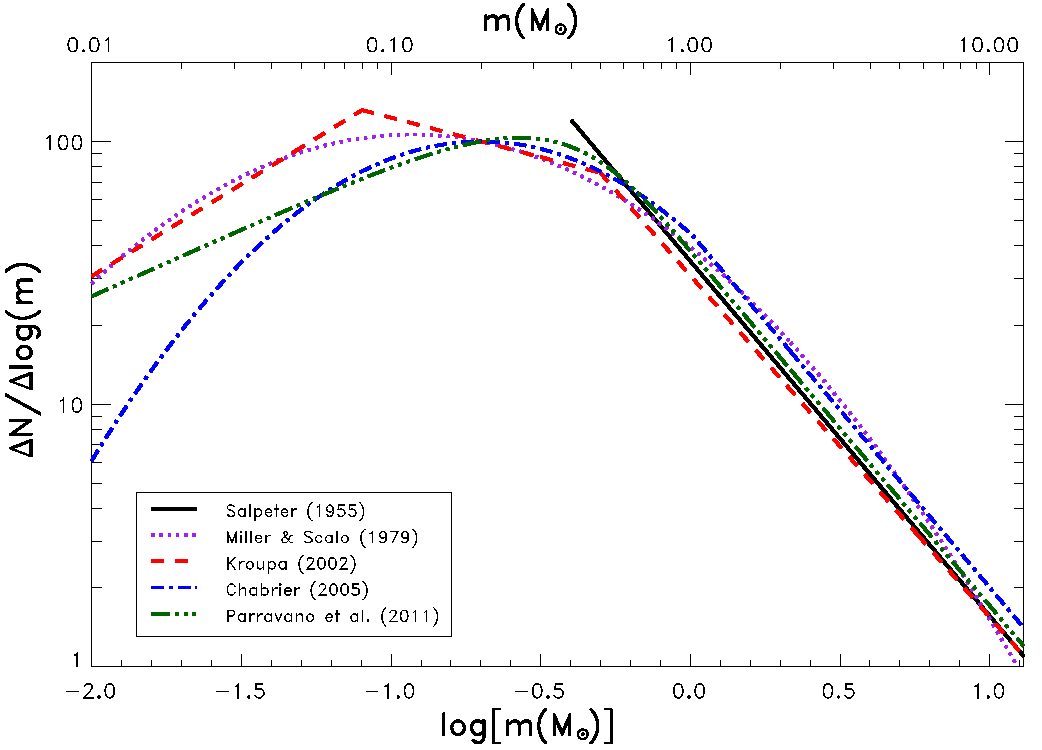
\includegraphics[width=1.0\textwidth]{imf_parameterization.pdf}
	\caption[IMF functional forms by various authors]{Functional forms representing the IMF of several stellar populations by the studies indicated in the label. All functions are normalized at 0.2 $M_\odot$, except for the \citet{Salpeter1955} slope.}
	\label{fig:IMFs}
\end{figure}

\subsubsection{Universality of the IMF}
One of the most challenging problems in modern astrophysics is the so-called \textit{universality} of the IMF, which refers to a possible null dependence of the IMF with the environmental conditions and/or time. Despite the diverse IMF functional forms mentioned in last section, the IMF of a vast diversity of stellar populations (dense clusters, associations, open clusters, globular clusters and field population) is well-described by a single representation, as found by \citet{Bastian2010}, working with the compilation from \citet{DeMarchi2010}. Nevertheless, significant scatter arise for the substellar regime, which can be due to uncertainties and/or incompleteness in the surveys. Similar results are obtained by \citet{Offner2014}, who focused on theories of the origin of the IMF and mostly comparing with regions in extreme circumstances where evidence of variations were presented. However, there are some studies showing significant variations of the IMF in the massive range such \citet{Weisz2015}, for a large sample of clusters in M31, and \citet{Dib2017}, by comparing the massive population of various young Galactic clusters with synthetic clusters from diverse IMF parameters. In a more general context, the study by \citet{Weidner-Kroupa2005} shows that the distribution of stellar masses across several entire galaxies is steeper than the stellar IMF.

These results in an apparent disagreement call for additional studies, specifically in the low-mass regime, for more robust conclusions about the nature of the IMF. As an example of the importance of the last phrase, one of the stellar associations most dispersed from the single underlying IMF by \citet{Bastian2010} is the Taurus Star-forming region, which exhibits an excess of LMSs, which disappears in the recent study by \citet{Luhman2018}, working with data from \ac{Gaia DR2} \citep{GaiaCollaboration2018}.
%Also important is the estimation of the IMF across the whole mass range of a stellar population and taking into account several issues such a spatial and photometric completeness as well as sources of contamination present in a photometric sample.

%A largely insensitive IMF to initial conditions would impply that star formation is a self-regulating process more than that based on the Jeans-mass argument.
%where the interactions between each other protostar and with the molecular cloud play the dominant role in the formation of the cluster.

%Even, there are attempts to establish a universal IMF for the astronomical objects in all scales across 36 orders of magnitude in mass, which is mostly represented for the slope $\Gamma=-1$ \citep{Binggeli-Hascher2007}.

To observationally determine the IMF of a stellar population, it is necessary to obtain first the luminosity function (\ac{LF}) of a sample of stars in a defined volume. Then, the LF is converted to the present day mass function (\ac{PDMF}) by assuming a mass-magnitude relationship. Finally, the PDMF is corrected by the star formation history, stellar evolution, cluster dynamical evolution, galactic structure and binarity to obtain the IMF. Each of these steps present difficulties on their own, which makes the IMF determination a non straightforward task \citep[e.g. ][]{Zinnecker2005,MaizApellaniz-Ubeda2005,Ascenso2011,Stassun2014b}. 

Various of the aforementioned difficulties in IMF studies are minimized when working with stellar clusters, in which, if young enough, the PDMF approximates to the IMF. However, an important issue to be taken into account in the analysis of stellar clusters is their dynamical evolution, which can produce a significant loss of members.

\subsection{Evolution of Young Clusters}
As mentioned at the beginning of this section, only a small fraction of young stellar systems keep as gravitational bound clusters after few tens of Myr. In fact, \citet{Lada-Lada2003} and \citet{Bonatto-Bica2011} found that only $\sim10\%$ of the young stellar systems remains as bound clusters for ages larger than 10 Myr. The evolution of these young systems depends on the variations of the gravitational potential when the parental cloud is expelled \citep[e.g. ][]{Baumgardt-Kroupa2007} and on their dynamical state \citep[contracting, expanding or in equilibrium, e.g.  ][]{Kuhn2018} as well as tidal perturbations by nearby and dense giant molecular clouds \citep{Kruijssen2012}.

The molecular gas present in embedded clusters is an important component than can be comparable in mass with the stellar content \citep[in the DR21 region; ][]{Schneider2010} or, even, can dominate the gravitational potential \citep[in the Orion Nebula Cluster, \ac{ONC}, except in the inner region; ][]{Stutz2018}. Gas expulsion due to stellar feedback (outflows, stellar winds, supernovae and photoionizing radiation) produces a decrease of the gravitational potential of the stellar systems, which in turn result in an expansion of the groups due to the velocity dispersion of the stars \citep{Baumgardt-Kroupa2007}. This process can result in an expanding unbound association if the gas remotion is fast \citep{Goodwin-Bastian2006}, explaining the deficit of observed clusters with ages larger than few tens of Myr \citep{Lada-Lada2003}. However, in more recent simulations, it is found that the gas expulsion effect is less important during the cluster disruption \citep{Parker-Dale2013,Dale2015}. Recently, \citet{Sills2018} found that the evolution of embedded clusters is more influenced by gravitational interactions between stars, with a small contribution from the surrounding gas.

However, recent studies in OB associations by \citet{Wright-Mamajek2018} and \citet{Ward-Kruijssen2018} show no clear evidence of expansion that can indicate that these associations had a more compact configuration in the past, which suggests they were not formed by the disruption of young stellar systems. These results support the idea that the star formation process is a structured process where the different components are formed \textit{in situ} i.e. a hierarchically process, more than in a monolithic scenario \citep[see the review by ][]{Gouliermis2018}.

However, additional evidence of expansion was presented by \citet{Getman2018} in young stellar populations in several star-forming regions and by \citet{Kuhn2018} in various young stellar clusters and associations. Also, \citet{Kounkel2018} found that the large stellar group structures that emerged from the molecular gas in the Orion Complex are preferentially expanding, but specific analysis are encouraged to determine the gravitational state (bound or not) of individual stellar systems in the complex.

Gravitational bound clusters are stellar systems with a total energy (kinematic energy plus gravitational energy) that is negative. A study to know if a stellar system is gravitationally bound can be done by comparisons of its velocity dispersion with the velocity dispersion necessary for a virial equilibrium \citep[e.g. ][]{Kuhn2018}. The important quantities for this analysis are 1D velocity dispersion which can be obtained from the radial velocity (\ac{RV}) and the total mass and its distribution that can be obtained from the determination of the IMF.

%As mentioned by \citep{Kuhn}, the... thus why we propose this project in a region that... with phot and spec analysis.
%	The processes of cluster assembly, equilibration, and disso- lution have remained poorly constrained by observation for two reasons: the difficulty of obtaining reliable sam- ples of cluster members in nebulous regions with many field star contaminants and the absence of kinematic information for faint stars.

%In this dissertation we present a characterization of the substellar and stellar population of a group that just emerged from its embedded phase. We focus on the determination of its mass spectrum across the whole mass range, from planetary-mass objects to intermediate/high-mass stars, to contribute to the understanding of the nature of its entire shape. Similarly important is the 
In this dissertation we present a characterization of the substellar and stellar population of a group that just emerged from its embedded phase. We focus on the determination of its mass spectrum across the whole mass range, from planetary-mass objects to intermediate/high-mass stars, together with a follow-up spectroscopy using several world-wide facilities, which allow us to determine if the group is gravitationally bound or not.

\subsection{25 Orionis Stellar Group}
An excellent stellar group to carry out the proposed study is 25 Orionis (\ac{25 Ori}), the most prominent overdensity in Orion OB1a \citep{Briceno2005,Downes2014,Briceno2018}. The physical properties that 25 Ori present allow a detailed analysis of its entire population. Fist, it is relatively close and has a low extinction ($365\pm47$ pc and $0.29\pm0.26$ mag, Su\'arez et al. 2018, submitted), which makes it possible to observe members with estimated masses lower than the deuterium burning limit (0.013 $M_\odot$). Also, it is young enough \citep[6.1$\pm$2.4; ][]{Briceno2018} to have lost massive members due to stellar evolution and to appear spatially concentrated to survey its entire spatial distribution, but old enough to have dispersed its parental cloud and have formed all its members as well as to keep a small fraction of members harboring circumstellar disks \citep{Briceno2005,Hernandez2007a,Downes2014}. More details about 25 Ori are found in Sections \ref{sec_IMF:introduction}, \ref{sec_IMF:mass-luminosity} and \ref{sec_BOSS:intro}.

%This dissertation is organized as follows: in Section \ref{sec:photometry} we carry out...
%which just emerged of its embedded phase, making it an interesting target to study the early evolution of a stellar system.
%An excellent stellar group to carry out a detailed study of the IMF across the whole mass range is 25 Orionis (\ac{25 Ori}), which just emerged of its embedded phase, making it an interesting target to study the early evolution of a stellar system.

%In this dissertation we presented a detailed study of the 

%%%%%%%%%%%%%%%%%%%%%%%%%%%%%%%%%%%%%%%%%
\newpage
\section[Photometric Analysis]{Photometric Analysis\ (Su\'arez et al. 2018, submitted)}
\label{sec:photometry}
The analysis presented in this section constitutes the publication ``System IMF of the 25 Ori Group from Planetary-mass Objects to Intermediate/High-mass Stars'' by Su\'arez et al. (2018, submitted to MNRAS in November, 2018), which was carried our as part of this dissertation.

%\subsection{Research Statement}
%\label{sec:rs_photometry}

{\bf Abstract.}
The stellar initial mass function (IMF) is an essential input for many astrophysical studies, but only in a few cases it has been determined for the whole mass spectrum, limiting the conclusions about the nature of its complete shape. The 25 Orionis group (25 Ori) is an excellent laboratory to investigate the IMF across the entire mass range, from planetary-mass objects to intermediate/high-mass stars. We combine new deep optical photometry with optical and near-infrared data from the literature to select 1687 member candidates covering a 1.1$^\circ$ radius area in 25 Ori. With this sample we derived the 25 Ori system IMF from 12 $M_{Jup}$ to 13 $M_\odot$. This system IMF is well described by a three-part power-law with $\Gamma=-0.78\pm0.06$, $0.91\pm0.11$ and $1.48\pm0.18$ for $m\le0.3\ M_\odot$, $0.3< m/M_\odot<1.0$, and $m\ge1.0\ M_\odot$, respectively. It is also described by a lognormal function with $m_c=0.31\pm0.04$ and $\sigma=0.46\pm0.05$ for $m<1\ M_\odot$. The best tapered power-law representation of the entire system IMF has $\Gamma=1.10\pm0.09$, $m_p=0.31\pm0.03$ and $\beta=2.11\pm0.09$. This system IMF does not present significant variations with the radii. We compared the resultant system IMF as well as the substellar/stellar ratio of $0.15\pm0.03$ we estimated for 25 Ori with that of other stellar regions with diverse conditions and found no significant discrepancies. These results support the idea that general star formation mechanisms are probably not strongly dependent to environmental conditions. We found that the substellar and stellar objects in 25 Ori have similar spatial distributions and confirmed that 25 Ori is a gravitationally unbound stellar group.

\subsection{Introduction}
\label{sec_IMF:introduction}

The mass spectrum of the members of a stellar population at birth is known as initial mass function (IMF). The IMF is the main product of the star formation process and is one of the fundamental astrophysical quantities. Since the seminal IMF study by \citet{Salpeter1955}, there have been many contributions to this topic to understand the origin and behavior of the IMF, but only few of them focus on the whole mass range of the populations, which limits the conclusions about its complete shape \cite[e.g.][and references therein]{Bastian2010}.

Observational IMF studies in a complete range of masses, from planetary-mass objects to massive star scales, allow to analyze the continuity of the star formation process over about three orders of magnitude of mass and help to constrain initial conditions of star formation models. These kind of studies are also important to understand if the star formation process is sensitive or not to environmental conditions and if it change in time, which is the nature of the so-called \textit{universality of the IMF} \cite[e.g.][]{Kroupa2013,Offner2014}.

Young stellar clusters ($\lesssim 10$ Myr) are useful laboratories for observational studies of the IMF in a wide range of masses because objects are brighter in the pre-main sequence (\ac{PMS}) phase than on the main sequence (\ac{MS}), none or minimum correction by the stellar evolution of their members is necessary, their spatial distributions are relatively small (for groups beyond the solar neighborhood) and their members have basically the same age, metallicity (\ac{Z}) and distance. However, an important issue to be taken into account when working with embedded clusters \citep[$\lesssim3$ Myr; ][]{Lada-Lada2003} is dust extinction, which, on one hand, complicates the detection of the least massive objects but, on the other hand, helps to separate the cluster population from the background contamination. Another important issue when studying stellar clusters is their dynamical evolution over time, causing a loss of the low-mass members, becoming dynamically mass segregated \citep[e.g., ][]{Elmegreen2000}. About 10\% of the low-mass stars (LMSs) and brown dwarfs (BDs) are expected to be lost for clusters with ages of about 100 Myr \citep{deLaFuenteMarcos-deLaFuenteMarcos2000}. Therefore, for stellar clusters with an age between 5 and 10 Myr there is a good compromise between extinction, youth and dynamical evolution for a complete determination of the IMF.

The best studied clusters in the literature in terms of their IMFs over a wide mass range are: Pleiades \citep[0.03~-~10 $M_\odot$;][]{Moraux2003}, Blanco 1 \citep[0.03~-~3 $M_\odot$;][]{Moraux2007a}, Collinder 69 \citep[0.016~-~20 $M_\odot$;][]{Bayo2011}, $\sigma$ Ori \citep[0.006~-~19 $M_\odot$;][]{PenaRamirez2012}, the Orion Nebula Cluster \citep[ONC; 0.025~-~3 $M_\odot$, $\approx$0.005~-~1 $M_\odot$;][respectively]{DaRio2012,Drass2016}, and RCW 38 \citep[0.02~-~20 $M_\odot$;][]{Muzic2017}. In all these studies the IMF was not corrected by unresolved multiple systems, therefore, it refers to the so-called {\it system} IMF instead of the single-star IMF \citep{Chabrier2003a}. However, \citet{Moraux2003} and \citet{Muzic2017} also present the single-star IMF. In Table \ref{tab_IMF:imf_literature} we summarize the resulting parameterizations of these system IMFs as well as the employed theoretical models for mass determination. For parameterizations of a larger sample of clusters but in smaller mass ranges see Table 1 from \citet{DeMarchi2010} and Table 4 from \citet{Muzic2017}, mainly, for low-mass stars. Although the tables indicated above show some differences between the various IMFs, more complete and systematic observational studies are needed in populations with different environments and evolutionary stages before any claim concerning variations of the IMF, as suggested by \citet{Bastian2010} and \citet{Offner2014}.

\begin{table*} \tiny
 \caption{System IMF parameterizations over a wide mass range in several young clusters.}
 \label{tab_IMF:imf_literature}
 \begin{threeparttable}
  \begin{tabular}{@{\extracolsep{2pt}}lcccccccccc@{}}
   \toprule
 	Cluster      & Age   &       \multicolumn{3}{c}{Lognormal}          &         \multicolumn{4}{c}{Power Law}                & Model  & Ref  \\
   \cline{3-5}
   \cline{6-9}
 	             &       & $m_c$         &    $\sigma$   & $m$ range    & $\Gamma_1^a$ & $m$ range   & $\Gamma_2^b$  & $m$ range   &        & \\
 	             & [Myr] & [$M_\odot$]   &               & [$M_\odot$]  &              & [$M_\odot$] &               & [$M_\odot$] &        & \\
%    Unit & Unit & Unit & Unit & Unit & Unit & Unit & Unit & Unit & Unit \\
   \midrule
   \multirow{2}{*} {RCW 38} & \multirow{2}{*} {1$^c$} &               &               &              & -0.29$\pm$0.11     & 0.02-0.50  & 0.60$\pm$0.13     & 0.50-20 & \multirow{2}{*} {BT-Settl+PARSEC} & \multirow{2}{*} {1} \\
                            &       &               &               &              & -0.58$\pm$0.18     & 0.02-0.20  & 0.48$\pm$0.08     & 0.20-20 &                                   &                     \\
   \multirow{2}{*} {ONC} & \multirow{2}{*} {2} & 0.35$\pm$0.02$^d$ & 0.44$\pm$0.05$^d$ & \multirow{2}{*} {0.025-3} & -1.12$\pm$0.90$^d$     & 0.025-0.30 & 0.60$\pm$0.33$^d$     & 0.30-3  & NextGen & \multirow{2}{*} {2} \\
                         &   & 0.28$\pm$0.02 & 0.38$\pm$0.01     &                           & -2.41$\pm$0.25     & 0.025-0.17 & 1.30$\pm$0.09     & 0.17-3  & DM98 &                                    \\
   \multirow{2}{*} {$\sigma$ Ori} & \multirow{2}{*} {3$^e$} & 0.24$\pm$0.09$^f$ & 0.53$\pm$0.19$^f$ & 0.006-1  & \multirow{2}{*} {-0.40$\pm$0.20} & \multirow{2}{*} {0.006-0.35} & \multirow{2}{*} {0.70$\pm$0.20} & \multirow{2}{*} {0.35-19} & \multirow{2}{*} {Siess+Lyon} & \multirow{2}{*} {3} \\
                                  &       & 0.27$\pm$0.09$^f$ & 0.63$\pm$0.15$^f$ & 0.006-19 &                                  &                              &                                 &                           &                                  &                                           \\
   Collinder 69 & 4-6$^g$     &              &               &              & -0.71$\pm$0.10$^h$ & 0.01-0.65  & 0.82$\pm$0.05$^h$ & 0.65-25 & Siess+COND    & 4 \\
   Blanco 1     & 100-150     &0.36$\pm$0.07 & 0.58$\pm$0.06 & 0.03-3       & -0.31$\pm$0.15     & 0.03-0.60  &                   &         & NextGen+DUSTY & 5 \\
   Pleiades     & 125$^i$     & 0.25          & 0.52          & 0.03-10      & -0.40$\pm$0.11     & 0.03-0.48  & 1.7               & 1.5-10  & NextGen       & 6 \\
   \bottomrule
  \end{tabular}
  \begin{tablenotes}[para,flushleft]
    $^a$For LMSs and BDs.\\
    $^b$For intermediate/high-mass stars.\\
    $^c$\citet{Getman2014b}.\\
    $^d$For sources older than 1 Myr.\\
    $^e$\citet{ZapateroOsorio2002}.\\
    $^f$Mean values of the two set of parameters obtained combining \citet{Baraffe1998} and \citet{Siess2000} models at different cutoffs (0.3 and 1 $M_\odot$).\\
    $^g$\citet{Dolan1999}.\\
    $^h$Mean value of the six reported values and the error as the standard deviation.\\
    $^i$\citet{Stauffer1998}.\\

    NextGen: \citet{Baraffe1998}, DM98: \citet{DAntona1998}, Siess: \citet{Siess2000}, DUSTY: \citep{Chabrier2000}, COND: \citep{Baraffe2003}, Lyon: NextGen, DUSTY and COND, \ac{BT-Settl}: \citet{Baraffe2015}, and \ac{PARSEC}: \citet{Bressan2012} and \citet{Chen2014}.\\

    References: (1) \citet{Muzic2017}, (2) \citet{DaRio2012}, (3) \citet{PenaRamirez2012}, (4) \citet{Bayo2011}, (5) \citet{Moraux2007a}, and (6) \citet{Moraux2003}.
  \end{tablenotes}
 \end{threeparttable}
\end{table*}

An interesting young stellar group for studying the IMF over its whole mass range and full spatial extent is 25 Orionis (25 Ori), the most prominent spatial overdensity of PMS stars in Orion OB1a, originally detected by \citet{Briceno2005}. The estimated radii for this group are 1.0$^\circ$, 0.5$^\circ$ and 0.7$^\circ$ by \citet{Briceno2005,Briceno2007}, \citet{Downes2014} and \citet{Briceno2018}, respectively. This makes it feasible to perform an observational study covering the full spatial extent of this group. 25 Ori is a 7-10 Myr population located at 356$\pm$47 pc and presents a low visual extinction (\ac{Av}) of 0.29$\pm$0.26 mag (see Appendices \ref{sec_app_IMF:distance} and \ref{sec_app_IMF:extinction}), which facilitates the detection of members down to planetary-masses \citep{Downes2015}. Several previous studies have focused on characterizing the 25 Ori population; \citet{Kharchenko2005,Kharchenko2013} for intermediate/high-mass stars, \citet{Briceno2005,McGehee2006,Briceno2007,Hernandez2007a,Biazzo2011,Downes2014,Suarez2017,Briceno2018} for LMSs and \citet{Downes2015} for the very low-mass and BD members.

In 2014, \citeauthor{Downes2014} reported the first and only available determination of  the system IMF of 25 Ori in the mass range $0.02\lesssim m/M_\odot\lesssim 0.8$ working with a sample of photometric member candidates inside an area of 3x3 deg$^2$ around 25 Ori. In this work we improve the 25 Ori system IMF by including optical and near-infrared (\ac{NIR}) photometry spanning from intermediate/high-mass stars down to planetary-mass objects ($0.012\le m/M_\odot\le13.1$) and also covering its full spatial extent. In Section \ref{sec_IMF:data}, we present our observations and public catalogs used in this study. The selection of the photometric member candidates and a discussion of different issues that could affect the determination of the IMF, in the particular case of 25 Ori, and how we deal with them are presented in Section \ref{sec_IMF:candidates}. In Section \ref{sec_IMF:results}, we present the derivation of the 25 Ori system IMF and the comparisons with other associations, and the analysis of the spatial distribution, the BD frequency and the gravitational state of 25 Ori. Finally, a summary and conclusions are given in Section \ref{sec_IMF:conclusions}.

\subsection{Photometric Data}
\label{sec_IMF:data}

\subsubsection{DECam observations}
\label{sec_IMF:DECam}

This work includes new very deep optical \textit{i}-band photometry of 25 Ori obtained using the Dark Energy Camera (\ac{DECam}) mounted on the 4m Victor M. Blanco telescope at CTIO. DECam is a 570 Megapixel camera with an array of 62 2kx4k detectors with a plate scale of $0.263''$ pixel$^{-1}$, covering a field of view (\ac{FOV}) of 1.1$^\circ$ radius \citep{Flaugher2015}. Our DECam observations were performed on Feb 24, 2016 (PI: G. Su\'arez). We obtained 11x300s exposures in the $i$-band centered at $\alpha_{J2000}= 05^{\rm h} 25^{\rm m} 04^{\rm s}.8$ and $\delta_{J2000} = +01^{\circ} 37' 48''.6$ with an airmass $<1.3$ and a mean seeing of $\sim 0.9''$. During our observations two DECam detectors were not functional, reducing the array to 60 usable detectors. In Section \ref{sec_IMF:spatial} we discuss how this fact, together with the gaps and the non circular configuration of the detectors, affect the spatial coverage of the DECam observations. In Figure \ref{fig_IMF:sky} we show the spatial coverage of our DECam data.

The reduced and calibrated data were produced by the DECam Community Pipeline \citep{Valdes2014} and downloaded from the NOAO Science Archive\footnote{\url{http://archive.noao.edu/}}. The resulting data have processing level of 2, which means they are single reduced frames after removing the instrument signature and applying the WCS and photometric calibrations, as explained in the NOAO Data Handbook\footnote{\url{http://ast.noao.edu/sites/default/files/NOAO\_DHB\_v2.2.pdf}}.

We combined the individual frames using the \texttt{imcombine} routine of IRAF\footnote{IRAF is distributed by NOAO, which is operated by AURA, Inc., under cooperative agreement with the NSF.}, considering a ccdclip value of 3.5$\sigma$ and correcting the offset of the individual images using the WCS solutions provided by the NOAO pipeline. The photometry was made using a modification of the $PinkPack$ pipeline \citep{Levine2006} to work with the DECam data, which uses the SExtractor software \citep{Bertin-Arnouts1996} for the detections, IRAF/APPHOT for the aperture photometry and IRAF/DAOPHOT for the PSF photometry. To calibrate the resulting $i$-band photometry we added the zero point of 25.18 mag for our DECam observations and an offset of 0.637 mag with respect to the $i$-band photometry in the DECam system obtained from the Sloan Digital Sky Survey (\ac{SDSS}) Data Release 9 (DR9) \citep{Ahn2012} catalog. More details about this calibration are found in Appendix \ref{sec_app_IMF:DECam_calibration}. The mean value of the residuals between our calibrated data and those in the DECam system using photometry from SDSS is -0.001 mag with a root mean square (\ac{RMS}) of 0.038 mag.

\begin{figure*}[ht!]
	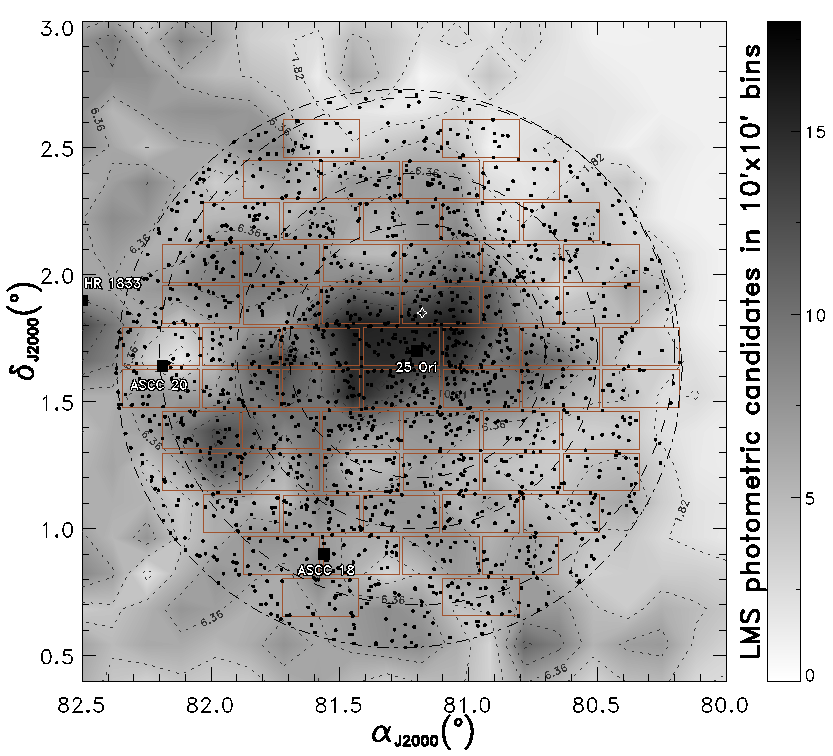
\includegraphics[width=1.0\textwidth]{f_1.pdf}
	\caption[Spatial distribution of our photometric member candidates.]{Spatial distribution of our photometric member candidates (black points; see Section \ref{sec_IMF:candidates}). The dash-dotted circle shows the FOV of our DECam observations obtained with the array of detectors indicated by the brown boxes. The dashed circles indicate, from the center outwards, the 25 Ori estimated areas by \citet[0.5$^\circ$ radius; ][]{Downes2014}, \citet[0.7$^\circ$ radius; ][]{Briceno2018} and \citet[1.0$^\circ$ radius; ][]{Briceno2005,Briceno2007} centered at $\alpha_{J2000}=81.2^\circ$ and $\delta_{J2000}=1.7^\circ$. The black squares indicate the labeled stellar groups (25 Ori by \citealt{Briceno2005}, ASCC 18 and ASCC 20 by \citealt{Kharchenko2013} and HR 1833 by \citealt{Briceno2018}). The gray background map indicates the density of LMS and BD photometric member candidates of Orion OB1a in 10'x10' bins \citep{Downes2014}. The white star symbol shows the position of the 25 Ori star.}
	\label{fig_IMF:sky}
\end{figure*}

\subsubsection{CIDA Deep Survey of Orion}
\label{sec_IMF:CDSO}
Additional optical $I_c$-band photometry for sources brighter that the DECam saturation limit (see Section \ref{sec_IMF:sensitivity}) was obtained from the CIDA Deep Survey of Orion \citep[\ac{CDSO}; ][]{Downes2014}. This catalog was constructed by coading the photometry from the CIDA Variability Survey of Orion \citep[\ac{CVSO}; ][]{Briceno2005,Mateu2012,Briceno2018}, obtained at the National Astronomical Observatory of Venezuela. The area covered by this survey extends beyond the limits of our DECam data.

\subsubsection{VISTA Orion Survey}
\label{sec_IMF:VISTA}
The deep $Z$, $J$ and $K$ near-infrared photometry for this study is from the \ac{VISTA} (Visible and Infrared Survey Telescope for Astronomy) survey in Orion \citep{Petr-Gotzens2011}, which was carried out as part of the VISTA science verification program \citep{Arnaboldi2010} with the near-infrared camera (VIRCAM) mounted on the 4.2m telescope at Paranal Observatory.

\subsubsection{Photometry from Literature}
\label{sec:catalogs}
\subsubsubsection{Optical Photometry}
The optical data from DECam and the CDSO were complemented with the $i$-band photometry from the fourth \ac{USNO} (United States Naval Observatory) CCD Astrograph Catalog \ac{UCAC4} \citep{Zacharias2013} as well as the $I_c$-band photometry from the $Hipparcos$ catalog \citep{Perryman1997} for the brightest sources in 25 Ori.

\subsubsubsection{Near-IR Photometry}
We complemented the VISTA near-infrared photometry with $J$ and $Ks$-band photometry from the Two Micron All Sky Survey (\ac{2MASS}) catalog \citep{Skrutskie2006}.

In Table \ref{tab_IMF:catalogs} we summarized the spatial coverage of 25 Ori (for an area of 0.7$^\circ$ radius, see Section \ref{sec_IMF:spatial}), the spatial resolution and the photometric sensitivities (see Section \ref{sec_IMF:sensitivity}) of the optical and NIR catalogs used in this study. The masses corresponding to the saturation and completeness magnitudes are obtained using the mass-luminosity relation explained in Section \ref{sec_IMF:mass-luminosity}.

\begin{table*}
\caption[Information of the photometric catalogs.]{Spatial coverage of 25 Ori$^1$ and photometric sensitivities of the catalogs used in this study.}
%\begin{center}
  \small
  \label{tab_IMF:catalogs}
  \begin{threeparttable}
 	%\begin{tabular}{@{}p{1.1cm}p{0.5cm}p{0.8cm}cccccp{0.1cm}}
    \setlength{\tabcolsep}{12pt}
 	\begin{tabular}{lcccccccc}
    \toprule
 	Survey      & Phot.    & FWHM      & Area         & Satur.       & Comp.        & Satur.     & Comp.       &  Ref. \\%& Limiting  \\
 	            & Band     & (arcsec)  & [per cent]         & (mag)        & (mag)        & ($M_\odot$)& ($M_\odot$) &       \\%& (mag)     \\
    \midrule
 	DECam       & $I_c$    & 0.9       & $\approx 86$ & 16.0         & 22.50        & 0.16       & 0.012       & a     \\%& 25.0      \\
 	CDSO        & $I_c$    & 2.9       & 100          & 13.0         & 19.75        & 0.86       & 0.020       & b     \\%& 21.5      \\ 
 	UCAC4       & $I_c$	   & 1.9       & 100          & 7.0          & 14.75        & 6.33       & 0.340       & c     \\%& 16.0      \\
 	$Hipparcos$ & $I_c$	   & ---       & 100          & $<$5.0       & ---          & $>$13.5    & ---         & d     \\%& 16.0      \\
 	VISTA       & $J$      & 0.9       & 100          & 12.0         & 20.25        & 0.85       & $<$0.010    & e     \\%& 21.5      \\
 	2MASS       & $J$      & 2.5       & 100          & 4.0          & 16.25        & 19.3       & 0.287       & f     \\%& 17.0      \\
    \bottomrule
 	\end{tabular}
  \begin{tablenotes}[para,flushleft]
    $^a$Considering an area of $0.7^\circ$ radius.\\
	References: (a) This work; (b) \citet{Downes2014}; (c) \citet{Zacharias2013}; (d) \citet{Perryman1997}; (e) \citet{Petr-Gotzens2011}; (d) \citet{Skrutskie2006}
  \end{tablenotes}
 \end{threeparttable}
\end{table*}

\subsubsection{Merged Optical-NIR Catalog}
\label{sec_IMF:merged_cat}

From the individual catalogs with optical and NIR data we constructed one single general catalog, as explained in this section.

\subsubsubsection{Transformation of optical photometry into Cousins system}
\label{sec_IMF:photometry_transformation}
We transformed the $i$-band photometry from UCAC4 and DECam to the Cousin system $I_c$-band, which is a photometric band predicted by the BT-Settl \citep{Baraffe2015} and \ac{PARSEC-COLIBRI} \citep{Marigo2017} isochrones used to estimate masses to later construct the system IMF in Section \ref{sec_IMF:mass-luminosity}. To obtain the $I_c$ magnitudes from UCAC4 we used the empirical transformations by \citet{Jordi2006}, which relate SDSS photometry with other photometric systems included the Cousins system. For the DECam photometry we derived directly from our data color-dependent transformations to convert the calibrated DECam magnitudes to the SDSS system and then to the Cousins system. The RMS we obtained when comparing the $I_c$ magnitudes from the CDSO and those from UCAC4 and from DECam after the transformation are 0.07 and 0.04 mag, respectively. The details about these transformations are described in Appendix \ref{sec_app_IMF:photometry_transformation}. Because the Cousins photometric system is already used by the CDSO and $Hipparcos$ catalogs, after the transformation of the DECam and UCAC4 photometries, the complete sample of optical observations are all in the same photometric system.

\subsubsubsection{Photometric uncertainties}
\label{sec_IMF:photometry_uncertainties}
Before we define the brightness ranges where each catalog will be used, we fitted exponential functions to the photometric uncertainties of the optical and NIR catalogs with respect to the magnitude ($\delta I_c(I_c)$ for the optical data and $\delta J(J)$ for the NIR data). This way we can estimate the uncertainties of the data as a function of the photometric magnitudes, which will allow us to combine the catalogs considering the typical photometric uncertainties at each brightness point where the catalogs are joined. In Table \ref{tab_IMF:errors} we show the parameters for each catalog, working with magnitudes inside their saturation and completeness limits (see Section \ref{sec_IMF:sensitivity}).

\begin{table}
\caption[Parameters of the exponentials fitted to the photometric errors of the optical and NIR catalogs.]{Parameters of the exponentials fitted to the photometric uncertainties of the optical and NIR catalogs used in this study.}
  \small
  \label{tab_IMF:errors}
  \setlength{\tabcolsep}{18pt}
  \begin{center}
  \begin{threeparttable}
 	\begin{tabular}{lcccc}
 	%\begin{tabular}{p{0.8cm}p{0.3cm}p{0.5cm}p{0.4cm}p{0.4cm}p{0.4cm}p{0.4cm}p{0.1cm}}
    \toprule
 	Catalog & Photometric &  $a$  &  $b$   & $c$   \\
			& Band        &       &        &       \\
    \midrule
 	DECam   & $I_c$	& 0.005 & 25.861 & 1.042 \\
 	CDSO    & $I_c$	& 0.002 & 22.175 & 0.999 \\
 	UCAC4   & $I_c$	& 0.037 & 8.993  & 0.453 \\
 	VISTA   & $J$	& 0.002 & 16.870 & 0.732 \\
 	2MASS   & $J$	& 0.024 & 20.240 & 1.105 \\
    \bottomrule
 	\end{tabular}
  \begin{tablenotes}[para,flushleft]
	Note. The exponentials have the form $f(x)=a+e^{(cx-b)}$, where $x$ is the magnitude in the corresponding photometric band.
  \end{tablenotes}
 \end{threeparttable}
 \end{center}
\end{table}

\subsubsubsection{Cutoffs and merged catalogs}
\label{sec_IMF:cutoffs}
The brightness ranges where each photometric catalog was used are related to their photometric sensitivities, which are described in Section \ref{sec_IMF:sensitivity} and reported in Table \ref{tab_IMF:catalogs}. The $I_c$-band photometry we used to have a combined optical catalog are as follows: $i)$ UCAC4 for $I_c<13.0+\delta I_c(13.0)$, $ii)$ CDSO for $13.0-\delta I_c(13.0)\leq I_c<17.0+\delta I_c(17.0)$, and $iii)$ DECam for $I_c\geq 17.0-\delta I_c(17.0)$. We also added 25 stars (including 25 Ori) from the $Hipparcos$ catalog, which are too bright to have $I_c$ magnitudes from UCAC4. The $J$-band photometry used to have a combined NIR catalog are as follows: $i)$ 2MASS for $J<13.0+\delta J(13.0)$, and $ii)$ VISTA for $J\geq 13.0-\delta J(13.0)$. Then, we removed 3$^{\prime\prime}$ duplicates from the optical and NIR catalogs and kept the sources with smaller photometric uncertainties. To join the optical and NIR catalogs we did a cross-match between them with a tolerance of 3$^{\prime\prime}$ using STILTS\footnote{\url{http://www.star.bris.ac.uk/~mbt/stilts/}} \citep{Taylor2006}.

The final optical and NIR catalog has 110527 detections inside an area of 1.1$^\circ$ radius in 25 Ori, being most of them (about 85\%) from the DECam and VISTA catalogs.

\subsection{Selection of Photometric Candidates}
\label{sec_IMF:candidates}

\subsubsection{PMS Locus}
\label{sec_IMF:locus}
The use of color-magnitude diagrams (\ac{CMD}s) combining optical and NIR data has been successfully tested for identifying young stellar objects \citep[e.g. ][ and references therein]{Downes2014}. We selected photometric member candidates from the merged optical and NIR catalog according to their position in the $I_c$ vs $I_c-J$ diagram shown in Figure \ref{fig_IMF:CMD}.

To define the PMS locus in which the member candidates lie, we plotted a large set of 355 spectroscopically confirmed low-mass members of 25 Ori from \cite{Briceno2005,Briceno2007,Downes2014,Suarez2017,Briceno2018} and 15 spectroscopically confirmed very low mass and BD members of 25 Ori and Orion OB1a from \citet{Downes2015}. Most of these members were confirmed through similar spectroscopic procedures, which makes the sample more homogeneous. Additionally to the confirmed members, we also plotted 38 highly probable intermediate/high-mass members from \cite{Kharchenko2005}. The final sample of 408 spectroscopically confirmed members and highly probable members covers the spectral type range from B2 to M9 and trace a clear sequence in the $I_c$ vs $I_c-J$ diagram. This sequence corresponds to the empirical isochrone of 25 Ori, which was defined averaging the $I_c-J$ colors per $I_c$-bin (red dashed curve in Figure \ref{fig_IMF:CMD}). The resulting empirical isochrone is roughly consistent with the PARSEC-COLIBRI and BT-Settl 7 Myr isochrones. This empirical isochrone was our starting point to define the PMS locus considering the following uncertainties and effects:

$i)$ \emph{Distance uncertainty.} From the sample of spectroscopically confirmed members of 25 Ori, we obtained a mean distance of 356 pc with a standard deviation, $\sigma$, of 47 pc, considering the distances reported by \citet[\ac{BJ18}; ][]{Bailer-Jones2018} on the basis of Gaia parallaxes \citep[Gaia DR2; ][]{GaiaCollaboration2018}. We considered only distances with uncertainties smaller than 20\% (more details in Appendix \ref{sec_app_IMF:distance}). Then, we broaden vertically the edges of the PMS locus in the CMD by adding the 1-$\sigma$ uncertainty in distance, which corresponds to upwards and downwards offsets of 0.31 and 0.27 mag, respectively.

$ii)$ \emph{Age uncertainty.} To estimate the change in the $I_c$ brightness ($\Delta I_c$) as a function of the $I_c-J$ color due to the uncertainty of the 25 Ori age \citep[6.1$\pm$2.4; ][]{Briceno2018}, we worked with the PARSEC-COLIBRI and BT-Settl isochrones. We obtained $\Delta I_c^I$ between the isochrone corresponding to the age of 25 Ori and that for the 25 Ori age minus the error. Similarly, we obtained $\Delta I_c^{II}$ considering the age of 25 Ori and the age plus the error. In most of the color range considered (-0.5-4.5 mag), $\Delta I_c^I$ is larger than $\Delta I_c^{II}$. We used $\Delta I_c^I$ to move upwards the upper edge of the locus and $\Delta I_c^{II}$ to move downwards the lower edge.

$iii)$ \emph{Unresolved binarity.} According to \citet{Briceno2007}, the observed spread in the CMD of young stars in the 25 Ori field is roughly consistent with the upper limit of 0.75 mag expected from unresolved binaries. Thus, we used this limit to move upward the upper edge of the locus.

$iv)$ \emph{Mean intrinsic variability.} We characterized the $I_c$-amplitude variations as a function of the magnitude for the 25 Ori member candidates from \citet{Downes2014} using the CVSO catalog. These variations range between 0.2 and 0.9 mag for candidates with $I_c$ magnitudes between 13.0 to 19.0. For brighter and fainter $I_c$ magnitudes we assumed these minimum and maximum variation limits, respectively. Thus, we used these $I_c$-amplitude variations to move upwards and downwards the upper and lower edges of the locus, respectively. For the $J$-band, \citet{Scholz2009} reported the low-level amplitude variations of about 0.2 mag for young LMSs and BDs. Assuming that when occurs a maximum or a minimum in the $I_c$-brightness of a variable source also takes place the maximum or minimum in the $J$-band brightness, we considered $I_c-J$ amplitude variations as the difference between the $I_c$-amplitude variations and the representative 0.2 mag variations in the $J$-band to move leftwards and rightwards the blue (lower) and red (upper) edges of the locus, respectively.

$v)$ \emph{Photometric uncertainties.} We considered the exponentials fitted to the uncertainties of the optical and NIR catalogs as a function of the magnitudes to move both edges of the locus. The upper and lower edges were moved upwards and downwards, respectively, according to the uncertainty corresponding to each $I_c$-magnitude of the optical catalogs used in the different ranges. The blue (lower) and red (upper) edges of the locus were moved leftwards and rightwards, respectively, considering the uncertainties added in quadrature for each $I_c$ and $J$-magnitude from the catalogs used in the different ranges.

The sources lying inside this resulting PMS locus were selected as photometric member candidates of 25 Ori. We selected 1694 candidates inside the DECam FOV having $I_c$ magnitudes from 5.08 to 23.3.

The locus defined this way contains about 95\% of the confirmed members and highly probable members of 25 Ori. From the members lying out, on the left side, of the PMS locus, about 75\% of them have $>99$\% probability of being variable stars in the CVSO. In Section \ref{sec_IMF:missed} we estimated that the fraction of 25 Ori members we can lose in our photometric selection is $\sim3.1$\%.

It is important to notice in Figure \ref{fig_IMF:CMD} that in the $I_c$ range roughly between 9 and 13 mag, the giant and subgiant branches cross the PMS locus, which increases the contamination by these sources in this brightness range. We discussed in Section \ref{sec_IMF:fieldcontam} how to deal with this contamination.

\begin{figure*}[ht!]
	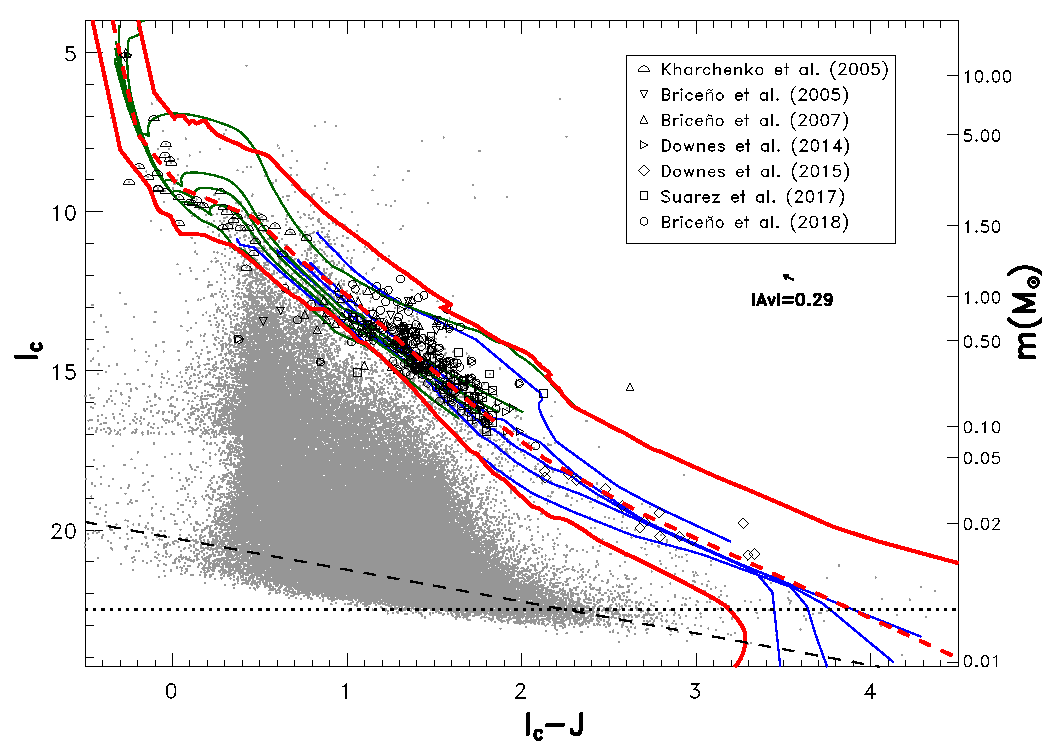
\includegraphics[width=1.0\textwidth]{f_2.pdf}
	\caption[$I_c$ vs $I_c-J$ diagram for the selection of the photometric member candidates.]{CMD used for the selection of photometric member candidates of 25 Ori. The red solid curves show the PMS locus defined considering the empirical isochrone (red dashed curve) and several issues that may affect the position of the sources in this plot. The open symbols represent the known spectroscopically confirmed members \citep{Briceno2005,Briceno2007,Downes2014,Downes2015,Suarez2017,Briceno2018} and high-probable members \citep{Kharchenko2005} of 25 Ori, as shown in the label, which trace the empirical isochrone. The gray dots indicate all the detections in our combined optical and NIR catalog. The black dotted and black dashed lines show the $I_c$/DECam and $J$/VISTA completeness magnitudes, respectively. The blue and green curves indicate, respectively, the BT-Settl and PARSEC-COLIBRI isochrones for ages, from top to bottom, of 1, 5, 7, 10 and 20 Myr. The arrow shows the dereddening vector for the mean extinction of 25 Ori. Masses from the mentioned models for an age of 7 Myr, distance of 356 pc and visual extinction of 0.29 mag are labeled in the right axis. The giants and subgiants branches cross the PMS locus close to (0.9, 13) and (0.5, 11), respectively.}
	\label{fig_IMF:CMD}
\end{figure*}

\subsubsection{Sources of Uncertainty, Contamination and Biases}
\label{sec_IMF:uncertainties}
Several previous works have studied the uncertainties and biases implicit in the observational determination of the IMF \citep[e.g.][]{Moraux2003,Moraux2007a,Moraux2007b,Ascenso2011,Dib2017}. In this section we characterize these effects in the case of 25 Ori and show how we corrected them.

\subsubsubsection{Spatial Completeness}
\label{sec_IMF:spatial}
The CDSO and VISTA catalogs and all the public catalogs considered in this work have a full spatial coverage of the FOV of the DECam observations.

As explained in Section \ref{sec_IMF:DECam}, our DECam observations were obtained with an array of 60 detectors configured as shown in Figure \ref{fig_IMF:sky} (brown boxes), therefore, part of the area in a FOV is lost by the gaps and because the array is not circular. To compute what fraction of a FOV is covered by the DECam data, we used the Monte Carlo method to generate a list of sources randomly distributed inside the FOV and counting those lying inside the detectors. We found this way that for the DECam FOV, the DECam data cover $\approx70$\% of the area. If we consider the previously estimated areas of 25 Ori, the DECam observations have a coverage of $\approx 79$\% when considering \citet[1.0$^\circ$ radius; ][]{Briceno2005,Briceno2007} and $\approx86$\% when considering \citet[0.7$^\circ$ radius; ][]{Briceno2018} or \citet[0.5$^\circ$ radius; ][]{Downes2014}. These fractions will allow us to correct the luminosity function (LF) and system IMF of 25 Ori by the spatial coverage of the DECam data. In Table \ref{tab_IMF:catalogs} we report the spatial coverage of 25 Ori for all the catalogs used in this study.

In Table \ref{tab_IMF:candidates} we list the number of member candidates inside the DECam FOV after applying the correction by the spatial coverage of the DECam data. If we had a full coverage of the DECam observations, we would expect 1782 photometric member candidates in the $I_c$ range from 5.08 to 23.3 mag. The mass range corresponding to this brightness range is obtained in Section \ref{sec_IMF:sys-imf}.

\subsubsubsection{Photometric Sensitivity}
\label{sec_IMF:sensitivity}
The saturation and completeness magnitudes for the optical and NIR catalogs were determined, respectively, as the brightest and faintest magnitudes between which the logarithmic number of sources per magnitude bin do not deviate from a linear behavior. We estimated the masses corresponding to these magnitudes using the BT-Settl and PARSEC-COLIBRI 7 Myr isochrones. In Table \ref{tab_IMF:catalogs} we summarize these values, where we can see how the optical and NIR catalogs complement each other. Therefore, in the determination of the LF and system IMF of 25 Ori, for the sources more massive than the DECam completeness mass (0.012 $M_{Jup}$), it is not necessary to make any correction due to the photometric sensitivity of the catalogs.

\subsubsubsection{Contamination by Field Stars}
\label{sec_IMF:fieldcontam}
Though the use of optical-NIR CMDs allows a clear selection of young sources, a contamination of $\sim20$\% by field stars is expected for the low-mass domain \citep{Downes2014} and $\sim30$\% for the very low-mass and BD regime \citep{Downes2015} in our sample of photometric member candidates. Furthermore, a higher degree of contamination is expected in the intermediate-mass range of our candidate sample due to giant and subgiant stars.

We estimated the number of field stars inside the PMS locus following two procedures: First, by means of a simulation of the expected galactic stellar population using the Besan\c{c}on Galactic model \citep[hereafter \ac{BGM}; ][]{Robin2003}. Second, empirically, by a fiducial selection of photometric candidates from an observed control field with similar galactic latitude.

For the BGM approach we performed four simulations\footnote{\url{http://model2016.obs-besancon.fr}} in an area of 2x2 deg$^2$ in 25 Ori and considering the photometric uncertainties of our joined optical and NIR catalogs shown in Figure \ref{fig_IMF:errors} and listed in Table \ref{tab_IMF:errors}. The simulated populations combined the optical and NIR photometric errors from UCAC4 and 2MASS (simulation 1), CDSO and 2MASS (simulation 2), CDSO and VISTA (simulation 3), and DECam and VISTA (simulation 4). Then, we joined the resulting simulations by keeping the sources brighter than $I_c=13$ from simulation 1, the sources in the range $13 \le I_c<15$ from simulation 2, the sources with magnitudes $15 \le I_c<17$ from simulation 3, and sources with $I_c \ge 17$ from simulation 4. This way we have a simulated stellar population compatible with our observational joined optical-NIR catalog.

\begin{figure}[ht!]
	\begin{minipage}{0.60\textwidth}
		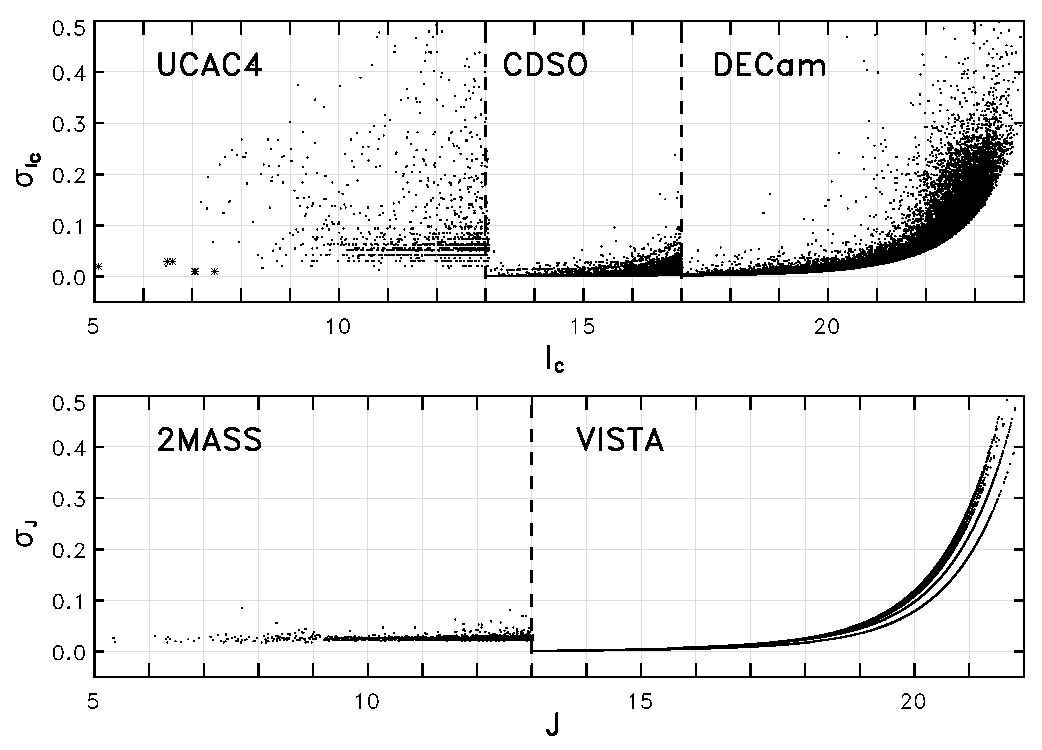
\includegraphics[width=1.00\textwidth]{f_3.pdf}
	\end{minipage} \hfill
	\begin{minipage}{0.35\textwidth}
		\caption[Photometric uncertainties of the catalogs used for the selection of member candidates.]{Photometric uncertainties as a function of magnitude for the merged optical (top) and NIR (bottom) catalogs. The labeled names indicate the catalogs used in each magnitude range separated by the dashed lines. The few $Hipparcos$ sources in the optical catalog are indicated by the asterisks.}
		\label{fig_IMF:errors}
	\end{minipage}
\end{figure}

For the control field approach, we estimated the field star contamination in our candidate sample by means of direct counting on selected regions as follows: $i)$ For the optical CDSO, UCAC4 and $Hipparcos$, and NIR 2MASS catalogs, we considered a control field of $1.0^\circ$ radius FOV placed at the same galactic latitude of 25 Ori in a direction moving away from the Orion's Belt ($\alpha_{J2000}= 05^{\rm h} 19^{\rm m} 03^{\rm s}.6$ and $\delta_{J2000} = +04^{\circ} 18' 17''.1$). $ii)$ Since we do not have neither DECam nor VISTA specific observations in this region, we used for these catalogs the areas of the eight north-westernmost and westernmost detectors of the DECam array as control fields, because a) they mostly lie outside the larger estimated area of 25 Ori, b) they have the lesser number of Orion OB1a reported members \citep{Briceno2018,Kounkel2018} and c) the density of LMS and BD candidates in the regions covered by these detectors falls to about 10\% of the density in the 25 Ori core \citep{Downes2014}. Then, we joined all the photometric catalogs from both control fields in the same way we did for the 25 Ori observations.

We applied our procedure for selecting photometric member candidates to the BGM and control field samples in order to account the sources lying inside the PMS locus, which we defined as contaminants. When we constructed the $I_c$ distributions of these contaminants in Section \ref{sec_IMF:LF}, we found consistency between the control field and the BGM for magnitudes brighter than $\sim 17$. In Table \ref{tab_IMF:candidates} we list the number of member candidates and contaminants after applying the spatial coverage corrections for the DECam data as well as their complete brightness and mass ranges. We estimated that the fraction of contaminants present in our candidate sample, in the $I_c$ brightness range between 13 and 20 mag, is about 30\%, which is somewhat higher than the 20\% estimated, and spectroscopically proven, by \citet{Downes2014} in the same brightness range for their candidate selection using similar CMDs. In Section \ref{sec_IMF:sample} we compared both samples. 

As mentioned in Section \ref{sec_IMF:locus} and shown in Figure \ref{fig_IMF:CMD}, there is a high contamination by giant and subgiant stars in the $I_c$ range between $\sim$9 and $\sim$13 mag in our candidate sample. Even, the contaminants estimated by the control field or the BGM can be as numerous as the member candidates in this particular brightness range, which do not allow us to remove the contamination in this range using only the control field or BGM. Fortunately, we can take advantage of Gaia DR2 because in this brightness range all sources have reliable parallaxes. Thus, we did a subset of the member candidates in this particular brightness range and having BJ18 distances around the 25 Ori distance and within a dispersion of 1-$\sigma$. From the candidate sample, there are about 600 sources with $I_c$ magnitudes between 9 and 13, of which 180 satisfy the distance criteria. Hereafter, we are going to refer to this subset of highly probable 25 Ori members as the distance filtered candidates.

After the correction for the DECam spatial coverage, we have only one BGM contaminant fainter than $I_c=19.6$ mag, while there are about 32 contaminants using the control field in the same brightness range. As the BGM does not include extragalactic sources, this difference between the contaminants counted in both samples suggests than most of the contamination present in the faintest range of our candidate sample is due to extragalactic sources. 

\begin{table}
%\centering\small
\caption[Number of member candidates and contaminants in our sample.]{Number, $I_c$ brightness and mass ranges of the member candidates and contaminants in an area of 1.1$^\circ$ radius in 25 Ori after correcting by the spatial coverage of the DECam data.}
	\small
	\label{tab_IMF:candidates}
    \setlength{\tabcolsep}{12pt}
	\begin{center}
 	\begin{tabular}{@{}lccc}
%	\multicolumn{3}{c}{ \normalsize {Sources Inside the Locus.}}\\
    \toprule
 	Origin  	       & Number            & $I_c$ range  & mass range \\ \vspace{-.05in}
					   & of sources        &              &            \\
 	    	   		   & 	        	   & (mag)        & ($M_\odot$)\\
    \midrule
 	25 Ori FOV         & 1782	  		   & 5.08-23.3    & 0.011-13.1   \\
 	Control Field FOV  & 1030 	  		   & 6.51-23.3    & 0.011-7.74     \\ 
 	BGM                & 840   	  		   & 7.67-19.6$^a$& 0.021$^a$-4.76 \\ 
    \bottomrule
 	\end{tabular}\\
	$^a$There is a fainter dwarf star contaminant with $I_c=23.5$ (0.011 $M_\odot$).
	\end{center}
\end{table}

\subsubsubsection{Contamination by Extragalactic Sources}
\label{sec_IMF:extgalcontam}
As 25 Ori is out of the galactic plane ($b=18.4^\circ$) and has a low extinction of 0.29$\pm$0.26 mag, we expect extragalactic sources in any deep photometric sample in that direction. We suggest in the previous section that the contamination by extragalactic sources dominates the contamination in the faintest range of our member candidate sample. To remove the most likely extragalactic sources from this sample we used the $J-K$ vs $Z-J$ color-color diagram shown in Figure \ref{fig_IMF:CCD}. We plotted a sample of $\approx 500$ spectroscopically confirmed galaxies and quasars in the direction of 25 Ori with $I_c$-brightness between 13.5 and 20.0 mag from \cite{Suarez2017}. Also, we plotted our member candidates and the previously confirmed members of 25 Ori. Similarly to what we did for the CMD, we defined the empirical isochrone traced by the low-mass and BD confirmed members. Then, we defined the sequence centered on this isochrone and containing over 90\% of the confirmed members. This sequence is clearly distinct from the region where are located more than $80$\% of the galaxies and quasars. About $1$\% (7 sources) of the member candidates plotted in this color-color diagram (those having VISTA photometry) lie in the region defined by the galaxy/quasar sample and have $I_c$ magnitudes between 15.2 and 18.2. We considered these 7 sources as contaminants and removed them from our member candidate sample, keeping the rest of the candidates selected in the CMD. The resultant sample has 1687 member candidates.

In Figure \ref{fig_IMF:CCD}, only four ($\sim$1\%) of the spectroscopically confirmed members lie in the region where most of the galaxies and quasars are located. Two of these peculiar members are classical T-Tauri stars (\ac{CTTS}s) harboring circumstellar disks and having an intense H$_\alpha$ emission \citep[41 and 53 \AA; ][]{Suarez2017}, while the other two have low H$_\alpha$ emission, one being a CTTS and the other one a weak T-Tauri star \citep[\ac{WTTS}; ][]{Briceno2007}. These four members are highly probable to be variable stars according to the CVSO, which could explain their position in the color-color diagram.

After we removed from our member candidate sample the potential extragalactic contaminants, we used the control field to statistically remove the extragalactic and galactic contamination from the LF and system IMF of 25 Ori in Section \ref{sec_IMF:LF} and \ref{sec_IMF:IMF}.

\begin{figure}[ht!]
	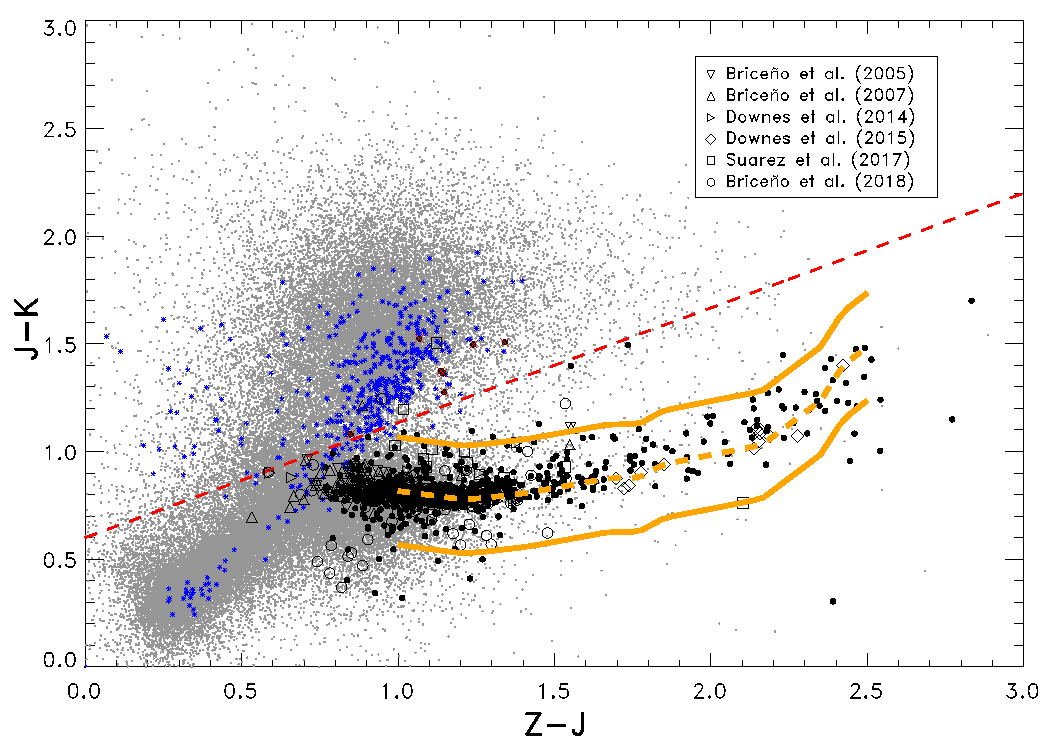
\includegraphics[width=1.00\textwidth]{f_4.pdf}
	\caption[$J-K$ vs $Z-J$ diagram to remove potential extragalactic sources in our candidate sample.]{Color-color diagram used to remove highly probable extragalactic contaminants (red crosses) from our member candidate sample (black dots). The blue asterisks represent a sample of spectroscopically confirmed galaxies and quasars in the direction of 25 Ori \citep{Suarez2017}. The red dashed line separates more than 80\% of the sample of extragalactic sources from the member candidates. The orange dashed curve shows the empirical isochrone traced by the low-mass and BD confirmed members of 25 Ori by the studies indicated in the label, which are mostly contained in the sequence defined by the orange solid curves. The gray dots are the same as in Figure \ref{fig_IMF:CMD}.}
	\label{fig_IMF:CCD}
\end{figure}

\subsubsubsection{IR excesses}
\label{sec_IMF:excesses}
Possible excesses in the $J$-band, due to disks, can bias the candidate selection because members showing such excesses could lie outside, on the red side, of the PMS locus. In Figure \ref{fig_IMF:CMD} there are 60 sources lying on the right side of the PMS locus, which have $I_c<12.7$ mag. The simulations performed with the BGM show that the positions of these sources are consistent with those of giant stars. Additionally, we checked the distances of these sources and compared them with the currently estimated 25 Ori distance. 97\% of the sources with reliable BJ18 distances have values not consistent with those of the 25 Ori members, of which most of them (91\%) have larger distances, suggesting these are, in fact, giant stars. Only two sources have distances consistent with 25 Ori, but these sources have unexpected photometric uncertainties from the UCAC4 catalog (0.146 and 0.234 mag), which could explain, in part, their location in the CMD. Thus, most of the sources left out, on the red side, of the PMS locus are behind the 25 Ori population, indicating that in our photometric selection we do not lose 25 Ori members due to the presence of IR excesses.

Additionally, if the magnitudes used to obtain the masses were affected by the IR excesses, the masses could be overestimated. However, at the age of 25 Ori, only a fraction of $\sim$5\% of the LMSs harbor circumstellar disks \citep{Briceno2005,Briceno2007,Hernandez2007a,Downes2014,Briceno2018}, which produce IR excesses starting at the $WISE\ 3.4\ \mu$m band or longer wavelengths \citep{Suarez2017}. Even for the BDs in 25 Ori, which have a larger disk fraction of $\sim 30$\%, the IR excesses start beyond the $H$-band \citep{Downes2015}. In this study we used the $I_c$ and $J$-band magnitudes which are not expected to be affected by IR excesses. In any event, we worked with the $I_c$ magnitudes to estimate masses to avoid any overestimation due to IR excesses.

\subsubsubsection{Effects of Chromospheric Activity}
\label{sec_IMF:activity}

Active LMSs suppress the effective temperature (\ac{Teff}) by $\sim5$\% and inflate the radius by $\sim10$\% with respect to inactive objects \citep[e.g. ][]{Lopez-Morales2007}. These effects roughly cancel themselves, which preserves the bolometric luminosity \citep{Stassun2012}. 

Due to the effective temperature suppression, the masses of active LMSs estimated from the Hertzsprung-Russell (\ac{H-R}) diagram are underestimated, but if masses are estimated from luminosities (or absolute magnitudes), the effect would be much smaller \citep{Jeffries2017}. According to \citet{Stassun2012}, when the effective temperature is used to estimate masses from model isochrones, the resultant masses are systematically lower than the true masses by factors of $\sim3$ and $\sim2$ for LMSs and BDs with intense chromospheric activity of log($L_{H_\alpha}/L_{bol})=-3.3$, respectively. This level of chromospheric activity corresponds to the saturation limit in young LMSs, which separates the CTTSs from WTTSs \citep{BarradoYNavascues-Martin2003}. For LMSs and BDs with low levels of magnetic activity (log($L_{H_\alpha}/L_{bol})=-4.5$), the masses estimated using the effective temperature are systematically lower than true values by factors of $\sim2$ and $\sim1.5$, respectively. Instead, when masses are estimated using the bolometric luminosity derived from the $K$-band absolute magnitudes and considering model isochrones, the resulting masses are $\sim5$\% smaller than true values for LMSs and BDs with high chromospheric activity and roughly unaffected for LMSs and BDs with low chromospheric activity.

In our case, as explained in Section \ref{sec_IMF:mass-luminosity}, we obtained the masses of the member candidates using absolute magnitudes and model isochrones, which minimize the bias in the mass determination of active stars. Additionally, the fraction of active stars in 25 Ori is $\sim 5$\% \citep[][]{Briceno2005,Briceno2007,Hernandez2007a,Downes2014,Briceno2018}. Considering the expected $\sim$5\% underestimation of masses for the expected $\sim$5\% of active stars in our candidate sample, we estimated that the change in the system IMF of 25 Ori is smaller than the Poisson noise of the distribution.

\subsubsubsection{Spatial Resolution and Binaries}
Most of the mass distributions of stellar clusters available in the literature do not take into account unresolved binaries or multiple systems and are, in fact, the system IMFs \citep[e.g. Table \ref{tab_IMF:imf_literature} and ][]{Bastian2010}.

A revision and treatment of the effect of unresolved binary systems in the IMF parameterization is found in \citet{Muzic2017}. They found that the mass distribution becomes steeper in the low-mass and high-mass sides when correcting the system IMF by binary systems to obtain the single-star IMF, but the changes in the slopes agree within the uncertainties. A similar effect on the IMF due to binary systems is reported in \citet{Kroupa2001b}.

In this study we reported the system IMF of 25 Ori, which will allow us to directly compare it with all the system IMFs in Table \ref{tab_IMF:imf_literature}, assuming that the binarity properties are similar for these populations and a similar spatial resolutions of the data used in the different studies. The conversion of the 25 Ori system IMF to the single-star IMF is beyond the scope of this study.

\subsubsubsection{Estimation of the Missed Members}
\label{sec_IMF:missed}
As explained in previous sections, in our estimation of the system IMF we corrected the possible over-counting of individual stars and/or stellar systems belonging to 25 Ori by considering several sources of contamination in the photometric sample. An additional improvement of our procedure is to estimate possible under-counting of members by estimating the number of 25 Ori individual stars and/or stellar systems that could lie outside the PMS locus defined in the CMD.

We made this estimation through a simple simulation of the expected distribution of the cluster members in the $I_c$ vs $I_c-J$ diagram and computing the fraction of these that falls outside the PMS locus. The simulation was performed as follows, in which we refer as \emph{synthetic members} to those individual stars and/or stellar systems obtained from a realization of the system IMF:

$(i)$ We made a random realization of the 25 Ori system IMF by drawing masses for 1700 synthetic members from a lognormal distribution with $m_c=0.31$ and $\sigma=0.46$. These parameters matches the number of 25 Ori candidates in our sample as well as the resulting system IMF that will be discussed in Section \ref{sec_IMF:parameterizations}. 

$(ii)$ The $I_c$ and $J$-band absolute magnitudes of each synthetic member were computed by interpolating their masses into the mass-luminosity relation using the 7 Myr isochrones of BT-Settl and PARSEC-COLIBRI, as explained in Section \ref{sec_IMF:mass-luminosity}.

$(iii)$ The absolute magnitudes were converted into apparent magnitudes by adding the distance moduli and the corresponding extinctions. The distances and extinctions were generated for each synthetic member by creating random realizations considering the inversion of the cumulative distributions of the BJ18 distances and visual extinctions from spectroscopically confirmed members of 25 Ori (see Figure \ref{fig_IMF:cum_dist}). Visual extinctions were converted into extinctions in $I_c$ and $J$ bands through the \cite{Rieke-Lebofsky1985} extinction law with $R_V$=3.02.

$(iv)$ We randomly labeled $25$\% of the synthetic members as photometrically variables in both $I_c$ and $J$ bands. To each of the variables we assigned a variation, $\Delta I_c$, drawn at random from a normal distribution with zero mean and standard deviation, $\sigma _{I_c}$, equal to 0.3. The fraction of variables as well as $\sigma _{I_c}$ were obtained by matching the catalog of member candidates with the CVSO, which includes stars and BDs with K and M spectral types. A total of 840 candidates ($\sim$50\% of the candidate sample) fainter than $I_c=13$ mag (saturation of the CVSO) have a counterpart in the CVSO and we considered as variable the 220 candidates having a probability $>99$\% of being variables in the $I_c$-band. The $J$-band variation was computed by multiplying the $\Delta I_c$ by the ratio between the amplitude variations in the $I_c$ and $J$-bands from \cite{Scholz2009}. Both variations were added to the corresponding apparent magnitudes computed in $(iii)$.

$(v)$ We assumed no IR excesses in the $J$-band because at the 25 Ori age they are observed at larger wavelengths, as explained in Section \ref{sec_IMF:excesses}.

$(vi)$ Finally, we simulated the photometric uncertainties in the $I_c$ and $J$-bands by adding to the corresponding apparent magnitude a random error based on an estimation of the photometric errors present in our data. Such estimations were obtained through the fit we did to the mean errors as a function of the mean magnitudes and a fit of the standard deviation of errors as a function of the mean magnitude. Then, for each source, the final apparent magnitude is computed by extracting a magnitude from a normal distribution which is centered at the mean apparent magnitude resulting from $(v)$ with a standard deviation equal to the standard deviation of errors that corresponds to such mean apparent magnitude.

We generated 1000 random realizations of the cluster and obtained that a mean fraction of $\sim3.1$\% of the synthetic members fall outside the PMS locus, with most of them ($\sim3.0$\%) lying on the left side. We found that this fraction and distribution are consistent with the fraction of confirmed members lying outside the PMS locus shown in Figure \ref{fig_IMF:CMD}. In Figure \ref{fig_IMF:syntheticIvsIJ} we show the result of a characteristic simulation.

Through the variation of the input parameters within values representative of 25 Ori, we found that the main effects that can move synthetic members outside the PMS locus is the photometric variability. As expected, within reasonable values, the system IMF parameters $m_c$ and $\sigma$ do not affect the number of synthetic members falling outside the PMS locus, so our estimation of the under-counting is not affected by the assumed system IMF.

\begin{figure}[ht!]
	\begin{minipage}{0.60\textwidth}
		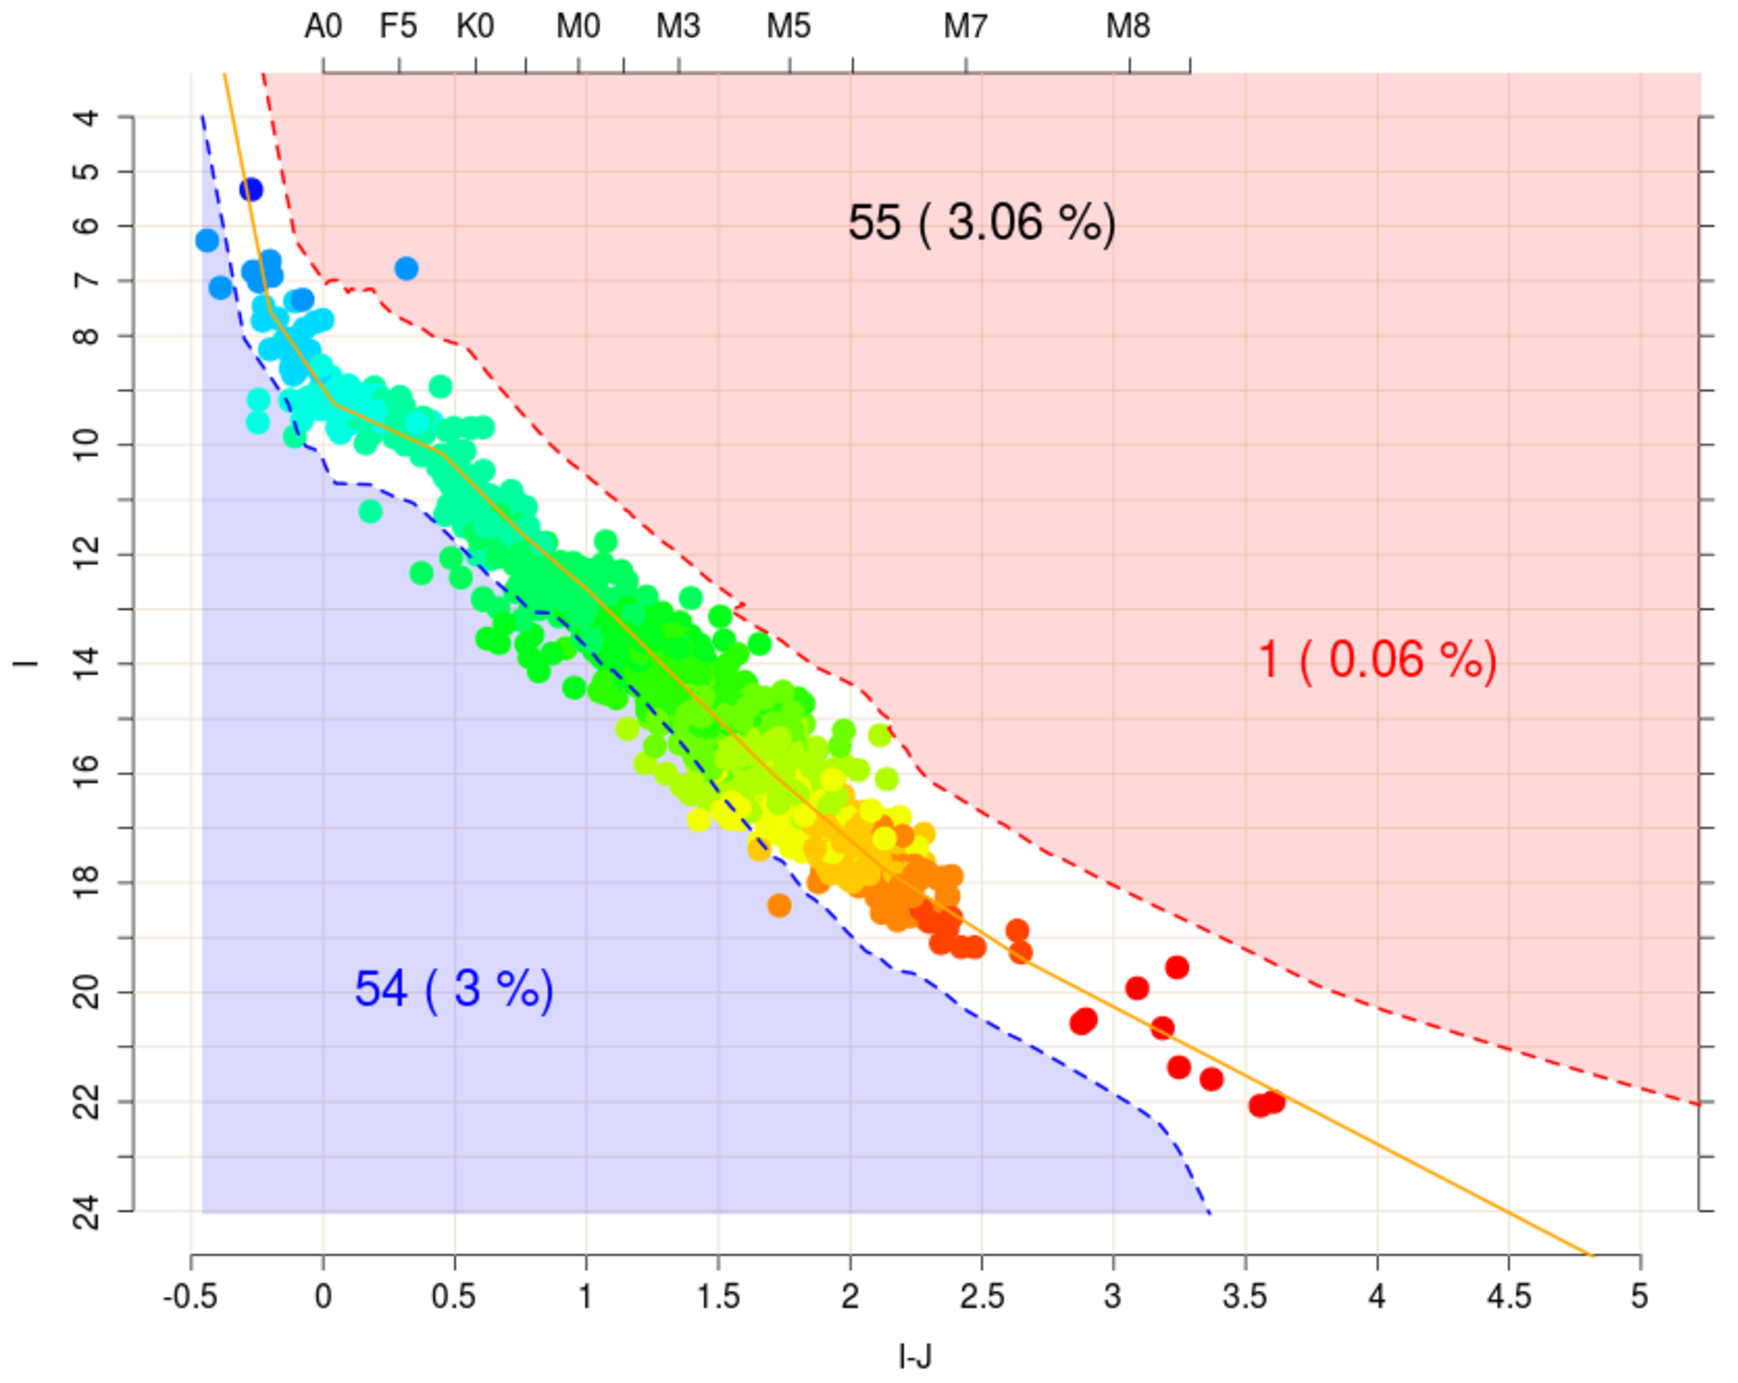
\includegraphics[width=1.00\textwidth]{f_5.pdf}
	\end{minipage} \hfill
	\begin{minipage}{0.35\textwidth}
		\caption[Simulated $I_c$ vs $I_c-J$ diagram to estimate missed members in our sample.]{Simulated $I_c$ vs $I_c-J$ diagram for the estimation of the number of members missed by our candidate selection procedure. Dashed lines indicate the PMS locus and solid line the empiric isochrone. The number and fraction in the top of the plot indicate the missed members in both sides of the PMS locus, as indicated in the labels, considering the 1700 synthetic members. The colored scale indicates the mass of the synthetic members.
		\label{fig_IMF:syntheticIvsIJ}}
	\end{minipage}
\end{figure}

\subsubsection{Resulting Sample of Member Candidates}
\label{sec_IMF:sample}
The resultant sample selected from the PMS locus in the CMD and after removing potential extragalactic contaminants in the color-color diagram has 1687 photometric member candidates with $I_c$ magnitudes between 5.08 and 23.3 ($0.011-13.1\ M_\odot$) and covering an area of 1.1$^\circ$ radius in 25 Ori. The completeness of this sample is at $I_c=22.5$ mag ($12\ M_{Jup}$) and the brightest sources in 25 Ori are also included. For a statistical removal of the field star and extragalactic contaminants in this sample, when constructing the LF and system IMF in Sections \ref{sec_IMF:LF} and \ref{sec_IMF:sys-imf}, respectively, we used the control field and, as a comparison for the galactic contamination, the BGM. The contamination present in our sample depends of the brightness range but it can be roughly characterized into three ranges. The extragalactic contamination starts to be significant for $I_c$ magnitudes fainter than $\sim$17 mag. For the bright $I_c$ range, between $\sim$9 to 13 mag, there is a high level of contamination by giant and subgiant stars (reason why we did a subset of the sample filtered in distance). In the brightness range between these kind of contaminants, the PMS population is clearly distinguished from the old dwarf stars and the contamination decreases. We estimated, using the control field and/or the BGM, a contamination of $\sim20$\% in our sample in the range between 13 and 17 mag. Actually, in this brightness range is where most of the 25 Ori members has been spectroscopically confirmed, as show in Figure \ref{fig_IMF:CMD}.

With our sample we confirmed the low density in 25 Ori. We obtained a stellar density of 8.6 to 4.8 stars/pc$^3$ for the areas of 0.5 and 1.0$^\circ$ radius, respectively, while the substellar density ranges from 1.3 to 0.7 BDs/pc$^3$ for the same areas, considering the 25 Ori distance estimated in this study. This stellar density values are roughly consistent with \citet{Briceno2007,Downes2014,Briceno2018}.

We compared our candidate sample with the candidate selection done by \citet{Downes2014} using a similar procedure and the CDSO and VISTA catalogs. Their sample includes candidates with masses in a smaller range ($0.02\le M/M_\odot\le0.80$) but covering a larger area (about 3x3 deg$^2$ around 25 Ori). If we consider the same area as in the present work, there are about 750 candidates in their selection. Our sample contains 924 member candidates in the same mass range and includes 91\% of their candidates. More than a half of their candidates not included in our sample and with $I_c>17$ mag (brightness limit from which we used the DECam photometry) lie within the gaps of the DECam array. Thus, where we have full spatial coverage, we recover more than 96\% of the member candidates by \citet{Downes2014} and, additionally, we reported 242 new candidates in the same mass range covered by their study. We estimated that the contamination in our candidate sample, in the $I_c$ brightness range between 13 to 20 mag, is about 30\%, which is somewhat higher than the 20\% estimated and spectroscopically proven by them in their sample. This difference is due, mainly, because our PMS locus is somewhat wider.

\subsection{Results and Discussion}
\label{sec_IMF:results}

\subsubsection{Luminosity Function}
\label{sec_IMF:LF}
In order to construct the LF we calculated the absolute magnitudes of the member candidates and contaminants considering they are real members of 25 Ori. This consideration allow us to analyze properties of the candidate sample as a whole, such as the LF and the system IMF after correcting the effect of the contamination.

The absolute magnitudes were obtained using our joined $I_c$-band catalog and, as only 18\% of the candidates (those spectroscopically confirmed as members) have extinctions from previous studies and 86\% of the sample has reliable BJ18 distances, we assigned distance and extinction values to the whole sample as follow: From a list of 334 spectroscopically confirmed members of 25 Ori \citep{Briceno2005,Briceno2007,Downes2014,Downes2015,Suarez2017,Briceno2018}, we constructed the normalized cumulative distributions of their BJ18 distances and reported extinctions. Then, we used the inversion of these observed distributions to create random realizations to assign values of these parameters to each member candidate, even those already having reliable Gaia DR2 parallaxes or extinctions from previous spectroscopic studies in order to have a sample with all values consistent with those from the 25 Ori members. A detailed explanation of this procedure is found in Appendix \ref{sec_app_IMF:distance_extinction}. With these distances and extinctions, together with the $I_c$ photometry, we computed the corresponding absolute magnitudes, $M_{I_c}$, for all the member candidates. We made $10^4$ repetitions of this experiment in order to obtain a robust simulation, which produced $10^4$ artificial distributions in the $M_{I_c}$ range from -2.8 to 15.4 mag.

In a similar way we obtained $10^4$ $M_{I_c}$ magnitudes for each candidate in the distance filtered subset. The resultant $M_{I_c}$ range of this subset is between $\sim 1$ and $\sim 5$ mag, assuming the distance and extinction of 25 Ori, and corresponds to the region mostly affected by giant and subgiant stars.

For the contaminants from the control field and BGM, we estimated their fiducial $M_{I_c}$ magnitudes following the same procedure we used for the member candidates. This way, we can estimate the contamination in the $M_{I_c}$ distribution of the member candidates to then obtain the LF.

Using the simulation just described, we constructed the $10^4$ $M_{I_c}$ distributions of the member candidate and contaminant samples. To correct each distribution by the DECam spatial coverage factor explained in Section \ref{sec_IMF:spatial}, we first made the $M_{I_c}$ distributions of the sources from the DECam catalog and applied them the correction. Then, we added to these distributions those from the rest of the data.

With the $10^4$ $M_{I_c}$ distributions of the member candidate sample, we defined the distribution using the mean values and assigning uncertainties of 1 $\sigma$. Similarly, we defined the distribution of mean values for the contaminants. The resultant distribution of the contaminants from the control field and the BGM are consistent within the uncertainties for $M_{I_c}$ magnitudes brighter than $\sim 9$, even where the giant and subgiant stars lie, which indicates that the contamination in our sample in this range is due mainly to field stars. For fainter sources, a significant discrepancy arises between both samples of contaminants, which increases with the magnitude, suggesting the presence of extragalactic sources. We decided to work with the contaminants estimated from the control field because this also allow us to remove these extragalactic sources.

To the $M_{I_c}$ distribution of the member candidates we subtracted the distribution of the contaminants from the control field and by adding the errors in quadrature. In the resultant distribution we replaced the $M_{I_c}$ interval ($\sim1-5$ mag) containing a high giant and subgiant star contamination by the distribution of the candidates in the distance filtered subset, which results in the LF of 25 Ori.

We constructed LFs for different FOVs starting with a radius of $1.1^\circ$ and decreasing it by steps of $0.1^\circ$ until having a radius of $0.5^\circ$ (the 25 Ori overdensity). In Figure \ref{fig_IMF:LF} we show the LFs for the 25 Ori estimated areas. These LFs have very similar morphologies, within the uncertainties.

\begin{figure*}[ht!]
	\centering
	\begin{tabular}{ccc}
		\subfloat{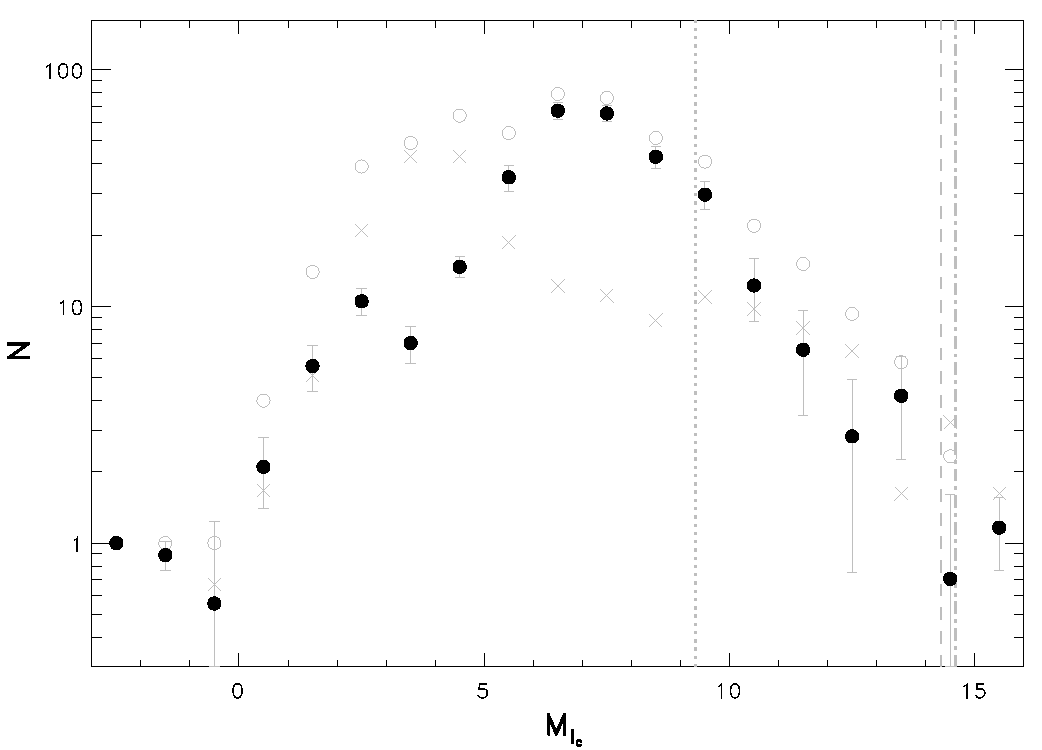
\includegraphics[width=.33\linewidth]{f_6-1.pdf}} & 
		\subfloat{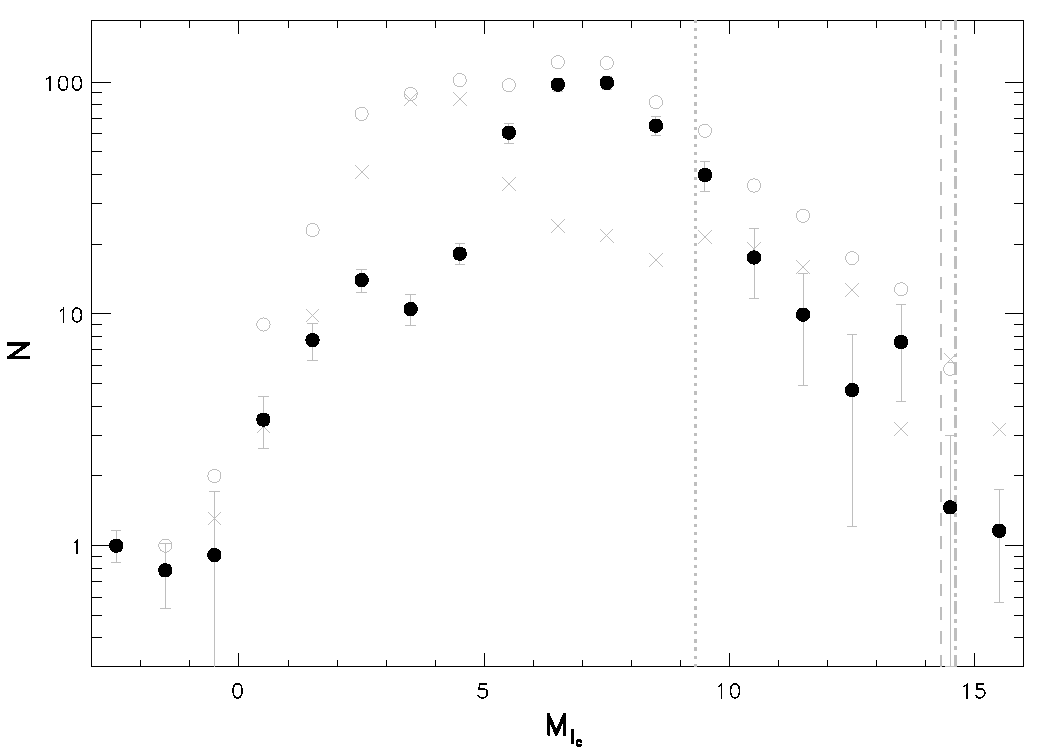
\includegraphics[width=.33\linewidth]{f_6-2.pdf}} &
		\subfloat{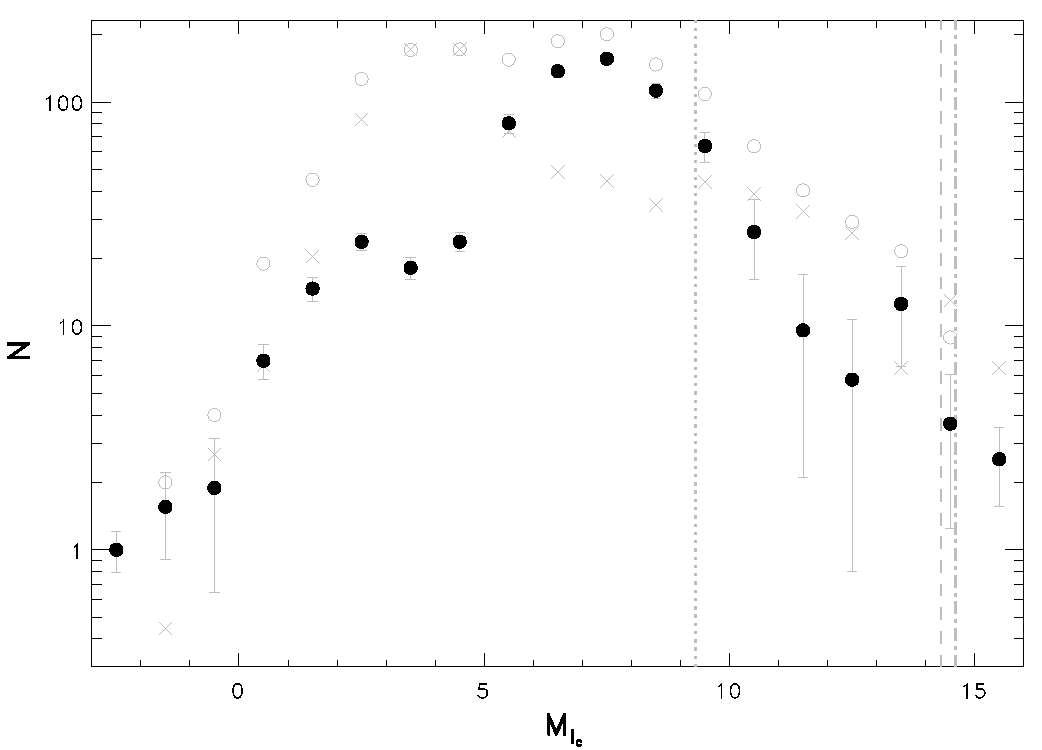
\includegraphics[width=.33\linewidth]{f_6-3.pdf}}
	\end{tabular}
	\caption[LFs for the 25 Ori areas.]{LFs after correcting by the galactic and extragalactic contamination (gray crosses) in our member candidate sample (gray open circles) inside the 25 Ori estimated areas. The panels from left to right correspond to the areas by \citet[0.5$^\circ$ radius; ][]{Downes2014}, \citet[0.7$^\circ$ radius; ][]{Briceno2018} and \citet[1.0$^\circ$ radius; ][]{Briceno2005,Briceno2007}. The vertical lines, from left to right, indicate the substellar limit (H burning limit), the BD-planetary object limit (D burning limit) and the completeness limit of our DECam observations.
	\label{fig_IMF:LF}}
\end{figure*}

\subsubsection{System IMF}
\label{sec_IMF:IMF}
The main purpose of this study is to determine the system IMF of 25 Ori. Therefore, we need to estimate through a mass-luminosity relationship, the corresponding masses for our member candidates and contaminants under the consideration that both are true members of 25 Ori.

\subsubsubsection{Mass-Luminosity Relationship}
\label{sec_IMF:mass-luminosity}
At the age of 25 Ori \citep[7-10 Myr; ][]{Briceno2005,Briceno2007,Downes2014,Briceno2018}, stars with masses between $\sim 2$ and $\sim 15\ M_\odot$ should be already in the MS, while less massive objects are still in the PMS and more massive stars are in post-MS stages \citep[][]{Prialnik2000}. The most massive star in 25 Ori is the star with the same name, classified as a peculiar B1V star with broad lines \citep{Houk1999}, which roughly corresponds to $\sim 10\ M_\odot$ using the \citet{Schmidt-Kaler1982} empirical mass-luminosity relationship. Therefore, we do not expect in our candidate sample members of 25 Ori being in post-MS but we do expect PMS and MS members. We estimated that $\sim7$\% of our candidates have masses larger than 2 $M_\odot$, considering the system IMF by \citet{Downes2014}.

In order to cover the large $M_{I_c}$ range in our candidate sample (from -2.8 to 15.4 mag), we worked with two sets of mass-luminosity relationships for PMS and MS stellar models at the age of 25 Ori. We considered the 7 Myr isochrones of PARSEC-COLIBRI for masses higher than $1.0\ M_\odot$ and of BT-Settl for lower masses. These isochrones were obtained assuming solar metallicity. In Figure \ref{fig_IMF:mass-L} we show the resulting mass-luminosity relation from high-mass stars to very low-mass objects (from 0.01 to 15 $M_\odot$). We stress the soft transition between both isochrones at the selected cutoff at 1$M_\odot$. 

\begin{figure}[ht!]
	\begin{minipage}{0.60\textwidth}
		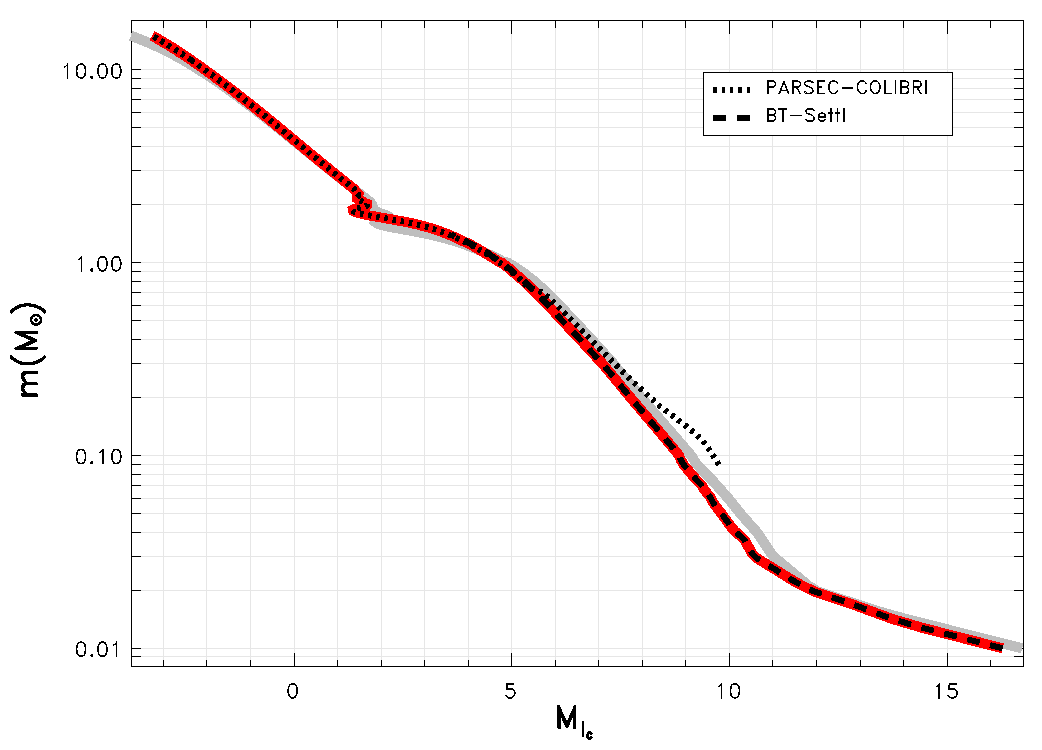
\includegraphics[width=1.00\textwidth]{f_7.pdf}
	\end{minipage} \hfill
	\begin{minipage}{0.38\textwidth}
		\caption[Mass-luminosity relation for estimating masses.]{Mass-luminosity relation used to estimate the masses of the member candidates and contaminants (red solid curve). This relation is a combination of the 7 Myr isochrones of BT-Settl and PARSEC-COLIBRI, which are indicated by the dashed curve and the dotted curve, respectively. As a reference, the mass-luminosity relation considering instead the 10 Myr isochrones is represented by the gray solid curve, which is mostly contained into the thickness of the mass-luminosity relation for 7 Myr.}
		\label{fig_IMF:mass-L}
	\end{minipage}
\end{figure}

\subsubsubsection{System IMF Determination}
\label{sec_IMF:sys-imf}
By interpolation of the $M_{I_c}$ magnitudes into the mass-luminosity relationship explained in the previous section, we estimated the masses that correspond to each member candidate as well as to each contaminant considering they are members of 25 Ori. As we have $10^4$ $M_{I_c}$ values for each source, we obtained $10^4$ masses for each source. The resulting mass range covered by the member candidates is between $0.011$ and 13.1 $M_\odot$. In Table \ref{tab_IMF:candidates} we list this mass range along with those for the samples of contaminants.

With these masses we constructed the mass distributions of the member candidates and contaminants. Similarly than for the $M_{I_c}$ distributions, we corrected the distributions by the spatial completeness of DECam and then we defined the mass distribution using the mean values and assigning errors of 1 $\sigma$. From the mass distribution of the member candidates we subtracted that of the control field contaminants adding the errors in quadrature. Then, we replaced in the resulting distribution the range between $\sim$0.9 and 3 $M_\odot$ by the mass distribution of the candidates in the distance filtered subset. The resultant distribution corresponds to the system IMF of 25 Ori, which is complete from 12 $M_{Jup}$ to 13.1 $M_\odot$ (corresponding to the 25 Ori star).

In Figure \ref{fig_IMF:imf} we show the system IMFs for the 25 Ori estimated areas. The least massive bin (at log $m=-1.9$) is partially affected by the completeness of our DECam data in the magnitude range between 21 and 24 mag. Then, we corrected the counts in these magnitude range by a factor of $\sim2.5$, which results from the ratio between the expected number sources (from extrapolation of the magnitude distribution) and those observed in this DECam magnitude range.

\begin{figure*}[ht!]
	\centering
	\begin{tabular}{ccc}
		\subfloat{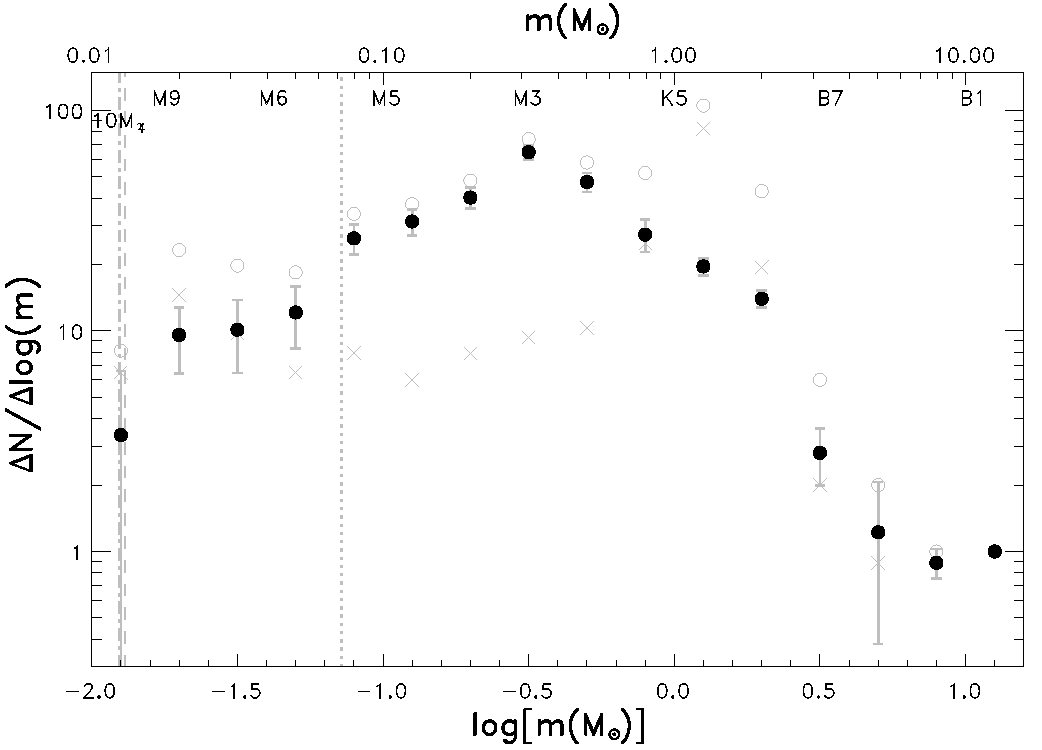
\includegraphics[width=.33\linewidth]{f_8-1.pdf}} & 
		\subfloat{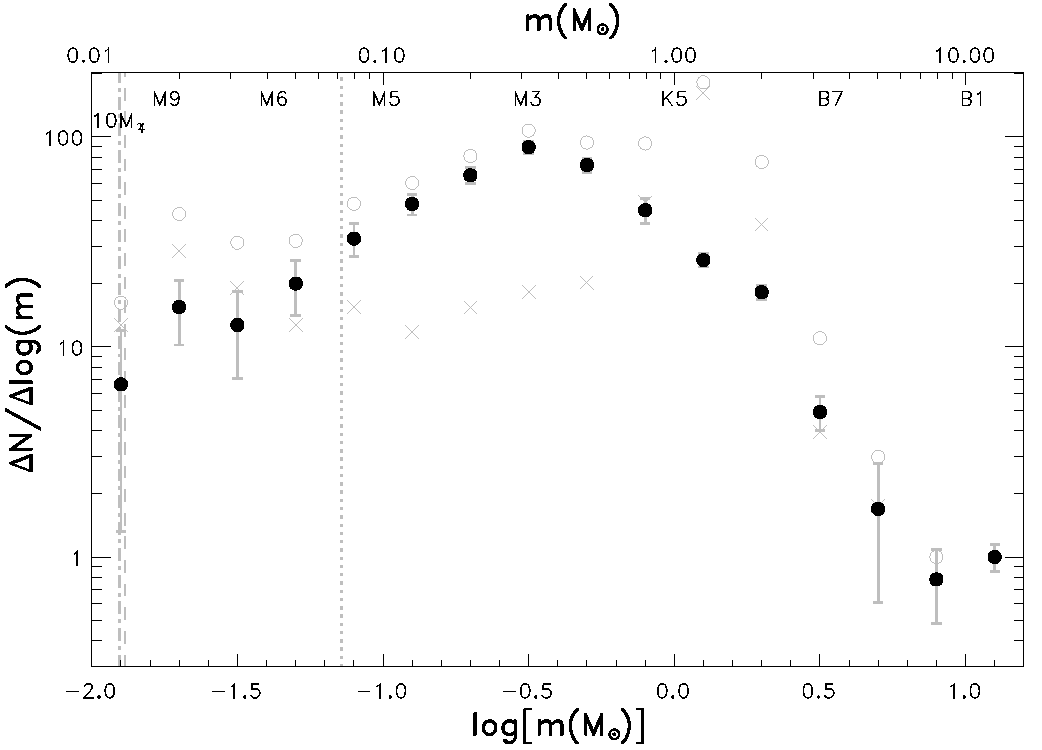
\includegraphics[width=.33\linewidth]{f_8-2.pdf}} &
		\subfloat{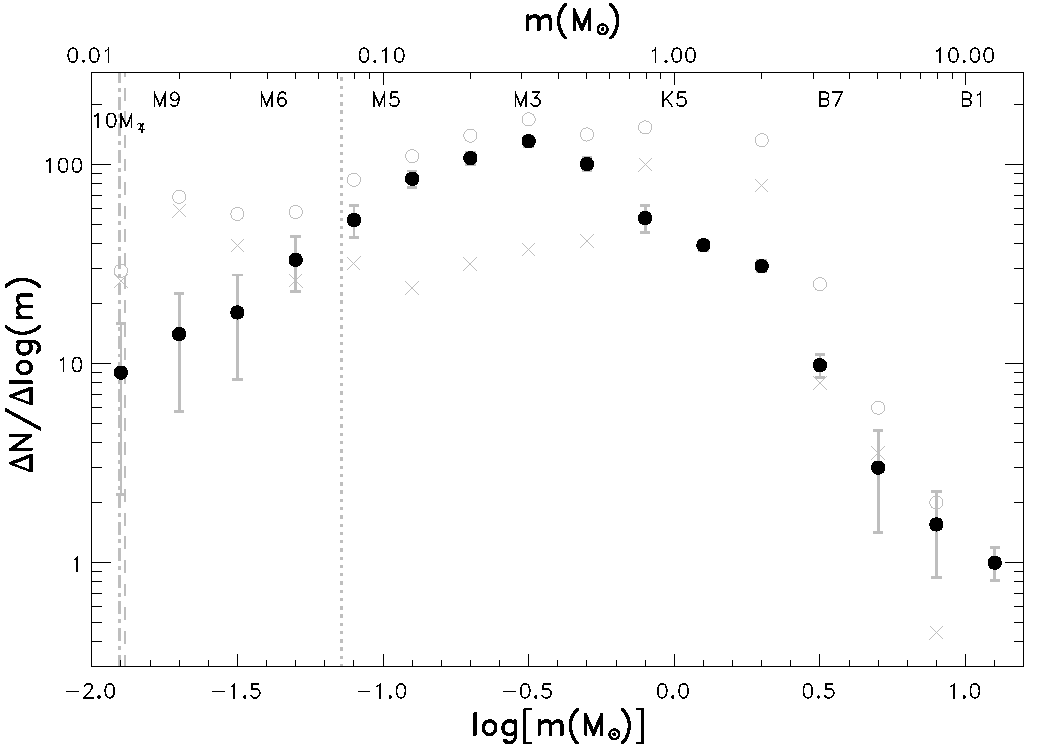
\includegraphics[width=.33\linewidth]{f_8-3.pdf}} 
	\end{tabular}
	\caption[25 Ori system IMFs]{System IMFs of 25 Ori after correcting by the galactic and extragalactic contamination (gray crosses) in our member candidate sample (gray open circles). The panels, from left to right, correspond to the 25 Ori areas by \citet[0.5$^\circ$ radius; ][]{Downes2014}, \citet[0.7$^\circ$ radius; ][]{Briceno2018} and \citet[1.0$^\circ$ radius; ][]{Briceno2005,Briceno2007}. The vertical lines are the same as in Figure \ref{fig_IMF:LF}. The spectral type scale is from \citet{Pecaut2013}. The size of the bin is 0.2 dex.
	\label{fig_IMF:imf}}
\end{figure*}

\subsubsubsection{Parameterizations}
\label{sec_IMF:parameterizations}
We described the derived system IMF of 25 Ori using the following parameterizations:

$i)$ A three-part power-law distribution in the form:

\begin{equation}
	\xi(\log m)\propto m^{-\Gamma_i}
\end{equation}

with $\Gamma_1$, $\Gamma_2$ and $\Gamma_3$ for the mass ranges $m\le0.30\ M_\odot$, $0.30<m/M_\odot<1$ and $m\ge1\ M_\odot$, respectively. Such parameterization is inspired by that for the Galactic-field IMF proposed by \citet{Kroupa2001b,Kroupa2002}, but with different break masses because his IMF is defined when resolving multiple systems.

$ii)$ A lognormal distribution for masses $m\le1M_\odot$, according to \citet{Chabrier2003a,Chabrier2003b}:

\begin{equation}
\xi(\log m)\propto e^{-\frac{(\log m-\log m_c)^2}{2\sigma^2}}
\end{equation}

where $m_c$ is the characteristic mass and $\sigma$ the standard deviation. If we consider the lognormal fit up to 13.1 $M_\odot$, the resultant parameters are in agreement, within the errors, with those when the fit is done for masses $m\le1M_\odot$.

$iii)$ A tapered power-law function for the whole mass range of the system IMF ($0.012-13.1\ M_\odot$):

\begin{equation}
\xi(\log m)\propto m^{-\Gamma} \Big[1-e^{-(m/m_p)^\beta}\Big]
\end{equation}

where $m_p$ is the peak mass, $\Gamma$ the power law index and $\beta$ the tapering exponent. This function, introduced by \citet{DeMarchi2005}, has a power law behavior for high masses and an exponential truncation for lower masses.

In Figure \ref{fig_IMF:imf_par} we show these functions fitted to the 25 Ori system IMF and in Table \ref{tab_IMF:imf} we summarize the parameters with their uncertainties. In these fits we avoided the most massive bin(s) with counts lesser than the unity because they are at the noise level. The reason why we have counts lesser than one is because to the member candidate mass distribution we subtracted the mass distribution of the contaminants after applying the correction by the spatial coverage, which can result in a fractional number.

\begin{figure*}[ht!]
	\centering
	\begin{tabular}{ccccccccc}
		\subfloat{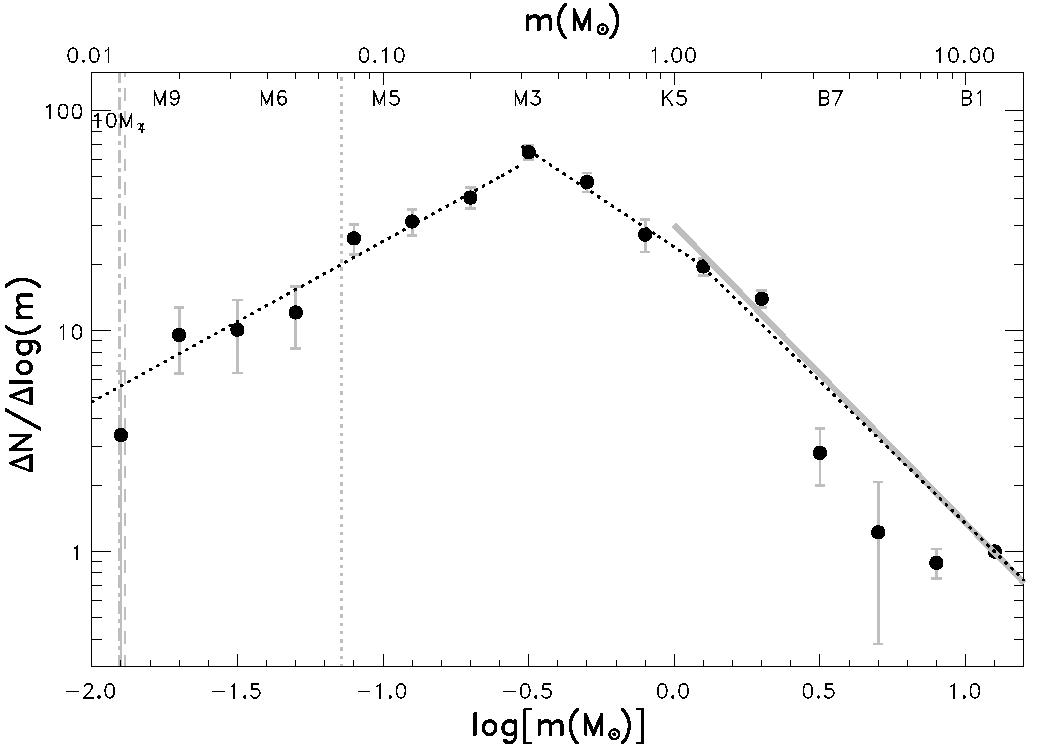
\includegraphics[width=.33\linewidth]{f_9-1.pdf}} & 
		\subfloat{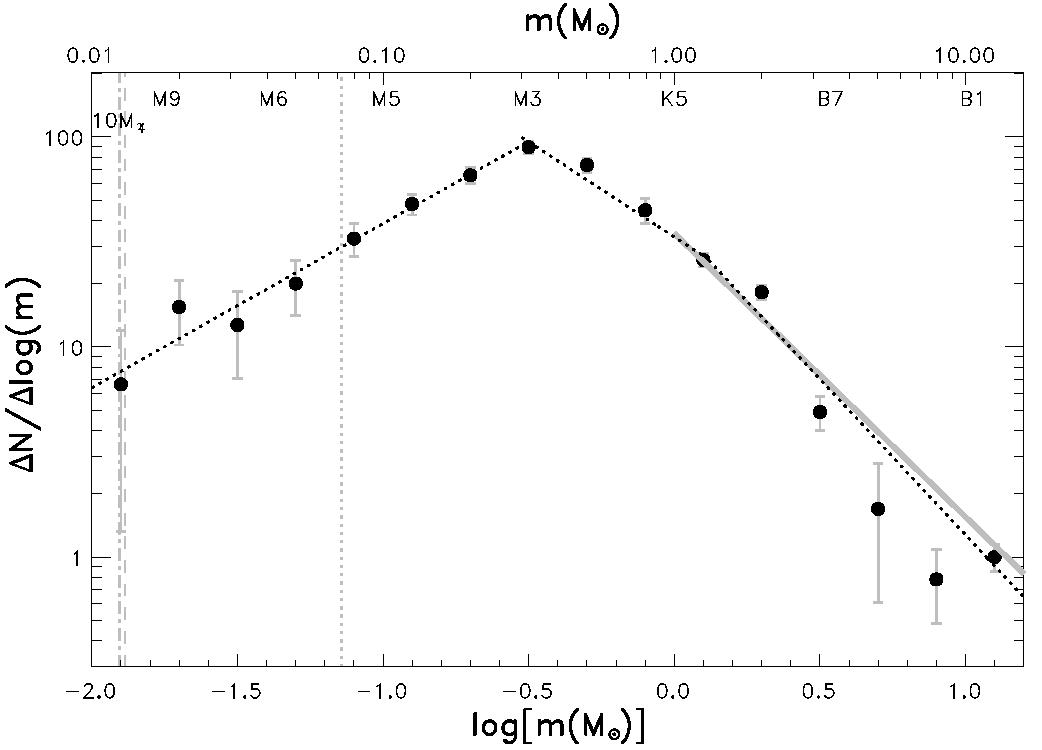
\includegraphics[width=.33\linewidth]{f_9-2.pdf}} &
		\subfloat{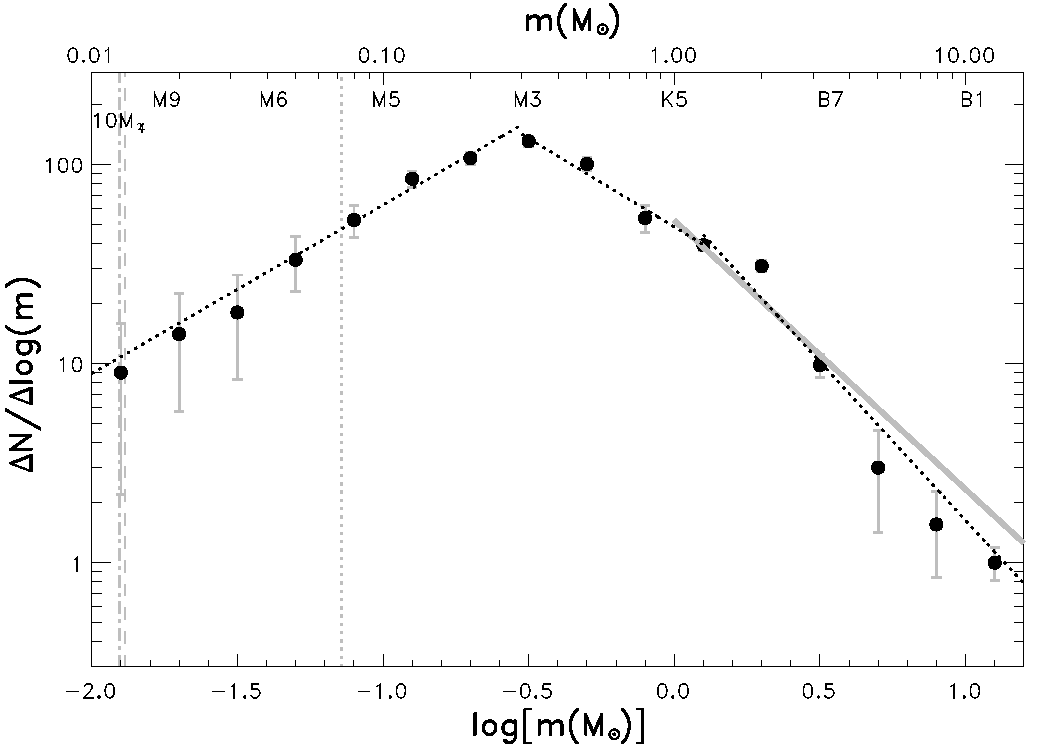
\includegraphics[width=.33\linewidth]{f_9-3.pdf}} & \\
		\subfloat{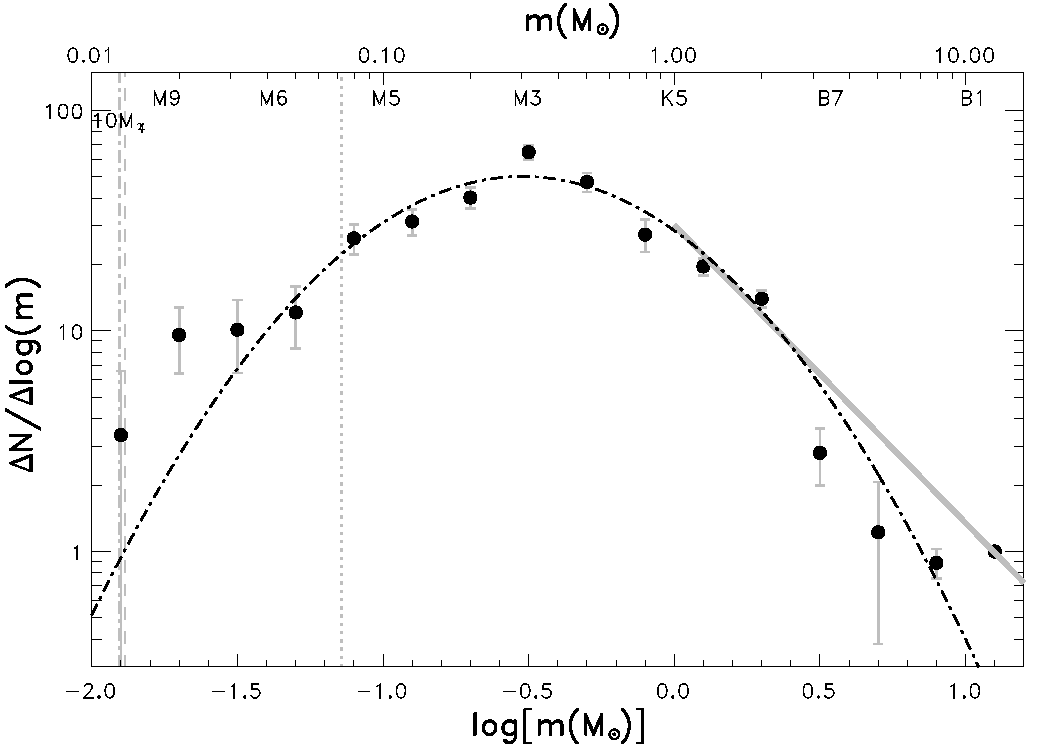
\includegraphics[width=.33\linewidth]{f_9-4.pdf}} & 
		\subfloat{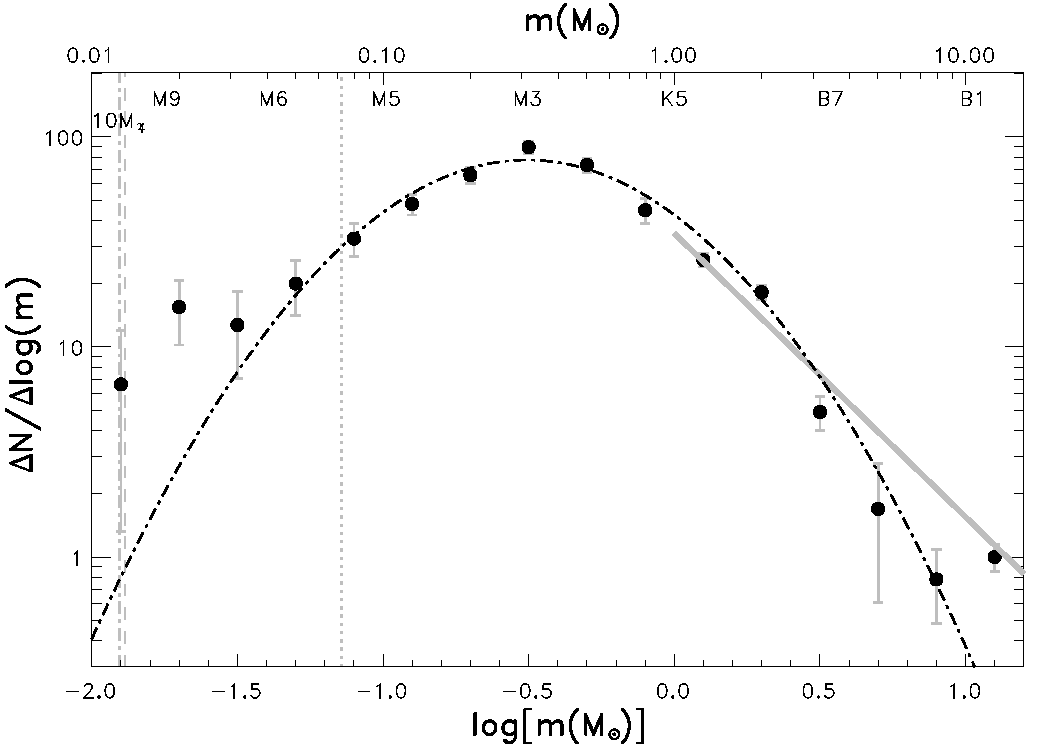
\includegraphics[width=.33\linewidth]{f_9-5.pdf}} &
		\subfloat{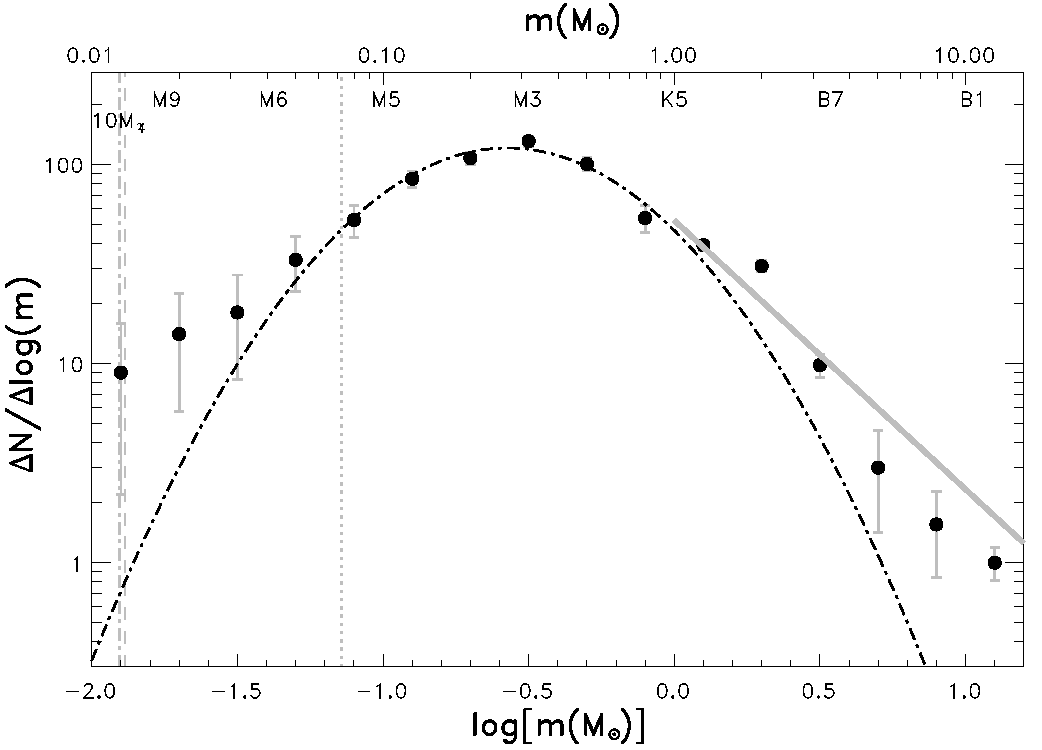
\includegraphics[width=.33\linewidth]{f_9-6.pdf}} & \\
		\subfloat{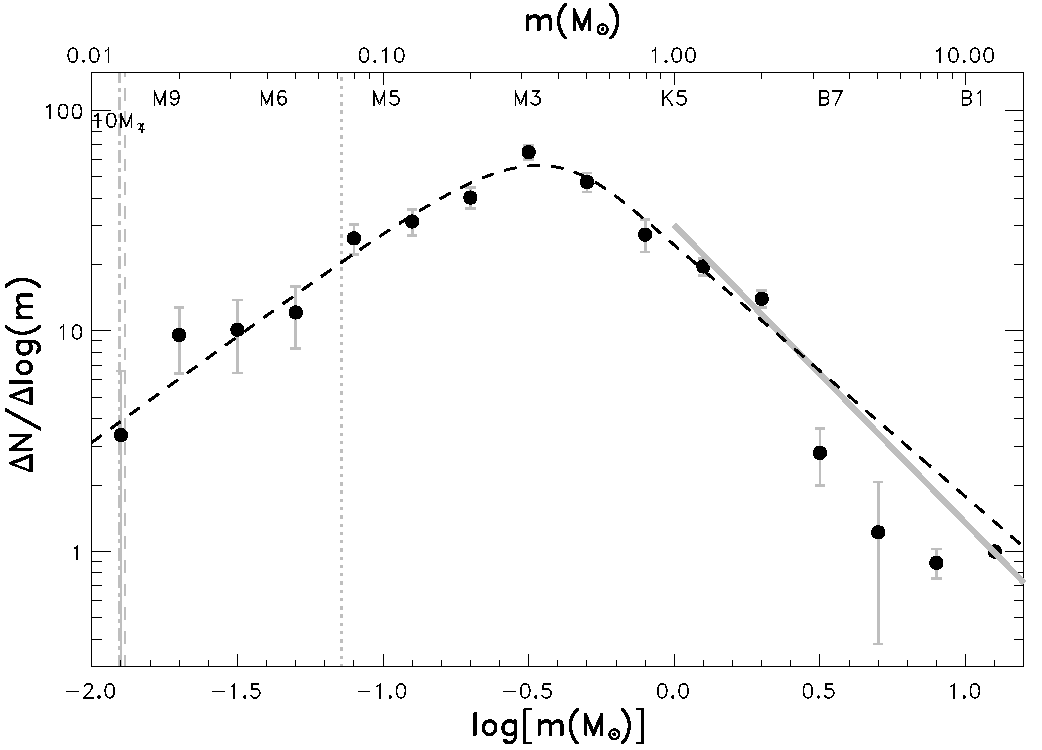
\includegraphics[width=.33\linewidth]{f_9-7.pdf}} & 
		\subfloat{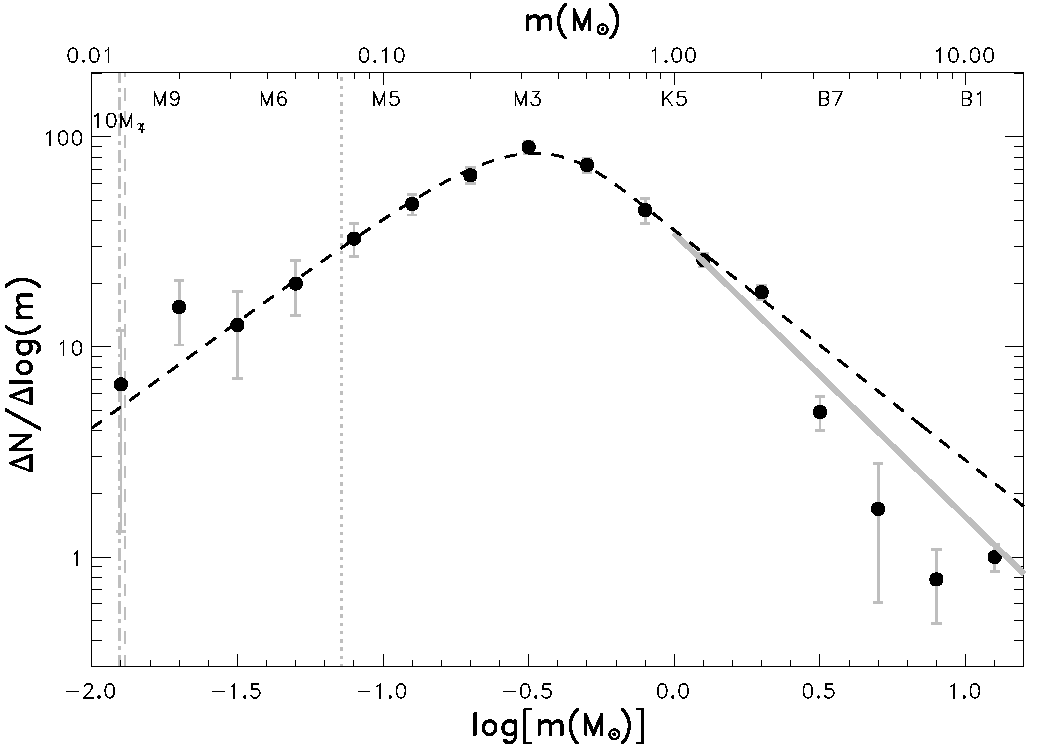
\includegraphics[width=.33\linewidth]{f_9-8.pdf}} &
		\subfloat{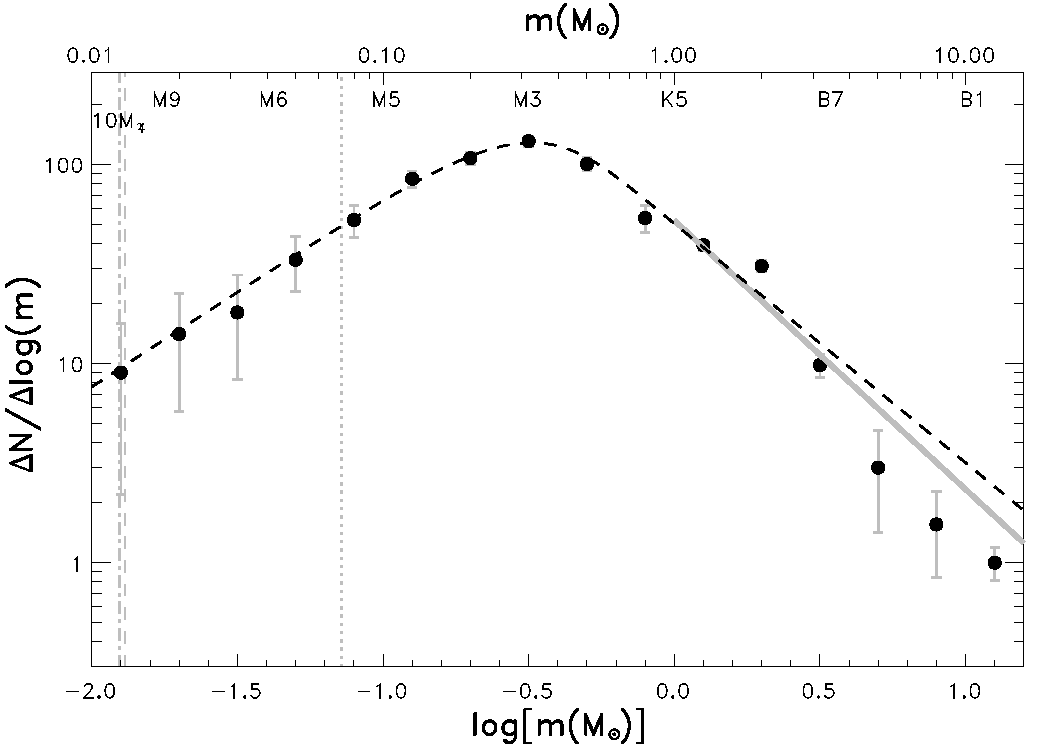
\includegraphics[width=.33\linewidth]{f_9-9.pdf}} 
	\end{tabular}
	\caption[Parameterizations fitted to the 25 Ori system IMFs]{Parameterizations fitted to the 25 Ori system IMFs. Left, central and right panels are the system IMFs considering the areas by \citet[0.5$^\circ$ radius; ][]{Downes2014}, \citet[0.7$^\circ$ radius; ][]{Briceno2018} and \citet[1.0$^\circ$ radius; ][]{Briceno2005,Briceno2007}, respectively. Top, middle and bottom panels show the three-part power-law, lognormal and tapered power-law functions, respectively, fitted to the system IMFs. As a reference, the gray line shows the \citet{Salpeter1955} slope ($\Gamma=1.35$). The rest of the symbols and lines are the same as in Figure \ref{fig_IMF:imf}.
	\label{fig_IMF:imf_par}}
\end{figure*}

\begin{table*}
\caption{Parameterizations fitted to the 25 Ori system IMF.}
  \scriptsize
  \label{tab_IMF:imf}
  \setlength{\tabcolsep}{5pt}
  \begin{threeparttable}
 	\begin{tabular}{@{\extracolsep{2pt}}ccccccccc@{}}
    \toprule
		Area           & \multicolumn{2}{c}{Lognormal} & \multicolumn{3}{c}{Triple Power Law}           & \multicolumn{3}{c}{Tapper Power Law} \\
   \cline{2-3}
   \cline{4-6}
   \cline{7-9}
        radius	    & $m_c$        & $\sigma$       & $\Gamma_1$ ($m\le0.3\ M_\odot$) & $\Gamma_2$ ($0.3<m/M_\odot<1.0$)  & $\Gamma_3$ ($m\ge1.0\ M_\odot$)  & $\Gamma$      & $m_p$         & $\beta$      \\
        ($^\circ$)  & $(M_\odot)$  &                &                               &                &               &               & $(M_\odot)$   &             \\
    \midrule
		0.5$^a$       & 0.30$\pm$0.05 & 0.49$\pm$0.07 & -0.73$\pm$0.08 & 0.88$\pm$0.05 & 1.29$\pm$0.10 & 1.14$\pm$0.23 & 0.32$\pm$0.07 & 2.10$\pm$0.18 \\
		0.7$^b$       & 0.31$\pm$0.04 & 0.46$\pm$0.05 & -0.78$\pm$0.06 & 0.91$\pm$0.11 & 1.48$\pm$0.18 & 1.10$\pm$0.09 & 0.31$\pm$0.03 & 2.11$\pm$0.09 \\
		1.0$^c$       & 0.27$\pm$0.02 & 0.42$\pm$0.03 & -0.84$\pm$0.07 & 0.89$\pm$0.07 & 1.59$\pm$0.18 & 1.20$\pm$0.13 & 0.31$\pm$0.05 & 2.15$\pm$0.18 \\
    \bottomrule
 	\end{tabular}
  \begin{tablenotes}[para,flushleft]
	$^a$By \citet{Downes2014}.\\
	$^b$By \citet{Briceno2005,Briceno2007}.\\
	$^c$By \citet{Briceno2018}.
  \end{tablenotes}
 \end{threeparttable}
\end{table*}

\subsubsubsection{Comparison of the 25 Ori system IMF with Other Studies}
\label{sec_IMF:imf_comparison}
Before comparing the system IMF reported here with that in other regions, we considered the 25 Ori system IMF obtained by \citet{Downes2014}. They found that the system IMF in their entire survey (3x3 deg$^2$ around 25 Ori) is well described by either two power laws with slopes $\Gamma_a=-2.73\pm0.31$ and $\Gamma_b=-0.32\pm0.41$ for the mass ranges $0.02\le m/M_\odot\le0.08$ and $0.08\le m/M_\odot\le0.5$, respectively, or a lognormal function with parameters $m_c=0.21\pm0.02$ and $\sigma=0.36\pm0.03$ for the whole studied mass range. Additionally, for the system IMF of the overdensity (0.5$^\circ$ radius), they obtained $\Gamma_a=-2.97\pm0.02$ and $\Gamma_b=-0.63\pm0.04$, and $m_c=0.22\pm0.02$ and $\sigma=0.42\pm0.05$ in the corresponding mass ranges. Those $m_c$ and $\sigma$ values are slightly lower and the slope for substellar masses is quite steeper than those reported here. We mainly attribute these differences between both system IMFs to differences in the corresponding samples and also in the procedures used in both works. Here, we considered the mass range $0.01<M/M_\odot<13$ against $0.03<M/M_\odot<0.8$ from \citet{Downes2014}, in which some level of incompleteness was expected in the less and more massive system IMF bins. Particularly, we estimated that $\sim$10\% of our member candidates with $I_c$ magnitudes between 17 and 19 are unresolved sources in the CDSO catalog used by \citet{Downes2014}, which could result in that fraction of missed candidates in their selection in this brightness range due to the spatial resolution differences between the DECam and CDSO catalogs, as shown in Table \ref{tab_IMF:catalogs}. Additionally, both system IMF estimations followed different procedures: \citet{Downes2014} interpolates masses simultaneously from $T_{eff}$ and $L_{bol}$ in the H-R diagram while here we obtained the system IMF using the mass-luminosity relationship explained in Section \ref{sec_IMF:mass-luminosity}. Thus, in this work we present the updated version of the system IMF of 25 Ori across the whole mass range, which allow us to rule-out the possible low number of BDs suggested by \citet{Downes2014} when comparing with the Galactic-disk IMF from \citet{Chabrier2003b}.

In order to contribute to the understanding of the origin of the IMF and its relation with the environment, we compared the parameters of the multi-segmented power-law and lognormal functions fitted to the 25 Ori system IMF with those in Table \ref{tab_IMF:imf_literature}, mainly because those IMFs cover a wide mass range as that presented here, and with other studies of interest to include as well the tapered power-law parameterizations. In these comparisons we assumed similar binarity properties for the different clusters and similar spatial resolutions of the surveys.

The best fitted lognormal function to the 25 Ori system IMF are roughly consistent, within the uncertainties, with those obtained in the clusters mentioned in Table \ref{tab_IMF:imf_literature}. The values of $m_c$ range from 0.25 to 0.36, with the most widely varying values in the oldest associations. $\sigma$ takes values between 0.38 and 0.53, considering only those obtained for masses $<$1 $M_\odot$. Also, these values are consistent with a set of young clusters in \citet{Bayo2011}. Though we compared the best fitting lognormal function, we point out that this functional form tends to underestimate the number of BDs in 25 Ori. A similar result was reported in $\sigma$ Ori by \citet{PenaRamirez2012}. 

From the power-law fit, the slope we obtained for intermediate/high-masses is consistent with the \citet{Salpeter1955} slope ($\Gamma=1.35$) and with the most representative slope for $m\ge1\ M_\odot$ from a large sample of stellar associations in \citet{Bastian2010}, which covers a diversity of physical conditions such as age, metallicity and total mass. However, this slope is slightly steeper than those for most clusters in Table \ref{tab_IMF:imf_literature}, nevertheless, it is worth to mentioning the different break masses considered in those studies. In most of the studies in the table, this slope is fitted for masses down to the peak of the IMFs ($\sim0.3\ M_\odot$), while for the case of 25 Ori, it is better described by a dual power-law with a break at 1 $M_\odot$ (see Figure \ref{fig_IMF:imf}). However, if we consider the break at $\sim0.5\ M_\odot$, the slope for masses larger than this value is somewhat shallower than when considering the break at 1 $M_\odot$ and is more consistent with those for the clusters in the table.

The tapered power-law fit to our system IMF is roughly consistent with that fitted to an extended sample of young clusters (25 Ori not included) by \citet{DeMarchi2010} and \citet{Bastian2010}, which has the parameters $\Gamma=1.1\pm0.2$, $m_p=0.23\pm0.10$ and $\beta=2.4\pm0.4$. The $m_p$ value is slightly higher in our system IMF but the differences are in agreement within the errors.

These comparisons indicate that the 25 Ori system IMF is similar to that of a diversity of stellar clusters, which supports the idea that the shape of the IMF is largely insensitive to environmental properties, as predicted by the models from \citet{Bonnell2006} and \citet{Elmegreen2008}.

Also, we emphasize that the 25 Ori system IMF is a smooth function across the whole mass range, in the sense that we do not observe any bimodality behavior as in the ONC \citep{Drass2016}.

\subsubsection{BD/star ratio}
\label{sec_IMF:BD_star_ratio}
An alternative quantity that indicates the relative efficiency to form stellar and substellar objects is, precisely, the ratio between BDs and stars. We worked with the $R_{ss}$ definition by \citet{Briceno2002}, which considers objects with masses between 0.02 and 10 $M_\odot$ and the BD-star limit at 0.08 $M_\odot$. If we consider radius values between 0.4 and 1.1$^\circ$ by steps of $0.1^\circ$, $R_{ss}$ takes values between 0.14 and 0.16, which are basically the same within the uncertainties. For the 25 Ori areas of 1.0, 0.7 and 0.5$^\circ$ radius, $R_{ss}$ is $0.14\pm0.03$, $0.15\pm0.02$, $0.15\pm0.02$, respectively.

The $R_{ss}$ value representative of 25 Ori is $0.15\pm0.03$ i.e. for each 7 stars in 25 Ori we roughly expect 1 BD. This value is consistent with those found in regions with low stellar density as Blanco 1 \citep{Moraux2007a} and with higher stellar densities such as the Trapezium \citep{Muench2002}, ONC \citep{Kroupa-Bouvier2003}, NGC 6611 \citep{Oliveira2009}, Chamaeleon-I and Lupus-3 \citep{Muzic2015}, IC 348 \citep{Scholz2013} and RCW 38 \citep[as a lower quote; ][]{Muzic2017}. Furthermore, the BD to star ratio we found in 25 Ori is consistent with that on the Galactic plane \citep{Bihain-Scholz2016}. The fact that such widely differing regions show a similar ratio of BDs to stars suggests that the environment plays a small role, if any, in the formation of substellar and stellar objects.

%++++++++++++++++++++++++++++++++++++++++++++
\subsubsection{Spatial Distribution}
\label{sec_IMF:spatial_distribution}
Taking advantage of the large spatial coverage of our candidate sample, we examined the system IMF for possible variations with the radius. In Table \ref{tab_IMF:imf} and Figure \ref{fig_IMF:imf_par} we observe that the slope for the intermediate/high-mass stars becomes steeper with the radius, which is also obtained for other radii between 0.4 and 1.1$^\circ$ with steps of 0.1$^\circ$. This behavior is not very pronounce and is largely contained within the uncertainties. Also, we observed that the peak of the system IMF appears to move towards lower masses with the radius, taking values from 0.35 to 0.26 $M_\odot$ for radii between 0.4 and 1.1$^\circ$. A similar behavior was observed in the ONC \citep{Hillenbrand2000} and IC 348 \citep{Muench2002}. Nevertheless, for 25 Ori the $m_c$ changes are smaller than the bin size of the system IMF (0.2 dex). Thus, we do not observe any clear tendency of the distribution of the LMSs and intermediate/high-mass stars.

For the very low-mass stars and BDs, we observed that the slope fits to the system IMF are in agreement, within the uncertainties, for the different 25 Ori radii. This slope also keeps constant for other radii between 0.4 and 1.1$^\circ$, which suggests that the very low-mass stars and BDs do not have any preferential distribution. 

Hence, we do not observe any significant differences between the 25 Ori system IMF for different radii, as suggested by \citet{Downes2014} from the analysis of the spatial distribution of low mass stars and substellar objects.

Additionally, the similar $R_{ss}$ values obtained in previous section are an indicative that the substellar and stellar population have similar spatial distribution across the entire area of 25 Ori.

\subsubsection{Gravitational State of 25 Ori}
\label{sec_IMF:unbound}
As mentioned by \citet{Lada-Lada2003}, most clusters are dissolved before they reach an age of 10 Myr; only less than 10\% reach older ages and about 4\% survive longer than 100 Myr. 25 Ori is just at this critical point and no conclusive results about its gravitational state have been presented \citep{McGehee2006,Downes2014}. Any cluster, to be gravitationally bound, its escape velocity, $v_{esc}=(2GM/R)^{(1/2)}$, must be larger than its velocity dispersion \citep{Sherry2004}.

Directly counting in the mass distributions shown in Figure \ref{fig_IMF:imf}, we obtained a total mass of $168\pm8$, $236\pm10$ and $355\pm14$ $M_\odot$ contained in 25 Ori inside areas of 0.5, 0.7 and 1.0$^\circ$ radius, respectively. The fraction of these masses contained in BDs is $1.34\pm0.35$, $1.34\pm0.32$ and $1.35\pm0.29$\%, respectively. Similar values are obtained for other radius between 0.4 and 1.1$^\circ$, which also indicates, as from the $R_{ss}$ ratio, alike spatial distribution of the substellar and stellar population of 25 Ori.

Considering the total mass of 355 $M_\odot$ inside a radius of 1.0$^\circ$, which corresponds to 6.2 pc at a distance of 356 pc, the resultant $v_{esc}$ is 0.7 km s$^{-1}$. A similar $v_{esc}$ is obtained if considering the total mass inside the 0.7 or 0.5$^\circ$ radius. This $v_{esc}$ is about 3 times smaller than the velocity dispersion of 2 km s$^{-1}$ in 25 Ori \citep{Briceno2007}, which indicates that 25 Ori is an unbound association. We estimated that to be a gravitationally bound cluster, 25 Ori should have about 10 times more mass than that estimated here, which implies an unrealistic number of more than 6000 members, or to have a significantly smaller velocity dispersion.

\subsection{Summary and Conclusions}
\label{sec_IMF:conclusions}
By combining optical and NIR photometry from DECam, CDSO, UCAC4 and $Hipparcos$, and VISTA and 2MASS, respectively, we selected a sample of 1687 photometric member candidates in an area of 1.1$^\circ$ radius in 25 Ori on the basis of their position in color-magnitude and color-color diagrams. This sample covers an $I_c$ range between 5.08 and 23.30 mag, which corresponds to a mass range from $0.011$ to 13.1 $M_\odot$. The completeness of the sample is at 0.012 $M_\odot$, which is just beyond the deuterium burning limit (0.013 $M_\odot$), and also  includes the most massive stars in 25 Ori. We estimated a contamination of 20\% for the LMS candidates, but it increases for the intermediate-mass candidates due to giant and subgiant stars and for BD candidates due to extragalactic sources.

Additionally, we discussed and/or considered, in the context of 25 Ori, the following uncertainties and biases to be taken into account when determining the mass distribution: spatial completeness, photometric sensitivity, IR excesses, chromospheric activity, unresolved binaries and missed members.

With the sample of member candidates we constructed the system IMF of 25 Ori for different areas, which is complete down to 12 $M_{Jup}$ to 13.1 $M_\odot$ and is one of the few system IMFs covering the whole mass range of a stellar cluster \citep[e.g. the $\sigma$ Ori system IMF by ][]{PenaRamirez2012}. This system IMF is a smooth function across the whole mass range. We parameterized the resultant system IMF using a three-part power-law, a lognormal and a tapered power-law function to compare it with other studies. We observed that a lognormal function well-fitted to the peak of the mass distribution underestimates the BD population of 25 Ori.

The system IMF presented here shows a number of BDs larger than reported by \citet{Downes2014}. We found this difference can be mainly explained by issues related to the spatial resolution and completeness of the CDSO as well as differences in the procedures for computation of the system IMF. The updated system IMF presented in this work allow us to ruled-out the possible low number of BDs suggested by \citet{Downes2014}.

The 25 Ori system IMF does not present significant differences in comparison with other clusters having different physical properties, which suggests that the conversion of gas into stars and BDs has minimum influence by the environmental properties, as predicted by some models \citep[e.g. ][]{Bonnell2006,Elmegreen2008}.

We estimated the substellar to stellar ratio of 25 Ori, which has a representative value of $0.15\pm0.03$. This ratio is consistent with those in other regions with different stellar densities which is an indicative that the formation of BDs and stars occurs in a similar way in different environments.

There are no significant variations of the 25 Ori system IMF with the radius and the BD/star ratio is similar for different radii. These results indicate that the substellar and stellar objects do not have any preferential distribution.

Comparing the escape velocity estimated for 25 Ori and its velocity dispersion, we found that 25 Ori is an unbound association. In fact, 25 Ori should have about 10 times more mass or a significantly smaller velocity dispersion to be considered as a gravitationally bound cluster.

The system IMF of 25 Ori we present in this work was constructed with photometric member candidates. To determine the membership of each candidate it is necessary a follow up spectroscopy. Thus, we could determine the distribution of the masses of the confirmed members. This kind of study requires the use of several multi-fiber spectrographs to have full coverage of the brightness range and spatial distribution. In this direction, we have an ongoing spectroscopic survey about 85\% complete, which will be part of a future work. 

%% APPENDICES
%\subsection[Appendix: DECam Photometry Calibration]{Appendix: Calibration of the DECam Photometry}
%\label{sec_app_IMF:DECam_calibration}
%To calibrate our DECam photometry we first added the zero point of 25.18 mag from the image headers to the instrumental magnitudes. Then, we compared these instrumental magnitudes with the $i$ magnitudes in the DECam system obtained using the $i$ and $z$-band photometry from SDSS according to Transformation \ref{eq_IMF:DECam_instrumental}\footnote{\url{http://www.ctio.noao.edu/noao/content/Photometric-Standard-Stars-0\#transformations}}.
%
%\begin{equation} \label{eq_IMF:DECam_instrumental}
%	i_{DECam}    = i + 0.014 - 0.214*(i-z) - 0.096*(i-z)^2
%\end{equation}
%
%where $i_{DECam}$ are in the DECam system and $i$ and $z$ magnitudes are in the SDSS system.
%
%The comparison was done for sources having colors $i-z<0.8$ mag (valid range of the transformation), considering sources not having a high probability of being variable stars according to the CIDA Variability Survey of Orion \citep[][]{Briceno2005,Mateu2012,Briceno2018} and for sources having $i$ and $z$-band photometric errors lesser than 0.05 mag. The mean value of the resultant residuals is 0.637 mag. Thus, we added this value to our DECam photometry to calibrate it. In Figure \ref{fig_IMF:DECam_instrumental} we show the residual between our calibrated photometry and that in the DECam system using the SDSS catalog. The typical residuals are -0.001 mag with a RMS of 0.038 mag.
%
%\begin{figure}[ht!]
%	\begin{minipage}{0.60\textwidth}
%		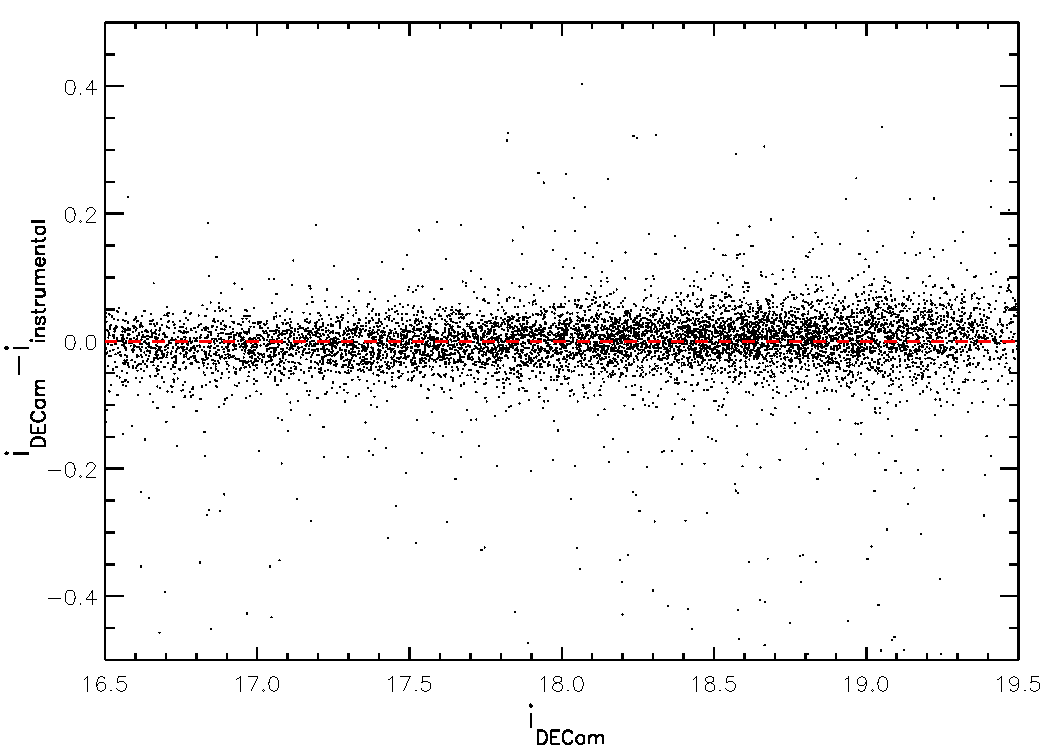
\includegraphics[width=1.00\textwidth]{f_A1.pdf}
%	\end{minipage} \hfill
%	\begin{minipage}{0.35\textwidth}
%		\caption[Calibration of the DECam photometry.]{Residual between our calibrated photometry from DECam and the $i$-band photometry in the DECam system obtained using the SDSS catalog.}
%		\label{fig_IMF:DECam_instrumental}
%	\end{minipage}
%\end{figure}
%
%\subsection[Appendix: Photometry Transformation]{Appendix: Transformation of the UCAC4 and DECam Photometry to $I_c$ Magnitudes}
%\label{sec_app_IMF:photometry_transformation}
%We used transformations from \citet{Jordi2006} and empirical relations obtained directly from our data to convert the $i$-band magnitudes from the UCAC4 and DECam catalogs to the $I_c$-band magnitudes.
%
%\subsubsection{UCAC4 Data}
%As the transformations from \citet{Jordi2006} relate the SDSS and Cousins photometric systems, we first checked that the UCAC4 photometry are in the SDSS system.
%
%The $r$ and $i$-band photometry in UCAC4 came from the AAVSO \footnote{\url{https://www.aavso.org}} Photometric All-Sky Survey \citep[][]{Henden2016}. These data were taken using the $r'$ and $i'$-band filters from SDSS, whose magnitudes are on the AB system and are close to the $r$ and $i$ magnitudes of SDSS\footnote{\url{http://www.sdss3.org/dr8/algorithms/fluxcal.php\#SDSStoAB}}. In Figure \ref{fig_IMF:SDSS_UCAC4} we show the residuals between the $r$ and $i$ magnitudes from SDSS and UCAC4 as a function of the SDSS magnitudes. We did not consider the sources having $>90\%$ probability of being variables according to the CVSO and only worked with sources having photometric errors lesser than 0.05 mag. In average, these residuals are basically zero for sources brighter than the SDSS saturation limit ($\sim$14 mag), which indicates that the $r$ and $i$-band photometries from UCAC4 can be consider to be in the SDSS photometric system.
%
%\begin{figure*}[ht!]
%	\centering
%	\begin{tabular}{cc}
%		\subfloat{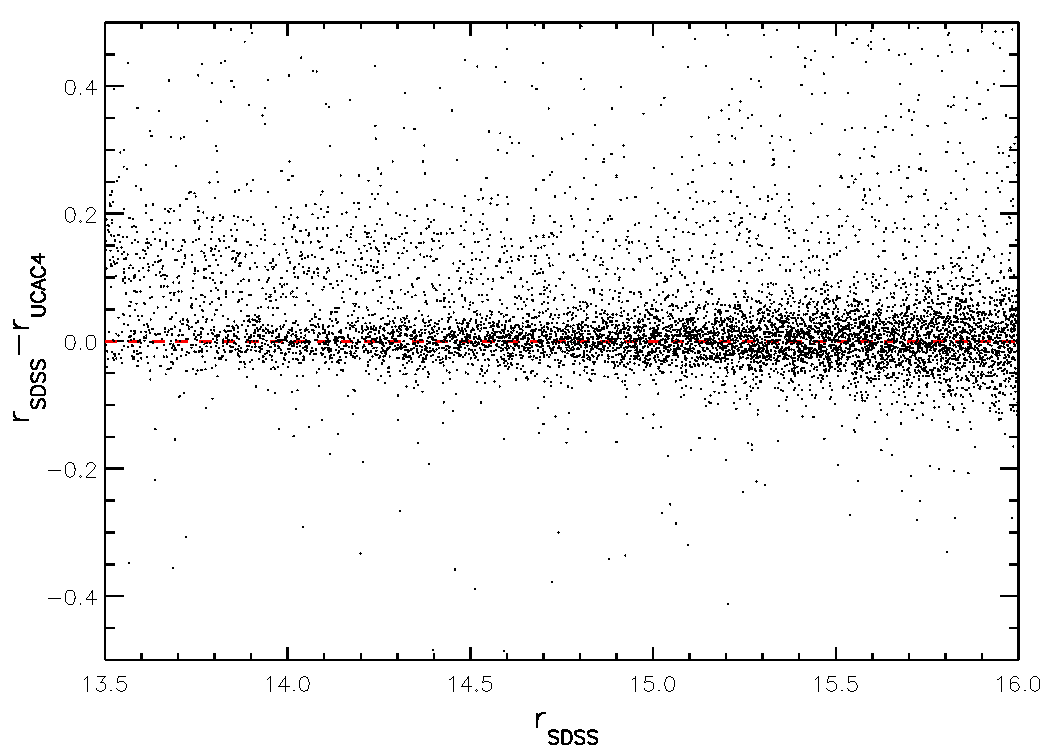
\includegraphics[width=.50\linewidth]{f_B1-1.pdf}} & 
%		\subfloat{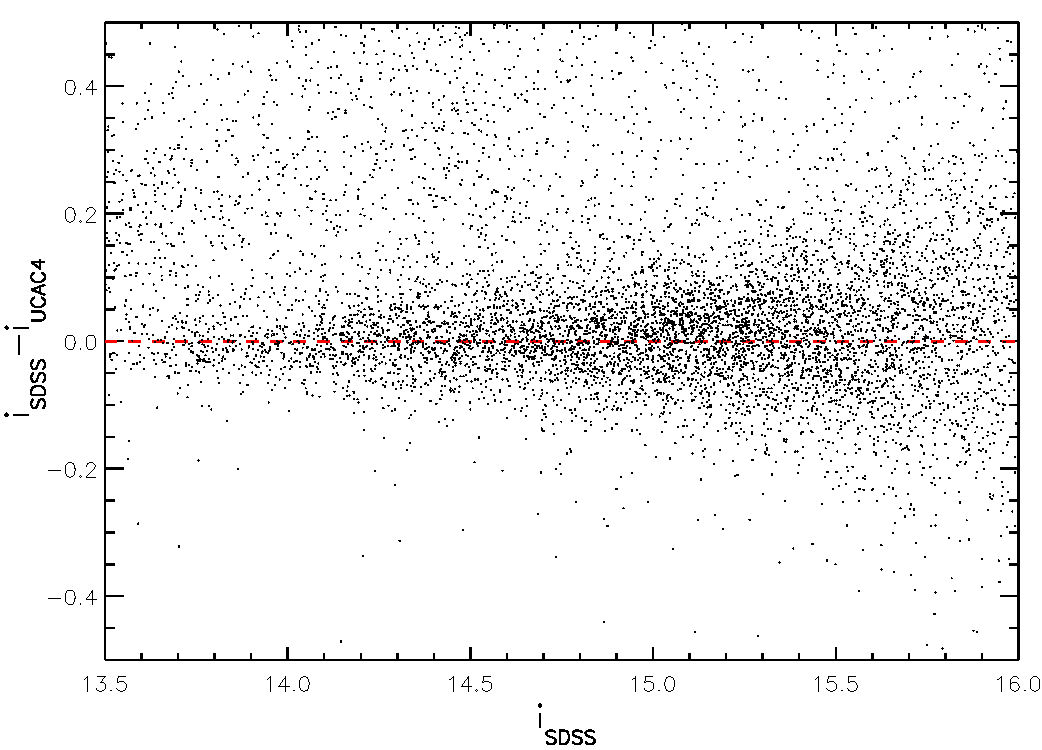
\includegraphics[width=.50\linewidth]{f_B1-2.pdf}} 
%	\end{tabular}
%	\caption[UCAC4 photometry in the SDSS system.]{Residual between the SDSS and UCAC4 photometries as a function of the SDSS magnitudes in the $r$ and $i$-bands (left and right panels, respectively).}
%	\label{fig_IMF:SDSS_UCAC4}
%\end{figure*}
%
%Thus, we worked with the following transformations from \citet{Jordi2006}, which use the $r$ and $i$-band magnitudes from SDSS:
%
%\begin{equation} \label{eq_IMF:UCAC_1}
%	R_c-r = -0.153*(r-i) - 0.117
%\end{equation}
%\begin{equation} \label{eq_IMF:UCAC_2}
%	R_c-I_c = 0.930*(r-i) + 0.259
%\end{equation}
%
%Subtracting Transformation \ref{eq_IMF:UCAC_2} from Transformation \ref{eq_IMF:UCAC_1}:
%
%\begin{equation} \label{eq_IMF:UCAC_3}
%	I_c-r = -1.083*(r-i) -0.376
%\end{equation}
%
%We used Transformation \ref{eq_IMF:UCAC_3} to obtain the $I_c$ magnitudes considering the $r$ and $i$-band photometry from UCAC4. We compared the resultant $I_c$ magnitudes with those from the CDSO, which are already in the Cousin system. In the left panel of Figure \ref{fig_IMF:trasformation_UCAC4} we show the residual between the $I_c$ magnitudes from the CDSO and UCAC4, where we can see that the peak of the residual distribution is somewhat deviated from zero. Therefore, we did slight modifications to the coefficients of Transformation \ref{eq_IMF:UCAC_3} to have average residuals closer to zero. The resulting transformation is:
%
%\begin{equation} \label{eq_IMF:UCAC_4}
%	I_c-r = -1.323*(r-i) -0.353
%\end{equation}
%
%In the right panel of Figure \ref{fig_IMF:trasformation_UCAC4} we show the $I_c$ residuals between the CDSO and UCAC4 photometries after applying Transformation \ref{eq_IMF:UCAC_4} to the UCAC4 data. The peak of the $I_c$ residual histograms are essentially zero, with a RMS of 0.07 mag for all the sources within the CDSO saturation limit and the UCAC4 completeness limit (13-14.75 mag).
%
%\begin{figure*}[ht!]
%	\centering
%	\begin{tabular}{cc}
%		\subfloat{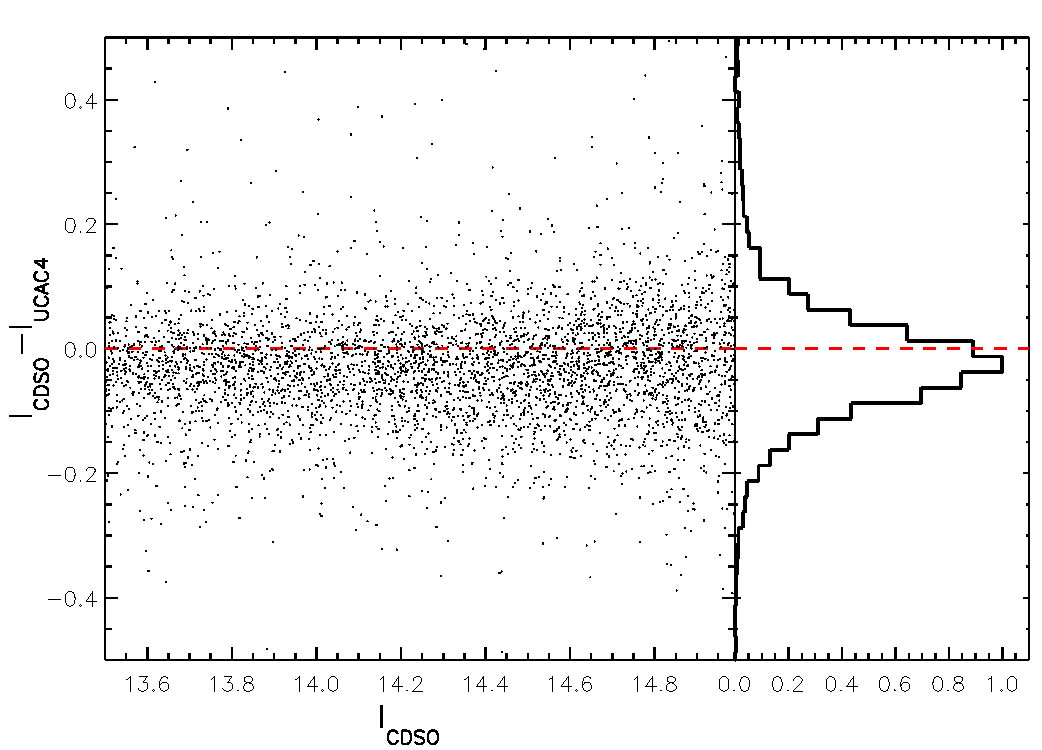
\includegraphics[width=.50\linewidth]{f_B2-1.pdf}} & 
%		\subfloat{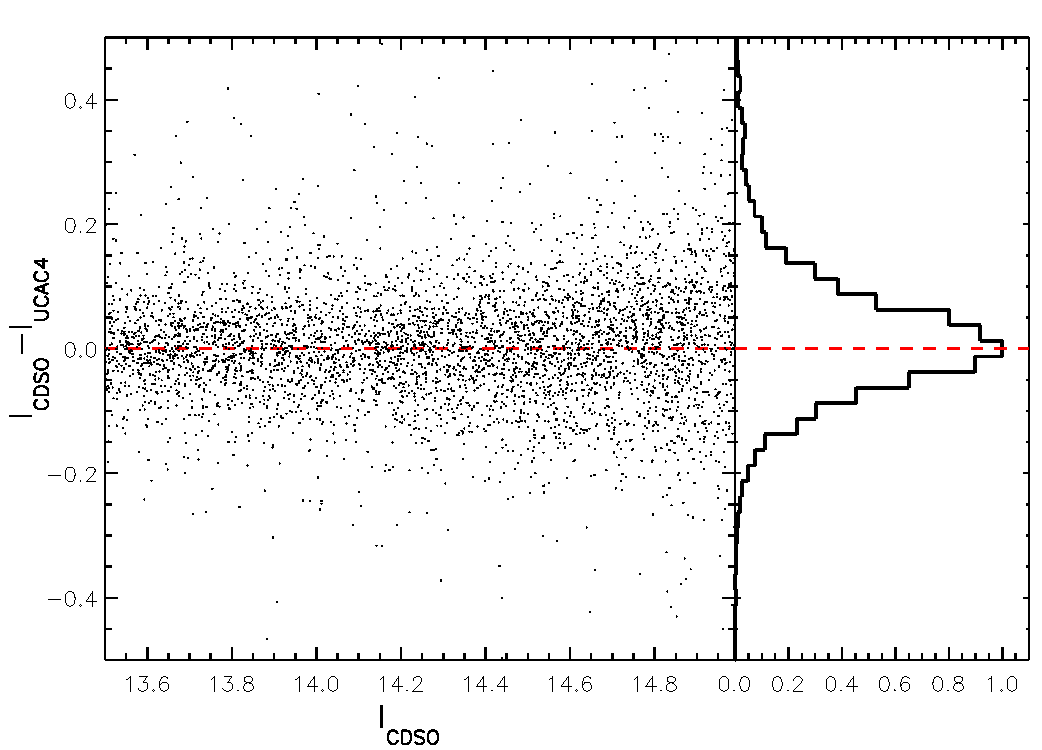
\includegraphics[width=.50\linewidth]{f_B2-2.pdf}} 
%	\end{tabular}
%	\caption[Transformation of the UCAC4 photometry to the Cousins system.]{$I_c$-residuals between the CDSO and UCAC4 after applying Transformation \ref{eq_IMF:UCAC_3} \citep[left panel; ][]{Jordi2006} and Transformation \ref{eq_IMF:UCAC_4} (right panel), which is a slight modification of Transformation \ref{eq_IMF:UCAC_3}.}
%	\label{fig_IMF:trasformation_UCAC4}
%\end{figure*}
%
%\subsubsection{DECam Data}
%The $i$ filter used in our DECam observations is similar to the $i$ filter from SDSS (NOAO Data Handbook\footnote{\url{http://ast.noao.edu/sites/default/files/NOAO\_DHB\_v2.2.pdf}}). However, there is a color dependence to transform the DECam data to the SDSS system. As we only have DECam photometry taken with the $i$ filter, in addition to these data we worked with the $Z$-band photometry from VISTA. This way, we will transform the DECam photometry only for the sources with VISTA counterpart, which is not an issue because for the selection of member candidates we used both catalogs. The $Z$-band photometry from VISTA is in the Vega system and to convert it to $z'$-band magnitudes in the AB system it is necessary to add the zero-point of 0.58 mag \citep{Pickles2010}. These $z'$-band magnitudes are not exactly the same as the $z$-band magnitudes in the SDSS system, there is a small shift of 0.02 mag which should be subtracted\footnote{\url{http://www.sdss3.org/dr8/algorithms/fluxcal.php\#SDSStoAB}}. Therefore, we added 0.56 mag to the $Z$-band photometry from VISTA to obtain the $z$-band magnitudes in the SDSS system. In Figure \ref{fig_IMF:trasformation_VISTA} we show the residuals between the $z$ magnitudes directly from SDSS and from VISTA after the addition of the offset. We removed the sources with $>90\%$ probability of being variable according to the CVSO catalog and we only considered sources with errors lesser than 0.05 mag. The average of the resultant residuals is -0.008 mag with a RMS of 0.04 mag.
%
%\begin{figure}[ht!]
%	\begin{minipage}{0.60\textwidth}
%		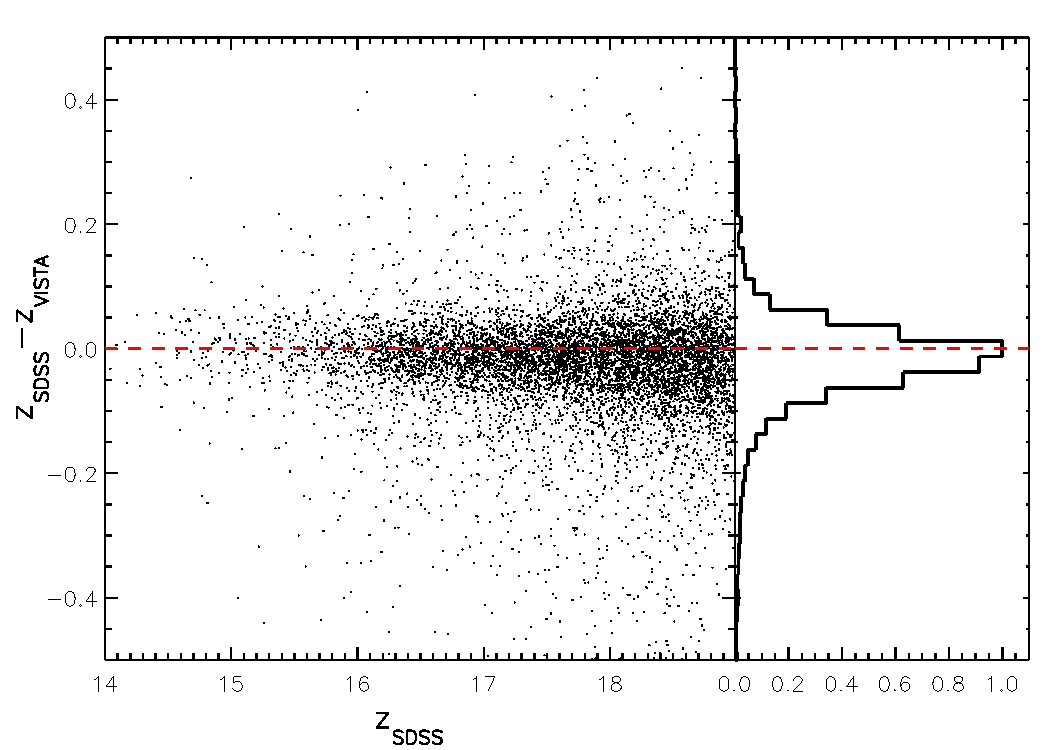
\includegraphics[width=1.00\textwidth]{f_B3.pdf}
%	\end{minipage} \hfill
%	\begin{minipage}{0.35\textwidth}
%		\caption[$Z$ magnidutes from VISTA in the SDSS system.]{Residuals between the $z$ magnitudes in the SDSS system directly from the SDSS catalog and from VISTA.}
%		\label{fig_IMF:trasformation_VISTA}
%	\end{minipage}
%\end{figure}
%
%In left panel of Figure \ref{fig_IMF:trasformation_DECam_SDSS} we show the color dependence of the residuals between our calibrated DECam data and those from SDSS as a function of the $i-z$ color combining the calibrated photometry from DECam and the photometry from VISTA converted to the SDSS system. The second order function that best fits the residuals is:
%
%\begin{equation} \label{eq_IMF:DECam_SDSS}
%	i-i_{DECam} = -0.008+ 0.194*(i_{DECam}-z)+ 0.381*(i_{DECam}-z)^2
%\end{equation}
%
%where $i_{DECam}$ are in the DECam system and $i$ and $z$ in the SDSS system.
%
%We used Transformation \ref{eq_IMF:DECam_SDSS} to convert our calibrated DECam photometry to the SDSS system. In right panel of Figure \ref{fig_IMF:trasformation_DECam_SDSS} we show the residuals between the $i$-band magnitudes in the SDSS system obtained directly from SDSS and from our calibrated DECam data. The average of the residuals is 0.002 mag with a RMS of 0.04 mag.
%
%\begin{figure*}[ht!]
%	\centering
%	\begin{tabular}{cc}
%		\subfloat{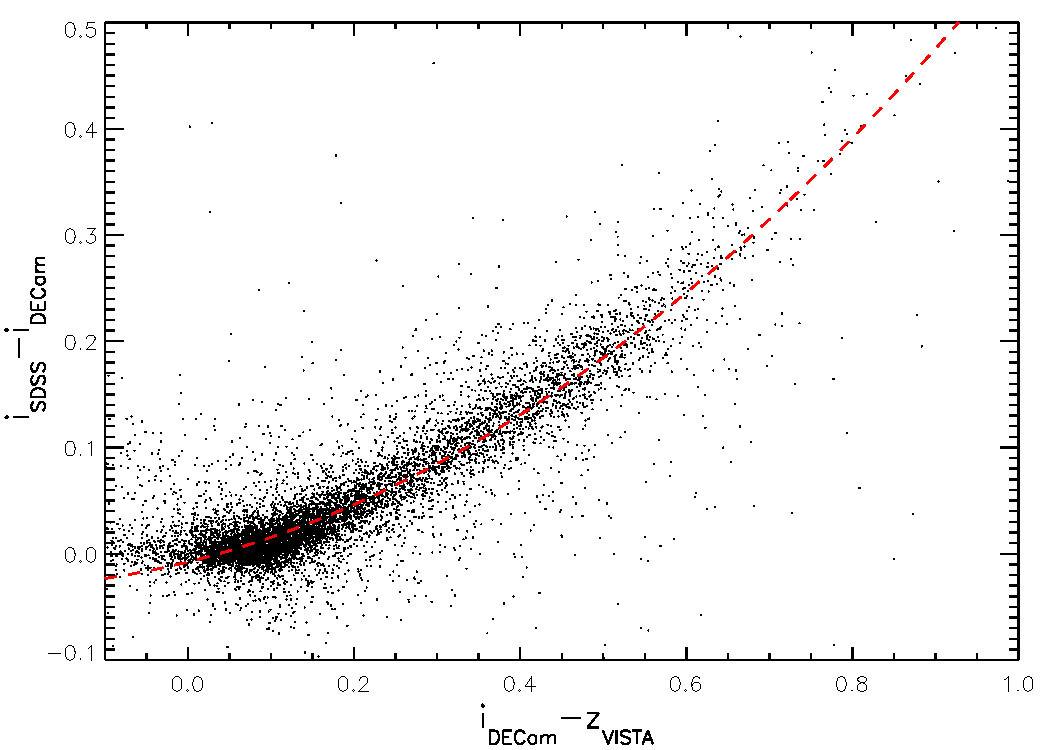
\includegraphics[width=.50\linewidth]{f_B4-1.pdf}} & 
%		\subfloat{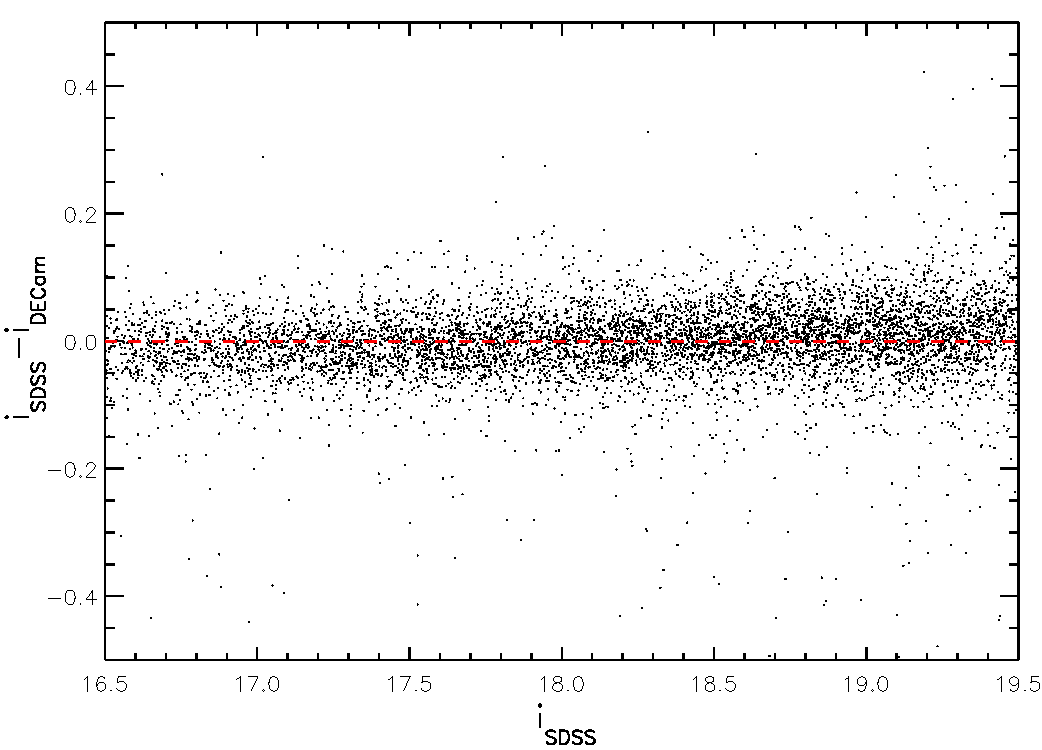
\includegraphics[width=.50\linewidth]{f_B4-2.pdf}} 
%	\end{tabular}
%	\caption[Transformation of the DECam photometry to the SDSS system.]{{\bf Left panel:} Residuals between the $i$ magnitudes from the SDSS catalog and from our calibrated DECam data as a function of the $i-z$ color from DECam and VISTA data in the SDSS system. The red dashed line indicate the second order function fitted to the residuals. {\bf Right panel:} Residuals between the $i$-band photometries in the SDSS system directly from SDSS and from DECam after applying Transformation \ref{eq_IMF:DECam_SDSS}.}
%	\label{fig_IMF:trasformation_DECam_SDSS}
%\end{figure*}
%
%Finally, once we have both the $i$-band photometry from DECam and the $Z$-band photometry from VISTA in the SDSS system, we converted them to $I_c$ magnitudes in the Cousins system. In left panel of Figure \ref{fig_IMF:trasformation_DECam_CDSO} we show the $i-z$ dependence of the residual between the $I_c$ magnitudes from the CDSO survey and our DECam data in the SDSS system. The second order function fitted to the residual is:
%
%\begin{equation} \label{eq_IMF:DECam_CDSO}
%	I_c-i = -0.406-0.446*(i-z)-0.154*(i-z)^2
%\end{equation}
%
%where $I_c$ is in the Cousins system and $i$ and $z$ the SDSS system.
%
%We used Transformation \ref{eq_IMF:DECam_CDSO} to obtained the $I_c$ magnitudes from our DECam and VISTA photometries in the SDSS system. In right panel of Figure \ref{fig_IMF:trasformation_DECam_CDSO} we show the residuals between the $I_c$ magnitudes from the CDSO and those obtained from our DECam data. We did not consider neither the sources having $>90\%$ probability of being variable stars in the CVSO catalog nor the sources with errors larger than 0.05 mag. The resultant residuals have an average of -0.001 mag with a RMS of 0.04 mag.
%
%\begin{figure*}[ht!]
%	\centering
%	\begin{tabular}{cc}
%		\subfloat{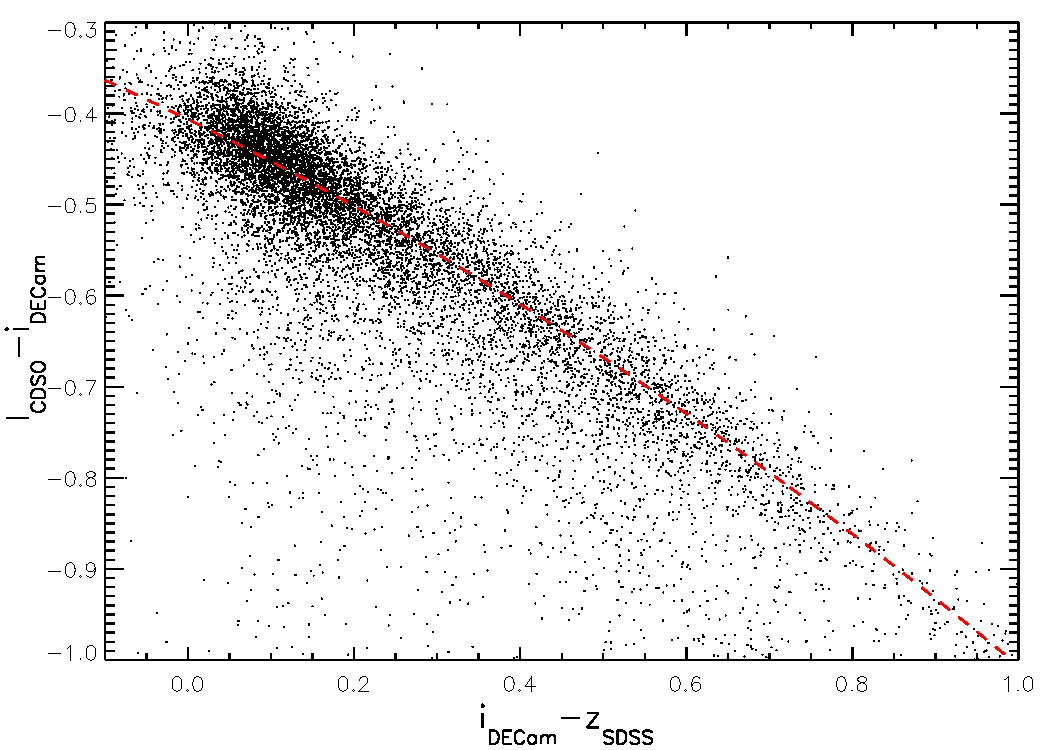
\includegraphics[width=.50\linewidth]{f_B5-1.pdf}} & 
%		\subfloat{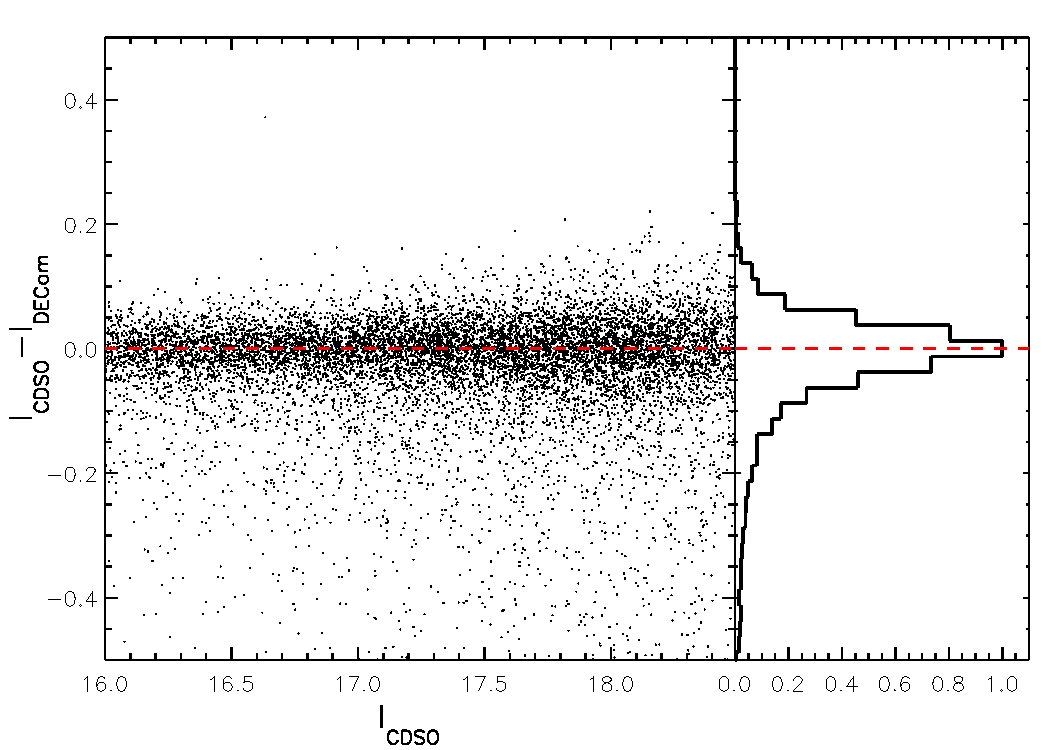
\includegraphics[width=.50\linewidth]{f_B5-2.pdf}} 
%	\end{tabular}
%	\caption[Transformation of the DECam photometry to the Cousins system.]{{\bf Left panel:} Residuals between the $I_c$ magnitudes from the CDSO and the $i$ magnitudes from DECam as a function of the $i-z$ color from DECam and VISTA data in the SDSS system. {\bf Right panel: } Residuals between the $I_c$-band photometries from the CDSO and DECam after applying Transformation \ref{eq_IMF:DECam_CDSO}.}
%	\label{fig_IMF:trasformation_DECam_CDSO}
%\end{figure*}
%
%\subsection{Appendix: 25 Ori Distance}
%\label{sec_app_IMF:distance}
%To estimate the 25 Ori distance, we first compiled a list of 334 unique spectroscopically confirmed members of 25 Ori by \citet{Briceno2005,Briceno2007,Downes2014,Downes2015,Suarez2017,Briceno2018}. Then, we cross-matched this list with the BJ18 catalog to obtain the distances of the confirmed members. This catalog has the point distance estimate and a measure of the uncertainty for each source with Gaia DR2 parallax, even if it is negative and/or has very low signal-to-noise ratio. The uncertainties are represented by upper and lower limits which contain about 68\% (one standard deviation) of the confidence interval. We considered as the uncertainty for each point distance a half of the interval between its upper and lower limits. 90\% of the confirmed members of 25 Ori have distances from BJ18 with uncertainties less than 20\%. In the left panel of Figure \ref{fig_IMF:cum_dist} we show the cumulative distribution of these distances, which cover a range from 127 to 545 pc, but there is a clear concentration of members around the 25 Ori expected distance with 94\% of the member between 250 and 450 pc. From these distances we obtained that 25 Ori is 356$\pm$47 pc away, which is consistent with previous studies \citep{Briceno2007,Downes2014,Suarez2017,Briceno2018,Kounkel2018}.
%
%\subsection{Appendix: 25 Ori Extinction}
%\label{sec_app_IMF:extinction}
%About 96\% of the 334 confirmed members of 25 Ori by \citet{Briceno2005,Briceno2007,Downes2014,Downes2015,Suarez2017,Briceno2018} have reported visual extinctions obtained through spectroscopic analysis. In the right panel of Figure \ref{fig_IMF:cum_dist} we show the cumulative distribution of these extinctions, which go up to 1.88 mag (excluding two members with values of 3.53 and 6.29 mag) but more than 93\% of the members with reported extinction have values lower than 1 mag. Considering values up to 1.88 mag, the mean extinction of the 25 Ori is 0.35$\pm$0.35 mag. If we consider values lower than 1 mag, the 25 Ori mean extinction is 0.29$\pm$0.26 mag. As expected, both values are consistent with previous studies \citep{Kharchenko2005,Briceno2005,Briceno2007,Downes2014,Suarez2017,Briceno2018}. 
%
%\begin{figure*}[ht!]
%	\centering
%	\begin{tabular}{cc}
%		\subfloat{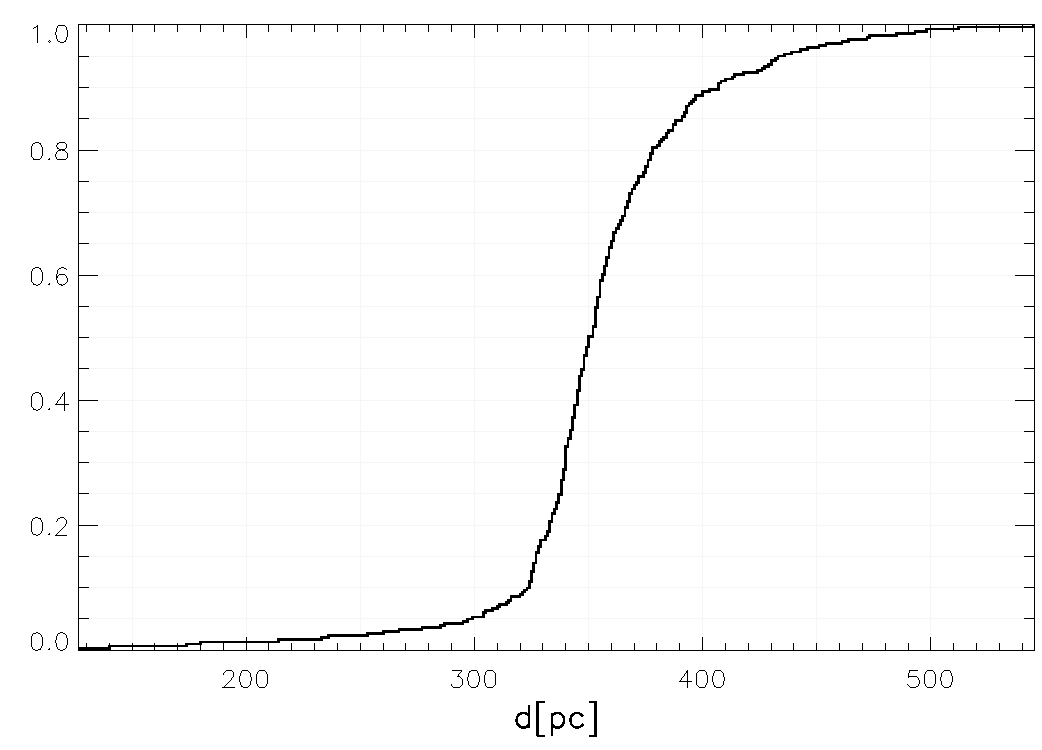
\includegraphics[width=.50\linewidth]{f_D1-1.pdf}} & 
%		\subfloat{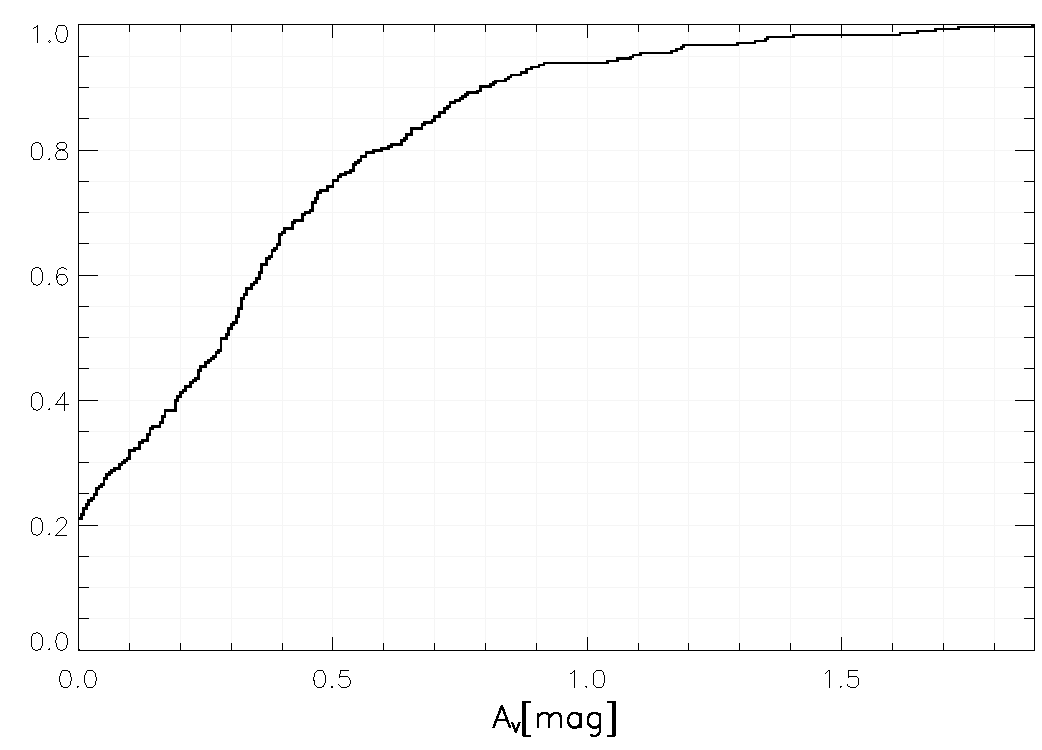
\includegraphics[width=.50\linewidth]{f_D1-2.pdf}} 
%	\end{tabular}
%	\caption[Normalized cumulative distributions of the distances and extinctions of 25 Ori members.]{Normalized cumulative distributions of the distances (left panel) and extinctions (right panel) for the spectroscopically confirmed members of 25 Ori by \citet[][]{Briceno2005,Briceno2007,Downes2014,Downes2015,Suarez2017,Briceno2018}. The distances are from BJ18 and have uncertainties less than 20\%. The extinctions were mostly estimated through spectral analysis and combining optical and NIR photometry.}
%	\label{fig_IMF:cum_dist}
%\end{figure*}
%
%\subsection[Appendix: Distance and Extinction Assignments]{Appendix: Distances and Extinctions for the Member Candidates and Contaminants}
%\label{sec_app_IMF:distance_extinction}
%As we do not have distances and extinctions for all the member candidates (86\% have distances and 18\% have extinctions) and contaminants, we need to assign these values to the whole samples to have consistency with the 25 Ori members. The most common way to do this in photometric studies in the literature is to consider the mean distance and extinction of the cluster for all the member candidates. Here, we can take advantage of the Gaia DR2 parallaxes as well as of the previous spectroscopic studies in 25 Ori to use a statistically more robust technique. Considering the inversion of the normalized cumulative distribution of the BJ18 distances of the 25 Ori confirmed members (left panel of Figure \ref{fig_IMF:cum_dist}), we created random realizations to assign distance values to all our member candidates and contaminants. We also assigned extinction values to these samples in a similar way, but considering the normalized cumulative distribution of the reported extinctions of the 25 Ori confirmed members (right panel of Figure \ref{fig_IMF:cum_dist}). This way, the distance and extinction values we assigned to each candidate and contaminant are consistent with those for the confirmed members of 25 Ori.

%%%%%%%%%%%%%%%%%%%%%%%%%%%%%%%%%%%%%%%%%
\newpage
\section{Spectroscopic Follow-Up}
\label{sec:spectroscopy}

\subsection{Research Statement}
\label{sec:rs_spectroscopy}
The analysis in the previous section was carried out using photometric member candidates and dealing with the contamination present in the sample using statistical techniques. In order to truly determine the membership of each individual source, it is necessary to make a spectroscopic follow-up, which also allows a precise determination of physical parameters such as $T_{eff}$, $A_V$, surface gravity (log $g$), mass and age. This is essential to study various astrophysical phenomena as mass distribution, age spread, evolution of circumstellar disks and the history of star formation. However, such a follow-up spectroscopy is an arduous observational task that implies the uses of several world-wide facilities.
%and when low-mass stars form respect to the most massive members in the cluster evolution history. 

We have an ongoing spectroscopic survey to observed each 25 Ori member candidate in our sample, which consists of 1687 sources with masses from 12 $M_{Jup}$ to 13 $M_\odot$ distributed in an area of 1.1$^\circ$ radius in 25 Ori. In the following sections we describe our spectroscopic observations and summarize the current state of the survey.

%++++++++++++++++++++++++++++
\subsection{OAN-SPM/MES for Intermediate/High-mass Stars}
\label{sec:MES}

\subsubsection{MES Spectra}
\label{sec_echelle:spectra}
To observe the brightest 25 Ori candidates we used the Manchester Echelle Spectrograph \citep[\ac{MES}; ][]{Meaburn1984,Meaburn2003} attached to the 2.1m telescope of the Observatorio Astron\'omico Nacional at San Pedro M\'artir (\ac{OAN-SPM}) in Baja California, Mexico, which allows the acquisition of optical medium-high resolution spectra (\ac{R}=18000 at 5000 \AA). We obtained 24 nights of observing time distributed as follow: 6 nights on December 11-16, 2014 (PI: J. J. Downes), 6 nights on January 06-11, 2015 (PI: J. J. Downes), 6 nights on October 24-29, 2015 (PI: G. Su\'arez) and 6 nights on January 22-27, 2016 (PI: G. Su\'arez). In Table \ref{tab:MES_log} we show the log of our MES observations.
%MES is a single slit spectrograph that uses interference filter to isolote the spectral orders of interest. 

\subsubsubsection{Target Selection}
\label{sec_echelle:targets}
The selection of the MES targets was done on the basis of their positions in the $V$ vs $V-J$ and $H$ vs $H-K$ diagrams using the UCAC4 and 2MASS catalogs. We defined the empirical isochrone traced by the spectroscopically confirmed members by \citet{Briceno2005,Briceno2007,Downes2014} as well as the highly probable members by \citet{Kharchenko2005}. Then, we defined the PMS locus as the region around the empirical isochrone that contains most of the confirmed and highly probable members, and selected the sources lying inside both loci. Additionally, we removed from the candidate selection the sources having low photometric and kinematics probability of being members according to \citet{Kharchenko2005}. The final sample contains 80 member candidates covering an area of 3x3 deg$^2$ around 25 Ori and with $V$-band magnitudes from 4.9 to 12.1, which corresponds to the mass range from 1.6 to 13.1 M$_\odot$ considering the PARSEC-COLIBRI 7 Myr isochrone.

\subsubsubsection{Data Reduction}
\label{sec_echelle:reduction}
During our MES observations we obtained spectra for 77 of these member candidates (96\% of the sample), including all those lying inside the 1.0$^\circ$ radius area of 25 Ori. Additionally, we obtained images for the calibration of the data (bias, flats, ThAr lamps and radial velocity standards). In order to reduce the spectra we used standard \texttt{IRAF}\footnote{IRAF is distributed by the National Optical Astronomy Observatory, which is operated by the Association of Universities for Research in Astronomy (AURA) under a cooperative agreement with the National Science Foundation.} tasks to remove bias, flats and cosmic rays, and to extract the spectra, calibrate in wavelength and normalize the continuum. The final wavelength covered by the 32 Echelle orders (from 32 to 63) in each spectra ranges from 3600 to 7100 \AA\ with a typical resolution of $R=21000$ at H$_\alpha$. In Figure \ref{fig_MES:spectrum} we show an example of a MES spectrum, focusing on some orders of interest.

\subsubsection{Membership Assignment}
\label{sec_MES:membership}
In order to determine the RVs of the MES spectra we used the $fxcor$ task of \texttt{IRAF}, which correlates the spectra with unknown radial velocity with a template spectrum with known radial velocity. For this correlation we considered the following absorption lines: H$_\alpha$ (in order 34), NaI$\lambda\lambda$5890, 5896 (in order 38), MgI$\lambda\lambda\lambda$5167, 5172, 5184 (in order 43), H$_\beta$ (in order 46), CaII$\lambda$3968 (in order 56) and CaII$\lambda$3934 (in order 57). So far, we have obtained radial velocities for 22 targets of the sample (about 30\%) which have values between 10 and 40 km s$^{-1}$ (plus two targets with values of -10 and 50 km s$^{-1}$) and with typical uncertainties of 3 km s$^{-1}$. 

In order to determine which of these targets are members of 25 Ori, we applied several criteria on the basis of their radial velocities, distances and spatial distribution as follows:

$i)$ First, we cross matched our list of targets with Gaia DR2; 99\% of all the MES targets have reliable parallaxes (errors lesser than 20\%). To filter the sample according to their distances, we considered the 25 Ori distance of $356\pm47$ pc (Su\'arez et al. 2018, submitted) and selected the targets located around 25 Ori with a dispersion of $3\sigma$. About 86\% of the MES targets satisfies this criterion. 

$ii)$ Additionally, we selected the targets with radial velocities between 10 and 40 km s$^{-1}$ to have consistency with 25 Ori \citep{Briceno2007}. From the 22 targets for which we have obtained radial velocities from the MES spectra, 14 sources satisfy the distance and radial velocity criteria. Because these sample of 22 targets is representative of the whole sample, we expect that more than 60\% of our targets satisfy these criteria.

$iii)$ Finally, we selected the sources lying inside the 25 Ori estimated area of 1.0$^\circ$ radius. From the 14 targets with distance and radial velocity consistent with 25 Ori, 10 of them are located inside the 25 Ori limits.

In summary, from the 22 targets with radial velocity from the MES spectra and with distances from Gaia DR2, 10 of them have spatial distribution, distances and radial velocities consistent with 25 Ori. Therefore, from the entire sample of MES spectra (77 targets) we roughly expect 35 intermediate/high-mass members of 25 Ori, which is consistent with the expected sources from the 25 Ori system IMF (Su\'arez et al. 2018, submitted).

\begin{table}[ht!] \tiny
\begin{center}
 \caption[OAN-SPM/MES observing log]{OAN-SPM/MES observing log.}
 \label{tab:MES_log}
 \begin{threeparttable}
  	\setlength{\tabcolsep}{11pt}
	\begin{tabular}{lccccccl}
	\toprule
	{\bf Target} & {\bf RA}    & {\bf DEC}    & {\bf UT Date}        & {\bf Airmass} & {\bf T$_{exp}$} & $V$     &  {\bf Comments} \\
	             & (hh:mm:ss)  & (hh:mm:ss)   &(yyyy-mm-ddThh:mm:ss) &               & (s)             & (mag)   &                 \\
	\midrule
	\multicolumn{8}{c}{{\bf 2014B Runs}} \\
	25Ori\_40     & 05:23:14.54 & +02:01:06.9 & 2014-12-11T05:20:32  & 1.415         & 3000             & 11.627 & tiny clouds              \\
	25Ori\_65     & 05:23:45.91 & +01:50:33.4 & 2014-12-11T06:43:46  & 1.189         & 2000             & 9.923  & ---                      \\
	25Ori\_93     & 05:24:16.19 & +01:38:35.7 & 2014-12-11T08:31:15  & 1.168         & 3000             & 11.442 & bad sky                  \\
	25Ori\_86     & 05:24:12.73 & +01:34:12.1 & 2014-12-11T10:35:36  & 1.541         & 3000             & 10.645 & ---                      \\
	25Ori\_105    & 05:24:20.74 & +01:35:26.6 & 2014-12-12T05:27:09  & 1.382         & 6000             & 9.793  & ---                      \\
	25Ori\_128    & 05:24:44.83 & +01:50:47.2 & 2014-12-12T07:27:03  & 1.148         & 2000             & 4.878  & a second spectrum 		\\
	25Ori\_256    & 05:26:11.98 & +01:53:35.7 & 2014-12-12T09:13:14  & 1.233         & 3000             & 9.33   & ---                      \\
	25Ori\_157    & 05:25:11.65 & +01:33:29.7 & 2014-12-12T10:37:16  & 1.571         & 3000             & 9.959  & ---                      \\
	25Ori\_134    & 05:24:54.56 & +01:58:08.3 & 2014-12-12T11:53:37  & 2.428         & 2000             & 10.064 & ---                      \\
	25Ori\_265    & 05:26:19.93 & +01:47:14.3 & 2014-12-13T08:52:49  & 1.203         & 3600             & 12.183 & ---                      \\
	25Ori\_235    & 05:26:03.68 & +01:48:29.4 & 2014-12-13T11:03:39  & 1.792         & 3600             & 10.81  & ---                      \\
	25Ori\_66     & 05:23:50.20 & +01:32:52.9 & 2014-12-14T05:07:48  & 1.43          & 3000             & 10.586 & ---                      \\
	25Ori\_123    & 05:24:38.92 & +01:54:06.4 & 2014-12-14T06:54:42  & 1.163         & 3000             & 10.969 & ---                      \\
	25Ori\_135    & 05:24:55.01 & +01:39:22.9 & 2014-12-14T08:24:08  & 1.172         & 3600             & 11.128 & ---                      \\
	25Ori\_99     & 05:24:18.17 & +02:22:06.1 & 2014-12-14T09:59:35  & 1.402         & 3000             & 10.091 & ---                      \\
	25Ori\_95     & 05:24:17.61 & +02:22:04.6 & 2014-12-14T10:57:04  & 1.766         & 2000             & 9.572  & very close to 25Ori 99   \\
	\multicolumn{8}{c}{{\bf 2015A Runs}} \\
	25Ori\_487    & 05:28:45.29 & +01:38:38.1 & 2015-01-07T08:21:37  & 1.381         & 3000             & 6.895  & ---                      \\
	25Ori\_547    & 05:29:33.53 & +03:08:52.5 & 2015-01-07T09:44:31  & 1.912         & 3000             & 7.104  & ---                      \\
	25Ori\_668    & 05:31:29.89 & +01:41:24.1 & 2015-01-10T03:50:59  & 1.34          & 1200             & 7.517  & ---                      \\
	25Ori\_447    & 05:28:15.70 & +01:34:48.2 & 2015-01-10T04:43:42  & 1.202         & 1200             & 8.983  & ---                      \\
	25Ori\_390    & 05:27:20.59 & +02:12:57.1 & 2015-01-10T05:37:06  & 1.144         & 5100             & 9.171  & ---                      \\
	25Ori\_512    & 05:28:59.36 & +01:29:19.1 & 2015-01-10T08:18:19  & 1.418         & 2700             & 9.293  & ---                      \\
	25Ori\_586    & 05:30:08.82 & +01:14:52.4 & 2015-01-10T09:20:03  & 1.831         & 2700             & 9.339  & ---                      \\
	25Ori\_119    & 05:24:36.10 & +02:21:11.4 & 2015-01-11T03:55:13  & 1.283         & 600              & 6.307  & ---                      \\
	25Ori\_577    & 05:30:02.85 & +01:06:33.3 & 2015-01-11T04:42:35  & 1.207         & 2700             & 9.577  & ---                      \\
	25Ori\_435    & 05:28:01.47 & +01:17:53.7 & 2015-01-11T05:32:49  & 1.154         & 600              & 6.388  & ---                      \\
	\multicolumn{8}{c}{{\bf 2015B Runs}} \\
	25Ori\_121    & 05:24:36.62 & +01:48:03.5 & 2015-10-24T07:30:36  & 1.832         & 3000             & 8.948  & ---                      \\
	25Ori\_122    & 05:24:38.62 & +01:48:38.8 & 2015-10-24T08:48:06  & 1.352         & 3000             & 8.311  & ---                      \\
	25Ori\_152    & 05:25:11.10 & +01:52:01.6 & 2015-10-24T10:02:56  & 1.178         & 3000             & 9.86   & ---                      \\
	25Ori\_80     & 05:24:07.86 & +01:38:00.1 & 2015-10-25T06:38:40  & 2.537         & 3000             & 9.339  & ---                      \\
	25Ori\_30     & 05:23:01.94 & +01:41:48.9 & 2015-10-25T07:59:12  & 1.565         & 3000             & 8.135  & ---                      \\
	25Ori\_24     & 05:22:47.96 & +01:43:00.2 & 2015-10-25T09:17:39  & 1.249         & 3000             & 9.641  & ---                      \\
	25Ori\_318    & 05:26:48.11 & +02:04:05.8 & 2015-10-25T11:01:57  & 1.143         & 3000             & 8.503  & ---                      \\
	25Ori\_148    & 05:25:10.30 & +01:15:31.3 & 2015-10-26T06:49:30  & 2.292         & 3000             & 9.839  & ---                      \\
	25Ori\_377    & 05:27:19.20 & +01:36:22.4 & 2015-10-26T08:00:01  & 1.563         & 3000             & 8.88   & ---                      \\
	25Ori\_146    & 05:25:07.39 & +00:56:00.7 & 2015-10-26T09:20:16  & 1.249         & 4800             & 9.587  & tiny clouds              \\
	25Ori\_69     & 05:23:51.38 & +00:51:46.3 & 2015-10-26T11:03:19  & 1.158         & 3000             & 8.388  & ---                      \\
	25Ori\_569    & 05:29:54.77 & +01:47:21.3 & 2015-10-26T12:04:15  & 1.199         & 900              & 5.749  & ---                      \\
	25Ori\_242    & 05:26:06.00 & +00:50:02.4 & 2015-10-27T06:40:48  & 2.416         & 3000             & 8.298  & ---                      \\
	25Ori\_281    & 05:26:27.20 & +00:50:21.2 & 2015-10-27T07:54:30  & 1.585         & 3600             & 9.892  & ---                      \\
	25Ori\_238    & 05:26:04.62 & +00:43:38.9 & 2015-10-27T09:14:33  & 1.258         & 3600             & 9.215  & ---                      \\
	25Ori\_538    & 05:29:28.64 & +01:43:09.7 & 2015-10-27T10:37:29  & 1.148         & 4500             & 10.215 & ---                      \\
	25Ori\_131    & 05:24:50.10 & +00:45:58.6 & 2015-10-27T12:23:28  & 1.271         & 3000             & 8.71   & ---                      \\
	25Ori\_126    & 05:24:42.80 & +01:43:48.2 & 2015-10-28T07:44:00  & 1.596         & 3600             & 10.258 & ---                      \\
	25Ori\_111    & 05:24:24.21 & +01:41:33.3 & 2015-10-28T09:18:06  & 1.226         & 3600             & 10.233 & ---                      \\
	25Ori\_210    & 05:25:47.02 & +00:31:12.9 & 2015-10-29T07:46:24  & 1.588         & 900              & 6.149  & ---                      \\
	25Ori\_425    & 05:27:54.23 & +01:06:18.2 & 2015-10-29T08:14:59  & 1.432         & 1350             & 7.79   & ---                      \\
	25Ori\_570    & 05:29:55.56 & +02:08:31.8 & 2015-10-29T08:54:10  & 1.312         & 1800             & 8.144  & ---                      \\
	25Ori\_211    & 05:25:48.66 & +01:23:22.0 & 2015-10-29T10:07:23  & 1.161         & 2700             & 10.424 & ---                      \\
	25Ori\_468    & 05:28:34.15 & +00:45:57.6 & 2015-10-29T11:09:37  & 1.166         & 900              & 9.719  & low SNR                  \\
	\multicolumn{8}{c}{{\bf 2016A Runs}} \\
	25Ori\_494    & 05:28:48.46 & +02:09:53.0 & 2016-01-22T03:18:54  & 1.28          & 3000             & 7.136  & ---                      \\
	25Ori\_440    & 05:28:10.12 & +00:47:14.0 & 2016-01-22T04:46:04  & 1.162         & 3000             & 8.35   & ---                      \\
	25Ori\_601    & 05:30:29.60 & +01:46:55.4 & 2016-01-22T06:06:02  & 1.182         & 4000             & 10.214 & ---                      \\
	25Ori\_513    & 05:28:59.71 & +03:21:48.6 & 2016-01-22T07:35:12  & 1.401         & 4000             & 10.343 & ---                      \\
	25Ori\_571    & 05:29:55.94 & +02:12:34.0 & 2016-01-22T09:29:49  & 2.655         & 3000             & 10.36  & ---                      \\
	25Ori\_630    & 05:30:53.05 & +01:36:47.0 & 2016-01-23T02:51:07  & 1.375         & 4000             & 10.512 & ---                      \\
	25Ori\_652    & 05:31:13.56 & +01:23:12.0 & 2016-01-23T04:23:15  & 1.171         & 4000             & 10.561 & ---                      \\
	25Ori\_548    & 05:29:34.26 & +01:53:50.5 & 2016-01-23T06:06:35  & 1.187         & 4000             & 10.633 & ---                      \\
	25Ori\_222    & 05:25:50.76 & +00:47:48.9 & 2016-01-23T08:26:34  & 1.853         & 4000             & 10.737 & tiny clouds              \\
	25Ori\_473    & 05:28:36.30 & +02:20:42.9 & 2016-01-24T03:00:01  & 1.31          & 4000             & 10.686 & close companion         \\
	25Ori\_466    & 05:28:31.17 & +01:54:07.8 & 2016-01-24T04:34:53  & 1.151         & 4000             & 10.764 & ---                      \\
	25Ori\_428    & 05:27:57.33 & +02:16:34.6 & 2016-01-24T05:42:52  & 1.161         & 4000             & 10.782 & ---                      \\
	25Ori\_454    & 05:28:18.74 & +01:20:56.1 & 2016-01-24T08:32:11  & 1.909         & 4000             & 10.805 & ---                      \\
	25Ori\_486    & 05:28:44.05 & +01:11:37.9 & 2016-01-25T02:44:04  & 1.371         & 4000             & 10.806 & ---                      \\
	25Ori\_542    & 05:29:30.65 & +01:29:41.0 & 2016-01-25T04:11:24  & 1.171         & 4000             & 10.872 & ---                      \\
	25Ori\_137    & 05:25:00.18 & +01:38:29.8 & 2016-01-25T05:58:41  & 1.197         & 4000             & 10.876 & close companions         \\
	25Ori\_396    & 05:27:33.26 & +01:12:55.1 & 2016-01-25T06:52:28  & 1.322         & 6000             & 10.882 & tiny clouds              \\
	25Ori\_467    & 05:28:33.18 & +01:45:55.9 & 2016-01-25T09:09:34  & 2.521         & 4000             & 10.964 & tiny clouds              \\
	25Ori\_472    & 05:28:35.44 & +01:40:07.3 & 2016-01-26T02:55:07  & 1.311         & 4000             & 10.983 & ---                      \\
	25Ori\_469    & 05:28:34.40 & +02:20:18.2 & 2016-01-26T04:41:44  & 1.141         & 4000             & 11.014 & ---                      \\
	25Ori\_554    & 05:29:38.03 & +01:56:05.6 & 2016-01-26T06:01:41  & 1.197         & 4000             & 11.081 & close companion          \\
	25Ori\_445    & 05:28:15.32 & +01:27:34.1 & 2016-01-26T07:36:17  & 1.524         & 5000             & 11.27  & ---                      \\
	25Ori\_309    & 05:26:46.56 & +01:40:55.2 & 2016-01-26T09:02:14  & 2.496         & 3000             & 11.358 & ---                      \\
	25Ori\_94     & 05:24:17.49 & +01:38:30.1 & 2016-01-27T02:58:00  & 1.279         & 4800             & 11.366 & ---                      \\
	25Ori\_492    & 05:28:47.46 & +02:18:51.1 & 2016-01-27T04:20:38  & 1.148         & 4800             & 11.37  & ---                      \\
	25Ori\_239    & 05:26:04.90 & +00:32:19.7 & 2016-01-27T06:25:23  & 1.28          & 4800             & 11.419 & ---                      \\
	25Ori\_308    & 05:26:45.90 & +03:26:54.0 & 2016-01-27T07:45:46  & 1.574         & 4800             & 11.448 & ---                      \\
	\bottomrule
	\end{tabular}
%	\begin{tablenotes}[para,flushleft]
%	  $^a$ Less time than requested but the spectra have enough SNR for our analysis.\\
%	\end{tablenotes}
 \end{threeparttable}
\end{center}
\end{table}

\begin{figure*}[ht!]
	\centering
	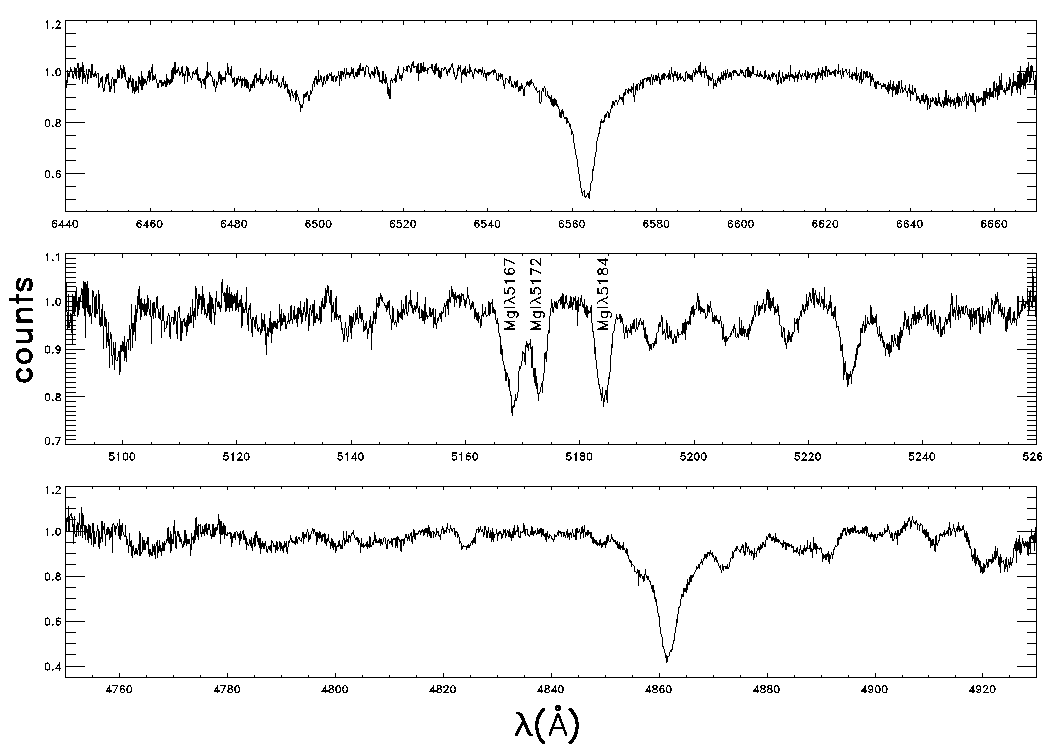
\includegraphics[width=1.\textwidth]{MES_spectrum.pdf}
	\caption[MES spectrum of a confirmed member of 25 Ori]{MES spectrum of a confirmed member of 25 Ori with a mass of 1.7 $M_\odot$. The panels show the absorption of the lines: H$_\alpha$ (in order 34; upper panel), MgI$\lambda\lambda\lambda$5167, 5172, 5184 (in order 43; middle panel) and H$_\beta$ (in order 46; lower panel).}
	\label{fig_MES:spectrum}
\end{figure*}

\subsubsection{Physical Parameters}
\label{sec_MES:phy_par}
%We expect to calculate the $T_{eff}$ of all the MES spectra using the SPTCLASS code to obtain the spectral types to then convert them to $T_{eff}$ using the \citet{Kenyon-Hartmann1995} or \citet{Pecaut2013} relations. 
We estimated $T_{eff}$ of the member candidates observed with MES by interpolating their observed $G-J$ colors from Gaia DR2 and 2MASS in an updated version of the \citet{Kenyon-Hartmann1995} relation, assuming the 25 Ori $A_V$ obtained in this work ($0.29\pm0.26$ mag). For the estimation of $L_{bol}$, mass and age we used the routine described in Section \ref{sec_APOGEE-2:physical_parameters}, working with the PARSEC-COLIBRI isochrones. The masses obtained for the sources range between 1.3 and 11 $M_\odot$.

%++++++++++++++++++++++++++++
\subsection{SDSS-IV/APOGEE-2 for Intermediate-mass Stars}
\label{sec:APOGEE-2}

\subsubsection{APOGEE-2 Spectra}
\label{sec_APOGEE-2:spectra}
In order to observe 25 Ori member candidates less massive that those observed with the MES spectrograph but more massive than the peak of the IMF (0.30 $M_\odot$; Su\'arez et al. 2018, submitted), we used the Apache Point Observatory Galactic Evolution Experiment 2 (\ac{APOGEE-2}) spectrograph, mounted on the 2.5m SDSS telescope \citep{Gunn2006,Blanton2017}. As one of the SDSS-IV programs, APOGEE-2 uses a multi-fiber spectrograph that allows the acquisition of up to 300 moderate-to-high resolution ($R\sim22500$) spectra at the $H$-band (1.51-1.70 $\mu$m) across a 1.5$^\circ$ radius circular FOV \citep{Wilson2010,Majewski2017}. We obtained the data as part of the APOGEE-2 Young Cluster Survey and divided into two high-priority fields with 10 visits dedicated to the observation of mainly 25 Ori targets. Our participation in this survey is thanks to the collaboration of UNAM in SDSS-IV. In Table \ref{tab:APOGEE-2_fields} we summarize the details of these APOGEE-2 fields in 25 Ori. %Each visit provided spectra for about 250 scientific targets.

\begin{table}[ht!] \tiny
\begin{center}
 \caption{APOGEE-2 fields in 25 Ori.}
 \label{tab:APOGEE-2_fields}
 \begin{threeparttable}
  	\setlength{\tabcolsep}{11pt}
	\begin{tabular}{lcccccc}
	\toprule
	{\bf Field Name} & {\bf RA}    & {\bf DEC}  & {\bf Plate ID} & {\bf Epoch} & {\bf UT Date}         & Seeing   \\
	                 & ($^\circ$) & ($^\circ$)  &                & (MJD)       & (yyyy-mm-ddThh:mm:ss) & (arcsec) \\
	\midrule
	Ori OB1ab-E & 81.496 & 1.006 & 8900 & 2457648 & 2016-09-17T11:01:08.967 & 1.4 \\
	            &        &       & 8901 & 2457649 & 2016-09-18T11:24:21.106 & 1.4 \\
	            &        &       & 8901 & 2457650 & 2016-09-19T11:22:07.462 & 1.4 \\
	            &        &       & 8902 & 2457652 & 2016-09-21T11:59:29.344 & 1.4 \\
	            &        &       & 8902 & 2457653 & 2016-09-22T11:10:54.354 & 1.8 \\
	            &        &       & 8903 & 2457675 & 2016-10-14T10:17:16.340 & 1.6 \\
	\midrule
	Ori OB1ab-F & 82.000 & 3.000 & 8904 & 2457676 & 2016-10-15T10:53:52.447 & 1.5 \\
	            &        &       & 8905 & 2457410 & 2016-01-23T04:27:33.611 & 1.5 \\
	            &        &       & 8906 & 2457411 & 2016-01-24T04:24:59.808 & 1.4 \\
	            &        &       & 8906 & 2457412 & 2016-01-25T04:55:00.687 & 2.1 \\
	\bottomrule
	\end{tabular}
%	\begin{tablenotes}[para,flushleft]
%	  $^a$ Less time than requested but the spectra have enough SNR for our analysis.\\
%	\end{tablenotes}
 \end{threeparttable}
\end{center}
\end{table}

\subsubsubsection{Target Selection}
\label{sec_APOGEE-2:targets}
The selection of the targets was based on IR excess, variability and color-magnitude criteria as well as including previously confirmed member and X-ray sources, as described in \citet{Cottle2018} and summarized as followed:

$i)$ For a uniform selection of young stellar objects (\ac{YSO}s) with IR excess, the \cite{Koenig2014} method was followed, considering NIR and mid-IR photometry from the 2MASS and WISE \citep{Cutri2013} catalogs, respectively, which provides an efficiency of about 80\%, proven in $\sigma$ Ori and $\lambda$ Ori \citep{Koenig2015}. 

$ii)$ Additionally, to extend the uniform selection of YSOs, including diskless sources, we considered variable candidates, which is an effective method for the selection of PMS stars \citep{Briceno2005,Briceno2018}, using the PanSTARRS catalog \citep{Chambers2016}. 

$iii)$ The number of YSOs selected from IR excess and variability criteria required to use about 10\% of the available APOGEE-2 fibers, therefore, we filled the rest of the fibers with previously confirmed members by \citet{Briceno2005,Briceno2007,Downes2014,Suarez2017} as well as highly probable member from \citet{Kharchenko2005}, X-ray sources from the 3XMM-DR5 catalog \citep{Rosen2015} and member candidates selected on the basis of their position in $I$ vs $I-J$ diagrams using photometry from the USNO \citep{Monet2003} and 2MASS catalogs. For the selection of the latter group of member candidates we considered the sources lying inside the defined PMS locus, working with the empirical isochrone traced by several spectroscopically confirmed members and highly probable members of 25 Ori and Orion OB1a. In Figure \ref{fig_APOGEE-2:targets_selection} we show the CMDs used for the selection of photometric candidates observed with APOGEE-2 in 25 Ori. 

In Table \ref{tab_APOGEE-2:targets} we summarize the number of APOGEE-2 targets selected from the above criteria and keeping all of them with $H$-band magnitudes between 7. and 12.2, in order to ensure signal-to-noise ratio (\ac{SNR}) $>100$ for a three-visit source with a total of 3h of exposure \citep{Majewski2017}. We prioritized the targets to first assign fibers to the uniformly selected sources and then to the rest of the candidates. After removing duplicates and 72'' fiber collisions, we acquired 1185 unique APOGEE-2 spectra in both fields dedicated to 25 Ori. In Figure \ref{fig_APOGEE-2:sky} we show the spatial distribution of these APOGEE-2 targets.

\begin{figure*}[ht!]
	\centering
	\begin{tabular}{cc}
		\subfloat{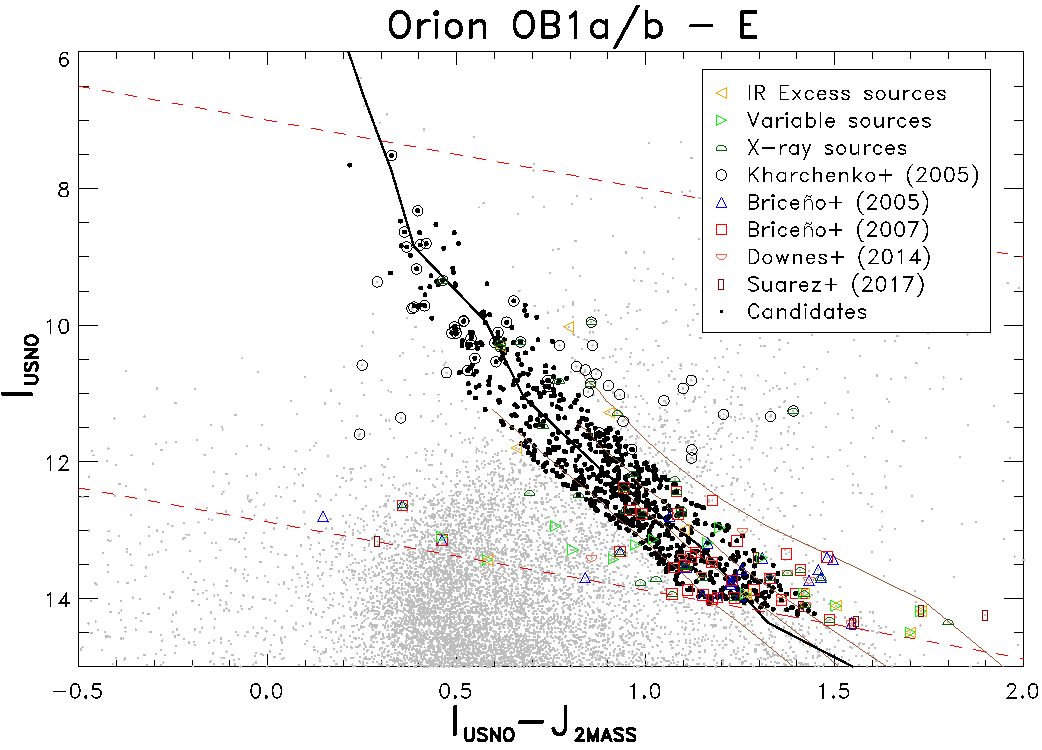
\includegraphics[width=.50\linewidth]{CMD_plate_E.pdf}} & 
		\subfloat{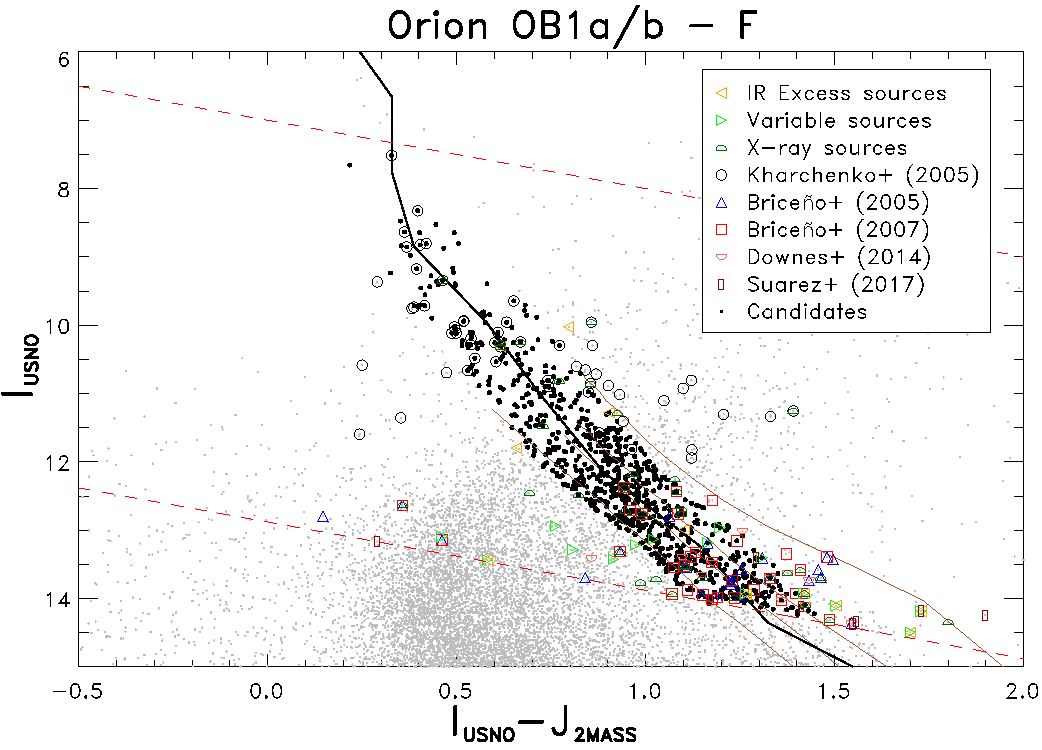
\includegraphics[width=.50\linewidth]{CMD_plate_F.pdf}}
	\end{tabular}
	\caption[CMD for the selection APOGEE-2 targets.]{CMDs used to select member candidates (black points) for the APOGEE-2 fields dedicated to 25 Ori (OB1ab-E in left panel and OB1ab-F in right panel). The open symbols show confirmed members, highly probable members and member candidates of 25 Ori and Orion OB1a, as indicated in the label. The black solid curve corresponds to the empirical isochrone and the brown curves represent the BT-Settl isochrones for 1, 3, 5 and 10 Myr. The red dashed lines indicate the APOGEE-2 limits of 7 and 12.2 mag in the $H$-band. These plots are based on those in \citet{Cottle2018}.
	\label{fig_APOGEE-2:targets_selection}}
\end{figure*}

\begin{table} \scriptsize
\begin{center}
 \caption{APOGEE-2 targets in 25 Ori.}
 \label{tab_APOGEE-2:targets}
 \begin{threeparttable}
  	%\setlength{\tabcolsep}{11pt}
	\begin{tabular}{@{\extracolsep{2pt}}cccccccccc}
	\toprule
	\multicolumn{2}{c}{{\bf IR Excess}} & \multicolumn{2}{c}{{\bf Variable}} & \multicolumn{2}{c}{{\bf X-ray sources}} & \multicolumn{2}{c}{{\bf Members}$^a$} & \multicolumn{2}{c}{{\bf Candidates}} \\
   	\cline{1-2}
   	\cline{3-4}
   	\cline{5-6}
   	\cline{7-8}
   	\cline{9-10}
	{\bf Selected} & {\bf Observed}     & {\bf Selected} & {\bf Observed}    & {\bf Selected} & {\bf Observed}         & {\bf Selected} & {\bf Observed}       & {\bf Selected} & {\bf Observed}      \\
	\midrule
	23 & 20 & 28 & 25 & 40 & 38 & 216 & 92 & 1442 & 985 \\
	\bottomrule
	\end{tabular}
	\begin{tablenotes}[para,flushleft]
	  $^a$ Spectroscopically confirmed members considering the studies by \citet{Briceno2005,Briceno2007,Downes2014,Suarez2017}.\\
	\end{tablenotes}
 \end{threeparttable}
\end{center}
\end{table}

\begin{figure*}%[ht!]
	\centering
	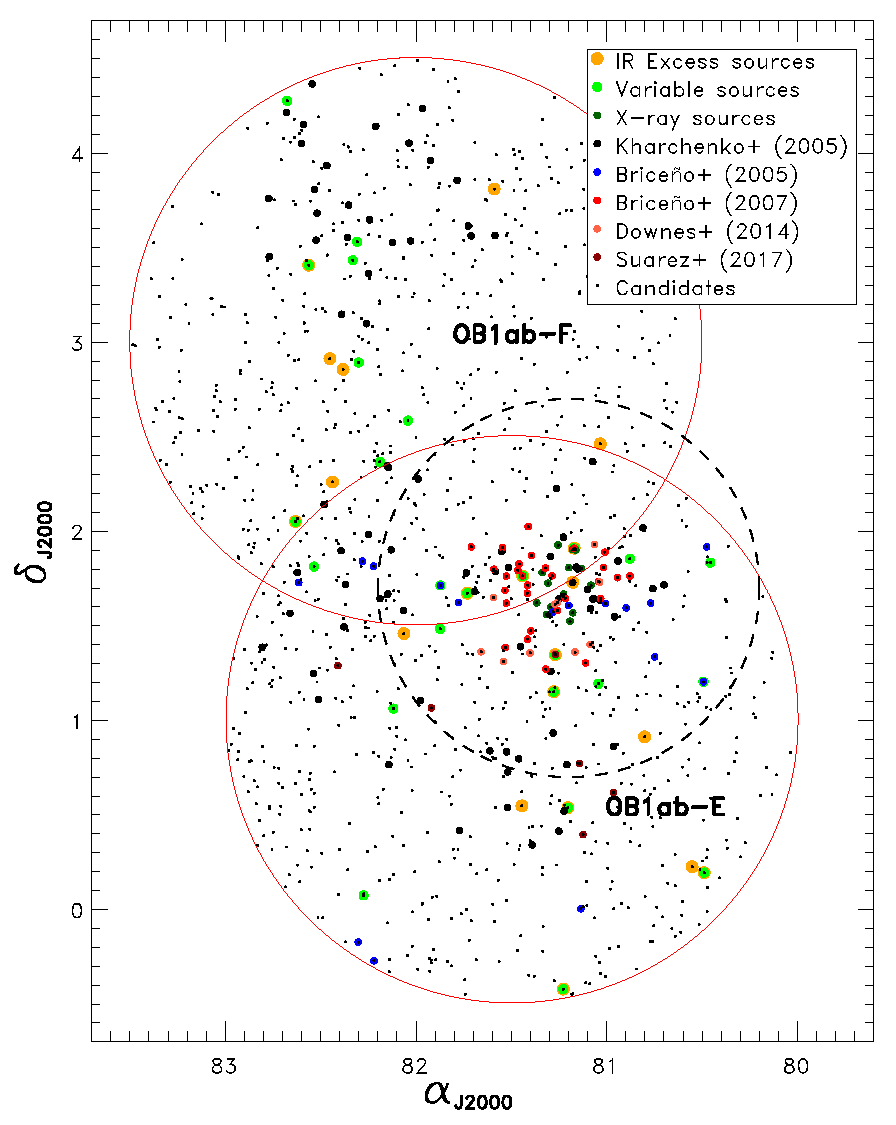
\includegraphics[width=1.\textwidth]{sky_APOGEE-2.pdf}
	\caption[Spatial distribution of the targets observed by APOGEE-2 in 25 Ori]{Spatial distribution of the targets observed by APOGEE-2 in the two fields dedicated to 25 Ori (red circles). The colored points represent the different kind of targets and the sizes indicate their priority, as shown in the label. The dashed circle shows the 1$^\circ$ radius area of 25 Ori.}
	\label{fig_APOGEE-2:sky}
\end{figure*}

\subsubsubsection{Radial Velocities and Effective Temperatures}
\label{sec_APOGEE-2:targets}
We retrieved the APOGEE-2 spectra from the Science Archive Sever (\ac{SAS}), which are available for SDSS-IV members. These spectra were originally processed by the APOGEE Stellar Parameter and Chemical Abundances Pipeline \citep[\ac{ASPCAP}; ][]{GarciaPerez2016}, which is an automated software for the determination of RV, $T_{eff}$, log $g$ and chemical abundances with accuracies of $\sim$0.1 km s$^{-1}$, 2\%, 0.1 dex and $\lesssim0.05$ dex, respectively, through a comparison of the observed spectra to libraries of theoretical spectra. However, ASPCAP is optimized for the analysis of spectra of red giant stars and can introduce biases when working with spectra of YSOs \citep{Nidever2015}. Therefore, these APOGEE-2 spectra were processed by \citet{Kounkel2018} using the pipeline developed by \citet{Cottaar2014}, which is designed for spectra of PMS stars. This pipeline determines the $T_{eff}$, log $g$, RV, rotational velocity ($v$ sin $i$) and $H$-band veiling ($r_H$) for each source by fitting the observed spectra to synthetic spectra and minimizing $\chi^2$. The corresponding uncertainties are derived by the pipeline using Markov chain Monte Carlo simulations. After some comparisons between the results using the \citet{Coelho2005}, \citet{Allard2012} and \citet[\ac{PHOENIX}; ][]{Husser2013} spectral libraries assuming solar metallicities, it was decided to adopt those from PHOENIX because produce the most self-consistent solutions and covers the widest $T_{eff}$ range (2300-15000 K) \citep{Kounkel2018}. These fits were done for each visit spectrum and then, the reported parameters for each target are the weighted average of the parameters in all the visits for that specific target. Additionally to the use of this pipeline, we are working with a new code named TONALLI (Adame et al. 2018, in preparation) to fit the PHOENIX synthetic spectra to the observed spectra considering $\alpha$ element (O, Ne, Mg, Si, S, Ar, Ca and Ti) abundance ([$\alpha/$Fe]) and [Fe/H] as additional free parameters. As this is still an ongoing work, for the analysis presented in this thesis we used the parameters derived by \citet{Kounkel2018}. 

Particularly, the parameters of interest for this project from the APOGEE-2 spectra are $T_{eff}$ and RV. For the APOGEE-2 fields in 25 Ori, the typical $T_{eff}$ uncertainties are 40 K but they significantly increase for sources with $T_{eff}>6250$ K. In the case of the RV errors, the typical values are 0.5 km s$^{-1}$.

\subsubsection{Spectra Analysis}
\label{sec_APOGEE-2:analysis}

\subsubsubsection{Membership Assignment}
\label{sec_APOGEE-2:memberships}
The APOGEE-2 targets selection was not totally impervious to contamination from background and, in a lesser degree, from foreground field stars. For this reason, in order to select the 25 Ori members we applied distance, RV and spatial distribution criteria, similarly to those used for the MES spectra in Section \ref{sec_MES:membership}, assuring consistent values with those expected for the 25 Ori population. About 90\% of all the targets in the Ori OB1ab-E and OB1ab-F fields have reliable BJ18 distances (errors less than 20\%) and there are 353 sources satisfying the distance and RV criteria, out of which 153 lie inside the 1$^\circ$ radius area of 25 Ori. This sample of 25 Ori members spans $H$-band mangitudes between 8.4 and 12.2. From these 153 members in 25 Ori, 56 of them were confirmed before through spectroscopic studies by \citet[18 sources; ][]{Briceno2005}, \citet[9 sources; ][]{Briceno2007}, \citet[8 sources; ][]{Downes2014}, \citet[3 sources; ][]{Suarez2017} and \citet[18 sources; ][]{Briceno2018}. All of these members have $H$-band magnitudes fainter than 10.6 (1.3 $M_\odot$). Therefore, we confirmed 97 new members of 25 Ori using APOGEE-2 spectra.
%, 97 new members of 25 Ori,% with masses $0.6\lesssim m/M_\odot \lesssim 3.7$.
%Additionally, 32 of our confirmed members have high-probability of being members according to \citet{Kharchenko2005}.

There are 9 additional previously confirmed 25 Ori members (2 from \citealt{Briceno2005}, 1 from \citealt{Briceno2007}, 1 from \citealt{Downes2014} and 5 from \citealt{Briceno2018}) with APOGEE-2 spectra that we did not recover after applying our membership criteria; 2 of them because they have distances of $180\pm2$ and $545\pm87$ pc and the remaining 7 members because they do not have Gaia DR2 parallaxes (4 sources) or their parallaxes or RVs have errors larger than 20\% (3 sources).

\subsubsubsection{Radial Velocity Dispersion}
\label{sec_APOGEE-2:rv_dispersion}
With the sample of confirmed members from the APOGEE-2 spectra, we analyzed their radial velocities to obtained the velocity dispersion (\ac{sigmaRV}). In Figure \ref{fig_APOGEE-2:rv} we show the radial velocity distributions of all the APOGEE-2 targets lying inside 25 Ori ($1^\circ$ radius area) and for the distance filtered targets as well as for the previously confirmed members. The most prominent peak corresponds to the 25 Ori population and has a mean value of $20.9\pm2.0$ km s$^{-1}$, considering the previously confirmed members with APOGEE-2 RVs or the APOGEE-2 targets filtered by their distances and removing those with RV larger than 28 km s$^{-1}$. This mean RV and velocity dispersion are very consistent with that obtained by \citet[$19.7\pm1.7$ km s$^{-1}$; ][ and references therein]{Briceno2007} working with a smaller sample of 47 members of 25 Ori. Also, the velocity dispersion is consistent with the typical value of 1-3 km s$^{-1}$ for a sample of 28 clusters and associations with ages of $\sim1-5$ Myr by \citet{Kuhn2018}. 

The velocity dispersion we obtained in this section supports the confirmation of 25 Ori as a gravitationally unbound association in Section \ref{sec_IMF:unbound}, when comparing its velocity dispersion with its escape velocity. With this velocity dispersion we also estimate that the crossing time, $t_{cross}=2r_{hm}/\sigma_{RV}$, of 25 Ori is $3.0$ Myr, considering a half-mass radius $r_{hm}\approx3$ pc, obtained from the system IMF we derived in Su\'arez et al. (2018, submitted). This crossing time corresponds to a relaxation time, $t_{relax}\simeq\frac{0.1N}{\textnormal{ln}N}t_{cross}$, of about 32 Myr. As the 25 Ori age is $\sim$7 Myr, this implies that the groups is dynamically young and has not had time enough to relax through interactions between the members.

Additionally in Figure \ref{fig_APOGEE-2:rv}, we observed a second peak at about 28 km s$^{-1}$ that can be due to the presence of dispersed OB1a population or even to overlapping members of OB1b \citep[Orion C and D; ][]{Kounkel2018}, which have RVs of $\sim24$ \citep{Jeffries2006} and $30.1\pm1.9$ km s$^{-1}$ \citep{Briceno2007}, respectively.

\begin{figure*}[ht!]
	\centering
	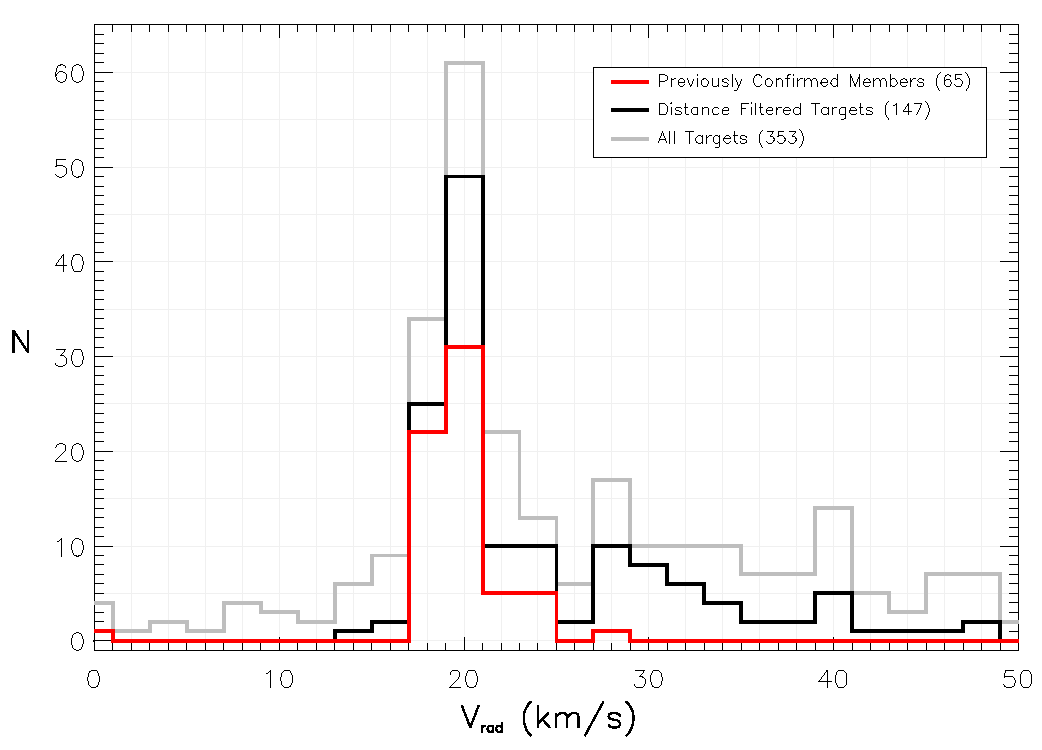
\includegraphics[width=1.\textwidth]{radial_velocity.pdf}
	\caption[Radial velocity distributions of the APOGEE-2 targets and members of 25 Ori.]{Radial velocity distributions of all the APOGEE-2 targets inside 25 Ori (gray histogram), of the targets after applying the distance criterion (black histogram) and of the spectroscopically confirmed members in the literature with RV from APOGEE-2 (red histogram).}
	\label{fig_APOGEE-2:rv}
\end{figure*}

\subsubsubsection{Physical Parameters}
\label{sec_APOGEE-2:physical_parameters}
After we applied the membership criteria to the APOGEE-2 spectra in the OB1ab-E and OB1ab-F fields, we estimated the physical parameters of interest for the resulting 25 Ori members. For this purpose, we developed a custom computer program, which we describe below.

\paragraph{PHYPAR Routine\\}
\label{sec_APOGEE-2:phypar}
For the estimation of the bolometric luminosity (\ac{Lbol}), mass and age of young stellar and substellar objects, I developed the PHYPAR IDL routine (see Appendix \ref{sec_app:phypar}), which has been succesfully used in several contributions \citep{Suarez2017,Kounkel2018,Ramirez-Preciado2018}. The input parameters are distance, $T_{eff}$, $A_V$, and a photometric band magnitude together with their uncertainties. So far, the code works with magnitudes in the $G$, $V$, $R$, $I$, $J$, $H$ or $K$ photometric bands.

First, the magnitudes are dereddened using the input $A_V$ and assuming the \citet{Cardelli1989} coefficients for all the photometric bands less that from Gaia or the coefficient $C_G=0.9145$ (J. Hern\'andez, private communication) for the $G$ magnitudes. Then, the distance modulus is added to the dereddened magnitudes to obtain the absolute magnitudes. These magnitudes are then converted to bolometric magnitudes using the bolometric corrections obtained by interpolating $T_{eff}$ in the \citet{Kenyon-Hartmann1995} relation combined with the \citet{Luhman1999}, \citet{Briceno2002} and \citet{Luhman2003b} relations for the LMSs and BDs. Then, the bolemetric magnitudes are converted to $L_{bol}$. Finally, $T_{eff}$ and $L_{bol}$ are interpolated into stellar evolution models to obtain masses and ages for the sources lying inside a defined region of the model grid. This region is defined according to the expected masses and ages of the sources, which avoids degeneracy when the stellar model also includes post-MS stages. The code uses the BT-Settl or PARSEC-COLIBRI isochrones, which allows to cover a wide mass range (from planetary masses to tend of solar masses) for sources in the PMS or MS.

The errors for each parameter are obtained as follows: $i)$ when each of the above steps involve an equation, the uncertainties are computed by using the corresponding error propagation rule and $ii)$ when an interpolation is done, the error is defined as the standard deviation of the resultant values from the interpolation of 10$^3$ artificially generated numbers drawn from a normal distribution centered at the parameter value and with a standard deviation equal to one third its error (this way 99.7\% of the random values are within the uncertainties).

%{\href{https://drive.google.com/open?id=1uNv7nxVas2F0TOz3q5aJsKD8yVd4FwqG}{\texttt{PHYPAR}}} IDL routine I developed, which has been succesfully tested in several contributions \citep{Suarez2017,Kounkel2018,Ramirez-Preciado2018}. The input parameters are distance, $T_{eff}$, $A_V$, and a photometric band magnitude together with their uncertainties. First, the magnitudes are dereddened by assuming the \citet{Cardelli1989} coefficients for the 2MASS photometric bands and the above mentioned Gaia coefficient to then add the distance modulus to obtain the absolute magnitudes. These magnitudes are converted to bolometric magnitudes using the bolometric corrections (BCs) obtained by interpolating $T_{eff}$ in the \citet{Kenyon-Hartmann1995} relation and then are converted to $L_{bol}$. Finally, $T_{eff}$ and $L_{bol}$ are interpolated into stellar models to obtain masses and ages for the members lying inside a defined region of the models. The errors for each parameter are obtained as follow: $i)$ when each of the above steps involve an equation, the uncertainties are computed using the corresponding error propagation rule and $ii)$ when an interpolation is done, the error is defined as the standard deviation of the resultant values from the interpolation of 10$^3$ generated numbers following a normal distribution centered at the parameter value and with a standard deviation equal to one third its error (this way 99.7\% of the random values are within the uncertainties). So far, the code works with magnitudes in the $V$, $G$, $J$, $H$ or $K$ photometric bands and with the BT-Settl or PARSEC-COLIBRI isochrones.

\paragraph{Parameters\\}
\label{sec_APOGEE-2:parameters}
Before using the PHYPAR code for the resulting confirmed members, we estimated $A_V$ by using photometry from the Gaia DR2 and 2MASS catalogs and $T_{eff}$ from the APOGEE-2 spectra. We compared the observed $G-J$ and $G_{BP}-G_{RP}$ colors with the intrinsic colors obtained by interpolating $T_{eff}$ into the PARSEC-COLIBRI 7 Myr isochrone and then transforming the color excesses to $A_V$. When this resulted into a negative extinction, which can be due to the $T_{eff}$ errors and/or magnitude uncertainties, we assigned null values. We computed the $A_V$ uncertainties with the same method describe in Section \ref{sec_APOGEE-2:phypar}. For most of the sources, the $A_V$ values obtained using only Gaia DR2 photometry are in agreement with those combining Gaia DR2 with 2MASS. The resultant $A_V$ from the Gaia DR2 photometry are lower than 1.8 mag, but most of them ($\approx$75\%) have values lesser than 1 mag. The mean extinction, \ac{mAv}, we obtained is $0.39\pm0.40$ mag, considering sources with values lower than 1 mag. This low extinction is consistent with previous works (Su\'arez et al. 2018, submitted and references therein).
%assuming the coefficients $C_{G_{BP}}=1.039$, $C_G=0.9145$, $C_{G_{RP}}=0.601$ and $C_J=0.282$ (\citealt{Cardelli1989} and J. Hern\'andez, private communication)

Then, the $L_{bol}$, mass and age of the APOGEE-2 members were obtained using the PHYPAR routine with distances from BJ18, $T_{eff}$ from the APOGEE-2 spectra, $A_V$ derived here from the Gaia DR2 photometry and $G$ magnitudes from Gaia DR2 as well as the PARSEC-COLIBRI isochrones. In Figure \ref{fig_APOGEE-2:HR} we show the H-R diagram of the members from the APOGEE-2 spectra. The masses of these members in 25 Ori ranges between 0.3 and 5.2 $M_\odot$. The mean age we obtained is $7.2\pm3.6$ Myr, which is very consistent with previous studies in 25 Ori \citep[][ and references therein]{Briceno2018}.

\begin{figure*}[ht!]
	\centering
	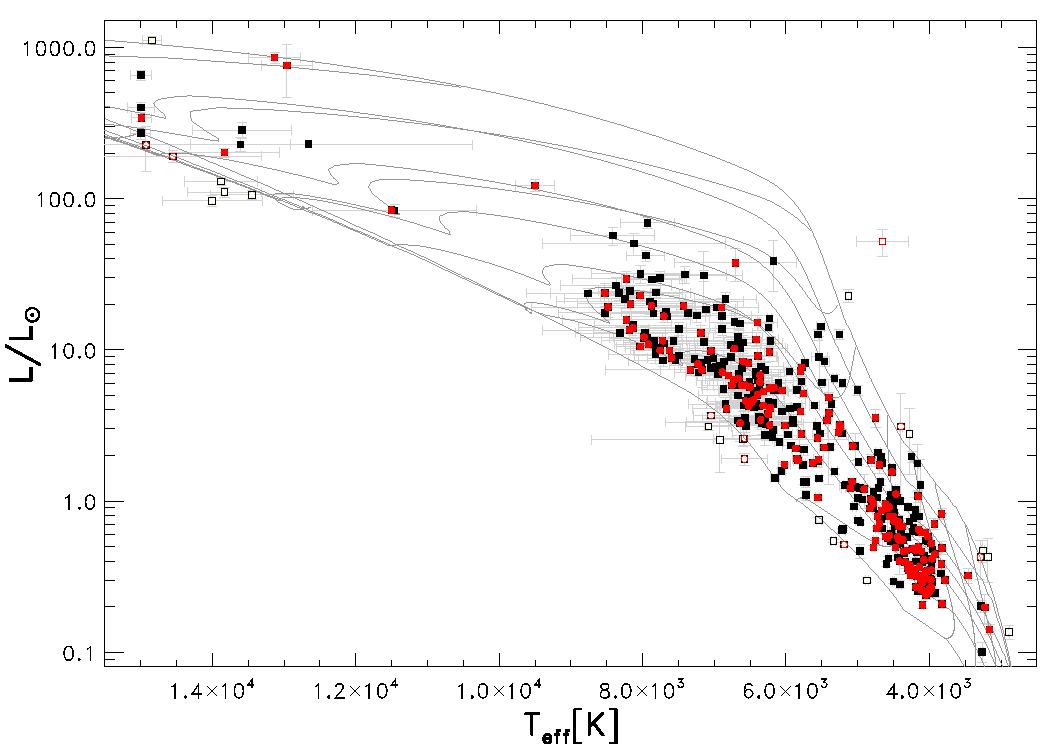
\includegraphics[width=1.\textwidth]{HR_APOGEE-2.pdf}
	\caption[H-R diagram of the 25 Ori confirmed members from APOGEE-2 spectra.]{H-R diagram of the confirmed members in the APOGEE-2 OB1ab-E and OB1ab-F fields (black squares) and of the members lying inside the 25 Ori area of $1^\circ$ radius (red circles). The gray curves represent the PARSEC evolutionary tracks for 0.3, 0.5, 0.7, 1.0, 2.0, 3.0, 4.0 and 5.0 $M_\odot$ and the PARSEC-COLIBRI isochrones for 0.5, 1, 2, 3, 5, 10 and 30 Myr. The open symbols indicate the members without mass and age estimates because they lie outside the model grid.}
	\label{fig_APOGEE-2:HR}
\end{figure*}

\subsection[SDSS-III/BOSS for Low-mass Stars]{SDSS-III/BOSS for Low-mass Stars \citep{Suarez2017}}
\label{sec:BOSS}
The following analysis constitutes the publication ``New Low-Mass Stars in the 25 Orionis Stellar Group and Orion OB1a Sub-association from SDSS-III/BOSS Spectroscopy'' by \citet{Suarez2017}, which was carried out as part of this dissertation.

%\begin{figure*}[ht!]
%	\centering
%	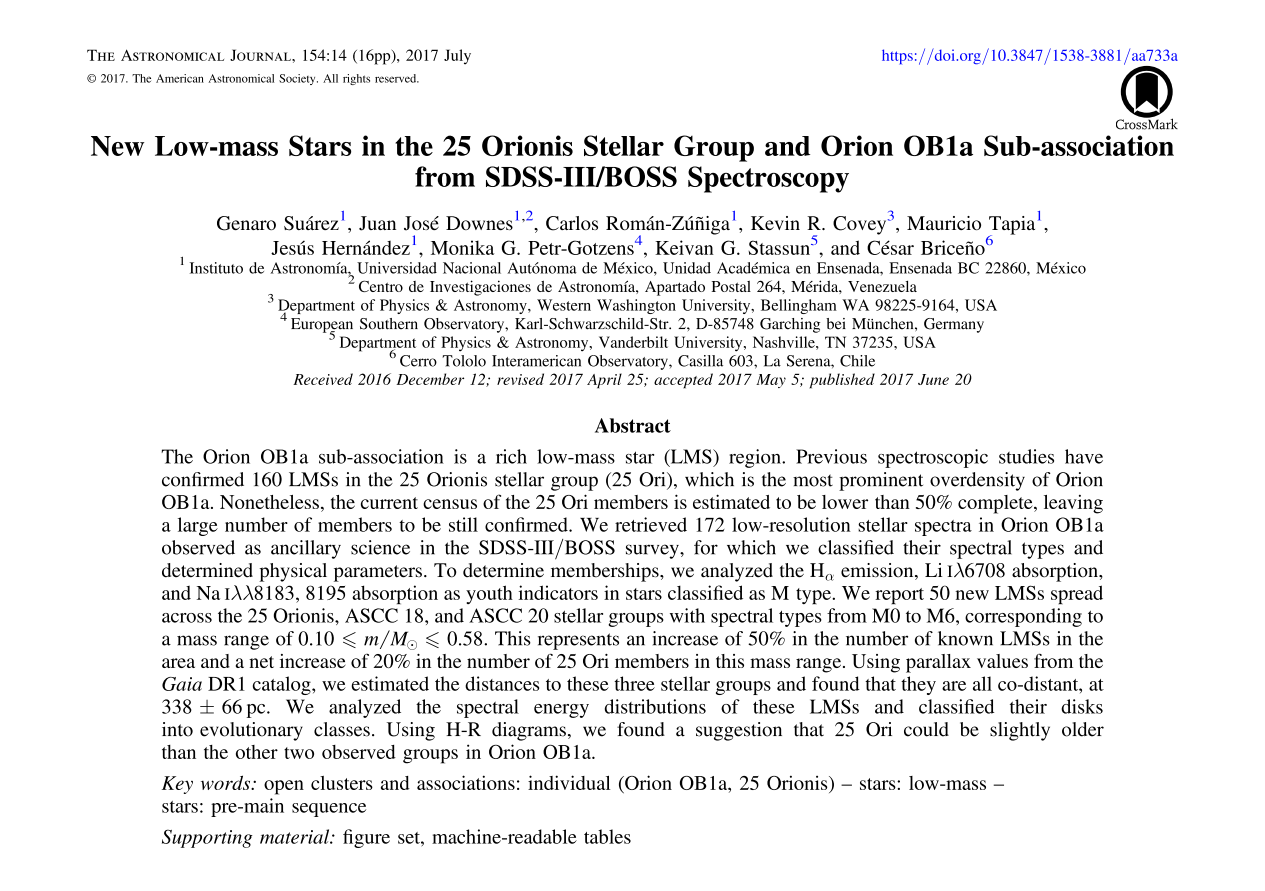
\includegraphics[width=1.\textwidth]{BOSS_paper.png}
%	\caption[]{.}
%	\label{fig_BOSS:paper}
%\end{figure*}

{\bf Abstract.}
The Orion OB1a sub-association is a rich low mass star (LMS) region. Previous spectroscopic studies have confirmed 160 LMSs in the 25 Orionis stellar group (25 Ori), which is the most prominent overdensity of Orion OB1a. Nonetheless, the current census of the 25 Ori members is estimated to be less than 50\% complete, leaving a large number of members to be still confirmed. We retrieved 172 low-resolution stellar spectra in Orion OB1a observed as ancillary science in the SDSS-III/BOSS survey, for which we classified their spectral types and determined physical parameters. To determine memberships, we analyzed the H$_\alpha$ emission, LiI$\lambda$6708 absorption, and NaI$\lambda\lambda$8183, 8195 absorption as youth indicators in stars classified as M-type. We report 50 new LMSs spread across the 25 Orionis, ASCC 18, and ASCC 20 stellar groups with spectral types from M0 to M6, corresponding to a mass range of 0.10$\le m/\textrm{M}_\odot \le$0.58. This represents an increase of 50\% in the number of known LMSs in the area and a net increase of 20\% in the number of 25 Ori members in this mass range. Using parallax values from the Gaia DR1 catalog, we estimated the distances to these three stellar groups and found that they are all co-distant, at 338$\pm$66 pc. We analyzed the spectral energy distributions of these LMSs and classified their disks by evolutionary classes. Using H-R diagrams, we found a suggestion that 25 Ori could be slightly older that the other two observed groups in Orion OB1a.

\subsubsection{Introduction}
\label{sec_BOSS:intro}
Comprehensive studies of known OB associations in terms of their stellar populations and structural properties provide a firm basis to the understanding of how young star aggregations form and evolve until they eventually disperse to be part of the Galactic disk component. Particularly useful in this respect are the $\sim 10$ Myr {\it fossil star forming regions} \citep[\ac{FSFR}s; ][]{Blaauw1991}, where one would expect that: \textit{i}) the dust and gas are largely dispersed, and extinction is generally low, permitting the detection of low mass stars (LMSs), \textit{ii}) the members are still spatially concentrated and can be distinguished from the field population, \textit{iii}) only a minority of stars retain optically thick circumstellar disks, \textit{iv}) the active star formation was ceased but its products are still present, \textit{v}) accretion is essentially over, so the objects have attained their final masses, and \textit{vi}) the stars can be considered nearly coeval.

The properties of the LMSs in the FSFRs are of particular importance to understand/clarify the structure and dispersal processes acting on such stellar populations, the circumstellar disk evolution and the possible large-scale dynamical effects. In fact, such studies are not possible solely from the observation of massive stars, as the LMSs do have relatively large PMS phases, they are characterized by the presence of evolving disks, variable mass accretion and circumstellar and chromospheric activity. Furthermore, they make up the majority of all the stars formed in clusters in terms of number and mass \citep[e.g.,][]{Bastian2010}, and have long lifetimes ($>10^{10}$ yr) in the MS.

The Orion OB1 association is one of the largest and nearest star forming regions \citep[e.g. ][]{Genzel-Stutzki1989,Bally2008,Briceno2008} and contains four distinct sub-associations, which can be distinguished according to their ages and content of gas and dust \citep{Blaauw1964}. With an age of 7-10 Myr and a distance of $\sim$330 pc \citep[e.g.,][]{Briceno2005}, Orion OB1a is the oldest and closest of the Orion OB1 sub-associations. Considering the critical age of 10 Myr, Orion OB1a is an excellent region for studying the early evolution of LMSs. Particularly important is the 25 Orionis stellar group (25 Ori), one of the most numerous and spatially dense 7-10 Myr old populations (r$\sim7$ pc, $\Sigma \sim 128$ stars deg$^{-2}$) known within 500 pc from the Sun \citep{Briceno2007}. 

As mentioned in \citet{Downes2014}, there are other associations of similar age to 25 Ori, but these regions cover relatively extended areas in the sky or are too distant to enable the detection of their LMSs. 25 Ori's unique combination of its distance, age, and area in the sky \citep[360 pc, $\sim7$ Myr, and $\approx 3$ deg$^2$; ][]{Briceno2005,Briceno2007,Downes2014}, makes it a particularly convenient region for studying the population of LMSs. Additionally, 25 Ori is almost free of extinction \citep[$A_V\approx0.30$ mag.; ][]{Kharchenko2005,Briceno2005,Briceno2007,Downes2014}.

Although 25 Ori is a clear spatial overdensity of young LMSs \citep{Briceno2007,Downes2014}, a level of contamination is expected close to 25 Ori from at least two other nearby 10 Myr old stellar groups, identified as ASCC 18 and ASCC 20 by \citet{Kharchenko2005,Kharchenko2013}. Thus, in order to disentangle these groups and identify the complete 25 Ori population, it is necessary to make a study that covers an area into those additional groups, beyond the proposed 25 Ori radius of $1^\circ$ \citep{Briceno2005,Briceno2007}.

Several spectroscopic studies have confirmed, to date, 160 LMS members of 25 Ori \citep{Briceno2005,Briceno2007,Biazzo2011,Downes2014,Downes2015}, which represent about 34\% of its total estimated LMS members \citep{Downes2014}. In this paper, we analyze optical spectra obtained with the SDSS-III/BOSS spectrograph to confirm 50 additional young LMSs in Orion OB1a, of which 22 are inside the 25 Ori's estimated area \citep[$1^\circ$ radius; ][]{Briceno2005,Briceno2007}. This increases the confirmed member sample of 25 Ori by about 20\% in a mass range from 0.1 to 0.6 M$_\odot$. We characterize these new members according to their optical spectral types and spectral features, as well as infrared (IR) photometric signatures of circumstellar disks. The paper is organized as follows: In Section \ref{sec_BOSS:observations} we describe the optical and IR photometric data, and the optical spectroscopy from the SDSS-III/BOSS survey. In Section \ref{sec_BOSS:results} we analyze the spectra and describe our results. In Section \ref{sec_BOSS:singular} we comment on particular objects and in Section \ref{sec_BOSS:summary} we discuss and summarize the results.

\subsubsection{Observations}
\label{sec_BOSS:observations}

\subsubsubsection{Optical Photometry}
\label{sec_BOSS:Optphot}
The $V$, $R$, and $I$ photometry used in this work was obtained from the CIDA Deep Survey of Orion (CDSO) catalog \citep{Downes2014}, which was constructed by co-adding the multi-epoch optical observations from the CIDA Variability Survey of Orion \citep[CVSO; ][]{Briceno2005,Mateu2012}. The sensitivity limits of the CDSO covers the LMS and brown dwarf (BD) population of 25 Ori and its surroundings within the region $79.7^\circ\lesssim\alpha\lesssim82.7^\circ$ and $0.35^\circ\lesssim\delta\lesssim3.35^\circ$. The limiting magnitude of the CDSO photometry in this region is $I_{lim}=22$ and the completeness magnitude is $I_{com}=19.6$ \citep{Downes2014}, enough to assure an $I$ band detection even for the faintest targets of our spectroscopic sample ($I\approx17.0$).

Additionally, we used the $u$, $g$, $r$, $i$, and $z$ photometry from the Sloan Digital Sky Survey (SDSS) catalog \citep[][]{Finkbeiner2004,Ahn2012}. These values are listed in Table \ref{tab_BOSS:photometry}.

\subsubsubsection{IR Photometry}
\label{sec_BOSS:IRphot}
The \textit{Z, Y, J, H,} and \textit{Ks} near-IR photometry used in this study was carried out by \citet{Petr-Gotzens2011} as part of the Visible and Infrared Survey Telescope for Astronomy \citep[VISTA; ][]{Emerson2004} science verification surveys \citep{Arnaboldi2010}. The 5$\sigma$ limiting magnitudes of the VISTA survey of the Orion star-forming region are $Z=22.5$, $Y=21.2$, $J=20.4$, $H=19.4$, and $Ks=18.6$, which are enough to have VISTA photometry even for the faintest objects in our spectroscopic sample ($J\approx15.0$).

Additionally, we used near-IR photometry from the 2MASS catalog \citep{Skrutskie2006} and mid-IR photometry from IRAC-\textit{Spitzer} \citep[][]{Hernandez2007b} and the \ac{WISE} (Wide-field Infrared Survey Explorer) All-Sky catalog \citep{Cutri2013}. This IR photometry is listed in Table \ref{tab_BOSS:photometry}.

\subsubsubsection{Spectroscopy}
\label{sec_BOSS:spectroscopy}
The spectra used in this paper were obtained as part of the Baryon Oscillation Spectroscopic Survey \citep[\ac{BOSS}; ][]{Dawson2013}, which is one of the four main surveys of SDSS \citep[][]{York2000} in its third phase \citep[SDSS-III; ][]{Eisenstein2011}. The BOSS spectrograph has plates with 1000 fibers of 2'' diameter spanning a field of view of 3.0$^\circ$ in diameter and cover a wavelength range from 3560 \AA\ to 10400 \AA\ with a resolution of R=1560 at 3700 \AA\ and R=2650 at 9000 \AA \citep{Gunn2006,Smee2013}. 

The spectra we analyzed were obtained as part of the {\it Star Formation in the Orion and Taurus Molecular Clouds} ancillary science program \citep{Alam2015}. The plate is centered around the B2 star 25 Orionis ($\alpha_{J2000}= 5^{\rm h} 24^{\rm m} 44^{\rm s}$.8; $\delta_{J2000} = +1^{\circ} 50' 47''.2$) and includes the stellar groups ASCC 16 (25 Ori), ASCC 18, and ASCC 20 \citep{Kharchenko2013}. The object selection process for this plate is described in detail in Section A2 by \citet{Alam2015} and is based on the cataloged optical and IR photometric properties (SDSS, WISE, 2MASS, Spitzer) of the objects. The integration time for the selected objects was 5 x 4500 s, achieving a typical S/N ratio of $\sim$20 for the faintest sources. The observation produced 677 spectra of which only 172 are stellar and the remaining 505 turned out to be spectra of galaxies and quasars, as explained in Section \ref{sec_BOSS:results}. In Figure \ref{fig_BOSS:sky} we show the spatial distribution of the targets observed in this plate \citep{Alam2015}, as well as the locations of the different stellar groups from \citet{Kharchenko2013}. In Figure \ref{fig_BOSS:CCD_bias} we show the $u-K$ vs $K$-W3 color-color diagram including all the targets of the 25 Ori BOSS plate, where we can see that most of these targets have $K$-W3 colors redder than those expected from previously confirmed members. It is important to notice that this target selection implies a bias towards sources with IR excesses (e.g. stars with accretion disks, see Section \ref{sec_BOSS:TTSclass}).

\begin{figure*}[ht!]
	\centering
	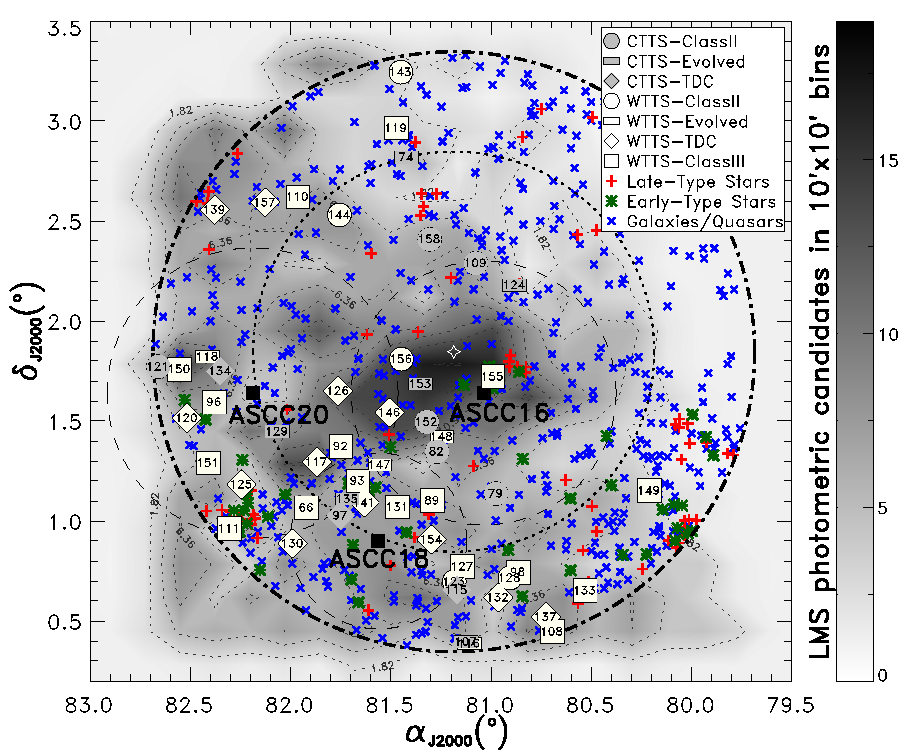
\includegraphics[width=1.\textwidth]{f1.pdf}
	\caption[Spatial distribution of the targets in the 25 Ori BOSS plate]{Spatial distribution of the confirmed members of 25 Ori or Orion OB1a classified as CTTSs and WTTSs on the BOSS plate dedicated to 25 Ori (thick dashed-dotted circle); see Sections \ref{sec_BOSS:memberships} and \ref{sec_BOSS:TTSclass}. The labeled circles, horizontal bars, diamonds, and squares represent YSOs classified as Class II objects, evolved systems, TDC or Class III objects, respectively, as shown in the label box (see Section \ref{sec_BOSS:SED}). The dotted circle represents the estimated area of 25 Ori \citep[1$^\circ$ radius; ][]{Briceno2005,Briceno2007}. The red plus signs, green asterisks, and blue cross signs indicate, respectively, stars later than G spectral type, G-type or earlier stars, and the galaxy/quasar samples. The black filled squares and the dashed circles around them represent, respectively, the central position and estimated area of the labeled stellar groups from \citet{Kharchenko2013}. The gray background map and the labeled isocontours indicate the LMS and BD photometric candidate density in 10'x10' bins from \cite{Downes2014}. The white star sign at the center represents the position of the 25 Orionis star.}
	\label{fig_BOSS:sky}
\end{figure*}

\begin{figure*}[ht!]
	\centering
	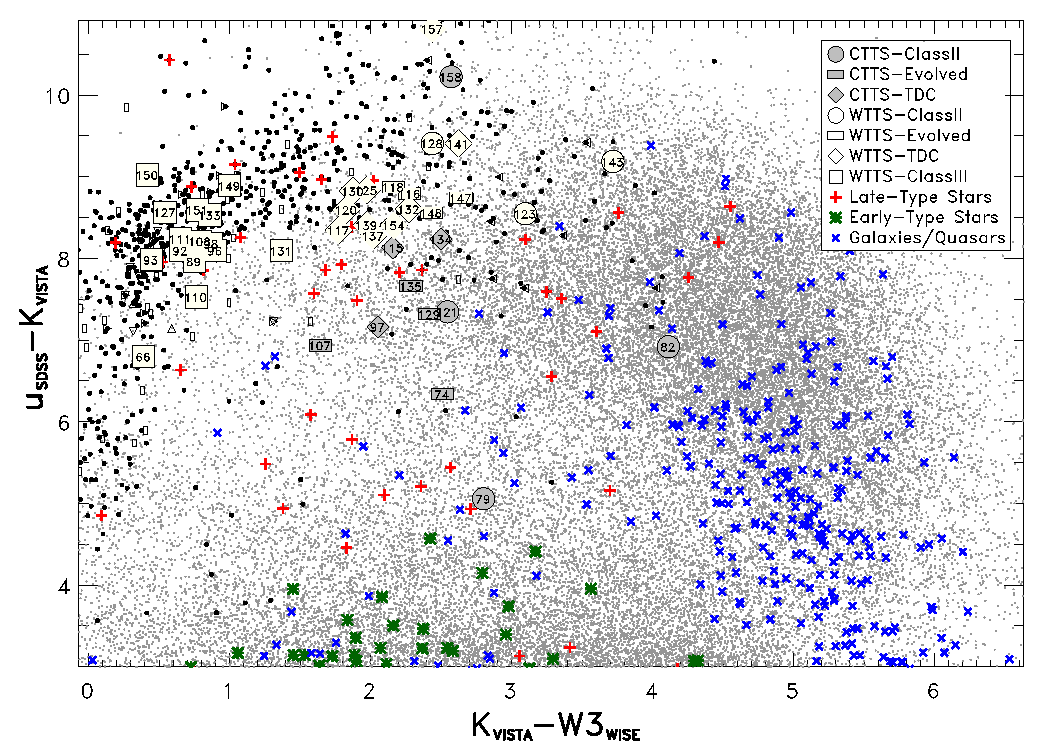
\includegraphics[width=1.\textwidth]{f2.pdf}
	\caption[Color-color diagram of the targets in the 25 Ori BOSS plate]{Color-color diagram showing the targets observed in the 25 Ori BOSS plate. The open upward triangles, downward triangles, rightfacing triangles, leftfacing triangles, and vertical bars indicate, respectively, previously confirmed members by \citet{Briceno2005,  Briceno2007, Downes2014, Downes2015, Briceno2018}. The black points represent the LMS and BD photometric candidates from \citet{Downes2014}, which were selected with an efficiency of $\sim 86\%$ from color-magnitude diagrams where a bias toward sources with IR excesses is not expected. The gray points show the SDSS+VISTA+WISE detections in the 25 Ori BOSS plate field of view. The rest of the symbols are indicated in the label. Note that the gray labeled symbols represent young stars showing intense H$_\alpha$ emission, as explained in Section \ref{sec_BOSS:TTSclass}.}
	\label{fig_BOSS:CCD_bias}
\end{figure*}

The BOSS ancillary science programs made use of the \texttt{v5\_7\_2} version of the \texttt{idlspec2d} pipeline, which, together with \texttt{idlutils}, are the SDSS pipelines used for the data reduction\footnote {\emph{\footnotesize SDSS data processing software is publicly available at \url{http://www.sdss.org/dr12/software/products/}}}. A detailed explanation of the automated classification and the redshift measurements was provided by \citet{Bolton2012}.

The calibrated wavelengths of the BOSS spectra are in the vacuum reference. In order to recognize spectral lines and to use stellar templates to analyze the BOSS spectra, it is needed to convert wavelengths from vacuum to air. We used the IAU standard transformations, as given in \citet{Morton1991}.

\subsubsection{Analysis and Results}
\label{sec_BOSS:results}
In Figure \ref{fig_BOSS:IvsI-J} we show the $I$ vs $I-J$ color-magnitude diagram for all the targets of the 25 Ori BOSS plate, together with the confirmed members in 25 Ori and Orion OB1a from \citet[][]{Briceno2005, Briceno2007, Downes2014, Downes2015}. We also included the 25 Ori members from \citet{Briceno2018}, which were selected according to their position in optical-near-IR color-magnitude diagrams and confirmed on the basis of youth indicators (e.g. H$_\alpha$ emission and NaI$\lambda6708$ absorption) and radial velocities, when available. Additionally, we included the photometric candidates from \citet{Hernandez2007b, Downes2014}. In this diagram, the confirmed members form a very clear locus, nicely separated from the Galactic disk dwarf stars and giant star branches, as well as from extragalactic sources. This shows that the combination of optical and near-IR photometry in color-magnitude diagrams allow for a clear selection of photometric candidates in regions like Orion OB1a \citep[e.g.,][]{Downes2014}.

\begin{figure*}[ht!]
	\centering
	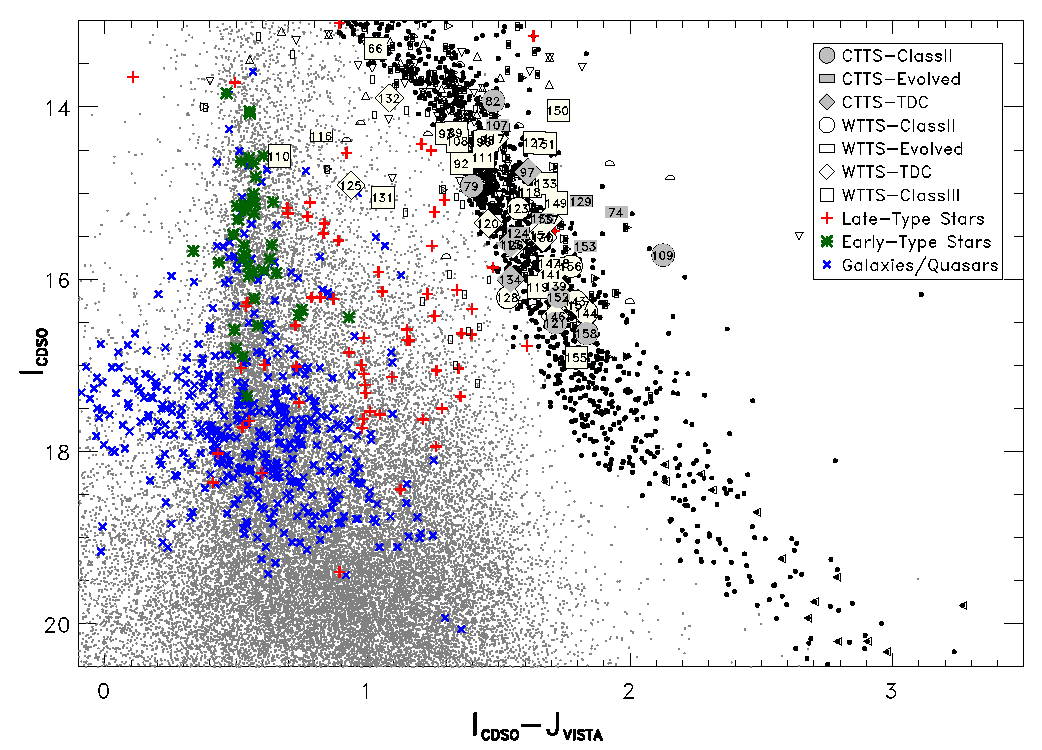
\includegraphics[width=1.\textwidth]{f3.pdf}
	\caption[Color-magnitude diagram of the targets in the 25 Ori BOSS plate]{Color-magnitude diagram from the CDSO and VISTA catalogs. The black points and open small symbols are as in Figure \ref{fig_BOSS:CCD_bias}. The open half circles represent the photometric candidates from \citet{Hernandez2007b}. The gray points show the CDSO+VISTA detections in the 25 Ori BOSS plate field of view. The rest of the symbols are indicated in the label.}
	\label{fig_BOSS:IvsI-J}
\end{figure*}

The BOSS spectra in the DR12 archive are provided with a spectral classification as well as an object classification (star, galaxy or quasar). The stellar templates used for this automated classification are mainly selected from The Indo-US Library \citep{Valdes2004}, which is focused on F- and early G-type stars. The library was supplemented for cool stars by theoretical atmosphere models computed using the MARCS models \citep{Gustafsson2008}. The M-type stellar templates in the database are representative of giant stars with effective temperature down to 3000 K, and a grid resolution of 500 K \citep{Palacios2010}. Thus, these templates are generally not suitable for the spectral type classification of young dwarf stars. Also, the grid resolution in effective temperature of the templates is not enough for the diversity of M-type stars present in our sample. Thus, to determine accurate physical parameters for the BOSS stars (extinction, effective temperature, bolometric luminosity, age, and mass), it is important to verify the SDSS spectral type classification independently. We visually inspected all spectra on the 25 Ori BOSS plate, confirming all objects correctly classified as stars by SDSS, and also identifying those sources for which the SDSS classification was incorrect, either stars classified as galaxies or quasars or, conversely, galaxies or quasars as stars. Through this process, we found 172 stellar spectra out of a total of 677 targets observed on the 25 Ori BOSS plate. The 505 remaining spectra from this plate correspond to either galaxies or quasars, as shown in Figure \ref{fig_BOSS:sky}.

%\floattable
\begin{table*} \scriptsize
 \caption[Photometric catalog of the confirmed members from the BOSS spectra]{Photometric catalog of the confirmed members of 25 Ori or Orion OB1a.}
 \label{tab_BOSS:photometry}
 \begin{threeparttable}
  \setlength{\tabcolsep}{12pt}
  %\renewcommand{\arraystretch}{1.5}
  \begin{tabular}{@{\extracolsep{2pt}}ccccccccccc@{}}
	\toprule
	{\bf ID} & {\bf $\alpha_{J2000}$} & $\delta_{J2000}$ & \multicolumn{5}{c}{{\bf SDSS}} & \multicolumn{3}{c}{{\bf CDSO}} \\
   	\cline{4-8}
   	\cline{9-11}
	& & & $u$ & $g$ & $r$ & $i$ & $z$ & $V$    & $R$    & $I$ \\
	\midrule
 	66  & 81.919314 & 1.065933 & 18.281    & 15.971    & 14.664    & 14.256    & 13.48     & 15.194 & 14.336 & 13.318 \\
  	74  & 81.421671 & 2.818307 & 18.326    & 17.989    & 17.294    & 16.394    & 15.679    & 17.935 & 16.772 & 15.223 \\
  	79  & 80.975436 & 1.136898 & 17.565    & 17.46     & 16.39     & 15.777    & 15.051    & 16.832 & 15.932 & 14.917 \\
  	82  & 81.269534 & 1.347489 & 18.175    & 17.499    & 16.287    & 15.147    & 14.329    & 16.621 & 15.302 & 13.93  \\
  	89  & 81.292164 & 1.102412 & 20.133    & 17.362    & 16.228    & 15.094    & 14.409    & 16.829 & 15.738 & 14.297 \\
  	92  & 81.747728 & 1.373077 & 20.591    & 18.091    & 16.675    & 15.412    & 14.743    & 17.287 & 16.203 & 14.657 \\
  	93  & 81.664785 & 1.200688 & 20.171    & 17.681    & 16.272    & 15.092    & 14.445    & 16.878 & 15.789 & 14.309 \\
  	96  & 82.379687 & 1.594114 & 20.233    & 17.702    & 16.291    & 15.081    & 14.415    & 16.926 & 15.903 & 14.404 \\
  	97  & 81.75054  & 1.026903 & 19.279    & 18.115    & 16.778    & 15.467    & 14.674    & 17.569 & 16.325 & 14.755 \\
  	98  & 80.864815 & 0.743855 & 20.267    & 17.855    & 16.422    & 15.156    & 14.419    & 17.061 & 16.022 & 14.386 \\
	\bottomrule
   \vspace{-1.5ex}
%\tablecomments{The complete version of this table is available in the electronic version of this publication.}
  \end{tabular}
  \setlength{\tabcolsep}{5pt}
  \begin{tabular}{@{\extracolsep{2pt}}p{0.5cm}ccccccccccccccc@{}}
	\toprule
	\multicolumn{5}{c}{{\bf VISTA}} & \multicolumn{3}{c}{{\bf 2MASS}} & \multicolumn{4}{c}{{\bf IRAC}} & \multicolumn{4}{c}{{\bf WISE}} \\
	\cline{1-5}
	\cline{6-8}
	\cline{9-12}
	\cline{13-16}
	$Z$    & $Y$    & $J$    & $H$    & $K$  & $J$ & $H$ & $K$ & CH1 & CH2 & CH3 & CH4 & W1 & W2 & W3 & W4 \\
	\midrule
	13.278     & 12.907     & 12.286     & 11.689     & 11.483     & 12.114     & 11.428     & 11.27      & ...      & ...      & ...      & ...      & 11.242 & 11.183 & 11.092 & 8.305 \\ %& \arrayrulecolor{Gray}\hline
	14.415     & 13.89      & 13.275     & 12.563     & 11.989     & 13.585     & 12.862     & 12.353     & ...      & ...      & ...      & ...      & 11.403 & 10.89  & 9.479  & 7.651 \\ %& \arrayrulecolor{Gray}\hline
	14.628     & 14.094     & 13.519     & 12.941     & 12.507     & 13.5       & 12.757     & 12.295     & ...      & ...      & ...      & ...      & 11.752 & 11.259 & 9.705  & 7.639 \\ %& \arrayrulecolor{Gray}\hline
	13.467     & 12.803     & 12.45      & 11.748     & 11.255     & 12.457     & 11.666     & 11.059     & 10.043   & ...      & 9.22     & ...      & 10.167 & 9.494  & 7.142  & 5.08  \\ %& \arrayrulecolor{Gray}\hline
	13.867     & 13.446     & 12.96      & 12.382     & 12.17      & 12.969     & 12.321     & 12.082     & ...      & ...      & ...      & ...      & 12.001 & 11.861 & 11.42  & 8.552 \\ %& \arrayrulecolor{Gray}\hline
	14.167     & 13.776     & 13.297     & 12.715     & 12.496     & 13.357     & 12.734     & 12.54      & 12.208   & ...      & 12.209   & ...      & 12.35  & 12.216 & 11.843 & 8.279 \\ %& \arrayrulecolor{Gray}\hline
	13.914     & 13.479     & 13.007     & 12.392     & 12.188     & 13.079     & 12.386     & 12.155     & ...      & ...      & ...      & ...      & 12.036 & 11.912 & 11.743 & 8.913 \\ %& \arrayrulecolor{Gray}\hline
	13.906     & 13.444     & 12.957     & 12.374     & 12.138     & 13.02      & 12.355     & 12.109     & ...      & ...      & ...      & ...      & 11.991 & 11.852 & 11.239 & 8.369 \\ %& \arrayrulecolor{Gray}\hline
	14.133     & 13.661     & 13.143     & 12.501     & 12.116     & 13.18      & 12.47      & 12.102     & ...      & ...      & ...      & ...      & 11.587 & 11.176 & 10.062 & 7.028 \\ %& \arrayrulecolor{Gray}\hline
	13.972     & 13.428     & 12.928     & 12.343     & 12.087     & 12.976     & 12.321     & 12.028     & ...      & ...      & ...      & ...      & 11.961 & 11.805 & 11.216 & 8.441 \\ %& \arrayrulecolor{black}
	\bottomrule
  \end{tabular}
  \begin{tablenotes}[para,flushleft]
	(The complete version of this table is available in the electronic version of the \citealt{Suarez2017} publication.) \\
  \end{tablenotes}
 \end{threeparttable}
\end{table*}

\subsubsubsection{Spectral Classification}
\label{sec_BOSS:SpT}
We used the SPTCLASS\footnote {\emph{\footnotesize \url{http://www.cida.gob.ve/~hernandj/SPTclass/sptclass.html}}} semi-automatic code (\citealt{Hernandez2004}; extended to classify the M spectral type regime as published in \citealt{Briceno2005}) to derive spectral types for the 172 stars on the 25 Ori BOSS plate. The code uses empirical relations between the equivalent widths of several effective temperature-sensitive spectral features and the spectral types. Particularly, we are interested in the LMS regime, where the SPTCLASS code uses 10 TiO molecular bands in the wavelength range 4775-7150 \AA\ and six VO molecular bands in the mid part of the spectra from 7460 to 8880 \AA. For the LMSs, the typical uncertainties from our spectral type classification are $\pm 0.7$ spectral sub-classes, while these increase up to $\pm 5$ spectral sub-classes for stars earlier than G-type. In Figure \ref{fig_BOSS:sptclass} we show the residuals between our spectral types using the SPTCLASS code and the spectral types assigned by the SDSS pipeline. Roughly 30\% of the spectra have differences between these two spectral type classifications of more than three spectral sub-classes, especially for the stars with earlier spectral types. There seems to be a trend for stars later than M0, which is due to the fact that most of the M-type stars in our sample are classified as M5 by the SDSS automated classification algorithm. By visually comparing those spectra with the largest spectral type residuals against templates of young and old field stars from \citet{Luhman2000}, \citet{Briceno2002}, \citet{Luhman2003b} \citet{Luhman2004}, and \citet{Kirkpatrick1999}, respectively, we can confirm that our SPTCLASS classification is always more accurate than the SDSS classification. Therefore, for the rest of this work we use the spectral type classification from the SPTCLASS code, which has been extensively used and proven to be accurate and efficient for stars in the spectral type and age ranges considered in this work \citep[e.g.][]{Briceno2007, Hernandez2007b, Downes2014}. This classification covers a spectral type range from A5 to M6, with more than a half of the sample being M-type stars. Spectral types of our confirmed members of 25 Ori or Orion OB1a on the BOSS plate (see Section \ref{sec_BOSS:memberships}) are listed in Table \ref{tab_BOSS:membership}. In Table \ref{tab_BOSS:field_stars} we list the spectral types of all the stars rejected as members on the 25 Ori BOSS plate.

\begin{figure}[ht!]
	\begin{minipage}{0.60\textwidth}
		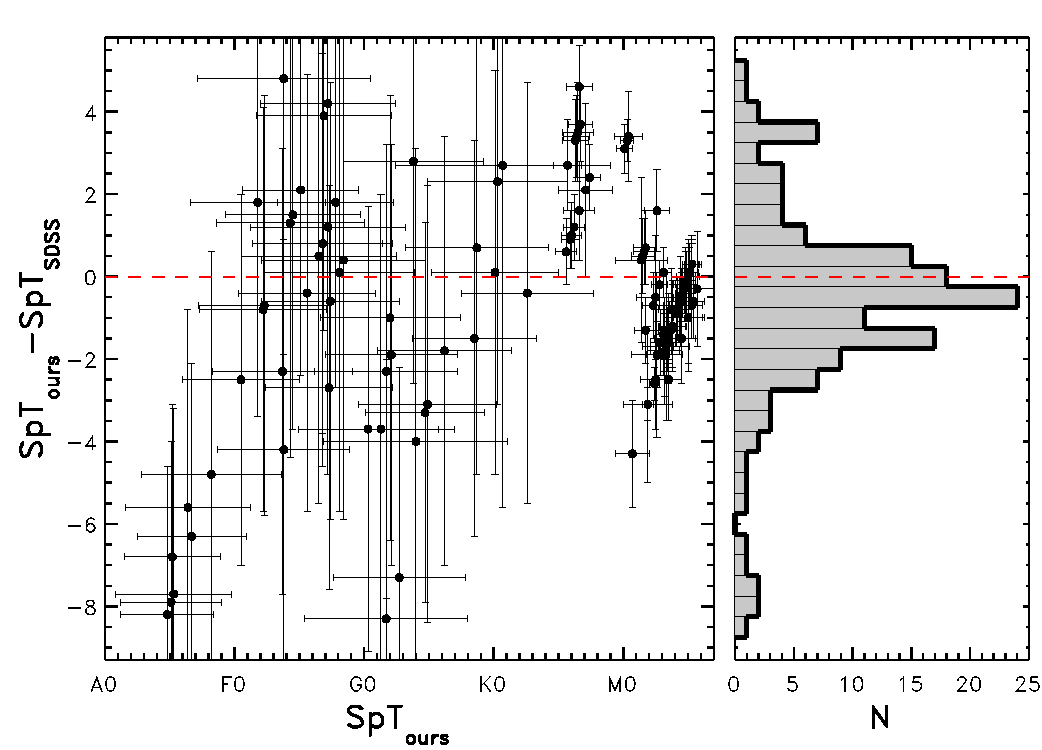
\includegraphics[width=1\textwidth]{f4.pdf}
	\end{minipage} \hfill
	\begin{minipage}{0.35\textwidth}
		\caption[SpT residuals between our classification and that from SDSS]{Residuals between our spectral type classification using the SPTCLASS code \citep{Hernandez2004} and the spectral type assigned by the SDSS pipeline. The associated errors are those estimated by the SPTCLASS code because the SDSS classification does not report spectral type uncertainties. The residuals are given in units of spectral sub-classes.}
		\label{fig_BOSS:sptclass}
	\end{minipage}
\end{figure}

\subsubsubsection{Membership Determination for 25 Ori and Orion OB1a}
\label{sec_BOSS:memberships}

Once the spectral type was determined for all the stars on the 25 Ori BOSS plate, several diagnoses were applied to determine their memberships, depending on their spectral types.

\paragraph{M-type Stars\\}
\label{sec_BOSS:M_stars}

The following criteria were used to assign the 25 Ori and Orion OB1a memberships of the M-type stars:

\begin{itemize}
	\item H$_\alpha$ emission.
				
		The detection of strong H$_\alpha$ emission in young LMSs is due to both the chromospheric activity and accretion phenomena that produce narrow symmetric and broader asymmetric H$_\alpha$ line profiles \citep{Muzerolle2005}, respectively. We considered as possible M-type members those stars showing H$_\alpha$ emission. However, because at the age of 25 Ori most of the accreting circumstellar disks have dissipated \citep{Calvet2005}, not only those sources having strong emissions related to accretion are necessary members. Thus, additional criteria are needed to support the memberships of those objects showing weak H$_\alpha$ emission.

	\item LiI$\lambda$6708 absorption.

		For LMSs, the LiI$\lambda$6708 absorption is a well-known indicator of youth \citep{Strom1989, Briceno1998}. It is present in the stellar surface of LMSs because they are fully convective in the PMS phase and the mixing timescale is shorter than the time they need to reach the MS \citep{Soderblom1993}. Therefore, we used the presence of the LiI$\lambda$6708 absorption as an additional membership criterion for the LMSs.

	\item Weak NaI$\lambda\lambda$8183, 8195 doublet in absorption relative to a field star of the same spectral type.

		An additional youth indicator for the M-type stars is the NaI$\lambda\lambda$8183,8195 doublet in absorption, which is sensitive to surface gravity. Since the PMS stars are still contracting, they have lower surface gravity than MS stars with the same spectral type, such that the NaI$\lambda\lambda$8183, 8195 doublet is measurably weaker in PMS sources \citep{Luhman2003a}. We compared the BOSS M-type spectra with templates for young and old field stars with the same spectral type from, respectively, \citet{Luhman2000}, \citet{Briceno2002}, \citet{Luhman2003b} and \citet{Luhman2004}, and \citet{Kirkpatrick1999}, to determine if the NaI$\lambda\lambda$8183,8195 doublet is consistent with the weak absorption expected for a bona fide young star.

\end{itemize}

Summarizing these criteria, we confirm a M-type star as a 25 Ori or Orion OB1a member if it exhibits any level of H$_\alpha$ emission and either LiI$\lambda$6708 absorption or NaI$\lambda\lambda$8183, 8195 absorption whose profile agrees with a young stellar template of the same spectral type. Based on these criteria, we confirmed a total of 53 members of 25 Ori or Orion OB1a with spectral types from M0 to M6. Three of these members (148, 153, and 156) have already been confirmed as young members by \citet{Downes2014}, so we can report the finding of a total of 50 new confirmed members of 25 Ori or Orion OB1a. In Table \ref{tab_BOSS:membership} we summarize the membership criteria for these confirmed members. About 87\% of the M-type confirmed members have LiI$\lambda$6708 absorption equivalent widths W(LiI)$>$0.15 \AA\ and the rest have a clear weak NaI$\lambda\lambda$8183, 8195 doublet. The 81\% of the members have the NaI$\lambda\lambda$8183, 8195 doublet in absorption consistent with the young stellar templates and for most of the remaining members the NaI$\lambda\lambda$8183, 8195 is not conclusive but they show a clear LiI$\lambda$6708 absorption. As an example, in Figure \ref{fig_BOSS:membership} we show the spectrum of the member 157 with enlargements of the H$_\alpha$ emission, LiI$\lambda$6708 absorption and weak NaI$\lambda\lambda$8183, 8195 absorption youth indicators we used to assign its membership.

The 50 new confirmed members represent an increase of $\approx 30\%$ the number of known sub-solar members of 25 Ori or Orion OB1a in the region covered by the considered BOSS plate \citep{Briceno2005,Briceno2007,Hernandez2007b,Downes2014,Downes2015}. Of these members, 22 are inside the \citet{Briceno2005,Briceno2007} estimated area of 25 Ori (1$^\circ$ radius), which represents an increase of $\approx 14\%$ in the number of 25 Ori confirmed members in the sub-solar mass range. Throughout this study, we conservatively worked with the 25 Ori estimated radius of 1$^\circ$, which is greater than the 0.5$^\circ$ radius of the 25 Ori overdensity estimated by \citet{Downes2014}.

\paragraph{K-type Stars\\}
\label{sec_BOSS:K_stars}

The H$_\alpha$ emission and LiI$\lambda$6708 absorption membership criteria discussed in Section \ref{sec_BOSS:M_stars} also apply for the K-type stars. Therefore, K-type stars were selected as YSOs when presenting H$_\alpha$ emission and LiI$\lambda$6708 absorption. From the 20 K-type stars in the BOSS stellar spectra, we did not confirm any K-type member. None present both LiI$\lambda$6708 absorption and H$_\alpha$ emission (only two stars have weak H$_\alpha$ emission, but those lack LiI$\lambda$6708 absorption).

\paragraph{Early-type Stars\\}
\label{sec_BOSS:early_stars}

The membership criteria discussed in Section \ref{sec_BOSS:M_stars} cannot be applied to stars earlier than K-type (43 stars of the sample). In fact, there is not a clear way to confirm these stars as young members with the available information. We checked the position of these stars in the $I$ vs $I-J$ color-magnitude diagram. We found that not a single early-type star lies within the 25 Ori locus, even when considering the effects of variability. The position of these stars is consistent with the field stars.

The most robust membership diagnostic for stars earlier than K spectral type is their kinematics, though X-ray emission, IR excesses or variability are useful secondary indicators. The spectral resolution of BOSS is not high enough to provide precise radial velocities to determine kinematic memberships for these early type stars, so we checked the other criteria. None of these stars have X-ray counterparts in the 3XMM-DR5 database \citep{Rosen2016} or in the Chandra Source Catalog \citep{Evans2010}. Additionally, none of these stars are high-probability variable stars according to the CVSO catalog or have IR excesses according to the photometric selection from \citet{Cottle2018}, based on 2MASS+WISE photometry and the algorithm developed by \citet{Koenig2014}. Therefore, the stars earlier than K spectral type on the 25 Ori BOSS plate are likely non-members.

\begin{table} \scriptsize
 \caption[Youth indicators of the confirmed members from the BOSS spectra]{Confirmed members and their youth indicators.}
 \label{tab_BOSS:membership}
 \begin{threeparttable}
  \setlength{\tabcolsep}{10pt}
  \renewcommand{\arraystretch}{1.034}
	\begin{minipage}{0.48\textwidth}
	  \begin{tabular}{ccccc}
		\toprule
		{\bf ID} & {\bf SpT} & {\bf WH$_\alpha$} & {\bf WLiI$\lambda6708$} & {\bf NaI} \\
		   &     & (\AA)       & (\AA)             &     \\
		\midrule
		66  & M0.3$\pm$0.5  & -2.062  & 0.4257  & 0   \\ 
	  	74  & M1.5$\pm$1.2  & -161.8  & 0.2514  & -1  \\ 
	  	79  & M1.9$\pm$0.4  & -247.7  & 0.3037  & 1   \\ 
	  	82  & M2.4$\pm$0.4  & -52.95  & 0.2569  & 1   \\ 
	  	89  & M2.8$\pm$0.6  & -5.843  & 0.1607  & 1   \\ 
	  	92  & M3.1$\pm$0.5  & -4.39   & ---     & 1   \\ 
	  	93  & M3.1$\pm$0.5  & -3.541  & 0.1659  & 1   \\ 
	  	96  & M3.2$\pm$0.5  & -4.448  & 0.3134  & 1   \\ 
	  	97  & M3.2$\pm$0.5  & -38.64  & 0.446   & 1   \\ 
	  	98  & M3.2$\pm$0.6  & -5.865  & 0.4586  & 1   \\ 
	  	107 & M3.5$\pm$0.5  & -39.31  & 0.2887  & 1   \\ 
	  	108 & M3.5$\pm$0.6  & -7.876  & ---     & 1   \\ 
	  	109 & M3.5$\pm$1.0  & -41.43  & 0.577   & 0   \\ 
	  	110 & M3.5$\pm$1.1  & -7.721  & 0.2379  & 1   \\ 
	  	111 & M3.7$\pm$0.6  & -4.347  & 0.4181  & 1   \\ 
	  	115 & M4.1$\pm$0.7  & -16.54  & 0.4601  & 1   \\ 
	  	116 & M4.1$\pm$0.7  & -6.188  & 0.4777  & 1   \\ 
	  	117 & M4.2$\pm$0.7  & -6.016  & 0.3093  & 1   \\ 
	  	118 & M4.3$\pm$0.7  & -9.375  & 0.412   & 1   \\ 
	  	119 & M4.4$\pm$1.1  & -14.06  & 0.3332  & -1  \\ 
	  	120 & M4.5$\pm$0.7  & -5.663  & ---     & 1   \\ 
	  	121 & M4.5$\pm$0.7  & -62.18  & 0.0799  & 1   \\ 
	  	123 & M4.5$\pm$0.6  & -6.398  & 0.5469  & 1   \\ 
	  	124 & M4.5$\pm$1.1  & -47.26  & 0.6343  & -1  \\ 
	  	125 & M4.6$\pm$0.6  & -7.454  & ---     & 1   \\ 
	  	126 & M4.6$\pm$0.6  & -8.915  & 0.3241  & 1   \\ 
	  	127 & M4.6$\pm$0.5  & -10.15  & 0.3781  & 0   \\ 
	  	128 & M4.6$\pm$0.5  & -3.17   & 0.5076  & 1   \\ 
		\bottomrule
	  \end{tabular}
	\end{minipage} \hfill
	\begin{minipage}{0.48\textwidth}
  	\setlength{\tabcolsep}{10pt}
	\renewcommand{\arraystretch}{1.0}
	  \begin{tabular}{ccccc}
		\toprule
		{\bf ID} & {\bf SpT} & {\bf WH$_\alpha$} & {\bf WLiI$\lambda6708$} & {\bf NaI} \\
		   &     & (\AA)       & (\AA)             &     \\
		\midrule
	  	129 & M4.7$\pm$0.5  & -74.23  & 0.2364  & 1   \\ 
	  	130 & M4.7$\pm$0.5  & -6.109  & 0.5821  & 1   \\ 
	  	131 & M4.7$\pm$0.5  & -4.569  & 0.5341  & 1   \\ 
	  	132 & M4.7$\pm$0.4  & -12.02  & 0.5568  & 1   \\ 
	  	133 & M4.7$\pm$0.5  & -12.18  & 0.3165  & 1   \\ 
	  	134 & M4.8$\pm$0.4  & -21.34  & 0.1725  & 1   \\ 
	  	135 & M4.8$\pm$0.5  & -59.07  & 0.4103  & 1   \\ 
	  	137 & M4.8$\pm$0.5  & -10.11  & 0.5883  & 1   \\ 
	  	139 & M4.8$\pm$0.9  & -14.6   & ---     & 1   \\ 
	  	141 & M5.0$\pm$0.6  & -9.543  & 0.5009  & 1   \\ 
	  	143 & M5.0$\pm$1.3  & -14.41  & 0.8292  & -1  \\ 
	  	144 & M5.0$\pm$1.1  & -14.36  & 0.8965  & 1   \\ 
	  	146 & M5.1$\pm$0.6  & -15.92  & 0.7128  & 1   \\ 
	  	147 & M5.1$\pm$0.6  & -12.69  & 0.6626  & 1   \\ 
	  	148 & M5.1$\pm$0.7  & -8.659  & 0.6687  & 1   \\ 
	  	149 & M5.1$\pm$0.7  & -11.33  & 0.593   & 1   \\ 
	  	150 & M5.3$\pm$0.6  & -13.43  & 0.354   & 0   \\ 
	  	151 & M5.3$\pm$0.5  & -14.57  & 0.3275  & 1   \\ 
	  	152 & M5.3$\pm$0.7  & -88.18  & 0.5188  & 1   \\ 
	  	153 & M5.3$\pm$0.6  & -32.65  & 0.534   & 1   \\ 
	  	154 & M5.3$\pm$0.6  & -12.34  & 0.7089  & 1   \\ 
	  	155 & M5.3$\pm$0.7  & -14.95  & 1.056   & 0   \\ 
	  	156 & M5.3$\pm$0.8  & -12.88  & ---     & 1   \\ 
	  	157 & M5.4$\pm$0.9  & -7.491  & 0.6515  & 1   \\ 
	  	158 & M5.7$\pm$1.4  & -29.84  & 1.712   & 0   \\ 
		\bottomrule
	  \end{tabular}
	  \begin{tablenotes}[para,flushleft]
	    For the NaI$\lambda\lambda$8183, 8195 absorption, the 1, -1, and 0 flags mean, respectively, if the feature is consistent with a young stellar template, an old stellar template or not conclusive.\\
	  \end{tablenotes}
	\end{minipage}
 \end{threeparttable}
\end{table}

\begin{figure*}[ht!]%[H]
	\centering 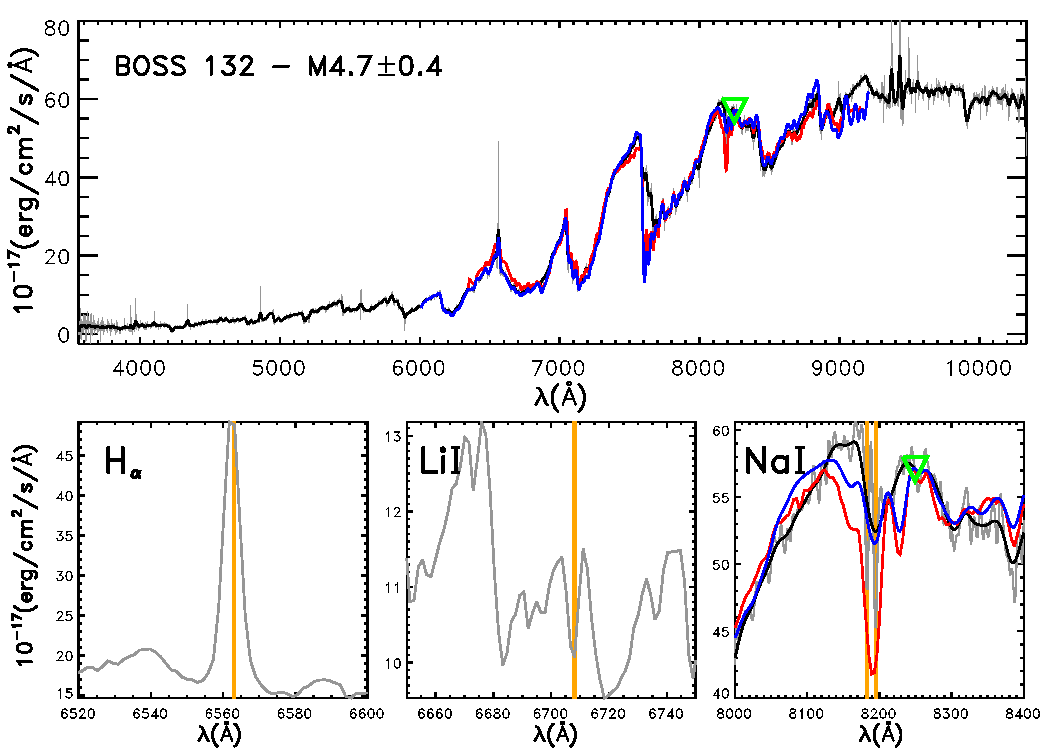
\includegraphics[width=1.\textwidth]{f5.pdf}
	\caption[Membership criteria for M-type stars]{Example of one of the confirmed LMS members in Orion OB1a (member 132 from Table \ref{tab_BOSS:membership}). \textbf {Upper panel:} BOSS spectrum with the original resolution of 1.4 \AA\ (gray solid line) and with a convolved resolution of 16 \AA\ (black solid line). The stellar templates with the same spectral type as this confirmed member are shown with a resolution of 16 \AA\ for a field star from \citet{Kirkpatrick1999} (red line) and for a young star from the lists by \citet{Luhman2000,Briceno2002,Luhman2003b} and \citet{Luhman2004} (blue line). The green triangle indicates the normalization point of the stellar templates' fluxes, which is located in the pseudo-continuum of the NaI$\lambda\lambda$8183, 8195 doublet of the BOSS spectrum \citep{Schlieder2012}. \textbf {Lower panel:} Enlargements of the H$_\alpha$ emission, LiI$\lambda$6708 absorption and weak NaI$\lambda\lambda$8183, 8195 doublet youth indicators used to assign the memberships of the LMSs. The orange vertical solid lines show the wavelength range of the indicated features. For member 132, the spectrum presents H$_\alpha$ emission, LiI$\lambda$6708 absorption and the NaI$\lambda\lambda$8183, 8195 doublet consistent with the young stellar template. Therefore, this star was confirmed as a young LMS member.}
	\label{fig_BOSS:membership}
\end{figure*}

\subsubsubsection{Physical Parameters}
\label{sec_BOSS:parameters}

As described in \citet{Luhman1999}, the $I$ and $J$ bands are preferred to estimate bolometric luminosities of young LMSs because the contamination from UV and IR excess emission is minimal. We used the $I$ band from the CDSO and the $J$ band from VISTA to determine the extinction and bolometric luminosity of our confirmed members.

\paragraph{Extinctions\\}
\label{sec_BOSS:extinction}
The visual extinction ($A_V$) toward each confirmed member was calculated using the observed $I-J$ color, an assumed intrinsic $I-J$ color for a young star of the same measured spectral type and the extinction law from \citet{Fitzpatrick1999}, assuming $R_V=3.1$. The adopted intrinsic $I-J$ color was obtained by interpolating the spectral type in the empirical relations from \citet{Kenyon-Hartmann1995}, \citet{Luhman1999}, \citet{Briceno2002}, and \citet{Luhman2003a}. These relationships were designed to match the \citet{Baraffe1998} tracks, as explained by \citet{Luhman2003b}.

In Table \ref{tab_BOSS:parameters} we list the extinctions we estimated toward each confirmed LMS member of 25 Ori or Orion OB1a. Removing the two members having the highest unexpected extinctions (member 74 and 109 with $A_V=4.33^{+0.51}_{-0.98}$ and $A_V=3.53^{+0.94}_{-1.01.}$ mag, respectively), we obtained a mean extinction $\bar{A_V}$=0.14 mag and a standard deviation $\sigma _{A_V}=0.31$ mag toward the complete sample of confirmed members in 25 Ori and Orion OB1a, which is agreement with the mean extinction $\bar{A_V}$=0.16 mag, obtained by \citet{Downes2015}. If we only consider the confirmed members inside the 25 Ori's estimated area, we obtain $\bar{A_V}$=0.21 mag and $\sigma _{A_V}=0.43$ mag, which is also in agreement with previous extinction estimates in 25 Ori \citep[0.27 mag, 0.28 mag, 0.29 mag, and 0.30 mag by ][respectively]{Kharchenko2005, Briceno2005, Briceno2007, Downes2014}.

\begin{table} \scriptsize
 \caption[Physical parameters of the confirmed members using BOSS spectra]{Physical parameters of the 53 confirmed members.}
 \label{tab_BOSS:parameters}
 \begin{threeparttable}
  	\setlength{\tabcolsep}{5pt}
	\begin{tabular}{lclclclclclccc}
	\toprule
	{\bf ID} & {\bf $A_\textrm{v}$} & {\bf e\_$A_\textrm{v}$} &  {\bf T$_{eff}$}   & {\bf e\_T$_{eff}$}  & {\bf L}           & {\bf e\_L}          & {\bf $m$}         & {\bf e\_$m$}        & {\bf age}   & {\bf e\_age} & {\bf TTS} & {\bf Disk Type} & {\bf Location} \\
	   & (mag.)         & (mag.)          & (K)  & (K) & (L$_\odot$) & (L$_\odot$) & (M$_\odot$) & (M$_\odot$) & (Myr) & (Myr)              &     &           & \\
	\midrule
 	66$^a  $    & 0.193 & $^{+0.325}_{-0.203}$ & 3806.5 & $^{+85.5  }_{-72.5 }$ & 0.286 & $^{+0.125 }_{-0.118}$ & 0.573 & $^{+0.038 }_{-0.073}$ & 4.175  & $^{+10.597 }_{-2.387}$  & WTTS & ClassIII & ASCC18/ASCC20 \\
 	74          & 4.33  & $^{+0.513}_{-0.975}$ & 3632.5 & $^{+174.0 }_{-174.0}$ & 0.312 & $^{+0.195 }_{-0.221}$ & 0.425 & $^{+0.101 }_{-0.125}$ & 2.026  & $^{+12.817 }_{-1.338}$  & CTTS & Evolved  & Outside       \\
 	79$^a  $    & 1.355 & $^{+0.183}_{-0.366}$ & 3574.5 & $^{+58.0  }_{-58.0 }$ & 0.111 & $^{+0.028 }_{-0.031}$ & 0.445 & $^{+0.036 }_{-0.045}$ & 8.959  & $^{+5.93   }_{-3.864}$  & CTTS & ClassII  & 25Ori         \\
 	82$^a  $    & 1.299 & $^{+0.426}_{-0.426}$ & 3502.0 & $^{+58.0  }_{-58.0 }$ & 0.276 & $^{+0.09  }_{-0.09 }$ & 0.353 & $^{+0.016 }_{-0.052}$ & 1.79   & $^{+1.686  }_{-0.853}$  & CTTS & ClassII  & 25Ori         \\
 	89$^a  $    & 0.147 & $^{+0.64 }_{-0.538}$ & 3444.0 & $^{+87.0  }_{-87.0 }$ & 0.126 & $^{+0.087 }_{-0.08 }$ & 0.331 & $^{+0.047 }_{-0.031}$ & 4.189  & $^{+10.642 }_{-2.699}$  & WTTS & ClassIII & 25Ori/ASCC18  \\
 	92          & 0.0   & $^{+0.508}_{-0.0  }$ & 3400.5 & $^{+72.5  }_{-72.5 }$ & 0.081 & $^{+0.036 }_{-0.029}$ & 0.306 & $^{+0.053 }_{-0.024}$ & 6.79   & $^{+8.043  }_{-3.529}$  & WTTS & ClassIII & ASCC20        \\
 	93$^a  $    & 0.0   & $^{+0.508}_{-0.0  }$ & 3400.5 & $^{+72.5  }_{-72.5 }$ & 0.117 & $^{+0.074 }_{-0.061}$ & 0.3   & $^{+0.047 }_{-0.019}$ & 3.808  & $^{+11.07  }_{-2.231}$  & WTTS & ClassIII & ASCC18/ASCC20 \\
 	96$^a  $    & 0.33  & $^{+0.482}_{-0.406}$ & 3386.0 & $^{+72.5  }_{-72.5 }$ & 0.119 & $^{+0.052 }_{-0.049}$ & 0.299 & $^{+0.035 }_{-0.034}$ & 3.704  & $^{+7.801  }_{-1.933}$  & WTTS & ClassIII & ASCC20        \\
 	97$^a  $    & 1.168 & $^{+0.482}_{-0.406}$ & 3386.0 & $^{+72.5  }_{-72.5 }$ & 0.139 & $^{+0.062 }_{-0.058}$ & 0.296 & $^{+0.034 }_{-0.031}$ & 2.977  & $^{+6.142  }_{-1.566}$  & CTTS & TDC      & ASCC18        \\
 	98$^a  $    & 0.386 & $^{+0.589}_{-0.487}$ & 3386.0 & $^{+87.0  }_{-87.0 }$ & 0.13  & $^{+0.077 }_{-0.073}$ & 0.297 & $^{+0.047 }_{-0.051}$ & 3.271  & $^{+11.597 }_{-1.978}$  & WTTS & ClassIII & Outside       \\
 	107$^a $    & 0.33  & $^{+0.406}_{-0.406}$ & 3342.5 & $^{+72.5  }_{-72.5 }$ & 0.156 & $^{+0.082 }_{-0.082}$ & 0.272 & $^{+0.028 }_{-0.058}$ & 2.208  & $^{+6.233  }_{-1.237}$  & CTTS & Evolved  & Outside       \\
 	108         & 0.0   & $^{+0.513}_{-0.0  }$ & 3342.5 & $^{+87.0  }_{-87.0 }$ & 0.113 & $^{+0.066 }_{-0.06 }$ & 0.278 & $^{+0.025 }_{-0.076}$ & 3.513  & $^{+11.273 }_{-2.028}$  & WTTS & ClassIII & Outside       \\
 	109         & 3.533 & $^{+0.939}_{-1.066}$ & 3342.5 & $^{+145.0 }_{-145.0}$ & 0.157 & $^{+0.118 }_{-0.118}$ & 0.271 & $^{+0.075 }_{-0.071}$ & 2.188  & $^{+12.64  }_{-1.683}$  & CTTS & ClassII  & 25Ori         \\
 	110         & 0.0   & $^{+1.046}_{-0.0  }$ & 3342.5 & $^{+159.5 }_{-159.5}$ & 0.096 & $^{+0.086 }_{-0.069}$ & 0.282 & $^{+0.088 }_{-0.084}$ & 4.537  & $^{+10.338 }_{-3.771}$  & WTTS & ClassIII & Outside       \\
 	111         & 0.0   & $^{+0.487}_{-0.0  }$ & 3313.5 & $^{+87.0  }_{-87.0 }$ & 0.093 & $^{+0.046 }_{-0.04 }$ & 0.263 & $^{+0.037 }_{-0.063}$ & 4.353  & $^{+8.988  }_{-2.617}$  & WTTS & ClassIII & ASCC20        \\
 	115$^a $    & 0.046 & $^{+0.62 }_{-0.924}$ & 3255.5 & $^{+101.5 }_{-101.5}$ & 0.042 & $^{+0.027 }_{-0.029}$ & 0.207 & $^{+0.088 }_{-0.028}$ & 8.578  & $^{+6.298  }_{-5.968}$  & CTTS & TDC      & Outside       \\
 	116         & 0.0   & $^{+0.619}_{-0.0  }$ & 3255.5 & $^{+101.5 }_{-101.5}$ & 0.13  & $^{+0.083 }_{-0.074}$ & 0.218 & $^{+0.054 }_{-0.039}$ & 2.19   & $^{+8.071  }_{-1.685}$  & WTTS & Evolved  & Outside       \\
 	117         & 0.0   & $^{+0.67 }_{-0.0  }$ & 3241.0 & $^{+101.5 }_{-101.5}$ & 0.122 & $^{+0.07  }_{-0.058}$ & 0.206 & $^{+0.062 }_{-0.04 }$ & 2.204  & $^{+5.67   }_{-1.606}$  & WTTS & TDC      & ASCC20        \\
 	118$^a $    & 0.162 & $^{+0.721}_{-0.924}$ & 3226.5 & $^{+101.5 }_{-101.5}$ & 0.076 & $^{+0.044 }_{-0.047}$ & 0.2   & $^{+0.07  }_{-0.049}$ & 3.528  & $^{+11.281 }_{-2.451}$  & WTTS & Evolved  & ASCC20        \\
 	119         & 0.188 & $^{+1.097}_{-1.401}$ & 3212.0 & $^{+159.5 }_{-154.5}$ & 0.029 & $^{+0.028 }_{-0.03 }$ & 0.185 & $^{+0.115 }_{-0.085}$ & 10.461 & $^{+---    }_{-8.376}$  & WTTS & ClassIII & Outside       \\
 	120         & 0.0   & $^{+0.822}_{-0.0  }$ & 3197.5 & $^{+101.5 }_{-99.5 }$ & 0.052 & $^{+0.032 }_{-0.026}$ & 0.192 & $^{+0.058 }_{-0.067}$ & 4.924  & $^{+9.879  }_{-3.435}$  & WTTS & TDC      & ASCC20        \\
 	121$^a $    & 0.391 & $^{+0.823}_{-0.904}$ & 3197.5 & $^{+101.5 }_{-99.5 }$ & 0.021 & $^{+0.013 }_{-0.014}$ & 0.173 & $^{+0.067 }_{-0.048}$ & 14.128 & $^{+0.742  }_{-9.579}$  & CTTS & ClassII  & ASCC20        \\
 	123$^a $    & 0.0   & $^{+0.741}_{-0.0  }$ & 3197.5 & $^{+87.0  }_{-86.0 }$ & 0.068 & $^{+0.038 }_{-0.03 }$ & 0.198 & $^{+0.042 }_{-0.06 }$ & 3.635  & $^{+7.512  }_{-2.437}$  & WTTS & ClassII  & ASCC18        \\
 	124         & 0.0   & $^{+1.147}_{-0.0  }$ & 3197.5 & $^{+159.5 }_{-153.5}$ & 0.049 & $^{+0.044 }_{-0.037}$ & 0.191 & $^{+0.099 }_{-0.091}$ & 5.272  & $^{+9.602  }_{-4.006}$  & CTTS & Evolved  & 25Ori         \\
 	125         & 0.0   & $^{+0.792}_{-0.0  }$ & 3183.0 & $^{+87.0  }_{-85.0 }$ & 0.079 & $^{+0.045 }_{-0.036}$ & 0.192 & $^{+0.038 }_{-0.066}$ & 2.755  & $^{+6.192  }_{-1.742}$  & WTTS & TDC      & ASCC20        \\
 	126         & 0.0   & $^{+0.792}_{-0.0  }$ & 3183.0 & $^{+87.0  }_{-85.0 }$ & 0.042 & $^{+0.024 }_{-0.019}$ & 0.182 & $^{+0.042 }_{-0.056}$ & 5.805  & $^{+8.994  }_{-3.891}$  & WTTS & TDC      & ASCC20        \\
 	127$^a $    & 0.0   & $^{+0.66 }_{-0.0  }$ & 3183.0 & $^{+72.5  }_{-71.5 }$ & 0.14  & $^{+0.069 }_{-0.056}$ & 0.183 & $^{+0.039 }_{-0.045}$ & 1.118  & $^{+2.595  }_{-0.612}$  & WTTS & ClassIII & ASCC18        \\
 	128         & 0.0   & $^{+0.66 }_{-0.0  }$ & 3183.0 & $^{+72.5  }_{-71.5 }$ & 0.025 & $^{+0.014 }_{-0.013}$ & 0.171 & $^{+0.036 }_{-0.033}$ & 10.55  & $^{+4.332  }_{-6.362}$  & WTTS & ClassII  & Outside       \\
 	129$^a $    & 0.619 & $^{+0.66 }_{-0.64 }$ & 3168.5 & $^{+72.5  }_{-70.5 }$ & 0.09  & $^{+0.044 }_{-0.044}$ & 0.178 & $^{+0.028 }_{-0.053}$ & 1.966  & $^{+5.167  }_{-1.028}$  & CTTS & Evolved  & ASCC20        \\
 	130$^a $    & 0.0   & $^{+0.66 }_{-0.0  }$ & 3168.5 & $^{+72.5  }_{-70.5 }$ & 0.052 & $^{+0.026 }_{-0.021}$ & 0.18  & $^{+0.021 }_{-0.055}$ & 4.194  & $^{+7.27   }_{-2.586}$  & WTTS & TDC      & ASCC18        \\
 	131         & 0.0   & $^{+0.66 }_{-0.0  }$ & 3168.5 & $^{+72.5  }_{-70.5 }$ & 0.08  & $^{+0.04  }_{-0.033}$ & 0.18  & $^{+0.026 }_{-0.055}$ & 2.371  & $^{+4.579  }_{-1.325}$  & WTTS & ClassIII & ASCC18        \\
 	132$^a $    & 0.0   & $^{+0.528}_{-0.0  }$ & 3168.5 & $^{+58.0  }_{-57.0 }$ & 0.215 & $^{+0.112 }_{-0.1  }$ & 0.181 & $^{+0.019 }_{-0.043}$ & 0.623  & $^{+1.55   }_{-0.116}$  & WTTS & TDC      & Outside       \\
 	133         & 0.0   & $^{+0.66 }_{-0.0  }$ & 3168.5 & $^{+72.5  }_{-70.5 }$ & 0.087 & $^{+0.05  }_{-0.044}$ & 0.179 & $^{+0.028 }_{-0.053}$ & 2.075  & $^{+5.654  }_{-1.17 }$  & WTTS & ClassIII & Outside       \\
 	134         & 0.0   & $^{+0.528}_{-0.0  }$ & 3154.0 & $^{+58.0  }_{-56.0 }$ & 0.03  & $^{+0.013 }_{-0.011}$ & 0.163 & $^{+0.031 }_{-0.037}$ & 7.27   & $^{+7.53   }_{-4.032}$  & CTTS & TDC      & ASCC20        \\
 	135         & 0.0   & $^{+0.66 }_{-0.0  }$ & 3154.0 & $^{+72.5  }_{-69.5 }$ & 0.061 & $^{+0.044 }_{-0.036}$ & 0.173 & $^{+0.027 }_{-0.058}$ & 3.113  & $^{+10.263 }_{-1.943}$  & CTTS & Evolved  & ASCC18/ASCC20 \\
 	137         & 0.0   & $^{+0.66 }_{-0.0  }$ & 3154.0 & $^{+72.5  }_{-69.5 }$ & 0.06  & $^{+0.035 }_{-0.031}$ & 0.173 & $^{+0.027 }_{-0.058}$ & 3.222  & $^{+8.17   }_{-1.924}$  & WTTS & TDC      & Outside       \\
 	139         & 0.005 & $^{+1.137}_{-1.117}$ & 3154.0 & $^{+130.5 }_{-123.5}$ & 0.03  & $^{+0.026 }_{-0.026}$ & 0.163 & $^{+0.071 }_{-0.064}$ & 7.27   & $^{+7.593  }_{-5.211}$  & WTTS & TDC      & Outside       \\
 	141         & 0.0   & $^{+0.792}_{-0.0  }$ & 3125.0 & $^{+87.0  }_{-81.0 }$ & 0.037 & $^{+0.022 }_{-0.019}$ & 0.152 & $^{+0.048 }_{-0.052}$ & 4.762  & $^{+10.03  }_{-2.779}$  & WTTS & TDC      & ASCC18        \\
 	143         & 0.112 & $^{+1.564}_{-1.873}$ & 3125.0 & $^{+188.5 }_{-168.0}$ & 0.027 & $^{+0.035 }_{-0.037}$ & 0.149 & $^{+0.11  }_{-0.069}$ & 6.993  & $^{+---    }_{-5.394}$  & WTTS & ClassII  & Outside       \\
 	144         & 0.33  & $^{+1.401}_{-1.437}$ & 3125.0 & $^{+159.5 }_{-146.0}$ & 0.026 & $^{+0.029 }_{-0.029}$ & 0.148 & $^{+0.086 }_{-0.066}$ & 7.309  & $^{+---    }_{-5.331}$  & WTTS & ClassII  & Outside       \\
 	146         & 0.0   & $^{+0.782}_{-0.0  }$ & 3111.5 & $^{+86.0  }_{-81.0 }$ & 0.021 & $^{+0.018 }_{-0.016}$ & 0.139 & $^{+0.048 }_{-0.04 }$ & 8.428  & $^{+6.447  }_{-5.537}$  & WTTS & TDC      & 25Ori/ASCC20  \\
 	147         & 0.0   & $^{+0.782}_{-0.0  }$ & 3111.5 & $^{+86.0  }_{-81.0 }$ & 0.041 & $^{+0.034 }_{-0.029}$ & 0.146 & $^{+0.054 }_{-0.047}$ & 3.998  & $^{+10.89  }_{-2.444}$  & WTTS & Evolved  & 25Ori/ASCC18  \\
 	148         & 0.0   & $^{+0.914}_{-0.0  }$ & 3111.5 & $^{+100.5 }_{-94.5 }$ & 0.039 & $^{+0.026 }_{-0.022}$ & 0.146 & $^{+0.054 }_{-0.056}$ & 4.187  & $^{+10.589 }_{-2.437}$  & WTTS & Evolved  & 25Ori         \\
 	149         & 0.0   & $^{+0.914}_{-0.0  }$ & 3111.5 & $^{+100.5 }_{-94.5 }$ & 0.075 & $^{+0.056 }_{-0.049}$ & 0.145 & $^{+0.055 }_{-0.045}$ & 1.714  & $^{+10.208 }_{-1.208}$  & WTTS & ClassIII & Outside       \\
 	150         & 0.0   & $^{+0.761}_{-0.0  }$ & 3084.5 & $^{+84.0  }_{-81.0 }$ & 0.195 & $^{+0.12  }_{-0.103}$ & 0.162 & $^{+0.031 }_{-0.066}$ & 0.506  & $^{+1.392  }_{----  }$  & WTTS & ClassIII & ASCC20        \\
 	151         & 0.0   & $^{+0.63 }_{-0.0  }$ & 3084.5 & $^{+69.5  }_{-67.5 }$ & 0.136 & $^{+0.072 }_{-0.063}$ & 0.15  & $^{+0.027 }_{-0.056}$ & 0.842  & $^{+1.545  }_{-0.334}$  & WTTS & ClassIII & ASCC20        \\
 	152         & 0.0   & $^{+0.894}_{-0.0  }$ & 3084.5 & $^{+98.5  }_{-94.5 }$ & 0.027 & $^{+0.019 }_{-0.016}$ & 0.127 & $^{+0.057 }_{-0.036}$ & 5.486  & $^{+9.401  }_{-3.097}$  & CTTS & ClassII  & 25Ori         \\
 	153         & 0.0   & $^{+0.762}_{-0.0  }$ & 3084.5 & $^{+84.0  }_{-81.0 }$ & 0.047 & $^{+0.028 }_{-0.024}$ & 0.128 & $^{+0.053 }_{-0.032}$ & 2.666  & $^{+8.041  }_{-1.183}$  & CTTS & Evolved  & 25Ori         \\
 	154         & 0.0   & $^{+0.762}_{-0.0  }$ & 3084.5 & $^{+84.0  }_{-81.0 }$ & 0.057 & $^{+0.036 }_{-0.031}$ & 0.132 & $^{+0.046 }_{-0.036}$ & 2.18   & $^{+7.117  }_{-1.253}$  & WTTS & TDC      & ASCC18        \\
 	155         & 0.0   & $^{+0.894}_{-0.0  }$ & 3084.5 & $^{+98.5  }_{-94.5 }$ & 0.014 & $^{+0.01  }_{-0.008}$ & 0.119 & $^{+0.051 }_{-0.027}$ & 11.845 & $^{+3.031  }_{-7.036}$  & WTTS & ClassIII & 25Ori         \\
 	156$^a $    & 0.0   & $^{+1.025}_{-0.0  }$ & 3084.5 & $^{+113.0 }_{-105.5}$ & 0.038 & $^{+0.03  }_{-0.025}$ & 0.127 & $^{+0.072 }_{-0.046}$ & 3.463  & $^{+11.422 }_{-1.926}$  & WTTS & ClassII  & 25Ori         \\
 	157         & 0.0   & $^{+1.148}_{-0.0  }$ & 3071.0 & $^{+126.5 }_{-114.0}$ & 0.026 & $^{+0.026 }_{-0.021}$ & 0.12  & $^{+0.072 }_{-0.042}$ & 5.335  & $^{+9.537  }_{-3.422}$  & WTTS & TDC      & Outside       \\
 	158         & 0.0   & $^{+1.777}_{-0.0  }$ & 3030.5 & $^{+196.0 }_{-167.5}$ & 0.019 & $^{+0.032 }_{-0.023}$ & 0.098 & $^{+0.102 }_{-0.026}$ & 6.334  & $^{+---    }_{-5.676}$  & CTTS & ClassII  & Outside       \\
	\bottomrule
	\end{tabular}
	\begin{tablenotes}[para,flushleft]
	  {\bf Note}. Outside location label indicates the members not belonging to any stellar group defined by \citet{Kharchenko2013}.\\
      $^a$ $>99\%$ probable variable star according to the CVSO study.\\
	\end{tablenotes}
 \end{threeparttable}
\end{table}

\paragraph{Effective Temperatures and Bolometric Luminosities\\}
\label{sec_BOSS:HR}

We estimated the effective temperatures of the confirmed members by interpolating their spectral types into the empirical relations from \citet{Luhman1999}.

To compute the bolometric luminosities of these members, we used newly available Gaia data \citep[\ac{Gaia DR1}; ][]{GaiaCollaboration2016} to establish distances for the 25 Ori, ASCC 18, and ASCC 20 stellar groups, where the confirmed members are located. In Table \ref{tab_BOSS:distances} we summarize the previous distances to these groups \citep{Kharchenko2005,Briceno2005,Briceno2007,Kharchenko2013,Downes2014}, as well as our own estimates from the Gaia DR1 parallaxes for the higher probability \citet{Kharchenko2005} members of these groups. The Gaia-based distance estimates for the 25 Ori, ASCC 18, and ASCC 20 stellar groups are, within the uncertainties, essentially identical of 338$\pm$66 pc. We then used individual distance estimates derived from Gaia DR1 parallaxes to calculate the absolute $I$ magnitudes (M$_\textrm{\scriptsize {I}}$) for the confirmed members projected inside these stellar groups. For members located outside these groups, we assumed the mean Gaia distance. Then we used the bolometric correction from \citet{Kenyon-Hartmann1995} to obtain the bolometric luminosity, assuming M$_{\textrm{\scriptsize{bol}}_\odot}=4.755$ \citep{Mamajek2012}. In Figure \ref{fig_BOSS:H-R} we show the locations of the confirmed members in the H-R diagrams according to the stellar group where they lie or if they are outside of the groups indicated in Figure \ref{fig_BOSS:sky} and in Table \ref{tab_BOSS:parameters} are listed the effective temperatures and bolometric luminosities we estimated for the confirmed members.

\begin{table} \scriptsize
\begin{center}
 \caption[Distances for the clusters where lie the confirmed members from the BOSS spectra]{Distances of the stellar groups partially covered by the 25 Ori BOSS plate.}
 \label{tab_BOSS:distances}
 \begin{threeparttable}
  	\setlength{\tabcolsep}{15pt}
	\begin{tabular}{lccc}
	\toprule
	{\bf Reference} & \multicolumn{3}{c}{{\bf Distance}} \\
		            & \multicolumn{3}{c}{(pc)} \\
	\cline{2-4}
 	            & {\bf 25 Ori} & {\bf ASCC 18} & {\bf ASCC 20} \\
	\midrule
	\citet{Kharchenko2005}          & 460            & 500            & 450 \\
	\citet{Kharchenko2013}          & 397            & 313            & 394 \\
	\citet{Briceno2005,Briceno2007} & 330            & ...            & ... \\
	\citet{Downes2014}              & 360            & ...            & ... \\
	\citet{GaiaCollaboration2016}   & 336$\pm$30$^a$ & 349$\pm$44$^b$ & 330$\pm$39$^c$ \\
	\bottomrule
	\end{tabular}
	\begin{tablenotes}[para,flushleft]
	  $^a$ for 17 high-probability members.\\
	  $^b$ for 7 high-probability members.\\
	  $^c$ for 15 high-probability members.\\
	\end{tablenotes}
 \end{threeparttable}
\end{center}
\end{table}

\begin{figure*}[ht!]
	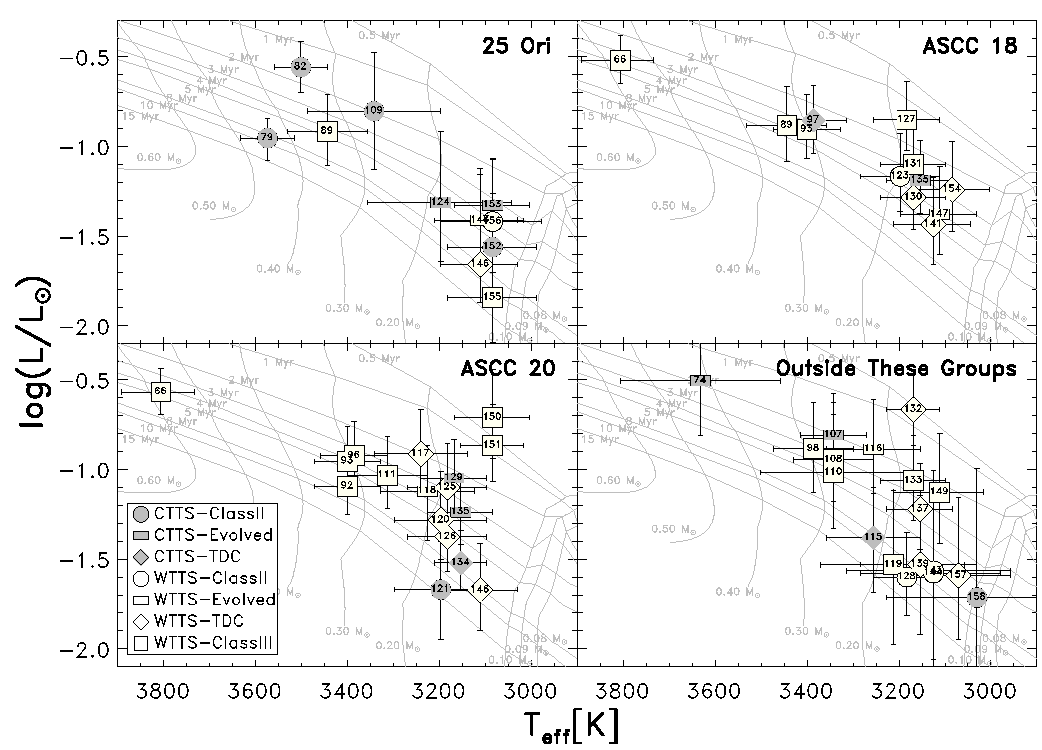
\includegraphics[width=1.\textwidth]{f6.pdf}
	\caption[H-R diagram of the confirmed members from the BOSS spectra]{H-R diagrams of the confirmed members inside the labeled stellar groups or outside them, according to \citet{Kharchenko2013}. The gray curves represent the PMS \citet{Baraffe2015} models. The members overlapping two of the stellar groups indicated in Figure \ref{fig_BOSS:sky} appear in both H-R diagrams.
	\label{fig_BOSS:H-R}}
\end{figure*}

\paragraph{Masses and Ages\\}

As shown in Figure \ref{fig_BOSS:H-R}, all members are scattered, within the uncertainties, throughout the 1-10 Myr isochrones and 0.1-0.6 M$_\odot$ evolutionary tracks, adopting the PMS models from \citet{Baraffe2015}.

To better estimate the masses and ages of the confirmed members, we interpolated their effective temperatures and bolometric luminosities into the \citet{Baraffe2015} models. When a confirmed member overlaps two stellar groups we adopted its mean bolometric luminosity. In Table \ref{tab_BOSS:parameters} we show the mass and age we obtained for each confirmed member. The resulting masses for the 53 confirmed members are in a range from 0.10 M$_\odot$ to 0.58 M$_\odot$, with $64\%$ of the members having masses lower than 0.20 M$_\odot$. This implies that in this mass range we increased by a $\approx50\%$ the number of confirmed LMSs in the region covered by the BOSS plate, and by a $\approx$20\% the number of LMSs in the estimated area of 25 Ori \citep[1$^\circ$ radius; ][]{Briceno2005,Briceno2007}.

The ages we calculated for the confirmed members are roughly twice younger than those found with similar methods in previous studies for the stellar groups where they are located \citep{Kharchenko2005,Briceno2005,Briceno2007,Kharchenko2013,Downes2014}. This is due to the target selection bias in the 25 Ori BOSS spectra (see Section \ref{sec_BOSS:spectroscopy} and Figure \ref{fig_BOSS:CCD_bias}).

For all the confirmed members we estimated the uncertainties in the derived values of the main physical parameters (extinction, effective temperature, bolometric luminosity, mass, and age) by considering the following factors: the error propagation that applies to each step described in this section and the errors associated to the interpolations. In Table \ref{tab_BOSS:parameters} we show the resulting uncertainties for the extinction, effective temperature, bolometric luminosity, mass, and age values for the confirmed members. We also indicate to which stellar group they belong.

\subsubsubsection{T Tauri Star Classification}
\label{sec_BOSS:TTSclass}

The BOSS low-resolution spectra allowed us to measure the H$_\alpha$ equivalent width, which we used, together with the spectral types, to classify the confirmed members as either accreting young LMSs (classical T Tauri stars; CTTSs) or non-accreting young LMSs (weak T Tauri stars; WTTSs). To define the limit between both types of T Tauri stars (TTSs), we adopted the empirical saturation criterion by \citet{BarradoYNavascues-Martin2003}, in which stars with H$_\alpha$ emission above this limit are classified as CTTSs, and otherwise as WTTSs. In Figure \ref{fig_BOSS:WHavsSpT} we show the TTS classification scheme and in Table \ref{tab_BOSS:parameters} we show the resulting classification for the whole sample of confirmed members.

We confirmed a total of 15 CTTSs and 38 WTTSs among the 53 members in the BOSS sample. This corresponds to a very high fraction of CTTSs to WTTSs compared to the values of 5.6\% and 3.8$\pm0.4$\% found by \citet{Briceno2007} and \citet{Downes2014}, respectively, which is due to the target selection bias toward sources with IR excesses.

\begin{figure}[ht!]
	\begin{minipage}{0.60\textwidth}
		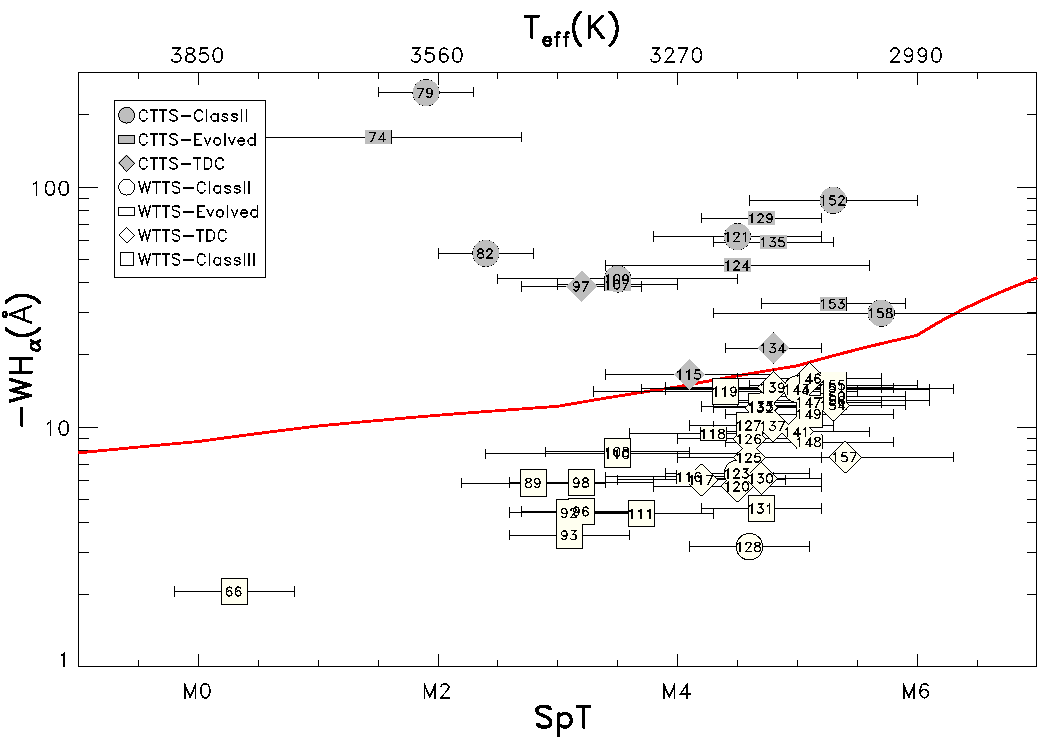
\includegraphics[width=1.0\textwidth]{f7.pdf}
	\end{minipage} \hfill
	\begin{minipage}{0.35\textwidth}
		\caption[TTS classification of the confirmed members from the BOSS spectra]{Relation between the H$_\alpha$ equivalent widths and spectral types for the confirmed members. The red solid curve indicates the saturation limit from \citet{BarradoYNavascues-Martin2003}, which allow us to separate WTTSs from CTTSs. The upper axis shows the effective temperature corresponding to the spectral types \citep{Luhman2003b}.}
		\label{fig_BOSS:WHavsSpT}
	\end{minipage}
\end{figure}

\subsubsubsection{Spectral Energy Distributions}
\label{sec_BOSS:SED}

The circumstellar disks of the YSOs were classified according to their IR excess emissions at $\lambda>2\ \mu$m. Objects having a flat or decreasing IR spectral energy distribution (\ac{SED}) are considered Class II, while Class III objects have little or no near-IR excess \citep{Lada-Wilking1984,Lada1987}. An intermediate phase between the Class II and Class III objects contains the so-called ``transitional disk systems" that present a decreasing SED slope in the near-IR that rises again in the mid-IR. Finally, the ``evolved disk systems" show a monotonically decreasing IR SED \citep[e.g.,][]{Hernandez2007b}.

To classify the IR excesses of the confirmed members according to this scheme, we constructed their SEDs using the Virtual Observatory SED Analyzer (\ac{VOSA}) tool \citep{Bayo2008} and the photometric catalogs described in Sections \ref{sec_BOSS:Optphot} and \ref{sec_BOSS:IRphot}, and listed in Table \ref{tab_BOSS:photometry}. We have a minimum of 10 and a maximum of 24 photometric bands for each confirmed member, covering a wavelength range from 0.36 $\mu$m to 22 $\mu$m.

The SEDs were dereddened using the visual extinction we estimated in Section \ref{sec_BOSS:extinction} and assuming the extinction law reported by \citet{Fitzpatrick1999} and subsequently improved by \citet{Indebetouw2005}. To determine the corresponding IR excesses we proceeded iteratively as follows: First, we fitted the SEDs to the PMS LMS models from \cite{Baraffe2015}, restricting the effective temperature range to the one obtained in Section \ref{sec_BOSS:HR}. During this iteration we only considered the photometric bands where the IR excesses are not expected to occur ($\lambda < 2\ \mu$m).

From the resulting fitted SEDs, VOSA automatically detects which bands present IR excesses by using an improved algorithm from that by \citet{Lada2006}, which measures the slope of the IR points in the log($\lambda F_\lambda$) vs log($\lambda$) space. Basically, when the slope becomes greater than -2.56, the IR excesses are determined.

Then, a second fit to the \cite{Baraffe2015} models was performed, this time excluding those photometric bands showing IR excesses. In this way, we avoided false IR excess detections during the first iteration and maximized the number of photometric bands used for fitting the photospheres. The number of photometric bands used during the second iteration ran from 10 to 23 (except for the members 74 and 109 with 7 and 8 fitted bands, respectively). In Figure \ref{fig_BOSS:SEDs} we show the resulting SEDs for a selection of the confirmed members. The bolometric luminosities for the confirmed members corresponding to the total flux of the best \citet{Baraffe2015} model fit are in agreement, within the uncertainties, with those obtained using the $I$ band, as explained in Section \ref{sec_BOSS:HR}.

\begin{figure*}[ht!]
	\centering
	\includegraphics[width=1.0\textwidth]{f8.pdf}
	\caption[SEDs of the confirmed members from the BOSS spectra]{Dereddened SEDs for a sample of the confirmed members (black points and black solid curves). The gray spectra correspond to the best PMS LMS model from \citet{Baraffe2015} fitted to the dereddened data bluer than the point were the IR excesses start (vertical black dashed line). The black dotted curves show the fitted \citet{Baraffe2015} model spectra in a lower resolution. The red dashed curves and the blue dotted ones indicate, respectively, the median SEDs of Class II disks of the $\sigma$ Orionis cluster \citep{Hernandez2007a} and the Taurus star-forming region \citep{Furlan2006}, normalized to the dereddened $J$-band flux of each member. The vertical red and blue solid lines represent the upper and lower quartiles for these median SEDs. Each SED has a label with the member ID and its TTS and disk classifications, as explained in Sections \ref{sec_BOSS:TTSclass} and \ref{sec_BOSS:SED}, respectively. The photometric errors are included but most of them are smaller than the corresponding symbols. All the SEDs of the confirmed members are available in the electronic version of the \citealt{Suarez2017} publication.}
	\label{fig_BOSS:SEDs}
\end{figure*}

We classified the members as Class II if their IR SEDs resemble the median SEDs of Class II disks of the $\sigma$ Orionis cluster \citep{Hernandez2007a} and the Taurus star-forming region \citep{Furlan2006}. The members showing lower IR excesses were considered evolved systems, while the members having IR SEDs consistent with the photospheric \citet{Baraffe2015} model fit were classified as Class III. The members showing a near-IR SED consistent with evolved systems or Class III objects, but having an unexpected strong excess at 22 $\mu$m were considered as transitional disk candidates (\ac{TDC}s).

For the 14 members having available photometry in the [3.6] and [8.0] bands from IRAC, the slope in the [3.6]-[8.0] color ($\alpha$, in the log[$\lambda F_\lambda$] vs log[$\lambda$] space) was analyzed to improve the disk classification as follows \citep{Lada2006}: Class II objects have slopes of $-1.8<\alpha<0$; evolved or ``anemic" disk systems \citep{Hernandez2007a} have $-2.56\le\alpha<-1.8$ slopes; Class III objects have $\alpha<-2.56$. In Figure \ref{fig_BOSS:irac} we show the locations of the members in the IRAC color-color diagrams. All the CTTSs fall inside the CTTS locus defined by \citet{Hartmann2005}, but four objects classified as WTTSs also fall inside this region (two having evolved disks, one is a TDC and the other one is bearing a Class II disk). All the members located in the IR excess region defined by \citet{Luhman2005} have Class II disks and only one of them has an evolved disk. The rest of the evolved systems and TDCs are located in the region between the Class II and Class III objects, as expected from the \citet{Hernandez2007b} sample. 

\begin{figure*}[ht!]
	\centering
	\includegraphics[width=1.0\textwidth]{f9.pdf}
	\caption[IRAC color-color diagrams of the confirmed members from the BOSS spectra]{IRAC color-color diagrams for the confirmed members from this work (top panels) and including those from \citet{Hernandez2007b} (bottom panels). The small black filled circles, diamonds, horizontal bars and square represent YSOs with Class II, transitional, evolved or Class III disks from \citet{Hernandez2007b}. The dashed lines delimit the region where M type objects with disk are expected, from the study by \citet{Luhman2005}, and the dotted lines show the CTTS locus from \citet{Hartmann2005}.}
	\label{fig_BOSS:irac}
\end{figure*}

Of the 53 confirmed members we classified: $a)$ 11 Class II objects, with SEDs consistent with the $\sigma$ Orionis cluster and Taurus star-forming region median SEDs; $b)$ 10 evolved disks, showing decreasing IR excesses but smaller than the aforementioned medians; $c)$ 15 TDCs, having a sudden increase in their IR excesses at $22\ \mu$m; $d)$ 17 Class III, with no detectable IR excesses. In Table \ref{tab_BOSS:parameters} we list the final disk type classification for the LMS members. For the sources showing IR excesses, those start at the WISE 3.4 $\mu$m band (for $\approx 42$\% of them) or longer wavelengths. Only for one member (member 82), the IR excess starts in the $K$ band.

Considering both TTS and disk classifications for the 53 confirmed members: 17 out of the 38 WTTSs have disks of Class III, 12 are TDCs, 4 are evolved systems and 5 have Class II disks. All the 15 CTTSs show IR excesses, with 6 having Class II disks, 6 evolved systems and 3 TDCs.

\subsubsection{Peculiar Objects}
\label{sec_BOSS:singular}

\subsubsubsection{Variable Members}

Variability is an important effect than can be present in the member sample. It could modify their locations in the color-magnitude diagrams and affect the determination of physical parameters such as extinction, bolometric luminosity, mass, and age. We expect that the variability in the $I$ band should not have important effects in our confirmed member sample because we are using the CDSO photometric catalog, which lists mean magnitudes of multi-epoch observations with temporal spacing of about 4 yr. However, we are also working with multi-epoch VISTA photometry, which has temporal spacing of only 14 nights, where variability can be present. About $34\%$ of the confirmed members have $>99\%$ probability of being variable stars according to the CVSO catalog.

In the $I$ vs $I-J$ color-magnitude diagram, members 110, 116, 125, and 131 fall outside the region defined by the YSO candidates. None of these members is listed as a high-probability variable stars in the CVSO catalog. However, they show the greatest $J_\textrm{\tiny {VISTA}}-J_\textrm{\tiny {2MASS}}$ residuals (together with the high-probability variable stars 66, 74, and 118), with values of: 0.714, 0.357, 0.163, and 0.415 mag for members 110, 116, 125, and 131, respectively, which are, within the uncertainties, significantly larger than those for the rest of the members. These $J$-band differences explain well the deviated positions only for members 110 and 131. Members 110, 116, and 125 have close sources in the SDSS or 2MASS images, which may be contaminating their photometries, causing their deviations in the $I$ vs $I-J$ diagram.

\subsubsubsection{High-extinction Members}
\label{sec_BOSS:high_extinction}

Considering that the mean extinction toward 25 Ori is $\bar{A_V}\approx$0.28 mag \citep{Kharchenko2005, Briceno2005, Briceno2007, Downes2014}, members 74 and 109 present significantly higher extinction values of $A_V=4.33^{+0.51}_{-0.98}$ and $A_V=3.53^{+0.94}_{-1.01.}$ mag, respectively. These members are not high-probability variable stars in the CVSO catalog, although they have the largest $I-J$ colors in the sample. Furthermore, members 74 and 109 were classified as CTTSs showing, respectively, an evolved disk system and a Class II disk. Additionally, the spectra of these two members show IR emissions more intense than those for the confirmed members with the same spectral types but with low extinction values. It may be that their high-extinction values are caused by dust in their disks, which are presented to us with an edge-on geometry. The positions of these members in the H-R diagram are, within the uncertainties, consistent with most of the members. 

\subsubsubsection{Highly Luminous Members}

The deviant position of few members (132, 150, and 151) from the rest of the sample in the H-R diagrams can be naturally explained by their effective temperature and bolometric luminosity uncertainties. Only the member 132 is a $>99\%$ probability variable star according to the CVSO catalog. Members 132 and 150 have a close companion in the SDSS or 2MASS images, which can be contaminating their photometries. The member 151 may be an isolated star without signals of variability, indicating that its position in the H-R diagram could be real.

\subsubsection{Discussion and Conclusions}
\label{sec_BOSS:summary}

We determined the memberships of LMSs in the SDSS-III/BOSS spectra in 25 Ori and Orion OB1a on the basis of the presence of H$_\alpha$ emission and either LiI$\lambda$6708 or weak NaI$\lambda\lambda$8183, 8195 absorptions. We confirm 53 LMS members of 25 Ori or Orion OB1a, of which only three have been confirmed before by \citet{Downes2014}. These members are located in regions associated with at least three different stellar groups belonging to Orion OB1a \citep[25 Ori, ASCC 18, and ASCC 20; ][]{Kharchenko2005,Kharchenko2013}. The new LMS sample represents an increase of $\approx$50\% in the number of M0-M6 spectral type spectroscopically confirmed members in the area of the 25 Ori BOSS plate and a $\approx$20\% increase in the number of LMSs known inside the 25 Ori's estimated area \citep[1$^\circ$ radius; ][]{Briceno2005,Briceno2007}.

We did not confirm any K-type member in the 25 Ori BOSS plate on the basis of the H$_\alpha$ emission and LiI$\lambda$6708 absorption criteria. Furthermore, we found that the stars earlier than K-type are likely field stars after checking their position in the $I$ vs $I-J$ color-magnitude diagram and looking for their X-ray emission, IR excesses or variability.

Parallaxes for high-probability members from the \citet{Kharchenko2005} list are available from Gaia DR1. Using these parallaxes, we derived distances of 336$\pm$30, 349$\pm$44, and 330$\pm$39 pc for 25 Ori, ASCC 18, and ASCC 20, respectively. Within the uncertainties, these stellar groups are located at the same distance (338$\pm$66 pc), but our estimates are based on a small number of high-probability members (17, 7, and 15 for 25 Ori, ASCC 18, and ASCC 20, respectively). With the next Gaia release we will have parallaxes for many more high-probability members and even for confirmed sub-solar members. 

The mean extinction (excluding two outliers) we calculated toward the whole member sample is $\bar{A_V}$=0.14 mag. If we only consider the members inside the 25 Ori area, we obtained $\bar{A_V}$=0.21 mag, which is slightly lower than the one in previous studies \citep[0.27 mag, 0.28 mag, 0.29 mag, and 0.30 mag by ][]{Kharchenko2005, Briceno2005, Briceno2007, Downes2014}. This small difference may be caused by the fact that our confirmed members in Orion OB1a span towards the south-east of the 25 Orionis star, where the \citet{Schlegel1998} extinction is even lower than in the area closer to the 25 Orionis star, as show in Figure 1 from \citet{Downes2014}. Members 74 and 109 have extinctions of $A_V=4.33^{+0.51}_{-0.98}$ and $A_V=3.53^{+0.94}_{-1.01.}$ mag, respectively, which are much higher than the mean. A likely explanation could be that these members present edge-on disks, similar to the BD 4 member from \citet{Downes2015}.

We constructed H-R diagrams for the confirmed members, assuming the distances determined from Gaia DR1 parallaxes. According to the PMS models from \citet{Baraffe2015}, the mass range covered by the members is from 0.10 M$_\odot$ to 0.58 M$_\odot$. We do not find a clear separation over the isochrones for the members located in the different stellar groups. The ages we estimated for the confirmed members are younger by a factor of $\sim 2$ than those for the stellar groups in which they lie \citep{Kharchenko2005,Briceno2005,Briceno2007,Kharchenko2013,Downes2014}. This is due to a bias in the target selection for the 25 Ori BOSS plate toward members with IR excesses. This bias is clear in Figure \ref{fig_BOSS:CCD_bias}, where most of the BOSS targets have $K$-W3 colors redder than those expected from previously confirmed members. 

Following the empirical saturation criterion by \citet{BarradoYNavascues-Martin2003} for the TTSs classification of the confirmed members, we found 38 WTTSs and 15 CTTSs. This number of CTTSs is very high, considering that the fraction of CTTSs in 25 Ori has a mean value of 4.7\% \citep{Briceno2007,Downes2014}, which is due to the bias in the selection of targets for the 25 Ori BOSS plate.

%We classified the 53 confirmed members as either WTTSs or CTTSs, following the empirical saturation criterion by \citet{Barrado2003}. We found a CTTS to WTTS fraction of about 40\%, which is very high compared with previous estimates of 5.6\% and 3.8$\pm0.4$\% by \citet{Briceno2007} and \citet{Downes2014}, respectively. Again, this high fraction of CTTSs is due to the bias in the BOSS target selection.

We constructed the SEDs of the TTSs and fitted the photospheric \citet{Baraffe2015} models in order to detect the IR excesses and classify their disks. We found: 11 Class II disks, with SEDs consistent with the median SEDs of Class II disks of the $\sigma$ Orionis cluster \citep{Hernandez2007a} and the Taurus star-forming region \citep{Furlan2006}; 10 evolved disks, with falling IR SEDs showing excesses smaller than the medians SEDs; 15 TDCs, with falling near-IR SEDs with a sudden increase in the mid-IR; and 17 Class III disks, with SEDs with no detectable IR excesses, consistent with the photospheric \citet{Baraffe2015} models. For the members showing IR excesses, these start at wavelength longer that WISE 3.4 $\mu$m (only for the member 82 these start in the $K$ band), which assure that the masses we assigned to the TTSs, working with the $I$ and $J$ bands, are not affected by the IR excesses.

The 34\% of the confirmed members are $>99\%$ probability variable stars in the CVSO catalog. This effect, together with close sources to the members in the SDSS and 2MASS images, explained well most of the deviated members in the $I$ vs $I-J$ color-magnitude diagram and H-R diagrams. Only the position of the member 151 in the H-R diagrams, that appears younger that expected, seems to be real. Additional analysis are necessary to reveal the nature of this object.

\subsubsubsection{Chromospheric Activity}
Due to the bias in the target selection for the 25 Ori BOSS plate, many of the confirmed members exhibit very strong H$\alpha$ emission. This intense emission is due to strong chromospheric (magnetic) activity for the WTTSs and a combination of this phenomenon with ongoing accretion for the CTTSs. A number of recent studies have demonstrated that chromospheric activity in LMSs can alter their physical properties relative to the expectations of non-magnetic stellar models. In particular, strong activity appears to be able to inflate the stellar radius and to decrease the effective temperature \citep[e.g. ][]{Lopez-Morales2007,Morales2008}. Typical amounts of radius inflation and effective temperature suppression are $\sim$10\% and $\sim$5\%, respectively \citep{Lopez-Morales2007}.

For PMS LMSs, these effects can be quite important, causing the stars to appear to have lower masses and younger ages. For example, \citet{Stassun2012} developed empirical relations for the radius inflation and effective temperature suppression for a given amount of chromospheric H$\alpha$ luminosity. These relations predict that the effective temperature suppression and radius inflation roughly preserve the bolometric luminosity. In addition, \citet{Stassun2014b} showed that the effect of effective temperature suppression on ensembles of young LMSs and BDs is to skew the inferred initial mass function strongly toward lower masses.  

In the case of the LMSs studied here, the individual ages we have determined for the entire sample are slightly younger than the mean estimated age of 25 Ori from previous studies. The combined effects of the effective temperature suppression from chromospheric activity as well as the bias in the target selection towards sources harboring disks, could explain such result. If so, then some of these stars could have higher masses and to be slightly older. This would have the effect of narrowing the age spread found here for these Orion OB1a groups. A detailed characterization of the mean ages of these regions is, however, beyond the scope of this work as it would require of a more robust sample of members.

%\subsubsection{Appendix: Field Stars}
%\label{appendix_BOSS}
%
%The 119 objects resulting as field stars lack H$_\alpha$ emission and/or LiI$\lambda$6708 absorption, and show strong NaI$\lambda\lambda$8183, 8195 doublet in absorption. In Table \ref{tab_BOSS:field_stars} we list these stars rejected as confirmed members as well as their spectral types together with their $I$ magnitudes and $I-J$ colors.
%
%\begin{table} \scriptsize
%\begin{center}
% \caption[Stars on the BOSS plate rejected as confirmed members of 25 Ori or Orion OB1a]{Stars on the BOSS plate rejected as confirmed members of 25 Ori or Orion OB1a.}
% \label{tab_BOSS:field_stars}
% \begin{threeparttable}
%  	\setlength{\tabcolsep}{20pt}
%	\begin{tabular}{ccccc}
%	\toprule
%	{\bf RA} & {\bf DEC} & {\bf SpT} & $I$ & $I-J$ \\
%	\midrule
%	80.842323 & 1.310326 & A4.8  $\pm$3.6   & 16.587 & .494  \\
%	82.423676 & 1.507883 & A5.1  $\pm$3.9   & 15.071 & .562  \\
%	81.696971 & 0.706731 & A5.2  $\pm$3.7   & 15.134 & .530  \\
%	82.240343 & 1.305623 & A5.3  $\pm$4.5   & 15.242 & .568  \\
%	80.048167 & 1.076809 & A6.4  $\pm$4.8   & 14.051 & .551  \\
%	82.15245  & 0.754426 & A6.7  $\pm$4.2   & 14.655 & .565  \\
%	82.527304 & 1.605351 & A8.2  $\pm$5.4   & 15.897 & .605  \\
%	80.51536  & 0.695541 & F0$^a$$\pm$---   & 16.268 & .543  \\
%	80.049821 & 1.307561 & F0$^a$$\pm$---   & 18.248 & .598  \\
%	81.607394 & 1.125553 & F0.5  $\pm$4.5   & 16.802 & .499  \\
%	79.928433 & 1.42041  & F1.8  $\pm$5.2   & 14.876 & ---   \\
%	82.211707 & 1.089703 & F2.2  $\pm$4.9   & 15.305 & .508  \\
%	82.112572 & 1.021283 & F2.3  $\pm$5.1   & 15.757 & .524  \\
%	\bottomrule
%	\end{tabular}
%	\begin{tablenotes}[para,flushleft]
%	  {\bf Note.} The SDSS spectral type classification has not assigned the spectral type uncertainties.\\
%	  $^a$ Spectral type assigned by the SDSS classification. Our SPTCLASS classification failed for this star.\\
%	  (The complete version of this table is available in the electronic version of the \citealt{Suarez2017} publication.)\\
%	\end{tablenotes}
% \end{threeparttable}
%\end{center}
%\end{table}
%
\subsection{MMT/Hectospec for Low-mass Stars}
\label{sec:Hectospec}

\subsubsection{Hectospec Spectra}
\label{sec_hectospec:spectra}
In order to obtain spectra for 25 Ori member candidates with expected masses around the peak of its system IMF ($\approx0.3\ M_\odot$), we used the Hectospec multifiber spectrograph on the 6.5m MMT telescope at the MMT Observatory \citep{Fabricant2005}. Hectospec is a 300 optical fiber-fed spectrograph with a FOV of $0.5^\circ$ radius\footnote{\url{https://www.cfa.harvard.edu/mmti/hectospec/hecto_software_manual.htm}}. We were awarded one night of MMT observing time and we prepared the observation using the \texttt{xfitfib}s software\footnote{\url{https://www.cfa.harvard.edu/mmti/hectospec/xfitfibs/}} to create the fiber assigment of the Hectospec plates. The final design we considered consists of five Hectospec fields covering most of the 25 Ori region. Our observations were performed on two half-nights in 2016, one in October 4 and the other one in November 23 (PI: J. S. Kim). Only three of the five proposed fields were observed due to weather and instrument conditions. In fact, during the 2017B semester we could not perform another approved observing campaign due to the same issues. We show in Table \ref{tab:MMT_log} the log of our Hectospec observations and in Figure \ref{fig:sky_MMT} the design of the plates.
%The spectrograph setup used the 270 groove mm$^{-1}$ rating, resulting in a spectral resolution of $R\sim1000-2000$ with a spectral coverage from 3700 to 9150 \AA. 
%, each 1.5'' on the sky,

In addition to these data, we have been granted with Hectospec observing time for semester 2018B to observe the remaining fields shown in Figure \ref{fig:sky_MMT}.

\begin{table} \scriptsize
\begin{center}
 \caption[MMT/Hectospec observing log]{MMT/Hectospec observing log.}
 \label{tab:MMT_log}
 \begin{threeparttable}
  	\setlength{\tabcolsep}{11pt}
	\begin{tabular}{ccccccc}
	\toprule
	{\bf UT Date}         & {\bf Field} & {\bf RA}     & {\bf DEC}    & {\bf Airmass} & {\bf T$_{exp}$} & {\bf No. targets} \\
	(yyyy-mm-ddThh:mm:ss) &             & (hh:mm:ss)   & (hh:mm:ss)   &               & (s)             &                   \\
	\midrule
	2016-10-04T11:35:38   & Plate 1     & 05:25:33.600 & 01:21:30.000 & 1.163         & 3x780           & 166               \\
	2016-11-23T09:35:54   & Plate 2     & 05:23:32.400 & 02:08:00.000 & 1.188         & 2x600$^a$       & 109               \\
	2016-10-05T12:09:28   & Plate 3     & 05:26:46.330 & 02:12:10.000 & 1.151         & 3x900           & 125               \\
	\bottomrule
	\end{tabular}
	\begin{tablenotes}[para,flushleft]
	  $^a$ Less time than requested but the spectra have enough SNR for our analysis.\\
	\end{tablenotes}
 \end{threeparttable}
\end{center}
\end{table}

\begin{figure}[ht!]
	\includegraphics[width=1.0\textwidth]{sky_MMT.pdf}
	\caption[Plate design for the Hectospec observations.]{Proposed Hectospec fields (red circles) to observed young stellar candidates (14.5$<V\leq$18.5, 0.21$\leq m/M_\odot <$0.90) mainly in 25 Ori. Due to weather conditions, only the three plates with the higher priority were observed (red solid circles). The black dots and the gray dots represent the observed candidates and the remaining candidates, respectively, in the indicated mass range. Open symbols represent spectroscopically confirmed members from previous studies. The dashed circle indicates the 1$^\circ$ radius area of 25 Ori. The star symbol shows the position of the 25 Ori star.}
	\label{fig:sky_MMT}
\end{figure}

\subsubsubsection{Target Selection}
\label{sec_Hectospec:targets}
The candidates for the Hectospec observations were obtained from the selection by \citet{Downes2014}, which was done using optical-NIR color-magnitude diagrams in a similar way to our selection done in Su\'arez et al. (2018, submitted), and from the selection we did using USNO and 2MASS photometry, as explained in Section \ref{sec_APOGEE-2:targets}. Also, because the availability of Hectospec fibers after adding the member candidates, we included previously confirmed members. With the three Hectospec plates we obtained 400 low-resolution spectra of targets with $V$-band brightness between 14.5 and 18.5 mag, corresponding to the mass range from 0.21 to 0.90 $M_\odot$, using the BT-Settl 7 Myr isochrone. In Figure \ref{fig:sky_MMT} we show the spatial distribution of the observed candidates inside the three Hectospec fields, which roughly cover the estimated area of 25 Ori.

\subsubsubsection{Data Reduction}
\label{sec_Hectospec:targets}
The raw data were downloaded from the distribution area at CfA, which also includes the calibration files (biases, dome and twilight flats and comparison lamp exposures). To reduce the spectra we used the IDL-based HSRED pipeline\footnote{\url{http://www.mmto.org/node/536}} originally developed by Richard Cool (MMTO) to work with Hectospec spectra using IRAF tasks. The HSRED pipeline produces one-dimensional, wavelength calibrated, sky subtracted, red-leak removed, and velocity correlated spectra. The spectra have a coverage from 3700 to 9150 \AA\ with a spectral resolution of $R\sim1000-2000$. In Figure \ref{fig:membership_MMT} we show an example of a Hectospec spectrum.

\begin{figure}[ht!]
	\includegraphics[width=1.0\textwidth]{memberships_Hectospec.pdf}
	\caption[Hectospec spectrum of a confirmed member of 25 Ori.]{Hectospec spectrum of a confirmed member of 25 Ori. \textbf {Upper panel:} member spectrum with the original resolution of 6.0 \AA\ (gray solid line) and with a convolved resolution of 16 \AA\ (black solid line). \textbf {Lower panel:} Enlargements of the H$_\alpha$ emission, LiI$\lambda$6708 absorption and weak NaI$\lambda\lambda$8183, 8195 doublet youth indicators used to assign the memberships of the LMSs. The rest of the symbols and curves are similar to those in Figure \ref{fig_BOSS:membership}. For this member, the spectrum presents H$_\alpha$ emission, LiI$\lambda$6708 absorption and the NaI$\lambda\lambda$8183, 8195 doublet consistent with a young stellar template. Therefore, this star was confirmed as a LMS member.}
	\label{fig:membership_MMT}
\end{figure}

\subsubsection{Spectra Analysis}
\label{sec_Hectospec:analysis}

\subsubsubsection{Spectral Types}
\label{sec_Hectospec:SpT}
Spectral types of the Hectospec targets were determined using the SPTCLASS code, similarly than for the BOSS spectra in Section \ref{sec_BOSS:SpT}. The resulting spectral types range between K6.5 and M5.5, with an additional M7.0-type spectrum. The typical spectral type uncertainties for these sources are of 0.5 subclasses.

\subsubsubsection{Membership Assignment}
\label{sec_Hectospec:membership}
The membership of the Hectospec spectra were determined from the H$_\alpha$ emission, LiI$\lambda$6708 absorption and weak NaI$\lambda\lambda$8183, 8195 absorption youth indicators, described in \citet{Suarez2017} (see Sections \ref{sec_BOSS:M_stars} and \ref{sec_BOSS:K_stars}). The equivalent widths of each spectral feature was obtained by fitting a Gaussian function to the observed line profile using \texttt{IRAF} tasks and directly from the SPTCLASS code. Both set of values are consistent, as expected, because SPTCLASS uses IRAF tasks. 
So far, we have analyzed the spectra from Plate 2, resulting in 68 confirmed members, 52 of them by the first time. All these new members lie inside the 1$^\circ$ radius area of 25 Ori. The remaining members already confirmed in the literature are: 1 from \citet{Briceno2007}, 7 from \citet{Downes2014}, 1 from \citet{Suarez2017} and 7 from \citet{Briceno2018}.

\subsubsubsection{Physical Parameters}
\label{sec_Hectospec:parameters}
We estimated the $T_{eff}$ of the confirmed members by interpolating their spectral types in the empirical relations from \citet{Kenyon-Hartmann1995}, \citet{Luhman1999}, \citet{Briceno2002} and \citet{Luhman2003b}.

We obtained the $A_V$, $L_{bol}$, mass and age of the Hectospec confirmed members with the same techniques we used for the members from the APOGEE-2 spectra, as explained in Section \ref{sec_APOGEE-2:parameters}. The mean $A_V$ we obtained is $0.35\pm0.29$, which is consistent with Su\'arez et al. (2018, submitted and references there in) and with the value determined from the APOGEE-2 members. The mass range covered by these members is between 0.25 and 0.77 $M_\odot$. In Figure \ref{fig_Hectospec:HR} we show the H-R diagram of these resulting members. The mean age we obtained is $6.3\pm4.0$ Myr, which is in agreement with previous studies \citep[][ and references there in]{Briceno2018} and with the members from the APOGEE-2 spectra.

\begin{figure}[ht!]
	\includegraphics[width=1.0\textwidth]{HR_Hectospec.pdf}
	\caption[H-R diagram of the so far confirmed members from the Hectospec spectra.]{H-R diagram of the confirmed members from the Hectospec spectra. The gray curves represent the PARSEC evolutionary tracks for 0.2, 0.3, 0.4, 0.5, 0.6, 0.7 and 0.72 $M_\odot$ and the PARSEC-COLIBRI isochrones for 0.5, 1.0, 2.0, 3.0, 5.0, 10. and 30 Myr. The open symbol indicates the only member without mass and age estimates because lies outside the model grid.}
	\label{fig_Hectospec:HR}
\end{figure}

This analysis of the Hectospec spectra was done in collaboration with the undergraduate student Sandy Gonz\'alez as a project during the ``XXVII Verano del OAN-SPM'' summer research program under my supervision.

As from the analysis of the spectra in Plate 1 we obtained that $\approx62\%$ of the targets were confirmed as 25 Ori members and $\approx76\%$ of them were confirmed by the first time, we expect, assuming this sample as representative from the whole data, that from the remaining two Hectospec plates without analysis (Plate 1 and Plate 3), which include 291 spectra, to have 182 additional confirmed members of 25 Ori and 139 of them being confirmed by the first time.

\subsection{GTC/OSIRIS for Brown Dwarfs}
\label{sec:OSIRIS}

\subsubsection{OSIRIS Spectra}
\label{sec_OSIRIS:spectra}
In order to obtain spectra of the faintest member candidates of 25 Ori, which are expected to be BDs, we have ongoing observations with the Optical System for Imaging and low Resolution Integrated Spectroscopy (\ac{OSIRIS}) instrument mounted on the 10.4m GTC at Observatorio Roque de los Muchachos. As a spectrograph, OSIRIS allows the acquisition of single long-slit or multiple object spectra in a FOV of 7x7 min$^2$ covering a wavelength range from 3650 to 10000 \AA\ with a maximum spectral resolution of 5000 \citep{Cepa2000,Cepa2003}. We worked with OSIRIS in the single long-slit mode (due to the low-density of targets in 25 Ori) with the R500R grism and a slit width of 1''. The observations being part of this thesis project were performed in service mode during five observing seasons between December, 2014 and November, 2018 (PIs: G. Su\'arez and C. Rom\'an-Z\'u\~niga) as part of the guaranteed Mexican time with GTC. Additionally, we have OSIRIS spectra of targets in 25 Ori and its surroundings taken during 2012 and 2013, which are part of the study by \citet{Downes2015}. In Table \ref{tab:OSIRIS_log} we show the log of all these OSIRIS observations.

%\begin{table}[ht!] \tiny
\begin{table} \tiny
\begin{center}
 \caption{GTC/OSIRIS observing log.}
 \label{tab:OSIRIS_log}
 \begin{threeparttable}
  	\setlength{\tabcolsep}{11pt}
	\begin{tabular}{lccccccl}
	\toprule
	{\bf Target} & {\bf RA}    & {\bf DEC}    & {\bf UT Date}        & {\bf Airmass} & {\bf T$_{exp}$} & {\bf Seeing} &  {\bf Observing conditions} \\
	             & (hh:mm:ss)  & (hh:mm:ss)   &(yyyy-mm-ddThh:mm:ss) &               & (s)             & (arcsec)     &  (atmosphere/moon)          \\
	\midrule
	\multicolumn{8}{c}{{\bf 2012A Runs}} \\
	%1  & 05:23:09.86 & 01:42:50.8 & ---                     & --- & 3600 & ---      & ---                 \\
	%2  & 05:23:24.07 & 01:47:27.4 & ---                     & --- & 3510 & ---      & ---                 \\
	3  & 05:23:24.97 & 01:25:24.7 & 2012-03-12T21:02:06.050 & 1.3  & 3510 & ---      & ---                 \\
	%4  & 05:23:34.65 & 01:50:47.4 & ---                     & --- & 3410 & ---      & ---                 \\
	%5  & 05:23:48.34 & 01:48:33.1 & ---                     & --- & 3510 & ---      & ---                 \\
	%6  & 05:24:58.47 & 01:44:00.1 & ---                     & --- & 3510 & ---      & ---                 \\
	%7  & 05:22:49.69 & 02:11:51.0 & ---                     & --- & 3600 & ---      & ---                 \\
	\multicolumn{8}{c}{{\bf 2012B Runs}} \\
	8  & 05:23:09.86 & 01:42:50.8 & 2012-10-08T03:28:22.655 & 1.3  & 3440 & 1.10     & Clear/Gray          \\
	9  & 05:23:24.07 & 01:47:27.4 & 2012-10-08T04:32:45.348 & 1.2  & 3440 & 1.10     & Clear/Gray          \\
	10 & 05:23:34.65 & 01:50:47.5 & 2012-12-09T03:15:59.351 & 1.3  & 3440 & $<$1.0   & Spectroscopic/Dark  \\
	11 & 05:23:48.34 & 01:48:33.1 & 2012-12-17T01:06:16.672 & 1.1  & 3340 & 1.0      & Photometric/Dark    \\
	12 & 05:24:58.48 & 01:44:00.1 & 2012-12-17T03:24:48.060 & 1.4  & 3340 & 1.0      & Photometric/Dark    \\
	13 & 05:22:49.69 & 02:11:51.0 & 2012-12-21T21:25:13.901 & 1.6  & 3440 & 0.8      & Spectroscopic/Gray  \\
	14 & 05:25:36.62 & 00:54:55.5 & 2012-12-22T03:38:46.893 & 1.6  & 4602 & $<$0.8   & Spectroscopic/Gray  \\
	\multicolumn{8}{c}{{\bf 2013B Runs}} \\
	15 & 05:29:30.01 & 00:47:27.4 & 2013-10-13T05:02:08.778 & 1.1  & 3340 & 0.7      & Clear/Dark          \\
	16 & 05:29:13.80 & 00:51:10.2 & 2013-10-13T05:02:08.778 & 1.1  & 3340 & ---      & ---                 \\
	17 & 05:27:38.30 & 01:14:07.3 & 2013-10-14T05:01:06.925 & 1.1  & 3140 & $<$0.9   & Photometric/Bright  \\
	18 & 05:27:49.65 & 01:12:18.9 & 2013-10-14T05:01:06.925 & 1.1  & 3140 & ---      & ---                 \\
	19 & 05:27:24.15 & 01:38:01.8 & 2013-11-06T05:05:57.362 & 1.2  & 3240 & 0.7      & Spectroscopic/Dark  \\
	20 & 05:30:42.08 & 01:51:34.1 & 2013-11-05T04:39:54.909 & 1.2  & 3240 & 0.7      & Spectroscopy/Dark   \\
	21 & 05:30:35.45 & 01:46:30.0 & 2013-11-05T04:39:54.909 & 1.2  & 3240 & ---      & ---                 \\
	22 & 05:27:47.62 & 00:56:38.7 & 2013-11-06T01:50:38.996 & 1.3  & 3140 & 0.8      & Spectroscopic/Dark  \\
	23 & 05:27:38.19 & 00:57:41.7 & 2013-11-06T01:50:38.996 & 1.3  & 3140 & ---      & ---                 \\
	24 & 05:26:41.69 & 00:38:14.9 & 2013-11-06T04:15:15.002 & 1.1  & 3140 & 0.9      & Spectroscopic/Dark  \\
	25 & 05:26:35.63 & 00:36:01.7 & 2013-11-06T04:15:15.002 & 1.1  & 3140 & ---      & ---                 \\
	26 & 05:30:16.17 & 00:50:57.0 & 2013-11-07T02:23:33.637 & 1.2  & 3040 & 0.6      & Spectroscopic/Dark  \\
	27 & 05:26:11.95 & 00:49:15.5 & 2013-10-30T06:02:09.175 & 1.3  & 2940 & 0.8      & Clear/Dark          \\
	28 & 05:26:03.59 & 00:44:14.6 & 2013-10-30T06:02:09.175 & 1.3  & 2940 & ---      & ---                 \\
	\multicolumn{8}{c}{{\bf 2014B Runs}} \\
	29 & 05:23:34.66 & 01:50:47.9 & 2015-01-23T23:16:27.539 & 1.2  & 3906 & 0.7      & Photometric/Dark    \\
	30 & 05:23:48.37 & 01:48:32.5 & 2015-01-23T23:16:27.539 & 1.2  & 3906 & ---      & ---                 \\
	31 & 05:23:21.34 & 01:50:41.1 & 2014-12-26T01:27:10.108 & 1.2  & 4566 & 0.9      & Clear/Dark          \\
	32 & 05:23:24.07 & 01:47:27.7 & 2014-12-26T01:27:10.108 & 1.2  & 4566 & ---      & ---                 \\
	33 & 05:24:58.46 & 01:44:00.0 & 2015-01-21T23:17:01.712 & 1.2  & 3906 & 0.8      & Clear/Dark          \\
	34 & 05:25:08.74 & 01:46:32.1 & 2015-01-21T23:17:01.712 & 1.2  & 3906 & ---      & ---                 \\
	35 & 05:24:59.31 & 01:39:05.3 & 2014-12-29T02:10:27.281 & 1.4  & 3906 & 0.9      & Spectroscopic/Dark  \\
	36 & 05:24:41.44 & 01:35:51.7 & 2014-12-29T02:10:27.281 & 1.4  & 3906 & ---      & ---                 \\
	37 & 05:25:25.81 & 01:37:38.7 & 2014-12-29T00:50:12.894 & 1.2  & 3482 & 0.9      & Spectroscopic/Dark  \\
	38 & 05:25:20.91 & 01:37:14.3 & 2014-12-29T00:50:12.894 & 1.2  & 3482 & ---      & ---                 \\
	39 & 05:25:36.90 & 01:48:10.2 & 2014-12-26T03:04:16.605 & 1.6  & 4706 & 0.9      & Clear/Dark          \\
	40 & 05:25:14.67 & 01:48:39.4 & 2014-12-26T03:04:16.605 & 1.6  & 4706 & ---      & ---                 \\
	\multicolumn{8}{c}{{\bf 2015B Runs}} \\
	41 & 05:26:16.21 & 02:02:21.0 & 2015-12-04T01:44:13.496 & 1.1  & 4536 & 0.7      & Spectroscopic/Gray  \\
	42 & 05:26:12.99 & 02:06:26.0 & 2015-12-04T01:44:13.496 & 1.1  & 4536 & ---      & ---                 \\
	43 & 05:25:15.23 & 01:56:05.5 & 2015-12-04T03:27:58.254 & 1.3  & 3936 & 0.7      & Spectroscopic/Gray  \\
	44 & 05:25:28.85 & 01:59:49.0 & 2015-12-04T03:27:58.254 & 1.3  & 3936 & ---      & ---                 \\
	45 & 05:24:30.57 & 01:51:09.6 & 2015-12-11T01:09:42.745 & 1.1  & 3936 & 0.8      & Clear/Dark          \\
	46 & 05:24:28.27 & 01:53:27.5 & 2015-12-11T01:09:42.745 & 1.1  & 3936 & ---      & ---                 \\
	47 & 05:24:22.77 & 01:47:05.4 & 2015-12-11T01:51:49.910 & 1.1  & 4536 & 1.2      & Clear/Dark          \\
	48 & 05:24:07.87 & 01:48:01.7 & 2015-12-11T01:51:49.910 & 1.1  & 4536 & ---      & ---                 \\
	49 & 05:24:06.64 & 01:37:20.8 & 2015-12-12T23:46:30.718 & 1.2  & 3736 & 0.7      & Clear/Dark          \\
	50 & 05:24:04.32 & 01:35:18.4 & 2015-12-12T23:46:30.718 & 1.2  & 3736 & ---      & ---                 \\
	51 & 05:25:26.63 & 01:19:22.1 & 2015-12-13T00:54:46.712 & 1.1  & 3736 & 0.8      & Clear/Dark          \\
	52 & 05:25:24.66 & 01:21:26.5 & 2015-12-13T00:54:46.712 & 1.1  & 3736 & ---      & ---                 \\
	%\multicolumn{8}{c}{{\bf 2016A Runs}} \\
	%53 & 05:21:42.99 & 02:47:41.5 & ---                     & --- & 3990 & ---      & ---                 \\
	%54 & 05:21:40.15 & 01:50:24.0 & ---                     & --- & 3990 & ---      & ---                 \\
	%55 & 05:21:48.76 & 01:38:22.3 & ---                     & --- & 3990 & ---      & ---                 \\
	%56 & 05:25:08.81 & 02:05:05.5 & ---                     & --- & 3990 & ---      & ---                 \\
	%57 & 05:20:33.06 & 00:26:25.6 & ---                     & --- & 4890 & ---      & ---                 \\
	%58 & 05:23:34.26 & 01:05:51.1 & ---                     & --- & 3990 & ---      & ---                 \\
	\multicolumn{8}{c}{{\bf 2016B Runs}} \\
	59 & 05:21:42.99 & 02:47:41.5 & 2016-10-02T05:16:09.819 & 1.1  & 3990 & 1.0      & Clear/Dark          \\
	60 & 05:21:40.15 & 01:50:24.0 & 2016-10-11T05:13:19.736 & 1.1  & 3990 & 0.9      & Clear/Dark          \\
	61 & 05:21:48.76 & 01:38:22.3 & 2016-10-12T04:48:46.378 & 1.1  & 3990 & 0.7      & Clear/Dark          \\
	62 & 05:25:08.81 & 02:05:05.5 & 2016-11-24T03:38:30.210 & 1.2  & 3990 & 1.0      & Clear/Dark          \\
	63 & 05:23:34.26 & 01:05:51.1 & 2016-11-21T03:08:23.768 & 1.1  & 4350 & 1.2      & Spectroscopic/Dark  \\
	64 & 05:21:12.24 & 01:26:57.2 & 2016-12-06T00:20:53.845 & 1.2  & 4875 & 0.8      & Clear/Dark          \\
	\multicolumn{8}{c}{{\bf 2017B Runs}} \\
	65 & 05:22:18.67 & 02:05:53.2 & 2017-09-27T04:49:56.423 & 1.2  & 3375 & ---      & ---                 \\
	66 & 05:22:18.69 & 01:42:59.9 & 2017-09-28T04:24:37.194 & 1.2  & 3765 & ---      & ---                 \\
	67 & 05:22:23.84 & 01:42:25.2 & 2017-09-28T05:34:38.922 & 1.1  & 3675 & ---      & ---                 \\
	68 & 05:24:03.62 & 01:13:35.0 & 2017-09-29T04:15:19.030 & 1.3  & 3675 & ---      & ---                 \\
	69 & 05:26:01.78 & 01:39:15.5 & 2017-09-29T05:08:52.544 & 1.2  & 3675 & ---      & ---                 \\
	70 & 05:26:05.31 & 01:41:30.2 & 2017-11-24T01:47:50.305 & 1.1  & 3675 & ---      & ---                 \\
	71 & 05:26:43.16 & 01:31:23.6 & 2017-11-24T02:43:47.222 & 1.1  & 3375 & ---      & ---                 \\
	\multicolumn{8}{c}{{\bf 2018B Runs}} \\
	72 & 05:23:36.44 & 01:39:27.1 & 2018-10-03T04:46:47.796 & 1.2  & 3555 & 0.7      & Clear/Dark          \\
	73 & 05:26:01.80 & 01:39:14.8 & 2018-10-06T05:03:53.361 & 1.1  & 3555 & 1.1      & Spectroscopic/Dark  \\
	74 & 05:25:27.95 & 01:25:33.3 & 2018-10-15T05:08:56.785 & 1.1  & 3555 & 0.8      & Clear/Dark          \\
	75 & 05:26:45.60 & 01:39:00.7 & 2018-10-15T06:03:02.663 & 1.2  & 3555 & 0.9      & Clear/Dark          \\
	76 & 05:24:03.61 & 01:13:33.8 & 2018-10-16T05:50:14.268 & 1.2  & 3555 & 0.8      & Clear/Dark          \\
	77 & 05:26:43.18 & 01:31:23.1 & 2018-11-04T03:43:46.686 & 1.1  & 3555 & 0.7      & Clear/Dark          \\
	78 & 05:24:19.28 & 02:15:44.7 & 2018-10-31T05:21:56.865 & 1.2  & 3000 & 0.9      & Clear/Gray          \\
	\bottomrule
	\end{tabular}
	%\begin{tablenotes}[para,flushleft]
	%  $^a$ To be observed during semester 2018B.\\
	%\end{tablenotes}
 \end{threeparttable}
\end{center}
\end{table}

\subsubsubsection{Target Selection}
\label{sec_OSIRIS:targets}
For the OSIRIS observations performed during or before 2016, we selected the faintest sources from the \citet{Downes2014} candidate sample, which are expected to have spectral types between M6 and L1. This selection is based on the position on the sources in CMDs combining optical $I_c$-band photometry from the CDSO and NIR $J$, $H$ and $K$-band photometry from VISTA. During these observational seasons, we obtained OSIRIS spectra from 52 member candidates.

For the more recent OSIRIS observations, we selected targets from the candidate sample by Su\'arez et al. (2018, submitted) in the range of expected spectral types (M6-L1). This sample is based on the position of the sources in the $I_c$ vs $I-J$ diagram with photometry from DECam and VISTA that includes candidates with expected masses down to 12 $M_{Jup}$. We have obtained OSIRIS spectra for a total of 14 sources from this sample.% and we expect to have one extra spectrum during the rest of the year.

Considering all the observations with OSIRIS, we have spectra for 66 BD candidates, of which 55 lie inside the $1^\circ$ radius area of 25 Ori. In Figure \ref{fig_OSIRIS:sky} we show the spatial distribution of these targets. 

\begin{figure}[ht!]
	\includegraphics[width=1.0\textwidth]{sky_OSIRIS.pdf}
	\caption[Spatial distribution of the OSIRIS targets.]{Spatial distribution of the targets observed with OSIRIS (black solid points). The open circles indicate sources with spectra analyzed by \citet{Downes2015}. The dashed circle show the $1^\circ$ radius area of 25 Ori. The white star symbol indicates the position of the 25 Ori star. The background map is the same as in Figure \ref{fig_IMF:sky}.}
	\label{fig_OSIRIS:sky}
\end{figure}

\subsubsubsection{Data Reduction}
\label{sec_OSIRIS:reduction}
The raw data were provided to us at the GTC FTP server together with calibration images (sky flats, dome flats, bias frames and comparison lamps) taken during the same night of observation. The spectra were reduced following standard IRAF routines, which consist of bias and cosmic ray subtraction, flat-fielding, instrumental response correction, spectrum extraction, elimination of atmospheric spectral features and wavelength calibration. The resulting spectral coverage is between 5780 to 10000 \AA\ with a resolution of $R\approx1300$ at H$_\alpha$.

\subsubsection{Spectra Analysis}
\label{sec_OSIRIS:analysis}

\subsubsubsection{Membership Assignment}
\label{sec_OSIRIS:membership}
In order to determine the spectral types of the BD candidates observed with OSIRIS, we worked with the SPTCLASS semi-automatic code. So far, we have classified 58 spectra (88\%  of the full sample), obtaining spectral types between M6 and M9.5.

The membership for the sources observed with OSIRIS were assigned following the prescription by \citet{Downes2015}: we focused on the CaH, VO, KI and NaI features demonstrated to be surface gravity sensitive in the optical spectra of BDs \citep{Martin1996}. The NaI$\lambda\lambda$8183, 8195 and the KI$\lambda\lambda7665, 7699$ doublets, and the CaH ($\lambda6750-\lambda$7050) molecular band are weaker in young dwarfs than in the field stars of the same spectral type, while the VO$^{\textrm{\scriptsize{I}}}$ ($\lambda7300-\lambda7500$) and the VO$^{\textrm{\scriptsize{II}}}$ ($\lambda7800-\lambda8000$) molecular bands are stronger in the young dwarfs \citep{McGovern2004}. We compared our OSIRIS spectra with the young stellar templates from \citet{Luhman2000}, \citet{Briceno2002}, \citet{Luhman2003b} and \citet{Luhman2004}, and the old field stellar templates from \citet{Kirkpatrick1999}. Additionally, we measured the equivalent width of the H$_\alpha$ line, which, when present in emission, supports the membership assignment.

After applying the above criteria to the 58 spectral type classified targets, we confirmed 42 BD members, including the 15 BDs by \citet{Downes2015}, of which 33 lie inside the area of 25 Ori. This includes 27 new confirmed BDs, 26 of them lying inside the 1$^\circ$ radius area of 25 Ori. Additionally, we expect to have 6 more BD members with the recent OSIRIS spectra we obtained in 2018B, all of them located inside the spatial extent of 25 Ori. In Figure \ref{fig_OSIRIS:spectrum} we show the OSIRIS spectrum of one of these confirmed BDs in 25 Ori.

\begin{figure}[ht!]
	\includegraphics[width=1.0\textwidth]{member_OSIRIS.pdf}
	\caption[OSIRIS spectrum of a BD confirmed to be member of 25 Ori.]{OSIRIS spectrum of a BD confirmed to be member of 25 Ori. The gray curve and the black curve represent the originally OSIRIS spectrum and the 16 \AA\ smoothed spectrum of the BD, respectively.}
	\label{fig_OSIRIS:spectrum}
\end{figure}

\subsubsubsection{Physical Parameters}
\label{sec_OSIRIS:parameters}
We obtained the $T_{eff}$ of the confirmed members by interpolating their spectral types in the relation by \citet{Pecaut2013}. For the estimation of $A_V$ we compared the observed $I_c-J$ colors from DECam and VISTA with the intrinsic colors obtained by interpolating $T_{eff}$ in the same mentioned relation to then convert the color excess to $A_V$ considering the coefficients by \citet{Cardelli1989}. To estimate $L_{bol}$, mass and age of the confirmed BDs we used the PHYPAR routine with the $I_c$-band magnitudes, assuming the 25 Ori distance obtained in this work ($356\pm47$ pc) and working with the BT-Sett isochrones. In Figure \ref{fig_OSIRIS:HR} we show the H-R diagram of the confirmed members using spectra from OSIRIS. The obtained masses range between 15 and 88 $M_{Jup}$. The resulting mean age from these members is $10\pm5$ Myr, which is slightly older than that obtained from the other confirmed members in this work and in the literature, but consistent within the uncertainties. 

\begin{figure*}[ht!]
	\includegraphics[width=1.0\textwidth]{HR_OSIRIS.pdf}
	\caption[H-R diagram of the so far confirmed members with OSIRIS spectra.]{H-R diagram of the BDs confirmed in 25 Ori in this work (black squares) and by \citet[red circles; ][]{Downes2015}. The open symbols represent sources without mass and age estimates because lie outside the model grid. The gray curves show the BT-Settl evolutionary tracks of 0.011, 0.02, 0.05, 0.08 and 0.1 $M_\odot$ and isochrones of 0.5, 1, 2, 3, 5, 10 and 30 Myr. The black curve corresponds to the BT-Settl evolutionary track at the hydrogen burning limit mass (0.072 $M_\odot$).}
	\label{fig_OSIRIS:HR}
\end{figure*}

\subsection{Summary of the Spectroscopic Survey}
\label{sec:spectra}
In this section we summarize and put together all the members we have confirmed using spectra from several world-wide facilities. We also discuss the completeness of the survey in terms of the expected members from the 25 Ori system IMF derived in Section \ref{sec:photometry}.

In Table \ref{tab:all_spectra} we list the different spectrographs we used in this survey and the number of targets for which we have spectra in the specified wavelength range and spectral resolution. Also, we include in the table the number of resulting members in the indicated mass range using the criteria summarized in this section. In Figure \ref{fig:sky_all} we show the spatial distribution of all the observed targets.
%The follow-up spectroscopy of the 25 Ori population was done as follows: $i)$ For sources with masses larger than $1.3\ M_\odot$, we obtained high-resolution spectra using MES at OAN-SPM, $ii)$ for candidates with masses in the range between 0.3 and 5.2 $M_\odot$, we obtained high-resolution spectra using APOGEE-2 from SDSS-IV, $iii)$ for candidates with masses between 0.09 and 0.7 $M_\odot$, we have low-resolution spectra taken with BOSS from SDSS-III, $iv)$ for LMS candidates in a similar mass range than the last mentioned, we have ongoing observations to acquire additional low-resolution spectra with Hectospec at the MMT, and $v)$ for the BD cadidates we have low-resolution spectra from OSIRIS at GTC. In Table \ref{tab:all_spectra} we summarize the number of spectra obtained with these spectrographs and in Figure \ref{fig:sky_all} we show the spatial distribution of all the observed targets.

\begin{table} \scriptsize
\begin{center}
 \caption{Details of the spectroscopic survey in 25 Ori.}
 \label{tab:all_spectra}
 \begin{threeparttable}
  	\setlength{\tabcolsep}{03pt}
	\begin{tabular}{@{\extracolsep{2pt}}lccccccccc@{}}
	\toprule
	{\bf Spectrograph} & {\bf $\lambda$ range} & {\bf $R$} & \multicolumn{2}{c}{{\bf Targets}} & \multicolumn{4}{c}{{\bf Confirmed Members}}            & {\bf $m$ range} \\
	\cline{4-5}
	\cline{6-9}
	                   &                       &           & {\bf All} & {\bf 25 Ori$^a$}      & {\bf All} & {\bf 25 Ori$^a$} & {\bf By First Time$^b$} & {\bf Expected in 25 Ori$^c$} &                 \\
	                   & (\AA)                 &           &           &                       &           &                  &                         &                              & ($M_\odot$)     \\
	\midrule
	MES          & 3600-7100    & $\sim$21000 & 77   & 50  & $>14^d$ & $>10^d$ & $>10^d$ & 35  & 1.3  - 11 \\
	APOGEE-2     & 15100-17000  & $\sim$22500 & 1185 & 353 & 353     & 153     & 97      & 97  & 0.3  - 5.2  \\ 
	Hectospec    & 3700-9150    & $\sim$1500  & 400  & 374 & $>68^e$ & $>68^e$ & $>52^e$ & 250 & 0.25 - 0.8  \\
	BOSS         & 3560-10400   & $\sim$2000  & 172  & 68  & 53      & 26      & 23      & 23  & 0.09 - 0.7  \\
	OSIRIS       & 5780-10000   & $\sim$1300  & 66   & 55  & $>42^f$ & $>33^f$ & $>26^f$ & 48  & 0.01 - 0.09  \\
	\bottomrule
	\end{tabular}
	\begin{tablenotes}[para,flushleft]
	  $^a$ Area of $1^\circ$ radius \citep{Briceno2005,Briceno2007} centered at $\alpha_{J2000}=81.2^\circ$ and $\delta_{J2000}=1.7^\circ$. \\
	  $^b$ Not in the spectroscopic studies by \citet{Briceno2005,Briceno2007,Downes2014,Downes2015,Suarez2017,Briceno2018}. For the members from BOSS spectra the comparison is not done with \citet{Suarez2017} because it is the publication of those members. \\
	  $^c$ Considering also the spectra without membership determination. \\
	  $^d$ From the analysis of 22 spectra (29\% of the sample). \\
	  $^e$ From the analysis of Plate 2, containing 27\% of all our Hectospec spectra. \\
	  $^f$ From the analysis of 58 spectra (88\% of the sample). \\
	\end{tablenotes}
 \end{threeparttable}
\end{center}
\end{table}

\begin{figure}[ht!]
	\includegraphics[width=1.0\textwidth]{sky_all_spectra.png}
	\caption[Spatial distribution of all the targets in our spectroscopic survey.]{Spatial distribution of all the targets observed with the spectrographs indicated in the label. The black circle shows the 1$^\circ$ radius area of 25 Ori. The background image is from the Digitized Sky Survey (DSS).}
	\label{fig:sky_all}
\end{figure}

Most of the targets were selected on the basis of their positions in CMDs combining optical and NIR photometry from different catalogs. In Figure \ref{fig:CMD_all} we show the $I_c$ vs $I_c-J$ CMD of all the targets observed so far in the spectroscopic survey. Most of the targets lying outside the PMS locus were observed by BOSS \citep{Alam2015} and are, in fact, field stars \citep{Suarez2017}, as discussed in Section \ref{sec_BOSS:memberships}.

\begin{figure}[ht!]
	\includegraphics[width=1.0\textwidth]{CMD_targets.pdf}
	\caption[CMD of the targets with spectra.]{CMD of the targets observed using the facitilities indicated in the label. The black points show the member candidates selected in Section \ref{sec_IMF:locus} as the sources lying inside the PMS locus (black solid curves). The dashed and the dotted curves are the same as in Figure \ref{fig_IMF:CMD}.}
	\label{fig:CMD_all}
\end{figure}

As mentioned in Sections \ref{sec_BOSS:SpT}, \ref{sec_Hectospec:SpT} and \ref{sec_OSIRIS:membership}, the spectral types of the optical spectra were determined using the SPTCLASS semi-automatic code, which uses empirical relations between the spectral types and several spectral features sensitive to $T_{eff}$. For the NIR spectra from APOGEE-2, the $T_{eff}$ were obtained fitting synthetic spectra to the observed spectra \citep{Kounkel2018}.

The membership criteria we applied to the targets depend of their spectral types: $i)$ For the earlier stars we considered radial velocities and distance criteria (see Section \ref{sec_MES:membership}), $ii)$ for the early M and K-type stars we analyzed the H$_\alpha$ emission and the LiI$\lambda$6708 and NaI$\lambda\lambda$8183, 8195 absorptions (see Section \ref{sec_BOSS:M_stars}), and $iii)$ for the late M-type stars we focused on surface gravity sensitive features (see Section \ref{sec_OSIRIS:membership}). In Table \ref{tab:all_spectra} we indicate the number of confirmed members from the so far analyzed spectra and how many of them have been confirmed by the first time as well as the number of members we expect considering the remaining data.

\begin{figure}[ht!]
  \tikzstyle{decision} = [diamond, draw, fill=blue!50]
  %\tikzstyle{line} = [draw, -stealth, thick]
  \tikzstyle{line} = [draw, ->, line width=.2ex]
  \tikzstyle{trap} = [trapezium,trapezium left angle=70,trapezium right angle=-70,minimum height=3.9mm, draw, fill=green!20, text width=5.0em, text badly centered, node distance=2cm, inner sep=0pt]
  \tikzstyle{elli}=[draw, ellipse, fill=red!50,minimum height=5mm, text width=2em, text centered]
  \tikzstyle{block} = [draw, rectangle, fill=red!50, text width=3em, text centered, rounded corners, minimum height=10mm, node distance=5em]
  \tikzstyle{block0} = [draw, rectangle, fill=black!30, text width=4.0em, text centered, rounded corners, minimum height=10mm, node distance=5em]
  \tikzstyle{block1} = [draw, rectangle, fill=red!20, text width=6em, text centered, rounded corners, minimum height=10mm, node distance=5em]
  \tikzstyle{block1b} = [draw, rectangle, fill=red!50, text width=5em, text centered, rounded corners, minimum height=10mm, node distance=5em]
  \tikzstyle{block2} = [draw, rectangle, fill=red!20, text width=2em, text centered, rounded corners, minimum height=10mm, node distance=5em]
  \tikzstyle{block2b} = [draw, rectangle, fill=red!50, text width=2em, text centered, rounded corners, minimum height=10mm, node distance=5em]
  \begin{center}
  %\begin{tikzpicture}[remember picture, overlay, every node/.style={anchor=center}] \small
  \begin{tikzpicture}[remember picture, every node/.style={anchor=center}] \small
  	\node at (6,-0) [block2] (start) {SpT};
  	\node [block0, left of=start, xshift=-4.0em, yshift=0em] (Spectra) {\underline {\bf Spectra}};
  	\node [block2b, below of=start, xshift=-5em, yshift=-1em] (Teff) {$T_{eff}$};
  	\node [block2b, left of=Teff, xshift=-3em, yshift=0em] (RV) {RV};
  %	\node [block, right of=start, xshift=8em] (Gaia) {Gaia};
  	\node [block1, right of=start, xshift=13em] (Obser) {\scriptsize{$(G_{BP}-G_{RP})_{obs}$}};
  	\node [block1, right of=Teff, xshift=7em, yshift=0em] (Intrin) {\scriptsize{$(G_{BP}-G_{RP})_{int}$}};
  	\node [block1, right of=Intrin, xshift=6em, yshift=0em] (Excess) {\scriptsize{$E_{(G_{BP}-G_{RP})}$}};
  	\node [block2b, below of=Excess, xshift=0em, yshift=-1em] (Av) {$A_V$};
  	\node [block2, left of=Av, xshift=+0em, yshift=0em] (G) {$G$};
  	\node [block2, right of=Av, xshift=-0em, yshift=0em] (d) {$d$};
  	\node [block2, below of=Av, xshift=0em, yshift=0em] (MG) {$M_G$};
  	\node [block2, left of=MG, xshift=-1em, yshift=0em] (Mbol) {$M_{bol}$};
  	\node [block2b, left of=Mbol, xshift=-5em, yshift=0em] (Lbol) {$L_{bol}$};
  	\node [block1, below of=Teff, xshift=3em, yshift=-0em] (HR) {H-R Diagram};
  	\node [block1b, left of=Lbol, xshift=-9em, yshift=0em] (MassAge) {$mass,\ age$};
  	%arrows
  	\path [line] (start) -- (Teff);
  	\path [line] (Spectra) -- (start);
  	\path [line] (Spectra) -- (Teff);
  	\path [line] (Spectra) -- (RV);
  	\path [line] (Spectra) --+(-1.5,0) -- (RV);
  	\path [line] (Teff) -- (Intrin);
  	\path [line] (Intrin) -- (Excess);
  	\path [line] (Obser) -- (Excess);
  	\path [line] (Excess) -- (Av);
  	\path [line] (Av) -- (MG);
  	\path [line] (G) -- (MG);
  	\path [line] (d) -- (MG);
  	\path [line] (MG) -- (Mbol);
  	\path [line] (Mbol) -- (Lbol);
  	\path [line] (Teff) -- (HR);
  	\path [line] (Lbol) -- (HR);
  	\path [line] (HR) -- (MassAge);
  	%\path [line] (Lbol) -- (MassAge);
  	%\path [line] (Teff) -- (MassAge);
  	% arrows info
  	\node[opacity=1.0] at (4.4,0.0) {
  	        \includegraphics[width=1.5cm, height=0.4cm]{./Blue.png}
  	};
  	\node at (4.4,0.0) {\tiny{SPTCLASS}};
  	\node[opacity=1.0] at (2.5,-1.0) {
  	        \includegraphics[width=2.1cm, height=0.4cm]{./Blue.png}
  	};
  	\node at (2.5,-1.0) {\tiny{Synthetic spectra}};
  	\node[opacity=1.0] at (1.0,-0.4) {
  	        \includegraphics[width=0.8cm, height=0.4cm]{./Blue.png}
  	};
  	\node at (1.0,-0.4) {\tiny{IRAF}};
  	\node[opacity=1.0] at (12.8,1.0) {
  	        \includegraphics[width=1.3cm, height=0.4cm]{./Blue.png}
  	};
  	\node at (12.8,1.0) {\tiny{Gaia DR2}};
  	\node[opacity=1.0] at (5.1,-1.1) {
  	        \includegraphics[width=0.8cm, height=0.8cm]{./Blue.png}
  	};
  	\node at (5.1,-0.9) {\tiny{KH95}};
  	\node at (5.1,-1.3) {\tiny{PM13}};
  	\node[opacity=1.0] at (6.0,-2.3) {
  	        \includegraphics[width=2.3cm, height=0.4cm]{./Blue.png}
  	};
  	\node at (6.0,-2.3) {\tiny{PARSEC-COLIBRI}};
  	%\node at (6.0,-2.5) {\tiny{PM13}};
%  	\node[opacity=1.0] at (3,-1.1) {
%  	        \includegraphics[width=3.4cm, height=0.8cm]{./Blue.png}
%  	};
%  	\node at (3,-0.9) {\tiny{Kenyon \& Hartmann (1995)}};
%  	\node at (3,-1.3) {\tiny{Pecaut \& Mamajek (2013)}};
%  	\node[opacity=1.0] at (5.5,-2.3) {
%  	        \includegraphics[width=3.4cm, height=0.8cm]{./Blue.png}
%  	};
%  	\node at (5.5,-2.1) {\tiny{Kenyon \& Hartmann (1995)}};
%  	\node at (5.5,-2.5) {\tiny{Pecaut \& Mamajek (2013)}};
  	\node[opacity=1.0] at (11.0,-3.6) {
  	        \includegraphics[width=1.3cm, height=0.4cm]{./Blue.png}
  	};
  	\node at (11.0,-3.6) {\tiny{Gaia DR2}};
  	\node[opacity=1.0] at (12.9,-3.4) {
  		\includegraphics[width=4.3em, height=2.0em]{./Blue.png}
  	};
  		\node at (12.9,-3.2) {\tiny{$C_{G_{BP}=1.039}$}};
  		\node at (12.9,-3.6) {\tiny{$C_{G_{RP}=0.601}$}};
  	\node[opacity=1.0] at (14.8,-3.6) {
  	        \includegraphics[width=1.3cm, height=0.4cm]{./Blue.png}
  	};
  	\node at (14.8,-3.6) {\tiny{Gaia DR2}};
  	\node[opacity=1.0] at (13.0,-5.6) {
  		\includegraphics[width=9.4em, height=1.0em]{./Blue.png}
  	};
  		\node at (13.0,-5.6) {\tiny{$m_\lambda-M_\lambda=5\ log(d)-5+A_\lambda$}};
  	\node[opacity=1.0] at (11.8,-6.5) {
  		\includegraphics[width=1.8em, height=1.0em]{./Blue.png}
  	};
  		\node at (11.8,-6.5) {\tiny{BC$_\lambda$}};
  	\node[opacity=1.0] at (8.6,-5.7) {
  		\includegraphics[width=10.8em, height=1.0em]{./Blue.png}
  	};
  		\node at (8.6,-5.7) {\tiny{$M_{bol}-M_\odot=-2.5\ log(L_{bol}/L_\odot)$}};
  	\node[opacity=1.0] at (3.2,-5.4) {
  		\includegraphics[width=6.0em, height=2.0em]{./Blue.png}
  	};
  		\node at (3.2,-5.2) {\tiny{PARSEC-COLIBRI}};
  		\node at (3.2,-5.6) {\tiny{BT-Settl}};
  \end{tikzpicture}
  \end{center}
  	\caption[Scheme for the determination of physical parameters.]{Summary flowchart of the general procedure followed to estimate the physical parameters of interest of the confirmed members in our spectroscopic survey.}
  	\label{fig:flowchart}
\end{figure}

To estimate the $A_V$ of the confirmed stellar members we worked with the $G_{BP}$ and $G_{GP}$ photometry from Gaia DR2 and for the confirmed BD members with $I_c$ and $J$ photometry from the DECam and VISTA catalogs. For the estimation of $L_{bol}$, mass and age of all these members, we used the PHYPAR code described in Section \ref{sec_APOGEE-2:phypar} with the PARSEC-COLIBRI isochrones for members with masses larger than 0.2 $M_\odot$ and BT-Settl isochrones for lower masses. 

In Figure \ref{fig:flowchart} we summarize the general procedure followed to estimate the physical parameters of interest for most of the confirmed members and in Figure \ref{fig:HR_all} we show the H-R diagram of all the so far confirmed members in our spectroscopic survey, including the member candidates observed using MES as well as the spectroscopically confirmed members in previous studies by \citet{Briceno2005,Briceno2007,Downes2014,Downes2015,Briceno2018}. We emphasize that this H-R diagram includes sources in a spectral type range between M9.5 and B1, which corresponds to $T_{eff}$ between 2400 and 25000 K, considering the relation by \citet{Pecaut2013}. The total mass range covered by this sample runs from 15 $M_{Jup}$ to 11 $M_\odot$. The mean age we obtained from the whole sample of sources in this H-R diagram is $6.5\pm3.5$ Myr, which is very consistent with previous studies \citep[6.1$\pm$2.4; ][ and references therein]{Briceno2018}.

\begin{figure}[ht!]
	\includegraphics[width=1.0\textwidth]{HR_25Ori.pdf}
	\caption[H-R diagram of all the so far confirmed members in this work and of the member candidates to high/intermediate mass stars.]{H-R diagram of the confirmed members using the spectra indicated in the label and of the member candidates observed using MES as well as of the previously confirmed members in the literature. The open symbols represent sources without mass and age estimates because lie outside the model grid. The gray curves represent the PARSEC evolutionary tracks of 0.3, 0.5, 0.7, 1, 1.5, 2, 3, 4, 5, 8 and 10 $M_\odot$ and the PARSEC-COLIBRI isochrones of 0.5, 1, 2, 3, 5, 10 and 30 Myr. The orange curves show the BT-Settl evolutionary tracks of 0.01, 0.02, 0.05, 0.08, 0.1 and 0.2 $M_\odot$ and isochrones of 0.5, 1, 2, 3, 5, 10 and 30 Myr. The black curve corresponds to the BT-Settl evolutionary track at the hydrogen burning limit mass (0.072 $M_\odot$). The upper axis shows the corresponding spectral types from \citet{Pecaut2013}.}
	\label{fig:HR_all}
\end{figure}

In Figure \ref{fig:completeness} we show the completeness of our spectroscopic survey in 25 Ori, also considering the members from the literature, according to the expected number of members from the tapered power law parameterization of its system IMF by Su\'arez et al. (2018, submitted). So far, the survey is $\sim75\%$ complete, with most of the remaining unobserved targets in the VLMS and BD regime. %To observe additional faint targets we plan to continue using OSIRIS and we have ongoing Hectospec observations in which we are going to include fainter sources than in the previous runs with this spectrograph. These results will allow us to construct, by the first time in a stellar association, the IMF with a statistically complete sample of spectroscopically confirmed members.

\begin{figure}[ht!]
	\includegraphics[width=1.0\textwidth]{survey_completeness.pdf}
	\caption[Completeness of the follow-up spectroscopy in 25 Ori.]{Completeness of the follow-up spectroscopy in 25 Ori according to the expected members from its system IMF. The black curve shows the tapered power law parameterization by Su\'arez et al. (2018, submitted). The yellow dashed lines indicate the mass range covered by our different spectroscopic surveys, as indicated in the plot. The orange and blue filled histograms show the expected member coverage in several mass ranges by our follow-up spectroscopy and by the members in the literature, respectively, as indicated in the gray boxes. As reference, the black dashed lines show the edges of the 0.2 dex bins. The rest of lines and symbols are the same as in Figure \ref{fig_IMF:imf}.}
	\label{fig:completeness}
\end{figure}

%%%%%%%%%%%%%%%%%%%%%%%%%%%%%%%%%%%%%%%%%%%%%%%%%%
\newpage
\section{Conclusions and Future Work}
\label{sec:conclusions}

\subsection{Conclusions}
In this work we characterized the stellar and substellar population of 25 Ori through photometric and spectroscopic analysis. Here we list the main results obtained from this analysis:\\

%{\bf Candidate Sample and Spectroscopic Survey}
\begin{itemize}
	\item We selected, from a carefully defined PMS locus in color-magnitude and color-color diagrams combining optical and NIR photometry, a sample of 1687 member candidates in 25 Ori covering a mass range between 12 $M_{Jup}$ and 13 $M_\odot$ in a 1.1$^\circ$ radius area. The contamination present in this sample is $\sim$20\% due to dwarfs of the field in the LMS regime but increases in the BD domain due to extragalactic sources and in the intermediate-mass range by giant and subgiant stars.
%\end{itemize}
%{\bf IMF}
%\begin{itemize}
	\item With this sample of member candidates we constructed the 25 Ori system IMF from planetary-mass objects to intermediate/high-mass stars, which is one of a few IMFs across the whole mass range of a stellar group.
	\item We fitted a three-part power-law, a lognormal and a tapered power-law functions to the resultant system IMF to compare it with that in other stellar groups with a diversity of physical conditions. No significant differences were found, which suggests that the star formation process is largely insensitive to the enviromental conditions.
	\item We estimated that for each 7 stars in 25 Ori we can roughly expect one BD. This value is similar for different radii between 0.4 and 1.1$^\circ$, which suggest that the substellar and stellar objects in 25 Ori have similar spatial distributions. Also, this BD/star ratio is consistent with that in other star-forming regions, which indicates that the formation of BDs and stars have a similar behavior in different environments.
	\item We analyzed the behavior of the system IMF when considering member candidates inside different areas. The variation of the IMF parameters are contained within the uncertainties for radii between 0.4 and 1.1$^\circ$ (2.5-6.8 pc). This indicates that the substellar and stellar objects in 25 Ori do not have any preferential spatial distribution.
%\end{itemize}
%{\bf Evolution of 25 Ori}
%\begin{itemize}
	\item Considering the velocity dispersion and the total mass distribution of 25 Ori, we found that this group is very young to be dynamically relaxed.
	\item Comparing the escape velocity of 25 Ori with its velocity dispersion, we confirmed that 25 Ori is a gravitationally unbound stellar group that will be part of the Galactic Disk population.
%\end{itemize}
	\item We have an ongoing spectroscopic survey to observe each of the 25 Ori member candidates using several world-wide facilities: \par % We have the following data in 25 Ori: \par
		$i)$ 50 high-resolution spectra of intermediate/high-mass stars using MES at the OAN-SPM. \par
		$ii)$ 353 high-resolution spectra of candidates with masses between 0.3 and 5.2 $M_\odot$ taken with APOGEE-2 from SDSS-IV. \par
		$iii)$ 374 low-resolution spectra of targets with masses from 0.25 to 0.8 $M_\odot$ using Hectospec at the MMT \par
		$iv)$ 68 low-resolution spectra of member candidates with masses ranging between 0.09 and 0.7 $M_\odot$ with BOSS from SDSS-III \par
		$v)$ 55 low-resolution spectra of BD candidates using OSIRIS at GTC.
	\item Considering several youth spectral features for the LMSs and BDs as well as distance and radial velocity criteria for the intermediate/high-mass stars, we have confirmed, so far, 290 members across the whole mass range of 25 Ori. 208 of these members are confirmed by the first time. Considering the remaining spectra without membership determination observed with MES, Hectospec and OSIRIS, we expect to have a total of 431 confirmed members in 25 Ori in our spectroscopic survey.
	\item We estimated the physical parameters (RV for the high-resolution spectra and $T_{eff}$, $A_V$, $L_{bol}$, mass and age for all the spectra). The mean RV (20.9 km s$^{-1}$), velocity dispersion (2.0 km s$^{-1}$), mean $A_V$ (0.21-0.39 mag) and mean age ($6.5\pm3.5$ Myr) we obtained are consistent with previous studies and are based on more robust statistic.
	\item From the sample of 53 confirmed members in 25 Ori and surroundings using spectra from BOSS, we analyzed their SEDs and classified their disks into evolutionary stages. We found that the IR excesses for sources harboring disks start at wavelengths larger than the $WISE\ 3.4\ \mu$m band.
	\item So far, our spectroscopic survey is $\sim75\%$ complete, considering the confirmed member and those expected from the spectra without membership determination as well as those confirmed in the literature. Most of the targets to be observed have expected masses around the hydrogen burning limit.
\end{itemize}

%{\bf Photometry}
%\begin{itemize}
%	\item We selected, on the basis of color-magnitude and color-color diagrams combining optical and NIR photometry, a sample of 1687 member candidates in 25 Ori covering a mass range between 10 $M_{Jup}$ and 13 $M_\odot$ in a 1.1$^\circ$ radius area.
%	\item With this sample of member candidates we constructed the 25 Ori system IMF from planetary-mass objects to intermediate/high-mass stars, which is one of a few IMFs across the whole mass range of a stellar group.
%	\item We fitted a triple power-law, a lognormal and a tapered power-law functions to the resultant system IMF to compare it with that in other stellar groups with a diversity of physical conditions. No significant differences were found, which suggests that the star formation process is largely insensitive to the enviromental conditions.
%	\item We estimated that for each 7 stars in 25 Ori we can roughly expect one BD. This value is similar for different radii between 0.4 and 1.1$^\circ$, which suggest that the substellar and stellar objects in 25 Ori have similar spatial distributions. Also, this BD/star ratio is consistent with that in other star-forming regions, which indicates that the formation of BDs and stars have a similar behavior in different environments.
%	\item We analyzed the behavior of the system IMF when considering member candidates inside different areas. The variation of the IMF parameters are contained within the uncertainties for radii between 0.4 and 1.1$^\circ$. This indicates that the substellar and stellar objects in 25 Ori do not have any preferential spatial distribution.
%	\item Comparing the escape velocity of 25 Ori with its velocity dispersion, we confirmed that 25 Ori is a gravitationally unbound stellar group.
%\end{itemize}
%
%{\bf Spectroscopy}
%\begin{itemize}
%	\item We have an ongoing spectroscopic survey to observe each of the 25 Ori member candidates using several world-wide facilities: \par % We have the following data in 25 Ori: \par
%		$i)$ 50 high-resolution spectra of intermediate/high-mass stars using MES at the OAN-SPM. \par
%		$ii)$ 353 high-resolution spectra of candidates with masses between 0.3 and 5.2 $M_\odot$ taken with APOGEE-2 from SDSS-IV. \par
%		$iii)$ 374 low-resolution spectra of targets with masses from 0.25 to 0.8 $M_\odot$ using Hectospec at the MMT \par
%		$iv)$ 68 low-resolution spectra of member candidates with masses ranging between 0.09 and 0.7 $M_\odot$ with BOSS from SDSS-III \par
%		$v)$ 55 low-resolution spectra of BD candidates using OSIRIS at GTC.
%	\item Considering several youth spectral features for the LMSs and BDs as well as distance and radial velocity criteria for the intermediate/high-mass stars, we have confirmed, so far, 290 members across the whole mass range of 25 Ori. 208 of these members are confirmed by the first time. Considering the remaining spectra without membership determination observed with MES, Hectospec and OSIRIS, we expect to have a total of 431 confirmed members in 25 Ori in our spectroscopic survey.
%	\item We estimated the physical parameters (RV for the high-resolution spectra and $T_{eff}$, $A_V$, $L_{bol}$, mass and age for all the spectra). The mean RV (20.9 km s$^{-1}$), velocity dispersion (2.0 km s$^{-1}$), mean $A_V$ (0.21-0.39 mag) and mean age ($6.5\pm3.5$ Myr) we obtained are consistent with previous studies and are based on more robust statistic.
%	\item From the sample of 53 confirmed members in 25 Ori and surroundings using spectra from BOSS, we analyzed their SEDs and classified their disks into evolutionary stages. We found that the IR excesses for sources harboring disks start at wavelengths larger than the $WISE\ 3.4\ \mu$m band.
%	\item So far, our spectroscopic survey is $\sim75\%$ complete, considering the confirmed member and those expected from the spectra without membership determination as well as those confirmed in the literature. Most of the targets to be observed have expected masses around the hydrogen burning limit.
%\end{itemize}

\subsection{Ongoing and Future Work}
As a continuation of the scientific analysis derived from this thesis, we list the ongoing work and some of our plans for the near future:

\begin{itemize}
%	\item We are are going to follow similar methodologies than described here to determine memberships and physical parameters of all the targets we have observed and those to be observed.
	\item To complete the follow-up spectroscopy we are going to continue observing with OSIRIS. Additionally, we have ongoing Hectospec observations, where we are going to include some of the faint targets without spectra. Also, we plan to submit observational proposals to other facilities such as FLAMES on the VLT, COSMOS on the Blanco 4-m telescope and/or Goodman on the SOAR 4.1-m telescope. 
	\item The mass distribution we presented in this work is the system IMF, which is not corrected by multiple system. We plan to work with binarity properties discussed in \citet{Duchene2018} and those obtained in the Orion Complex (Kounkel et al. 2019, in preparation) to study the effects of these systems in the determination of the single-star IMF.
	\item With the statistically complete sample of spectroscopically confirmed members we plan to: \par
		Construct, by the first time in a stellar association, the spectroscopic-based IMF across the whole population, from planetary-mass objects to intermediate/high mass stars. \par
		Analyze the kinematics, combining RVs from APOGEE-2 and MES with Gaia DR2, for the LMSs and intermediate/high-mass stars to try to disentangle the presence of other associations surrounding 25 Ori, as suggested by \citet{Kounkel2018,Briceno2018}. \par
		Study the mass segregation effect in a relatively young group which could indicate the nature of this phenomenon; if it is a primordial property \citep{Bonnell-Davies1998,Bonnell2001} or due to dynamical evolution \citep{Kroupa2001a,Kroupa2001b} of clusters. This kind of study is also important to understand the BD formation mechanism \citep{Reipurth-Clarke2001,Padoan-Nordlund2002,Whitworth-Zinnecker2004}. \par % because it is argued they are ejected objects during the earliest stages \citep{Reipurth-Clarke2001}. \par
		Analyze the age dispersion of the members to contribute to the understanding of this phenomenon to know to what degree it can be explained by the corresponding uncertainties or if it is a real effect \citep{Palla-Stahler1999,Palla-Stahler2000}. In case a real age spread exist, we can look for any suggestion about a preferential spatial distribution for younger and/or older stars \citep{Beccari2017}. Also, we can look for any tendency of the ages with respect to the mass as a indicative that the formation of objects with certain masses occur first \citep{Vazquez-Semadeni2017}. \par
 %suggests if the formation of stars with different masses occurs at the same time or not. \par
		Study the frequency of the circumstellar disks in a wide mass range, from planetary-mass objects to intermediate/high-mass stars (Downes et al. 2019, in preparation). \par
		Make a study of the chemical abundances from APOGEE-2 for the intermediate-mass members, which allow us to understand the chemical enrichment and to reconstruct the star forming histories of the Orion OB association.
\end{itemize}

%%%%%%%%%%%%%%%%%%%%%%%%%%%%%%%%%%%%%%%%%%%%%%%%%%
%%%%%%%%%%%%%%%%% APPENDICES %%%%%%%%%%%%%%%%%%%%%
% Activate the appendix
% from now on sections are numerated with capital letters
\appendix
\newpage

\section{Additional Contributions}
\label{sec:constributions}

\subsection{Collaborations}
\label{sec:collaborations}
Part of the data to carry out this thesis project was obtained working in collaboration in several studies. Additionally, valuable experience on the analysis of photometric and spectroscopic data was obtained participating in these collaborations. In this appendix I describe my contribution in each collaboration and how it is related to my thesis project.

\subsubsection{Kounkel et al. (2018)}
\label{sec:Kounkel}
As part of my collaboration with the APOGEE-2 Young Star Clusters working group, I contributed with the determination of the physical parameters ($A_V$, $L_{bol}$, mass and age) of the APOGEE-2 targets in the Orion Complex, which are distributed in several associations as $\lambda$ Ori, Orion A, Orion B, Orion OB1a and Orion OB1b. These results are part of the \citet{Kounkel2018} study about the 6D-structure of the Orion Star-forming Complex.

From the 8991 unique APOGEE-2 targets in the Orion complex, I selected about 4200 sources as highly probable members of the different Orion associations on the basis of their kinematics considering radial velocities from the APOGEE-2 spectra \citep{Kounkel2018} and proper motions from Gaia DR2, and their distances from Gaia DR2 parallaxes as well as their spatial distributions.

Working with the $T_{eff}$ estimated in \citet{Kounkel2018} as well as the $G_{BP}$ and $G_{RP}$ photometries from Gaia DR2, I estimated the visual extinctions of the highly probable members of the Orion Complex. Also, I estimated $A_V$ considering photometry from 2MASS. Additionally, I obtained the extinction values working with the dust maps from \citet{Schlegel1998}, \citet{Gontcharov2017}, \citet{Green2018} and from dust emission maps from the Herschel space telescope. After some comparisons between these extinctions, we decided to work with those from the Gaia DR2 data. I compared these $A_V$ from Gaia DR2 with those obtained by K. Stassun from spectral energy distribution fits and found not significant differences.

I estimated the $L_{bol}$, mass and age of the highly probable members of the Orion Complex using the PHYPAR routine with the $T_{eff}$ from the APOGEE-2 spectra, the $A_V$ we obtained using Gaia DR2 data and the distances and $G$ magnitudes from Gaia DR2 and using the PARSEC-COLIBRI isochrones. Also, we obtained these parameters considering the $H$ magnitudes from 2MASS instead of the $G$-band photometry from Gaia DR2. At the end, when possible, we averaged the masses and ages obtained from both bands. The final mass range covered by the sample is between 0.13 and 5.2 $M_\odot$ and the ages for the full sample are shown in Figure 13 from \citet{Kounkel2018}. 

After the identification of spatially and/or kinematically distinct stellar groups in Orion, the ages obtained as described here allowed the investigation of the star-forming history in this complex \citep{Kounkel2018}. The identified populations have ages between 1 to 12 Myr.

The physical parameters of the highly probable members of 25 Ori obtained in this collaboration constitute part of the spectroscopic survey for this dissertation.

\subsubsection{Cottle et al. (2017)}
\label{sec:Cottle}
In the \citet{Cottle2018} collaboration, I participated in the selection of the Orion targets that were observed with the APOGEE-2 spectrograph. Particularly, I selected about 4500 photometric member candidates of Orion OB1a and OB1b on the basis of their positions in the $I$ vs $I-J$ and $I$ vs $I-K$ diagrams using photometry from the USNO and 2MASS catalogs (see Figures 15, 16 and 17 from \citealt{Cottle2018}). I considered as candidates those sources lying inside the defined PMS locus assuming the empirical isochrone traced by several spectroscopically confirmed members and highly probable members in the regions. Additionally, the target selection includes uniformly selected sources on the basis of IR excesses working with the 2MASS and WISE catalogs and variability from the PanSTARRS catalog as well as X-ray sources from the 3XMM-DR5 catalog. I worked in the design of the plates using a prioritization method to ensure the observation of the uniform selected sources, then of the X-ray sources and finally, to fill the remaining fibers, of the candidates from the CMDs.

For most of these targets, together with those in the $\lambda$ Ori, Orion A and Orion B associations, we obtained APOGEE-2 spectra, which are part of the \citet{Kounkel2018} study. 

The APOGEE-2 plates dedicated to 25 Ori (Ori OB1ab-E and OB1ab-F) were designed as part of this collaboration. These data are an important part of the 25 Ori ongoing follow-up spectroscopy in this thesis project.

\subsubsection{Ram\'irez-Preciado et al. (2018)}
\label{sec:Ramirez-Preciado}
My main contribution in the \cite{Ramirez-Preciado2018} study was to estimate the physical parameters ($L_{bol}$, mass and age) for a sample of 571 candidates to belong to young nearby moving groups (\ac{YNMG}s) and to clean the sample by removing post-MS star contaminants. This sample was obtained from a collection of chromospheric active stars in the Radial Velocity Experiment (RAVE) catalog \citep{Kunder2017}.

For this purpose, I used the PHYPAR routine with $T_{eff}$ and $A_V$ from RAVE, distances from the Gaia DR2 parallaxes and $J$-band magnitudes from 2MASS as well as $V$-band photometry from the AAVSO Photometric All Sky Survey (APASS) DR9 catalog \citep{Henden2016}, as a comparison. The resulting mass range of the sample is between 0.5 and 1.6 $M_\odot$. About 50\% of the candidates (290) have ages younger than 100 Myr, which is roughly consistent with the percentage of chromospheric active stars in RAVE that are known to be high H$_\alpha$ emitters \citep{Zerjal2013}. This allowed us to remove about a half of the candidates, which have $M_V\ge4.5$ mag and lie in the post-MS in the H-R diagram. In Figure 8 from \citet{Ramirez-Preciado2018} we show the H-R diagram of the clear sample. This sample was used to identify YNMGs and/or to associate the candidates to previously identified YNMGs on the basis of kinematics criteria using a technique called the Cone Method \citep{Ramirez-Preciado2018}.

The experience I obtained working with this data allowed me to improve my own PHYPAR routine, which we are using for the estimation of the $L_{bol}$, mass and age of the resulting members of 25 Ori in our ongoing spectroscopic survey.

\subsubsection{Richer et al. (2017)}
%\subsection{\citealt{Richer2017}}
\label{sec:Richer}
I participated measuring the Full Width at Half Maximum (\ac{FWHM}) of several spectral lines ([NII]$\lambda\lambda$6548,6583, HeII$\lambda$6560, H$_\alpha$ and CII$\lambda$6578) in high-resolution spectra of 76 planetary nebulae, most of them obtained from the San Pedro M\'artir Kinematic Catalogue of Planetary Nebulae \citep{Lopez2012}. These measurements were used in the \citet{Richer2017} study of the kinematics of the CII$\lambda$6578 permitted line with respect to the other mentioned lines to contribute to the understanding of the well-known abundance discrepancy problem.

For the measurements of the FWHMs of the lines of interest, I worked with \texttt{IRAF} tasks to fit Gaussians to the observed line profiles. The experience I obtained from this study was applied to the analysis of the spectra in 25 Ori from the BOSS spectrograph \citep{Suarez2017}. Also, this ability is being used to analyze the spectra from the rest of the spectroscopic survey.

\subsubsection{Interdisciplinary Collaborations}
\label{sec:interdisciplinary_collaborations}
Due to my contribution in the selection of APOGEE-2 targets in the Orion Complex and in the analysis of these spectra as well as to my participation in the meetings of the APOGEE-2 Young Star Clusters working group, I am coauthor in the following collaboration papers: $i)$ 13th Data Release of SDSS \citep{SDSS-DR13}, $ii)$ SDSS-IV \citep{Blanton2017}, $iii)$ 14th Data Release of SDSS \citep{SDSS-DR14} and $iv)$ 15th Data Release of SDSS (SDSS-IV Collaboration 2018, submitted).

%%%%%%%%%%%%%%%%%%%%%%%%%%%%%%%%%%%%%%%%%
\subsection{Proceedings}
\label{sec:proceedings}

\subsubsection{XV Latin American Regional IAU Meeting}
\label{sec:LARIM2016}
During the XV Latin American Regional IAU Meeting I presented my PhD thesis project and the status of the work, as described in \citet{Suarez2017b}. Also, I presented the analysis of low-resolution spectra in 25 Ori from the BOSS spectrograph, which are part of the \citet{Suarez2017} study.

\subsubsection{Francesco's Legacy: Star Formation in Space and Time}
\label{sec:SFST2017}
I presented in the \citet{Suarez2017c} contribution, during the Francesco's Legacy: Star Formation in Space and Time conference, the advances of the photometric determination of the system IMF of 25 Ori, stressing the importance and difficulties of removing the extragalactic contamination in deep photometric studies in this kind of stellar associations that present minimum extinction.

\subsubsection{Cool Stars 20}
\label{sec:CS20}
During the Cool Star 20 conference I presented in \citet{Suarez2018} the determination of the 25 Ori system IMF complete from 12 $M_{Jup}$ to 13.1 $M_\odot$. This presentation allowed to improve the discussion about the comparisons between this IMF and those in other clusters, as described in the Su\'arez et al. (2018, submitted) study.

\section{From Su\'arez et al. (2018), submitted}
\subsection[DECam Photometry Calibration]{Calibration of the DECam Photometry}
\label{sec_app_IMF:DECam_calibration}
To calibrate our DECam photometry we first added the zero point of 25.18 mag from the image headers to the instrumental magnitudes. Then, we compared these instrumental magnitudes with the $i$ magnitudes in the DECam system obtained using the $i$ and $z$-band photometry from SDSS according to Transformation \ref{eq_IMF:DECam_instrumental}\footnote{\url{http://www.ctio.noao.edu/noao/content/Photometric-Standard-Stars-0\#transformations}}.

\begin{equation} \label{eq_IMF:DECam_instrumental}
	i_{DECam}    = i + 0.014 - 0.214*(i-z) - 0.096*(i-z)^2
\end{equation}

where $i_{DECam}$ are in the DECam system and $i$ and $z$ magnitudes are in the SDSS system.

The comparison was done for sources having colors $i-z<0.8$ mag (valid range of the transformation), considering sources not having a high probability of being variable stars according to the CIDA Variability Survey of Orion \citep[][]{Briceno2005,Mateu2012,Briceno2018} and for sources having $i$ and $z$-band photometric errors lesser than 0.05 mag. The mean value of the resultant residuals is 0.637 mag. Thus, we added this value to our DECam photometry to calibrate it. In Figure \ref{fig_IMF:DECam_instrumental} we show the residual between our calibrated photometry and that in the DECam system using the SDSS catalog. The typical residuals are -0.001 mag with a RMS of 0.038 mag.

\begin{figure}[ht!]
	\begin{minipage}{0.60\textwidth}
		\includegraphics[width=1.00\textwidth]{f_A1.pdf}
	\end{minipage} \hfill
	\begin{minipage}{0.35\textwidth}
		\caption[Calibration of the DECam photometry.]{Residual between our calibrated photometry from DECam and the $i$-band photometry in the DECam system obtained using the SDSS catalog.}
		\label{fig_IMF:DECam_instrumental}
	\end{minipage}
\end{figure}

\subsection[Photometry Transformation]{Transformation of the UCAC4 and DECam Photometry to $I_c$ Magnitudes}
\label{sec_app_IMF:photometry_transformation}
We used transformations from \citet{Jordi2006} and empirical relations obtained directly from our data to convert the $i$-band magnitudes from the UCAC4 and DECam catalogs to the $I_c$-band magnitudes.

\subsubsection{UCAC4 Data}
As the transformations from \citet{Jordi2006} relate the SDSS and Cousins photometric systems, we first checked that the UCAC4 photometry are in the SDSS system.

The $r$ and $i$-band photometry in UCAC4 came from the AAVSO \footnote{\url{https://www.aavso.org}} Photometric All-Sky Survey \citep[][]{Henden2016}. These data were taken using the $r'$ and $i'$-band filters from SDSS, whose magnitudes are on the AB system and are close to the $r$ and $i$ magnitudes of SDSS\footnote{\url{http://www.sdss3.org/dr8/algorithms/fluxcal.php\#SDSStoAB}}. In Figure \ref{fig_IMF:SDSS_UCAC4} we show the residuals between the $r$ and $i$ magnitudes from SDSS and UCAC4 as a function of the SDSS magnitudes. We did not consider the sources having $>90\%$ probability of being variables according to the CVSO and only worked with sources having photometric errors lesser than 0.05 mag. In average, these residuals are basically zero for sources brighter than the SDSS saturation limit ($\sim$14 mag), which indicates that the $r$ and $i$-band photometries from UCAC4 can be consider to be in the SDSS photometric system.

\begin{figure*}[ht!]
	\centering
	\begin{tabular}{cc}
		\subfloat{\includegraphics[width=.50\linewidth]{f_B1-1.pdf}} & 
		\subfloat{\includegraphics[width=.50\linewidth]{f_B1-2.pdf}} 
	\end{tabular}
	\caption[UCAC4 photometry in the SDSS system.]{Residual between the SDSS and UCAC4 photometries as a function of the SDSS magnitudes in the $r$ and $i$-bands (left and right panels, respectively).}
	\label{fig_IMF:SDSS_UCAC4}
\end{figure*}

Thus, we worked with the following transformations from \citet{Jordi2006}, which use the $r$ and $i$-band magnitudes from SDSS:

\begin{equation} \label{eq_IMF:UCAC_1}
	R_c-r = -0.153*(r-i) - 0.117
\end{equation}
\begin{equation} \label{eq_IMF:UCAC_2}
	R_c-I_c = 0.930*(r-i) + 0.259
\end{equation}

Subtracting Transformation \ref{eq_IMF:UCAC_2} from Transformation \ref{eq_IMF:UCAC_1}:

\begin{equation} \label{eq_IMF:UCAC_3}
	I_c-r = -1.083*(r-i) -0.376
\end{equation}

We used Transformation \ref{eq_IMF:UCAC_3} to obtain the $I_c$ magnitudes considering the $r$ and $i$-band photometry from UCAC4. We compared the resultant $I_c$ magnitudes with those from the CDSO, which are already in the Cousin system. In the left panel of Figure \ref{fig_IMF:trasformation_UCAC4} we show the residual between the $I_c$ magnitudes from the CDSO and UCAC4, where we can see that the peak of the residual distribution is somewhat deviated from zero. Therefore, we did slight modifications to the coefficients of Transformation \ref{eq_IMF:UCAC_3} to have average residuals closer to zero. The resulting transformation is:

\begin{equation} \label{eq_IMF:UCAC_4}
	I_c-r = -1.323*(r-i) -0.353
\end{equation}

In the right panel of Figure \ref{fig_IMF:trasformation_UCAC4} we show the $I_c$ residuals between the CDSO and UCAC4 photometries after applying Transformation \ref{eq_IMF:UCAC_4} to the UCAC4 data. The peak of the $I_c$ residual histograms are essentially zero, with a RMS of 0.07 mag for all the sources within the CDSO saturation limit and the UCAC4 completeness limit (13-14.75 mag).

\begin{figure*}[ht!]
	\centering
	\begin{tabular}{cc}
		\subfloat{\includegraphics[width=.50\linewidth]{f_B2-1.pdf}} & 
		\subfloat{\includegraphics[width=.50\linewidth]{f_B2-2.pdf}} 
	\end{tabular}
	\caption[Transformation of the UCAC4 photometry to the Cousins system.]{$I_c$-residuals between the CDSO and UCAC4 after applying Transformation \ref{eq_IMF:UCAC_3} \citep[left panel; ][]{Jordi2006} and Transformation \ref{eq_IMF:UCAC_4} (right panel), which is a slight modification of Transformation \ref{eq_IMF:UCAC_3}.}
	\label{fig_IMF:trasformation_UCAC4}
\end{figure*}

\subsubsection{DECam Data}
The $i$ filter used in our DECam observations is similar to the $i$ filter from SDSS (NOAO Data Handbook\footnote{\url{http://ast.noao.edu/sites/default/files/NOAO\_DHB\_v2.2.pdf}}). However, there is a color dependence to transform the DECam data to the SDSS system. As we only have DECam photometry taken with the $i$ filter, in addition to these data we worked with the $Z$-band photometry from VISTA. This way, we will transform the DECam photometry only for the sources with VISTA counterpart, which is not an issue because for the selection of member candidates we used both catalogs. The $Z$-band photometry from VISTA is in the Vega system and to convert it to $z'$-band magnitudes in the AB system it is necessary to add the zero-point of 0.58 mag \citep{Pickles2010}. These $z'$-band magnitudes are not exactly the same as the $z$-band magnitudes in the SDSS system, there is a small shift of 0.02 mag which should be subtracted\footnote{\url{http://www.sdss3.org/dr8/algorithms/fluxcal.php\#SDSStoAB}}. Therefore, we added 0.56 mag to the $Z$-band photometry from VISTA to obtain the $z$-band magnitudes in the SDSS system. In Figure \ref{fig_IMF:trasformation_VISTA} we show the residuals between the $z$ magnitudes directly from SDSS and from VISTA after the addition of the offset. We removed the sources with $>90\%$ probability of being variable according to the CVSO catalog and we only considered sources with errors lesser than 0.05 mag. The average of the resultant residuals is -0.008 mag with a RMS of 0.04 mag.

\begin{figure}[ht!]
	\begin{minipage}{0.60\textwidth}
		\includegraphics[width=1.00\textwidth]{f_B3.pdf}
	\end{minipage} \hfill
	\begin{minipage}{0.35\textwidth}
		\caption[$Z$ magnidutes from VISTA in the SDSS system.]{Residuals between the $z$ magnitudes in the SDSS system directly from the SDSS catalog and from VISTA.}
		\label{fig_IMF:trasformation_VISTA}
	\end{minipage}
\end{figure}

In left panel of Figure \ref{fig_IMF:trasformation_DECam_SDSS} we show the color dependence of the residuals between our calibrated DECam data and those from SDSS as a function of the $i-z$ color combining the calibrated photometry from DECam and the photometry from VISTA converted to the SDSS system. The second order function that best fits the residuals is:

\begin{equation} \label{eq_IMF:DECam_SDSS}
	i-i_{DECam} = -0.008+ 0.194*(i_{DECam}-z)+ 0.381*(i_{DECam}-z)^2
\end{equation}

where $i_{DECam}$ are in the DECam system and $i$ and $z$ in the SDSS system.

We used Transformation \ref{eq_IMF:DECam_SDSS} to convert our calibrated DECam photometry to the SDSS system. In right panel of Figure \ref{fig_IMF:trasformation_DECam_SDSS} we show the residuals between the $i$-band magnitudes in the SDSS system obtained directly from SDSS and from our calibrated DECam data. The average of the residuals is 0.002 mag with a RMS of 0.04 mag.

\begin{figure*}[ht!]
	\centering
	\begin{tabular}{cc}
		\subfloat{\includegraphics[width=.50\linewidth]{f_B4-1.pdf}} & 
		\subfloat{\includegraphics[width=.50\linewidth]{f_B4-2.pdf}} 
	\end{tabular}
	\caption[Transformation of the DECam photometry to the SDSS system.]{{\bf Left panel:} Residuals between the $i$ magnitudes from the SDSS catalog and from our calibrated DECam data as a function of the $i-z$ color from DECam and VISTA data in the SDSS system. The red dashed line indicate the second order function fitted to the residuals. {\bf Right panel:} Residuals between the $i$-band photometries in the SDSS system directly from SDSS and from DECam after applying Transformation \ref{eq_IMF:DECam_SDSS}.}
	\label{fig_IMF:trasformation_DECam_SDSS}
\end{figure*}

Finally, once we have both the $i$-band photometry from DECam and the $Z$-band photometry from VISTA in the SDSS system, we converted them to $I_c$ magnitudes in the Cousins system. In left panel of Figure \ref{fig_IMF:trasformation_DECam_CDSO} we show the $i-z$ dependence of the residual between the $I_c$ magnitudes from the CDSO survey and our DECam data in the SDSS system. The second order function fitted to the residual is:

\begin{equation} \label{eq_IMF:DECam_CDSO}
	I_c-i = -0.406-0.446*(i-z)-0.154*(i-z)^2
\end{equation}

where $I_c$ is in the Cousins system and $i$ and $z$ the SDSS system.

We used Transformation \ref{eq_IMF:DECam_CDSO} to obtained the $I_c$ magnitudes from our DECam and VISTA photometries in the SDSS system. In right panel of Figure \ref{fig_IMF:trasformation_DECam_CDSO} we show the residuals between the $I_c$ magnitudes from the CDSO and those obtained from our DECam data. We did not consider neither the sources having $>90\%$ probability of being variable stars in the CVSO catalog nor the sources with errors larger than 0.05 mag. The resultant residuals have an average of -0.001 mag with a RMS of 0.04 mag.

\begin{figure*}[ht!]
	\centering
	\begin{tabular}{cc}
		\subfloat{\includegraphics[width=.50\linewidth]{f_B5-1.pdf}} & 
		\subfloat{\includegraphics[width=.50\linewidth]{f_B5-2.pdf}} 
	\end{tabular}
	\caption[Transformation of the DECam photometry to the Cousins system.]{{\bf Left panel:} Residuals between the $I_c$ magnitudes from the CDSO and the $i$ magnitudes from DECam as a function of the $i-z$ color from DECam and VISTA data in the SDSS system. {\bf Right panel: } Residuals between the $I_c$-band photometries from the CDSO and DECam after applying Transformation \ref{eq_IMF:DECam_CDSO}.}
	\label{fig_IMF:trasformation_DECam_CDSO}
\end{figure*}

\subsection{25 Ori Distance}
\label{sec_app_IMF:distance}
To estimate the 25 Ori distance, we first compiled a list of 334 unique spectroscopically confirmed members of 25 Ori by \citet{Briceno2005,Briceno2007,Downes2014,Downes2015,Suarez2017,Briceno2018}. Then, we cross-matched this list with the BJ18 catalog to obtain the distances of the confirmed members. This catalog has the point distance estimate and a measure of the uncertainty for each source with Gaia DR2 parallax, even if it is negative and/or has very low signal-to-noise ratio. The uncertainties are represented by upper and lower limits which contain about 68\% (one standard deviation) of the confidence interval. We considered as the uncertainty for each point distance a half of the interval between its upper and lower limits. 90\% of the confirmed members of 25 Ori have distances from BJ18 with uncertainties less than 20\%. In the left panel of Figure \ref{fig_IMF:cum_dist} we show the cumulative distribution of these distances, which cover a range from 127 to 545 pc, but there is a clear concentration of members around the 25 Ori expected distance with 94\% of the member between 250 and 450 pc. From these distances we obtained that 25 Ori is 356$\pm$47 pc away, which is consistent with previous studies \citep{Briceno2007,Downes2014,Suarez2017,Briceno2018,Kounkel2018}.

\subsection{25 Ori Extinction}
\label{sec_app_IMF:extinction}
About 96\% of the 334 confirmed members of 25 Ori by \citet{Briceno2005,Briceno2007,Downes2014,Downes2015,Suarez2017,Briceno2018} have reported visual extinctions obtained through spectroscopic analysis. In the right panel of Figure \ref{fig_IMF:cum_dist} we show the cumulative distribution of these extinctions, which go up to 1.88 mag (excluding two members with values of 3.53 and 6.29 mag) but more than 93\% of the members with reported extinction have values lower than 1 mag. Considering values up to 1.88 mag, the mean extinction of the 25 Ori is 0.35$\pm$0.35 mag. If we consider values lower than 1 mag, the 25 Ori mean extinction is 0.29$\pm$0.26 mag. As expected, both values are consistent with previous studies \citep{Kharchenko2005,Briceno2005,Briceno2007,Downes2014,Suarez2017,Briceno2018}. 

\begin{figure*}[ht!]
	\centering
	\begin{tabular}{cc}
		\subfloat{\includegraphics[width=.50\linewidth]{f_D1-1.pdf}} & 
		\subfloat{\includegraphics[width=.50\linewidth]{f_D1-2.pdf}} 
	\end{tabular}
	\caption[Normalized cumulative distributions of the distances and extinctions of 25 Ori members.]{Normalized cumulative distributions of the distances (left panel) and extinctions (right panel) for the spectroscopically confirmed members of 25 Ori by \citet[][]{Briceno2005,Briceno2007,Downes2014,Downes2015,Suarez2017,Briceno2018}. The distances are from BJ18 and have uncertainties less than 20\%. The extinctions were mostly estimated through spectral analysis and combining optical and NIR photometry.}
	\label{fig_IMF:cum_dist}
\end{figure*}

\subsection[Distance and Extinction Assignments]{Distances and Extinctions for the Member Candidates and Contaminants}
\label{sec_app_IMF:distance_extinction}
As we do not have distances and extinctions for all the member candidates (86\% have distances and 18\% have extinctions) and contaminants, we need to assign these values to the whole samples to have consistency with the 25 Ori members. The most common way to do this in photometric studies in the literature is to consider the mean distance and extinction of the cluster for all the member candidates. Here, we can take advantage of the Gaia DR2 parallaxes as well as of the previous spectroscopic studies in 25 Ori to use a statistically more robust technique. Considering the inversion of the normalized cumulative distribution of the BJ18 distances of the 25 Ori confirmed members (left panel of Figure \ref{fig_IMF:cum_dist}), we created random realizations to assign distance values to all our member candidates and contaminants. We also assigned extinction values to these samples in a similar way, but considering the normalized cumulative distribution of the reported extinctions of the 25 Ori confirmed members (right panel of Figure \ref{fig_IMF:cum_dist}). This way, the distance and extinction values we assigned to each candidate and contaminant are consistent with those for the confirmed members of 25 Ori.

\section[From Su\'arez et al. (2017\lowercase{c})]{From Su\'arez et al. (2017\lowercase{c})}
\subsection{Field Stars}
\label{appendix_BOSS}

The 119 objects resulting as field stars lack H$_\alpha$ emission and/or LiI$\lambda$6708 absorption, and show strong NaI$\lambda\lambda$8183, 8195 doublet in absorption. In Table \ref{tab_BOSS:field_stars} we list these stars rejected as confirmed members as well as their spectral types together with their $I$ magnitudes and $I-J$ colors.

\begin{table}[hr!] \scriptsize
\begin{center}
 \caption[Stars on the BOSS plate rejected as confirmed members of 25 Ori or Orion OB1a]{Stars on the BOSS plate rejected as confirmed members of 25 Ori or Orion OB1a.}
 \label{tab_BOSS:field_stars}
 \begin{threeparttable}
  	\setlength{\tabcolsep}{20pt}
	\begin{tabular}{ccccc}
	\toprule
	{\bf RA} & {\bf DEC} & {\bf SpT} & $I$ & $I-J$ \\
	\midrule
	80.842323 & 1.310326 & A4.8  $\pm$3.6   & 16.587 & .494  \\
	82.423676 & 1.507883 & A5.1  $\pm$3.9   & 15.071 & .562  \\
	81.696971 & 0.706731 & A5.2  $\pm$3.7   & 15.134 & .530  \\
	82.240343 & 1.305623 & A5.3  $\pm$4.5   & 15.242 & .568  \\
	80.048167 & 1.076809 & A6.4  $\pm$4.8   & 14.051 & .551  \\
	82.15245  & 0.754426 & A6.7  $\pm$4.2   & 14.655 & .565  \\
	82.527304 & 1.605351 & A8.2  $\pm$5.4   & 15.897 & .605  \\
	80.51536  & 0.695541 & F0$^a$$\pm$---   & 16.268 & .543  \\
	80.049821 & 1.307561 & F0$^a$$\pm$---   & 18.248 & .598  \\
	81.607394 & 1.125553 & F0.5  $\pm$4.5   & 16.802 & .499  \\
	79.928433 & 1.42041  & F1.8  $\pm$5.2   & 14.876 & ---   \\
	82.211707 & 1.089703 & F2.2  $\pm$4.9   & 15.305 & .508  \\
	82.112572 & 1.021283 & F2.3  $\pm$5.1   & 15.757 & .524  \\
	\bottomrule
	\end{tabular}
	\begin{tablenotes}[para,flushleft]
	  {\bf Note.} The SDSS spectral type classification has not assigned the spectral type uncertainties.\\
	  $^a$ Spectral type assigned by the SDSS classification. Our SPTCLASS classification failed for this star.\\
	  (The complete version of this table is available in the electronic version of the \citealt{Suarez2017} publication.)\\
	\end{tablenotes}
 \end{threeparttable}
\end{center}
\end{table}

%%%%%%%%%%%%%%%%%%%%%%%%%%%%%%%%%%%%%%%%%
\section{PHYPAR Routine}
\label{sec_app:phypar}
{\scriptsize
\begin{Verbatim}[tabsize=4]
function phy_par, d, ed, T, eT, Av, eAv, Xmag, eXmag, BAND = band, MODEL = model, $
		 MIN_AGE = min_age, MAX_AGE = max_age, MIN_MASS = min_mass, MAX_MASS = max_mass, $
		 MAX_LBOL = max_Lbol

;+
; NAME:
;	phy_par()
; PURPOSE:
;	Estimate bolometric luminosity, mass and age of a set of targets
; EXPLANATION:
;	Using the distance, temperature, extinction and photometry of a set of 
;	sources, compute their bolometric luminosity, mass and age together 
;	with their uncertainties.
; CALLING SEQUENCE:
;	p	= phy_par(d, ed, T, eT, Av, eAv, Xmag, eXmag)
; INPUTS:
;	d		: distance in pc
;	ed		: distance uncertainties in pc
;	T		: temperature in K
;	eT		: temperature uncertainties in K
;	Av		: extinction in mag
;	eAv		: extinction uncertainties in mag
;	Xmag	: magnitude of the sources
;	eXmag	: magnitude uncertainties of the sources
; KEYWORD PARAMETERS:
;	band				: Photometric band of the input magnitude array. Options:
;		Vmag			: Vmag from Johnson
;		Rmag			: Rmag from Cousins
;		Imag			: Imag from Cousins
;		Gmag			: Gmag from Gaia
;		Jmag			: Jmag from 2MASS
;		Hmag			: Hmag from 2MASS
;		Kmag			: Kmag from 2MASS
;	model				: specify the models to be used. 
;		PARSEC-COLIBRI	: isochrones from Marigo et al. (2017)
;		BT-Settl 		: isochrones from Baraffe et al. (2015)
;	min_age				: youngest isochrone from the model (in yr)
;	max_age				: oldest isochrone from the model (to avoid the post-MS; in yr)
;	min_mass			: minimum mass to be used from the model (in Msun)
;	max_mass			: maximum mass to be used from the model (to avoid the 
;						  evolution of massive stars; in Msun)
;	OPTIONAL
;		max_bol			: maximum Lbol from the model to be considered to avoid post-MS 
;						  stages (when the model include them)
; OUTPUTS: an array containing Teff, Lbol, mass and age and their uncertainties
;
; EXAMPLE:
;	Obtain the Lbol, mass and age as well as their uncertainties for a set of targets, using the PARSEC-COLIBRI isochrones
;		p   = phy_par(d, ed, T, eT, Av, eAv, mag, emag, BAND = 'Vmag', MODEL = 'PARSEC-COLIBRI', min_age=age_mincut, $
;			          max_age=age_maxcut, min_mass=mass_mincut, max_mass=mass_maxcut)
;			T     = p[0,*]
;			eT    = p[1,*]
;			L     = p[2,*]
;			eL    = p[3,*]
;			mass  = p[4,*]
;			emass = p[5,*]
;			age   = p[6,*]
;			eage  = p[7,*]
;
; MODIFICATION HISTORY
;				by G. Suárez
;	11/09/18	Usage of the BT-Settl isochrones (Baraffe+2015)
; 				Usage of the Rc and Ic bands
;	05/07/18	Usage of the Gmag from Gaia
;	03/19/18	Avoid the code stops when there is not any generated Teff, Lbol 
;				inside the model grid. Mass and age errors are defined as 99.99.
;	03/17/18	Usage of the 2MASS bands.
;				Vmag not necessary in case of using 2MASS bands.
;	03/05/18	Output array has the same order as the input array.
; 	02/22/18	Uncertainty estimation improvement when doing interpolations.
; 	02/20/18	Improvement in the interpolation to obtain masses and ages.
; 	07/31/15	Uncertainty estimates.
; 	07/29/15	Development of the code by G. Suárez.

print,''
print,'%%%%%%%%%%%%%%%%%%%%%%%%%%%%%%%%%%%%%%%%%%%%%%%%%'
print,'%%%%%%%  Beginning of the phy_par code %%%%%%%%%%'
print,'%%%%%%%%%%%%%%%%%%%%%%%%%%%%%%%%%%%%%%%%%%%%%%%%%'
print,''

;#########################################################################
;#######################  FITTED PARAMETERS  #############################
;#########################################################################
																		;#
; Bolometric magnitude of the Sun.									  ;#
Mbol_sun	= 4.755  ; (Mamajek 2012)								   ;#
eMbol_sun	= 0.0004 ; error										   ;#
																	    ;#
; Extinction coefficients for the different filters.				    ;#
CI	= 0.751 ; A_R/A_V = 0.751 (Cardelli et al. 1989).				 ;#
CI	= 0.479 ; A_I/A_V = 0.479 (Cardelli et al. 1989).				 ;#
CJ	= 0.282 ; A_J/A_V = 0.282 (Cardelli et al. 1989).				 ;#
CH	= 0.190 ; A_H/A_V = 0.190 (Cardelli et al. 1989).				 ;#
CK	= 0.114 ; A_K/A_V = 0.114 (Cardelli et al. 1989).				 ;#
CG	= 0.9145; A_G/A_V = 0.9145 (J. Hernández private communication).  ;#
																	    ;#
;#########################################################################

; Extinction coefficients for the Xmag
if (band eq 'Vmag') then CXmag = 1.0
if (band eq 'Rmag') then CXmag = CR
if (band eq 'Imag') then CXmag = CI
if (band eq 'Jmag') then CXmag = CJ
if (band eq 'Hmag') then CXmag = CH
if (band eq 'Kmag') then CXmag = CK
if (band eq 'Gmag') then CXmag = CG

; Kenyon & Hartmann (1995) table.
filename_KH98	= 'files/Kenyon&Hartmann_1995_ApJ_101_117.cat'
readcol, filename_KH98, T_KH98, BCv_KH98, VR_KH98, VI_KH98, VJ_KH98, VH_KH98, VK_KH98, GJ_KH98, $
 format='x,x,x,f,f,x,x,f,x,f,x,f,f,f,x,x,x,x,f', comment='#'
	; V-Xmag color
	if (band eq 'Vmag') then VXmag_KH98	= replicate(0.0, N_elements(T_KH98))
	if (band eq 'Rmag') then VXmag_KH98	= VR_KH98
	if (band eq 'Imag') then VXmag_KH98	= VI_KH98
	if (band eq 'Jmag') then VXmag_KH98	= VJ_KH98
	if (band eq 'Hmag') then VXmag_KH98	= VH_KH98
	if (band eq 'Kmag') then VXmag_KH98	= VK_KH98
	if (band eq 'Gmag') then VXmag_KH98	= VJ_KH98 - GJ_KH98

	if (band eq 'Gmag') then begin
		ind	= where(GJ_KH98 ne 9999) ; remove the late SpT without G-J estimates
			T_KH98		= T_KH98[ind]
			BCv_KH98	= BCv_KH98[ind]
			VXmag_KH98	= VXmag_KH98[ind]
	endif

; MODELS
; PARSEC-COLIBRI (Marigo et al. 2017) isochrones with the UBVRIJHK photometry
if(model eq 'PARSEC-COLIBRI') then begin
	print, 'reading PARSEC-COLIBRI isochrones...'
	root_model	= 'files/Marigo_et_al._2017_ApJ_835_77/'
	file_model	= root_model+'isochrones.cat'
	readcol, file_model, age_model, mass_model, logL_model, logT_model, Mv_model, Mj_model, $
	 format='x,f,x,f,f,f,x,x,x,x,x,x,x,x,x,x,x,x,x,x,x,x,x,x,x,f,x,x,f,x,x', comment='#'
	
	L_model	= 10.^logL_model
	T_model	= 10.^logT_model
	
	; cut the isochrones in the specified mass range
	; keep ages between the specified range
	; remove some weird points with logL=-9.999
	ind	= where(mass_model gt min_mass and mass_model lt max_mass and age_model ge min_age and $
				age_model le max_age and L_model gt 10.^(-9.) and Mv_model-Mj_model lt 7.0)
	; also a luminosity cut to avoid post-MS stages
	if keyword_set(max_Lbol) then begin
		ind = where(mass_model gt min_mass and mass_model lt max_mass and age_model ge min_age and age_model $
					le max_age and L_model gt 10.^(-9.) and Mv_model-Mj_model lt 7.0 and L_model le max_Lbol)
	endif
		age_model	= age_model[ind]
		mass_model	= mass_model[ind]
		L_model		= L_model[ind]
		T_model		= T_model[ind]
endif
; BT-Settl (Baraffe et al. 2015) isochrones with the VRIJHK photometry
if(model eq 'BT-Settl') then begin
	print, 'reading BT-Settl isochrones...'
	root_model	= 'files/BHAC15/'
	file_model	= root_model+'isochrones.CIT2.cat'
	readcol, file_model, age_model, mass_model, T_model, logL_model, Mv_model, Mj_model, $
	 format='f,f,f,f,x,x,x,f,x,x,f,x,x,x,x,x', comment='#'
	
	age_model	= 1.e9*age_model ; yr
	L_model		= 10.^logL_model 

	; cut the isochrones in the specified mass range
	; keep ages between the specified range
	ind	= where(mass_model gt min_mass and mass_model lt max_mass and age_model ge min_age and age_model le max_age)
		age_model	= age_model[ind]
		mass_model	= mass_model[ind]
		L_model		= L_model[ind]
		T_model		= T_model[ind]
endif

;+++++++++++++++++++++++++++++++++++++
; Bolometric Luminosity
; deredden the observed magnitudes
Xmag_int	= Xmag - CXmag*Av

; convert intrinsic magnitudes to absolute magnitudes
MXmag	= Xmag_int - 5.0*alog10(d) + 5.0

; obtain the BCs interpolating Teff
BCv		= interpol(BCv_KH98, T_KH98, T)
VXmag	= interpol(VXmag_KH98, T_KH98, T) ; Vmag-Xmag intrinsic color
BCXmag	= BCv + VXmag ; BC of the X-band

; bolometric magnitude
Mbol	= MXmag + BCXmag

; bolometric luminosity
L	= 10.^((Mbol-Mbol_sun)/(-2.5)) ; (L/Lsun)

;+++++++++++++++++++++++++++++++++++++
; Prepare sources to obtain masses and luminosities
; keep only the sources inside the model grid to avoid extrapolations
PARSECCOLIBRIiso	= age_model(uniq(age_model)) ; isochrones
PARSECCOLIBRIiso	= PARSECCOLIBRIiso(sort(PARSECCOLIBRIiso)) ; sort the list of isochrones
N_iso				= N_elements(PARSECCOLIBRIiso) ; number of different isochrones

; index of the youngest and oldest isochrones
iso_youngest	= where(age_model eq PARSECCOLIBRIiso(0))
iso_oldest		= where(age_model eq PARSECCOLIBRIiso(N_iso-1))

; get the corresponding Lbol of the sources in the youngest and oldest isochrones
L_iso_y	= interpol(L_model(iso_youngest), T_model(iso_youngest), T)
L_iso_o	= interpol(L_model(iso_oldest), T_model(iso_oldest), T)

; keep sources older than the youngest isochrone and younger than the oldest isochrone
ind_in	= where(L le L_iso_y and L ge L_iso_o, nind_in, complement=ind_out, ncomplement=nind_out)

print,''
print,'There are '+strcompress(N_elements(T),/remove_all)+' sources in the input array'
print,'of which '+strcompress(nind_out,/remove_all)+' lie outside the model grid'
print,''
if(nind_in eq 0) then begin ; stop the code when there is none source inside the model grid
	print, 'All sources are outside the model grid'
	print,''
	stop
endif
print,''

;+++++++++++++++++++++++++++++++++++++
; MASS
; it is not necessary any sort of the model file
; the masses are the same (residual <0.035) using the isochrone file, track file or iso+track file.

; using the isochrones
; First triangulate the models' grids.
TRIANGULATE, alog10(T_model), alog10(L_model), tr_model
; determine mass interpolating T and L in the (logT, logL, m) grid of the model
mass_in	= GRIDDATA(alog10(T_model), alog10(L_model), mass_model, xout=alog10(T[ind_in]), $ 
			yout=alog10(L[ind_in]), TRIANGLES=tr_model, method='Linear') ; also NaturalNeighbor works well

;+++++++++++++++++++++++++++++++++++++
; AGE
; using the isochrones
; determine mass interpolating T and L in the (logT, logL, m) grid of the model
age_in	= GRIDDATA(alog10(T_model), alog10(L_model), age_model, xout=alog10(T[ind_in]), $ 
			yout=alog10(L[ind_in]), TRIANGLES=tr_model, method='Linear') ; also NaturalNeighbor works well

; mass and ages for the input array in the same order
mass	= fltarr(N_elements(T)) ; mass array to include the sources in and out of the model grid
age		= fltarr(N_elements(T)) ; age array to include the sources in and out of the model grid

mass[ind_in]	= mass_in ; estimated mass
age[ind_in]		= age_in ; estimated age
if(nind_out gt 0) then begin
	mass[ind_out]	= 99.99 ; for sources outside the model grid
	age[ind_out]	= 99.99 ; for sources outside the model grid
endif

;+++++++++++++++++++++++++++++++++++++
; UNCERTAINTIES
; deredden magnitude uncertainties
eAmag		= CXmag*eAv ; uncertaintiy of the Xmag extinction
eXmag_int	= sqrt(eXmag^2 + eAmag^2)

; absolute magnitude uncertainties
eMXmag	= sqrt(eXmag_int^2 + (5.*ed/(d*alog(10.)))^2)

; compute the BCv and V-Xmag uncertainties as the standard deviation of the 
; interpolated BCv and V-Xmag values from N-generated Teff for each source
eBCv		= fltarr(N_elements(BCv)) 
eVXmag 		= fltarr(N_elements(BCv))
N_ran		= 1e3 ; generated points
sigma_fac	= 1.0/3.0 ; relation between eTeff and std dev of the normal distribution
sigma		= (1.0/3.0)*eT ; std dev of the normal distribution to generate N-Teff
for i=0, N_elements(BCv)-1 do begin
	; BCv
	T_ran	= sigma(i)*randomn(seed, N_ran) + T(i) ; N-generated Teff with peak at the Teff of the source 
												   ; and std dev related with the Teff uncertainties
	BCv_ran	= interpol(BCv_KH98, T_KH98, T_ran) ; corresponding BCv for the N-generated Teff
	eBCv(i)	= stddev(BCv_ran) ; eBCv as the std dev of the interpolated BCv from the generated T
	; V-Xmag
	VXmag_ran	= interpol(VXmag_KH98, T_KH98, T_ran) ; corresponding V-Xmag for the N-generated Teff
	eVXmag(i)	= stddev(VXmag_ran) ; e(V-Xmag) as the std dev of the interpolated (V-Xmag) from the generated T
endfor

; BCXmag uncertainties
eBCXmag	= sqrt(eBCv^2 + eVXmag^2)

; bolometric uncertainties
eMbol	= sqrt(eMXmag^2 + eBCXmag^2)

; bolometric luminosity uncertainties
eL	= (alog(10.)/2.5)*L*sqrt(eMbol_sun^2 + eMbol^2)

; mass and age uncertainties with the same idea as for the BCv 
; uncertainties but with two gaussians (for eT and eL)
emass_in	= fltarr(N_elements(mass_in))
eage_in		= fltarr(N_elements(age_in))
sigma_T		= sigma_fac*eT[ind_in]
sigma_L		= sigma_fac*eL[ind_in]
for i=0, N_elements(ind_in)-1 do begin
	T_ran		= sigma_T(i)*randomn(seed, N_ran) + T(ind_in[i])
	L_ran		= sigma_L(i)*randomn(seed, N_ran) + L(ind_in[i])
	; keep only the (T, L) genereated points lying inside the youngest and oldest isochrone
	L_ran_iso_y	= interpol(L_model(iso_youngest), T_model(iso_youngest), T_ran)
	L_ran_iso_o	= interpol(L_model(iso_oldest), T_model(iso_oldest), T_ran)
	; estimate the masses and ages for the (T, L) points inside the model grid
	ind	= where(L_ran le L_ran_iso_y and L_ran ge L_ran_iso_o, nind)
		if(nind gt 0) then begin
			mass_ran	= GRIDDATA(alog10(T_model), alog10(L_model), mass_model, xout=alog10(T_ran(ind)), $
							yout=alog10(L_ran(ind)), TRIANGLES=tr_model, method='Linear')
			emass_in(i)	= stddev(mass_ran) ; mass uncertainties
			age_ran		= GRIDDATA(alog10(T_model), alog10(L_model), age_model, xout=alog10(T_ran(ind)), $
							yout=alog10(L_ran(ind)), TRIANGLES=tr_model, method='Linear')
			eage_in(i)	= stddev(age_ran) ; age uncertainties
		endif else begin
			emass_in(i)	= 99.99
			eage_in(i)	= 99.99
		endelse
endfor

; mass and ages uncertainties for the input array in the same order
emass	= fltarr(N_elements(T)) ; mass array to include the sources in and out of the model grid
eage	= fltarr(N_elements(T)) ; age array to include the sources in and out of the model grid

emass[ind_in]	= emass_in ; estimated mass
eage[ind_in]	= eage_in ; estimated age
if(nind_out gt 0) then begin
	emass[ind_out]	= 99.99
	eage[ind_out]	= 99.99
endif
param	= fltarr(8, N_elements(T))
	param[0,*]	= T
	param[1,*]	= eT
	param[2,*]	= L
	param[3,*]	= eL
	param[4,*]	= mass
	param[5,*]	= emass
	param[6,*]	= age
	param[7,*]	= eage

print,''
print,'%%%%%%%%%%%%%%%%%%%%%%%%%%%%%%%%%%%%%%%%%%%%%%%%%'
print,'%%%%%%%%%%  End of the phy_par code  %%%%%%%%%%%%'
print,'%%%%%%%%%%%%%%%%%%%%%%%%%%%%%%%%%%%%%%%%%%%%%%%%%'
print,''

return, param

end
\end{Verbatim}
}

%%%%%%%%%%%%%%%%%%%%%%%%%%%%%%%%%%%%%%%%%%%%%%%%%%
%%%%%%%%%%%%%%%%% REFERENCES %%%%%%%%%%%%%%%%%%%%%
\small
\setlength{\bibsep}{0pt plus 0.4ex}
\bibliography{mybib_Suarez} % if your bibtex file is called example.bib

\end{document}
